\documentclass[compress]{beamer}
\mode<presentation>
\usetheme{Warsaw}
\usecolortheme{seagull}

%\useoutertheme[subsection=false]{smoothbars}

%\usepackage{stackengine}
%\setbeamertemplate{caption}{\raggedright\insertcaption\par}
\setbeamertemplate{caption}{\insertcaption} 
%\usepackage{caption}
%\usepackage{pgffor}

\usepackage{fancybox}
\usepackage{minibox}

%\usepackage{tcolorbox}
\usepackage{empheq}
\newcommand*\widefbox[1]{\fbox{\hspace{2em}#1\hspace{2em}}}


%% ====================================== graphics

\usepackage{pgfplots}
\pgfplotsset{width=10cm,compat=1.9}
%\usepgfplotslibrary{external}
%\tikzexternalize
 \usepackage{pgfplotstable}

%\definecolor{markercolor}{RGB}{.49, 1, .63}
\definecolor{markercolor}{RGB}{124.9, 255, 160.65}

\pgfplotsset{
tick label style={font=\scriptsize},
label style={font=\scriptsize},
legend style={font=\scriptsize},
title style={font=\footnotesize}
}

%% ===========================================
\usepackage{stmaryrd}

\usepackage{amsmath,amsfonts,amsthm}

% for FD grid tikz
\usepackage{tikz,amssymb}
\usetikzlibrary{calc}
\newcommand\bound{10}

\usepackage{slopetri}

\useoutertheme{infolines}
\useinnertheme{rectangles}
\usepackage{hhline}
\setbeamercovered{dynamic}

\usepackage{soul}

\usepackage{array}
\usepackage{mathrsfs}
\usepackage[utf8]{inputenc}
\usepackage{listings}
\usepackage{mathtools}
\usepackage{bm}
\usepackage{cancel}


\usepackage{graphicx}
\usepackage{subfig}
\makeatletter
\let\@@magyar@captionfix\relax
\makeatother

\usepackage{color}

\usepackage{bibentry}
\nobibliography*

\theoremstyle{plain}

% vertical bars
\newcommand*{\vertbar}{\rule[-1ex]{0.5pt}{2.5ex}}

\renewcommand{\hat}{\widehat}
\renewcommand{\tilde}{\widetilde}

%% d in integrand
\newcommand*\diff[1]{\mathop{}\!{\mathrm{d}#1}}
\newcommand{\diag}[1]{{\rm diag}\LRp{#1}}
\newcommand{\td}[2]{\frac{{\rm d}#1}{{\rm d}{\rm #2}}}
\newcommand{\pd}[2]{\frac{\partial#1}{\partial#2}}
\newcommand{\nor}[1]{\left\| #1 \right\|}
\newcommand{\LRp}[1]{\left( #1 \right)}
\newcommand{\LRs}[1]{\left[ #1 \right]}
\newcommand{\LRa}[1]{\left\langle #1 \right\rangle}
\newcommand{\LRb}[1]{\left| #1 \right|}
\newcommand{\LRc}[1]{\left\{ #1 \right\}}
\newcommand{\LRceil}[1]{\left\lceil #1 \right\rceil}
\newcommand{\LRu}[1]{\left. #1 \right|}
\newcommand{\pdn}[3]{\frac{\partial^{#3}#1}{\partial#2^{#3}}}
\newcommand{\Grad} {\ensuremath{\nabla}}
\newcommand{\jump}[1] {\ensuremath{\llbracket#1\rrbracket}}
\newcommand{\avg}[1] {\ensuremath{\LRc{\!\{#1\}\!}}}

\graphicspath{{./figs/}}

\renewcommand{\note}[1]{\textcolor{red}{{#1}}}
%\renewcommand{\note}[1]{{\color{blue}{#1}}}


% removes nav symbols
\beamertemplatenavigationsymbolsempty
%\setbeamertemplate{caption}{\raggedright\insertcaption\par}

% defines newblock as null, giving compile issues otherwise
\let\newblock\relax 


\title[Entropy stable schemes]{Entropy stable schemes for nonlinear conservation laws: high order discontinuous Galerkin methods\\and reduced order modeling}
\date[12/3/19]{University of Toronto Institute of Aerospace Studies, Toronto, ON\\December 3, 2019}
\author[J.\ Chan]{Jesse Chan}
\institute[Rice CAAM]{\inst{1}Department of Computational and Applied Mathematics}

\begin{document}
\makeatletter
\@addtoreset{subfigure}{framenumber}% subfigure counter resets every frame
\makeatother

\begin{frame}
\maketitle
\end{frame}

%% =================================================

\frame[noframenumbering]{
\captionsetup[subfigure]{labelformat=empty}
\frametitle{Collaborators}
\vspace{-1em}
\begin{figure}
\centering
\subfloat[Lucas Wilcox (NPS)]{
\includegraphics[height=.32\textheight]{lcw.jpg}}
\hspace{.1em}
\subfloat[DCDR Fernandez (NASA Langley)]{
\includegraphics[height=.32\textheight]{dcdr.jpg}}
\hspace{.1em}
\subfloat[Mark Carpenter (NASA Langley)]{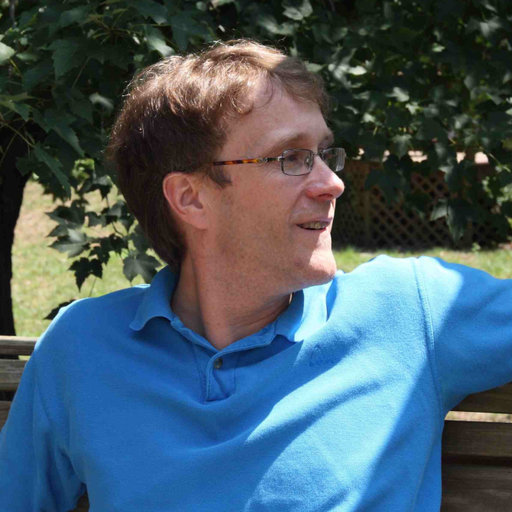
\includegraphics[height=.32\textheight]{mhc.jpg}}\\
\subfloat[Philip Wu (PhD, shallow water + GPU)]{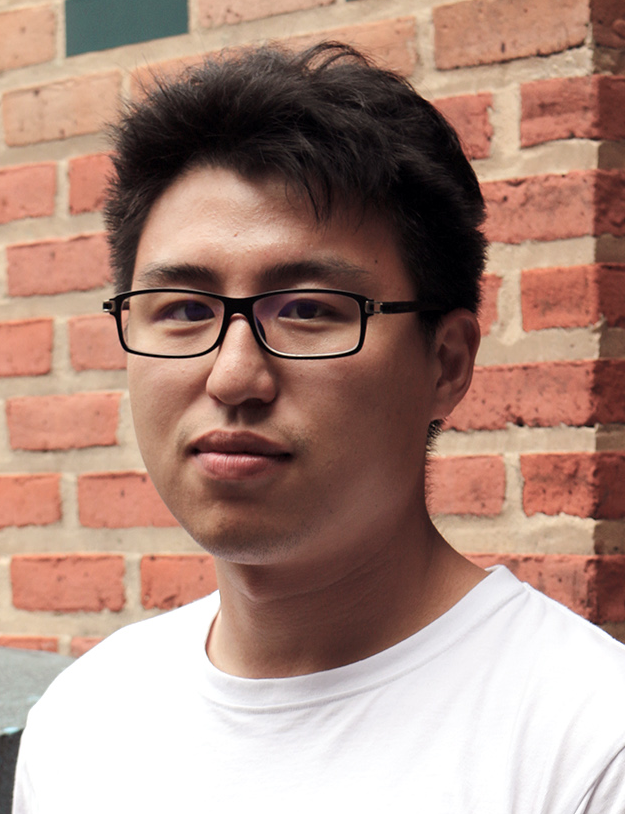
\includegraphics[height=.32\textheight]{pw.png}\hspace{.5em}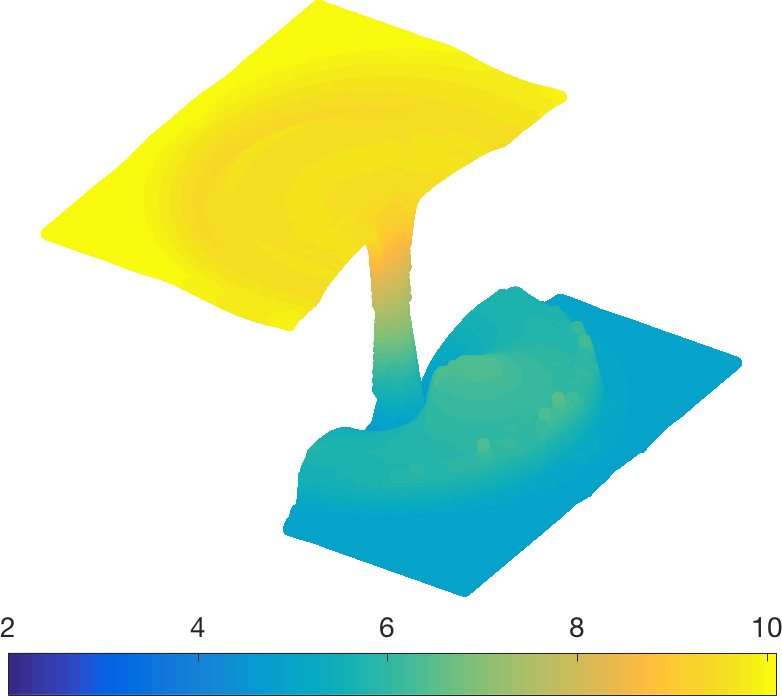
\includegraphics[height=.32\textheight]{Dam3.png}}
\end{figure}
}


\frame{
\frametitle{High order finite element methods for hyperbolic PDEs}
\setcounter{subfigure}{0}
\vspace{-1.5em}
\begin{overlayarea}{\textwidth}{.8\textheight}
\begin{columns}
\begin{column}{.5\textwidth}
\begin{itemize}
\item<1-> Aerodynamics applications: acoustics, vorticular flows, turbulence, shocks.
\vspace{1em}
\item<1-> Goal: \note{accurate} simulations on \note{unstructured meshes}.   
\vspace{1em}
\item<2-> Discontinuous Galerkin (DG) methods: geometric flexibility, high order accuracy.
%\item<2-> High order: low numerical dissipation and dispersion.
%\vspace{.5em}
%\item<2-> High order approximations are more accurate per unknown.
%\vspace{.5em}
%\item<3-> High performance computing\\on many-core architectures (efficient explicit time-stepping).
\end{itemize}
\end{column}
\begin{column}{.05\textwidth}
%spacing
\end{column}
\begin{column}{.475\textwidth}
%\vspace{-2.5em}
\begin{figure}
\centering
\begin{overlayarea}{\textwidth}{.65\textheight}
\only<1>{
%\vspace{-1.5em}
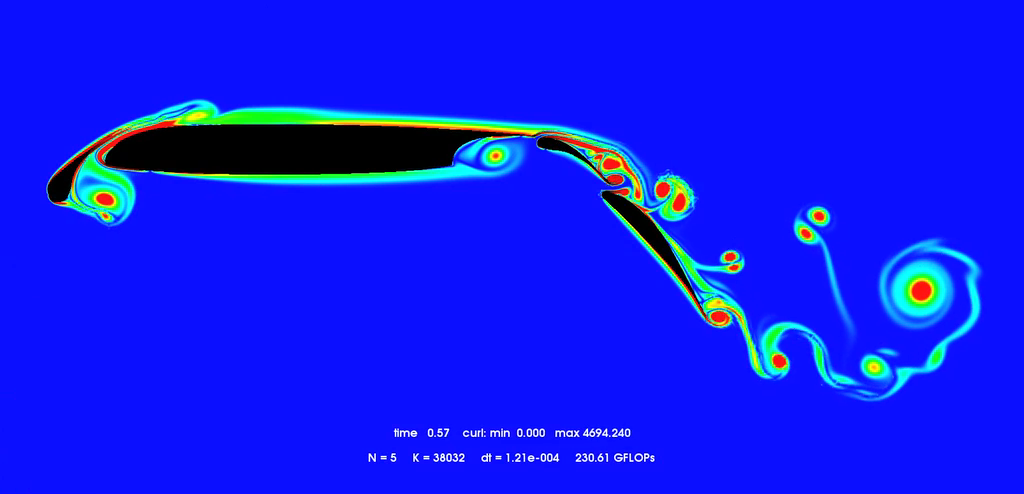
\includegraphics[width=.9\textwidth]{figs/wingflow.png}\\
\vspace{.25em}
\hspace{-.5em}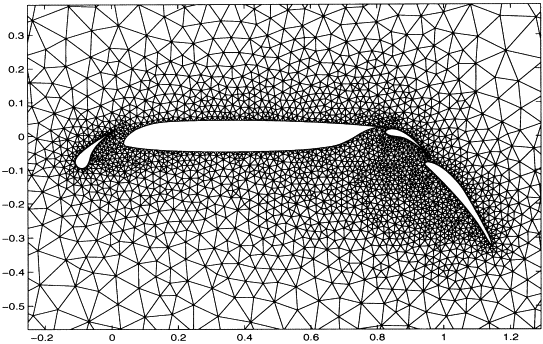
\includegraphics[width=.925\textwidth]{figs/fourfoil.png}
\caption*{\tiny Mesh from Slawig 2001.}
%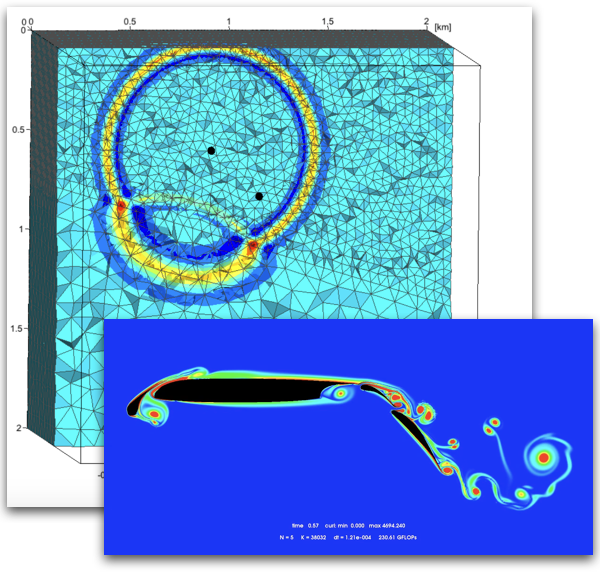
\includegraphics[width=\textwidth]{figs/vortexWave.png}
%%\hspace{-.25em}\hbox{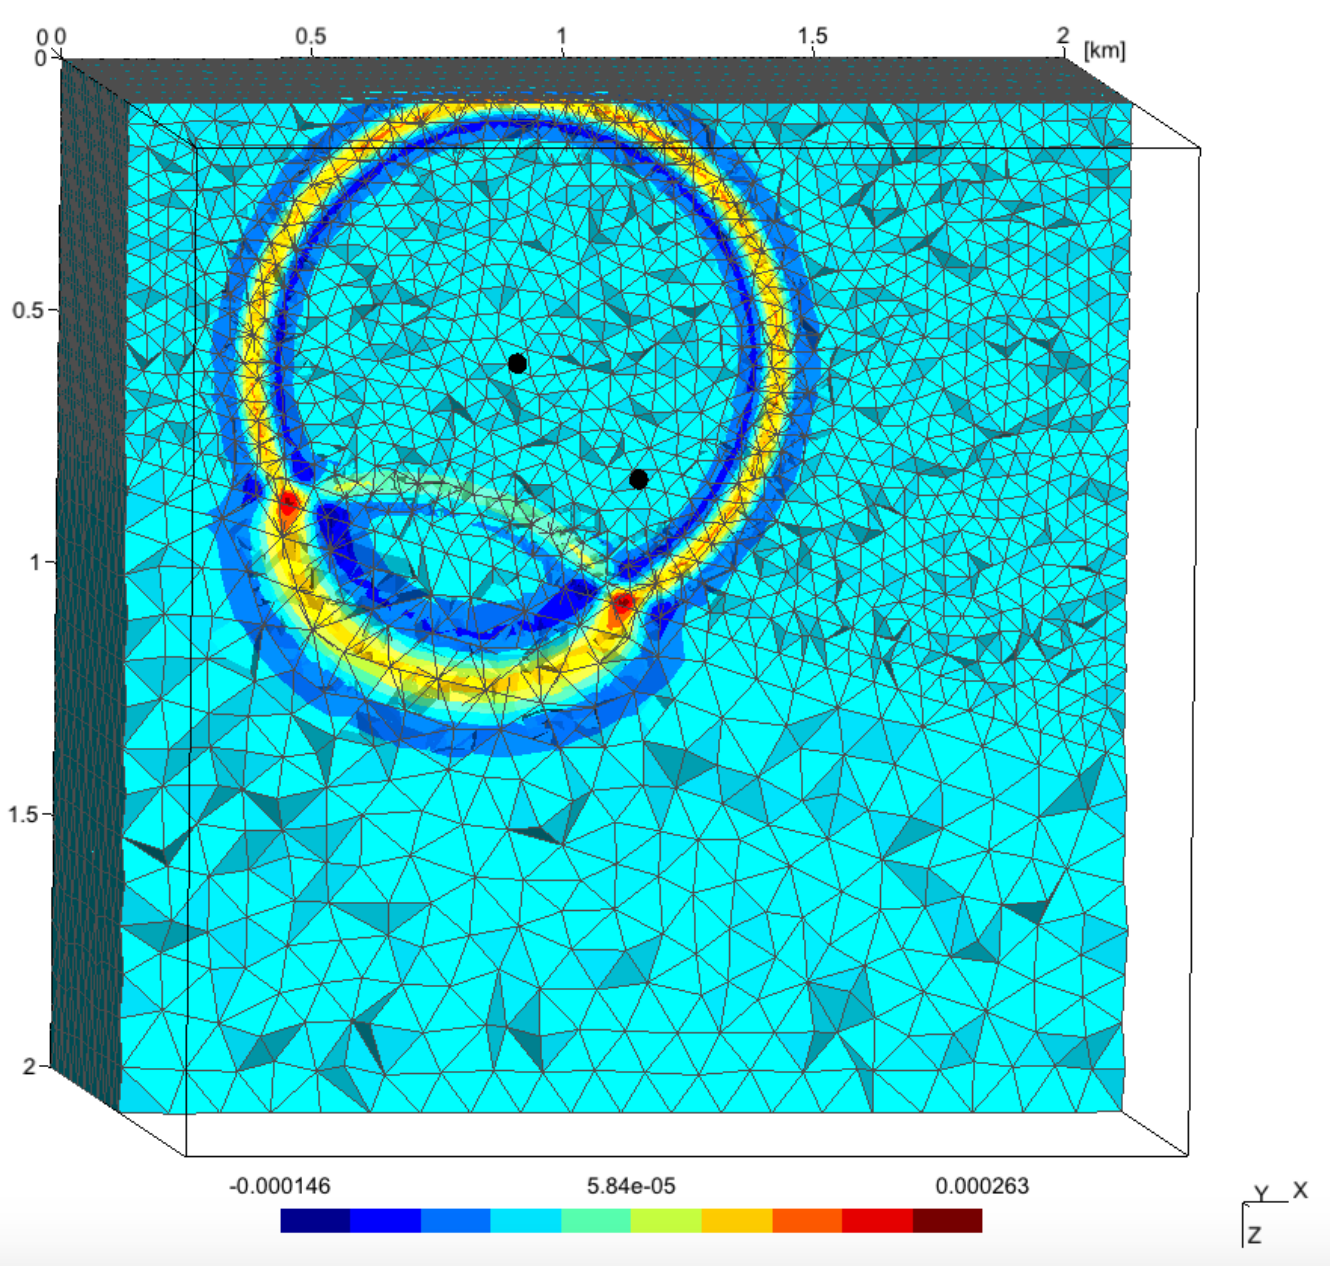
\includegraphics[width=.825\textwidth]{figs/wave.png}}\\
%%\vspace{-5.5em}
%%\hspace{10em}\hbox{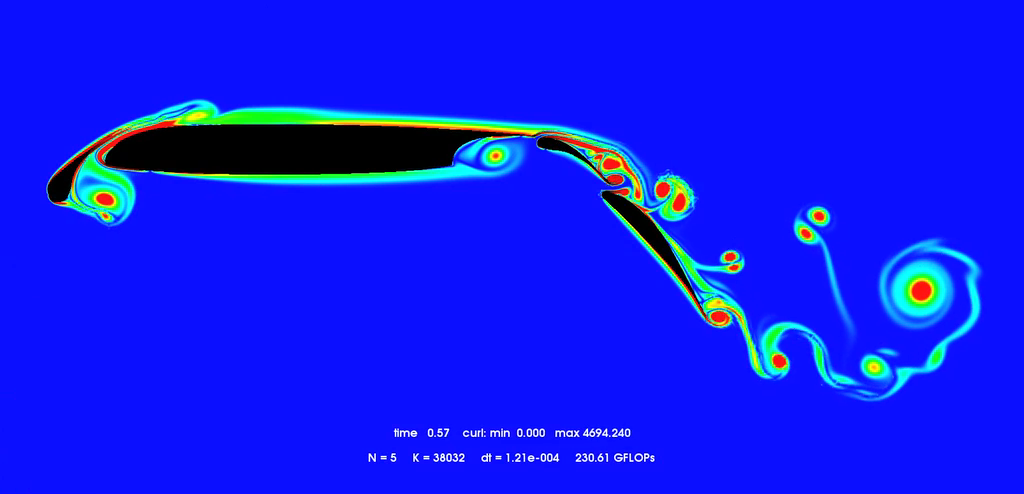
\includegraphics[width=.825\textwidth]{figs/wingflow.png}}
%\caption*{\tiny Figures courtesy of T.\ Warburton, A.\ Modave.}
}
\only<2>{
\vspace{2.5em}
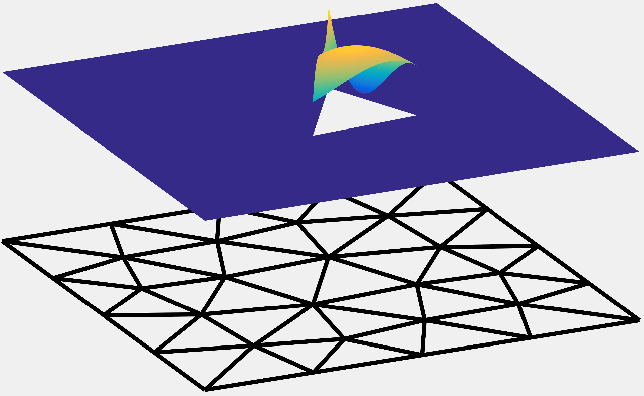
\includegraphics[width=.95\textwidth]{figs/dg.pdf}
}
%\only<2>{
%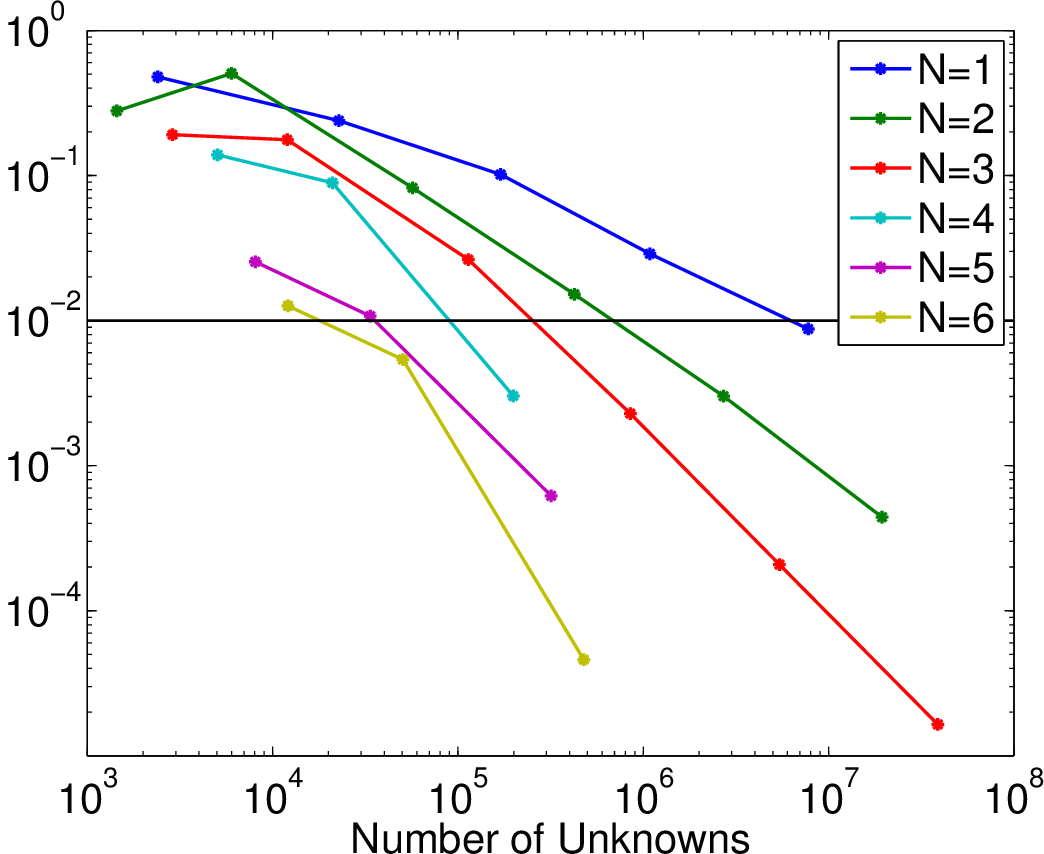
\includegraphics[width=.95\textwidth]{figs/error_v_dofs.png}
%\caption*{\scriptsize For smooth solutions, high order methods deliver a lower error per degree of freedom.}
%%\includegraphics[width=.95\textwidth]{figs/wave_N1.eps}
%%\caption*{\textbf{Fine} linear approximation.}
%}
%\only<3->{
%\vspace{1em}
%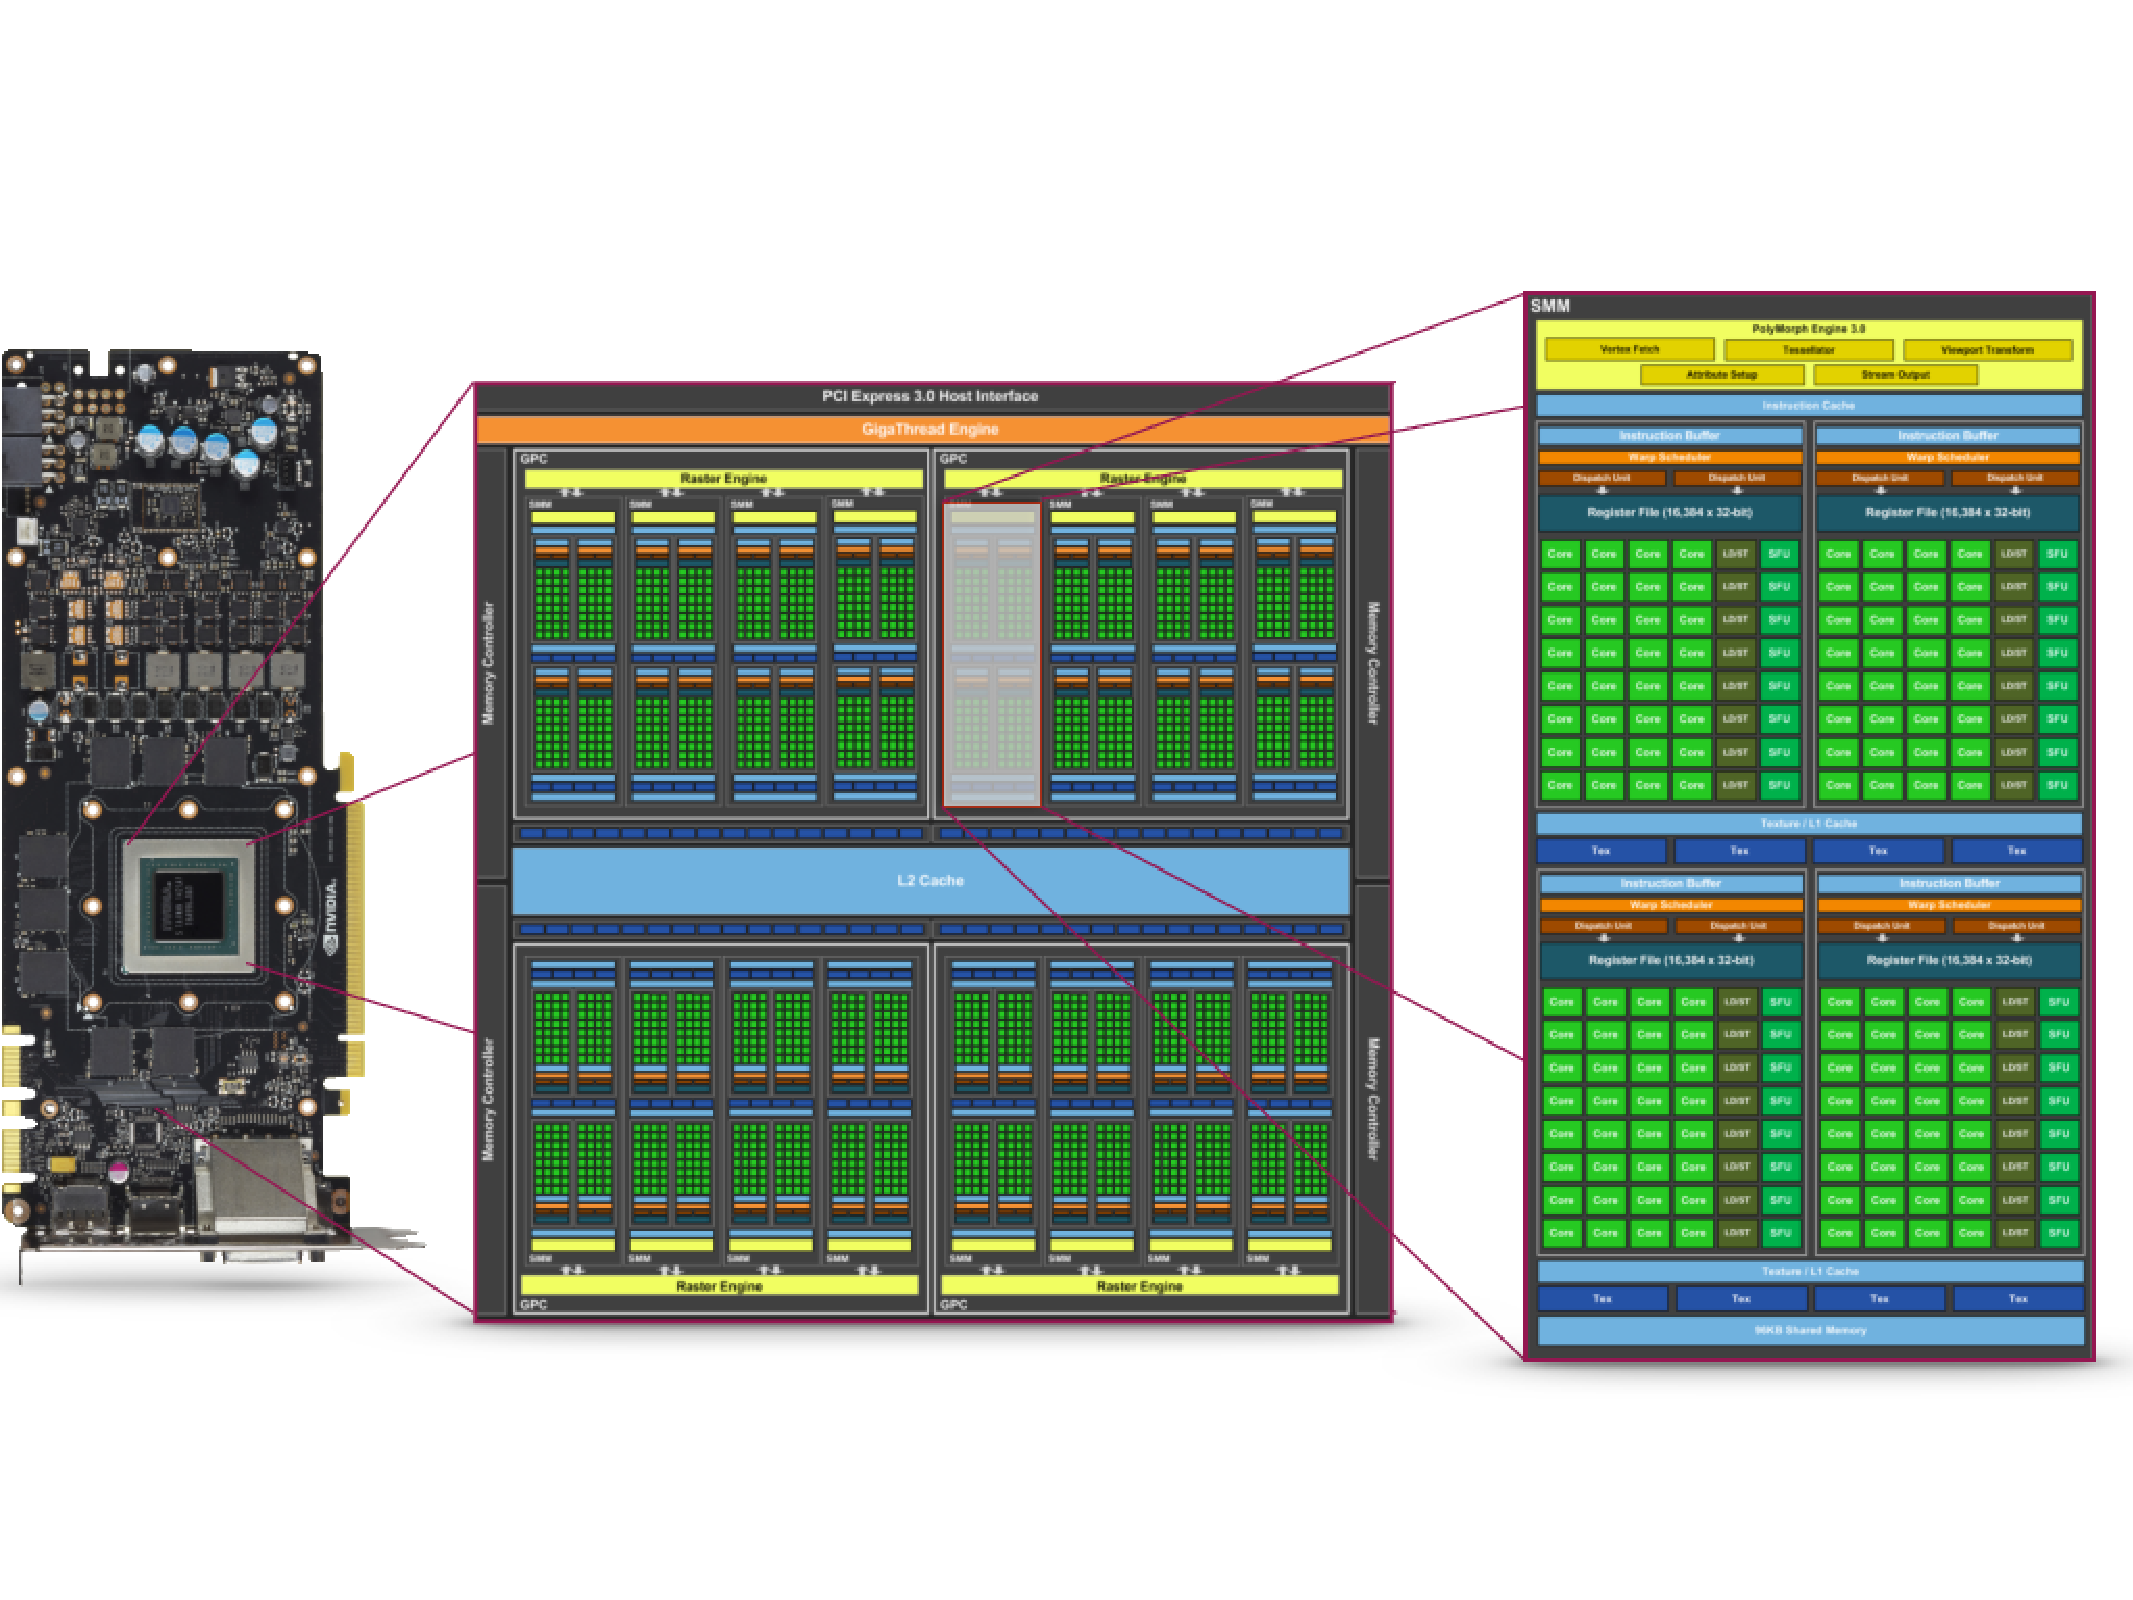
\includegraphics[width=.975\textwidth]{figs/gpu.pdf}
%\caption*{\footnotesize Schematic of an NVIDIA graphics processing unit (GPU).}
%}
%\caption*{Image courtesy of Axel Modave.}
\end{overlayarea}
\end{figure}
\end{column}
\end{columns}
%\vspace{1.5em}
%\uncover<7>{
%\begin{center}
%\ovalbox{Goal: address the \note{stability} of efficient high order methods.}
%\end{center}
%}
\end{overlayarea}
%\visible<1>{\let\thefootnote\relax\footnotetext[1]{\tiny Figures courtesy of T.\ Warburton, A.\ Modave.}}
%\visible<5>{\let\thefootnote\relax\footnotetext[5]{\tiny Figure courtesy of T.\ Warburton, Nvidia.}}
}


%\frame{
%\frametitle{Why high order discontinuous Galerkin methods?}
%
%\vspace{-.5em}
%\begin{columns}
%\begin{column}{.65\textwidth}
%Discontinuous Galerkin (DG) methods: 
%\vspace{.5em}
%\begin{itemize}
%\item Geometric flexibility, high order accuracy.
%\vspace{.5em}
%\item Weak continuity across faces.
%\end{itemize}
%\end{column}
%\begin{column}{.35\textwidth}
%\vspace{-.5em}
%\begin{figure}
%\centering
%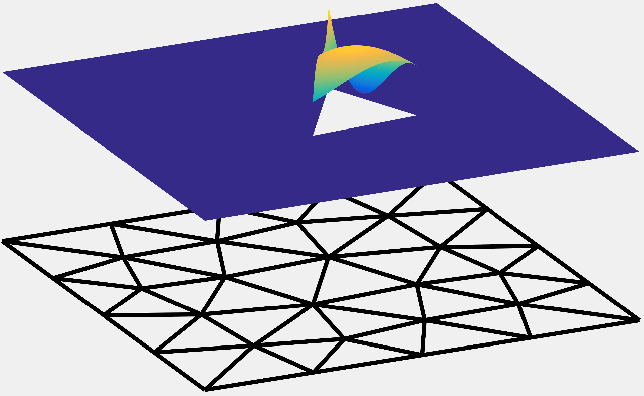
\includegraphics[width=\textwidth]{figs/dg.pdf}
%\end{figure}
%\end{column}
%\end{columns}
%
%\vspace{.5em}
%\begin{itemize}
%\item Example PDE: advection equation
%\[
%\pd{u}{t}{} = \pd{u}{x}{}.
%\]
%\item Local formulation with numerical flux $u^*$: find $u \in P^N\LRp{D^k}$ such that
%\[
%\int_{D_k}\pd{u}{t} \phi = \int_{D_k}\pd{u}{x}\phi + \int_{\partial D_k}{{n}_x\LRp{u^*-u}\phi}, \qquad \forall \phi \in P^N\LRp{D^k}.
%\]
%\end{itemize}
%}

\frame[noframenumbering]{
\frametitle{Why high order accuracy?}

\begin{figure}
\only<1>{
\setcounter{subfigure}{0}
\centering
\vspace{-.1em}
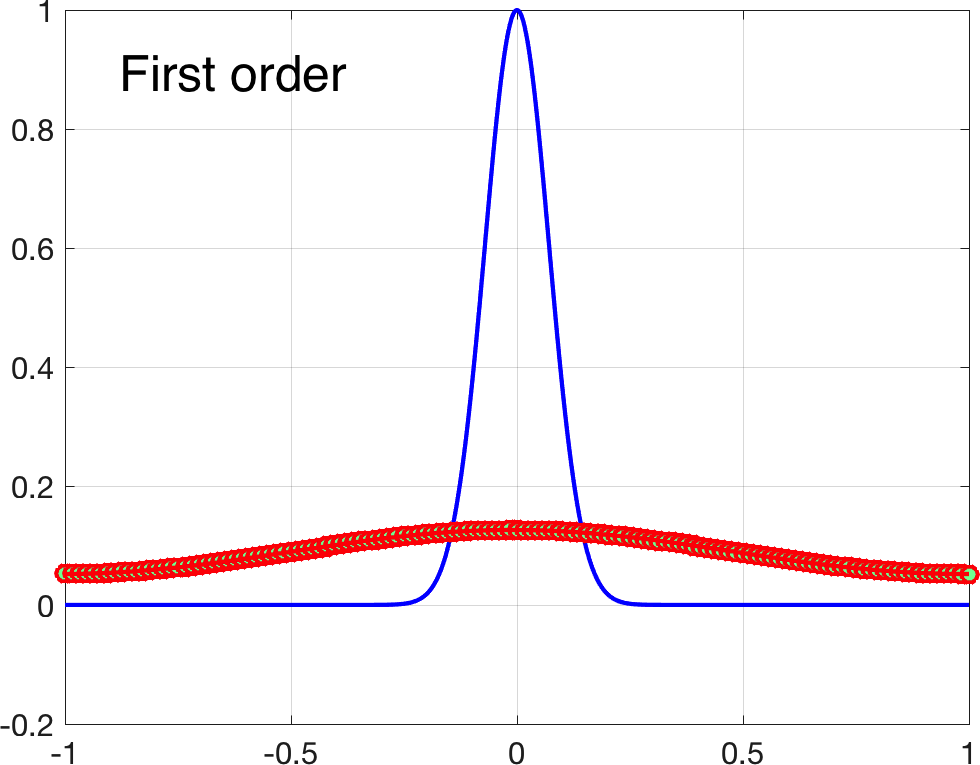
\includegraphics[width=.35\textwidth]{figs/advec1d_N0_diss.png}
\hspace{2em}
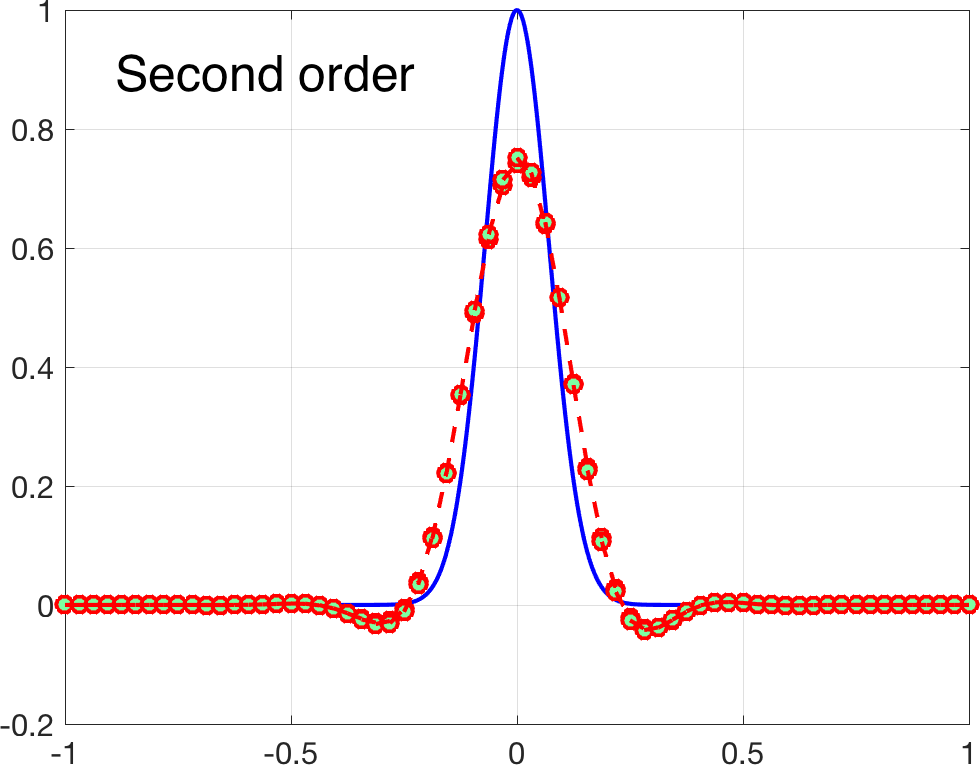
\includegraphics[width=.35\textwidth]{figs/advec1d_N1_diss.png}\\[.5em]
\hspace{.75em}
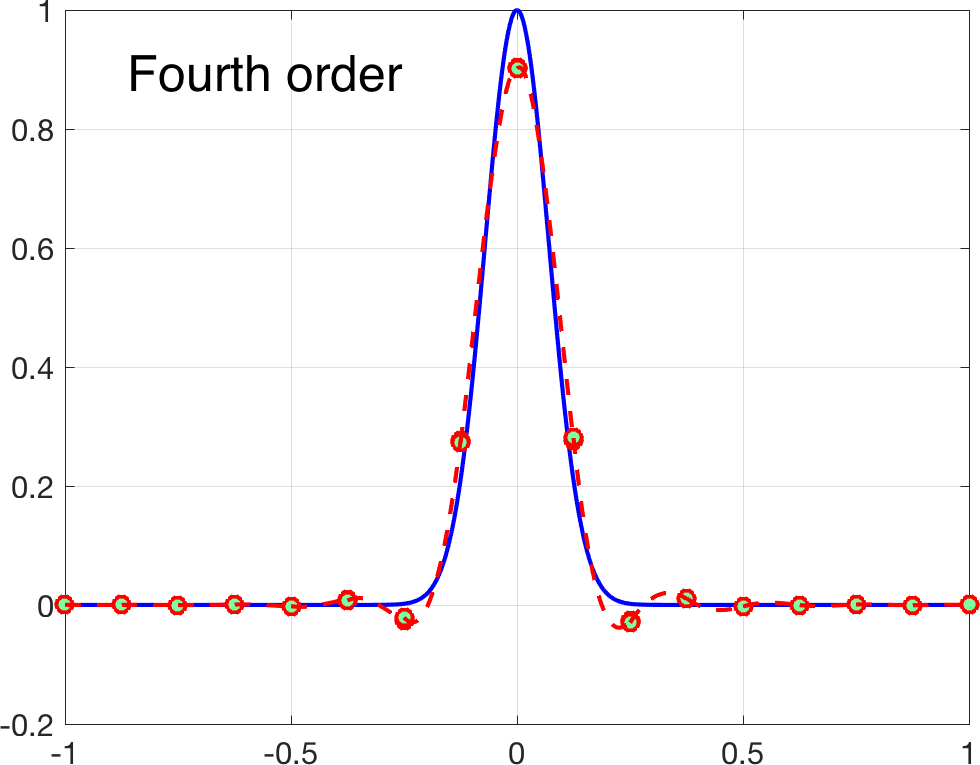
\includegraphics[width=.35\textwidth]{figs/advec1d_N3_diss.png}
\hspace{2em}
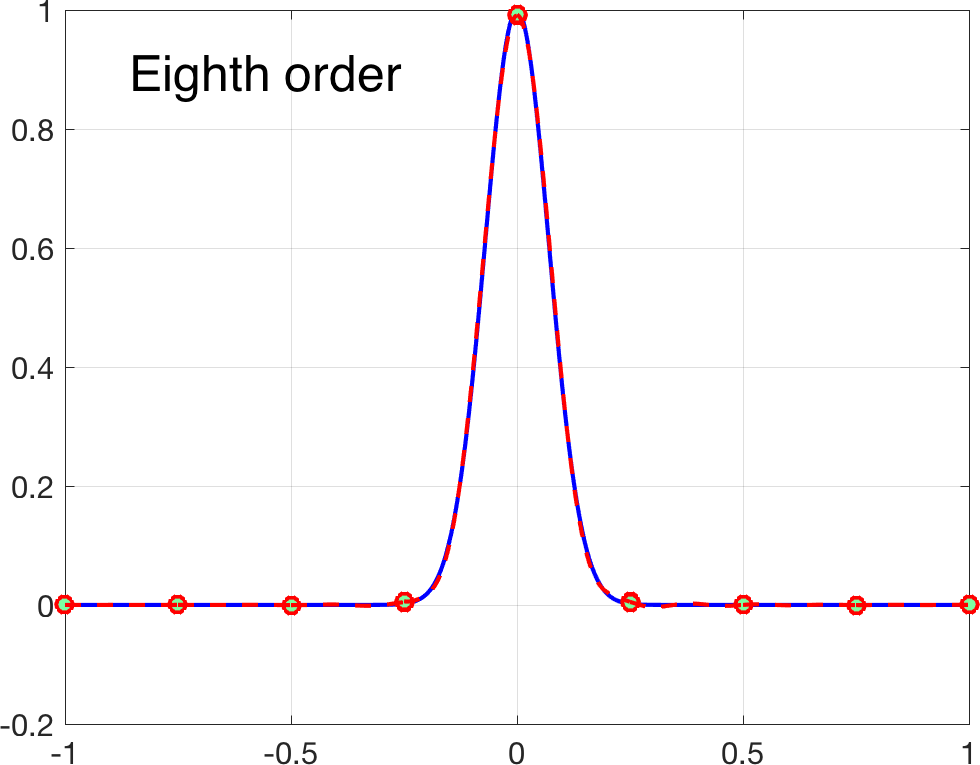
\includegraphics[width=.35\textwidth]{figs/advec1d_N7_diss.png}
}
%\only<2>{
%\centering
%\vspace{1em}
%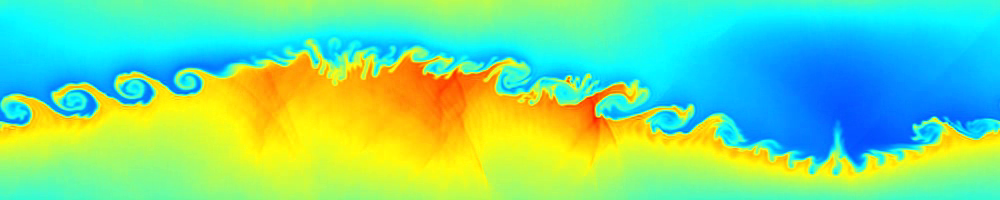
\includegraphics[width=.925\textwidth]{figs/turbulent1.png}\\
%\vspace{.5em}
%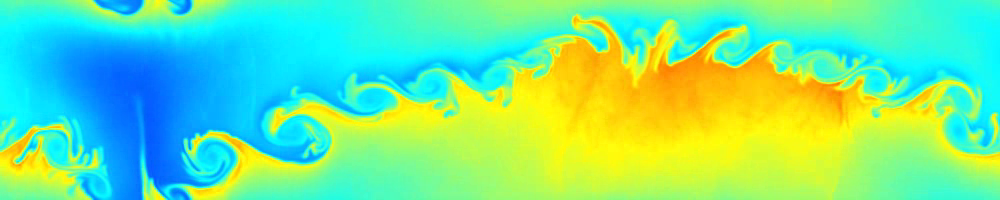
\includegraphics[width=.925\textwidth]{figs/turbulent2.png}
%\caption*{\footnotesize 8th order simulation of forced Kelvin-Helmholtz instability (Per-Olof Persson).  Vorticular structures and acoustic forcing are both sensitive to numerical dissipation.}
%}
\only<2>{
\centering
%\vspace{1em}
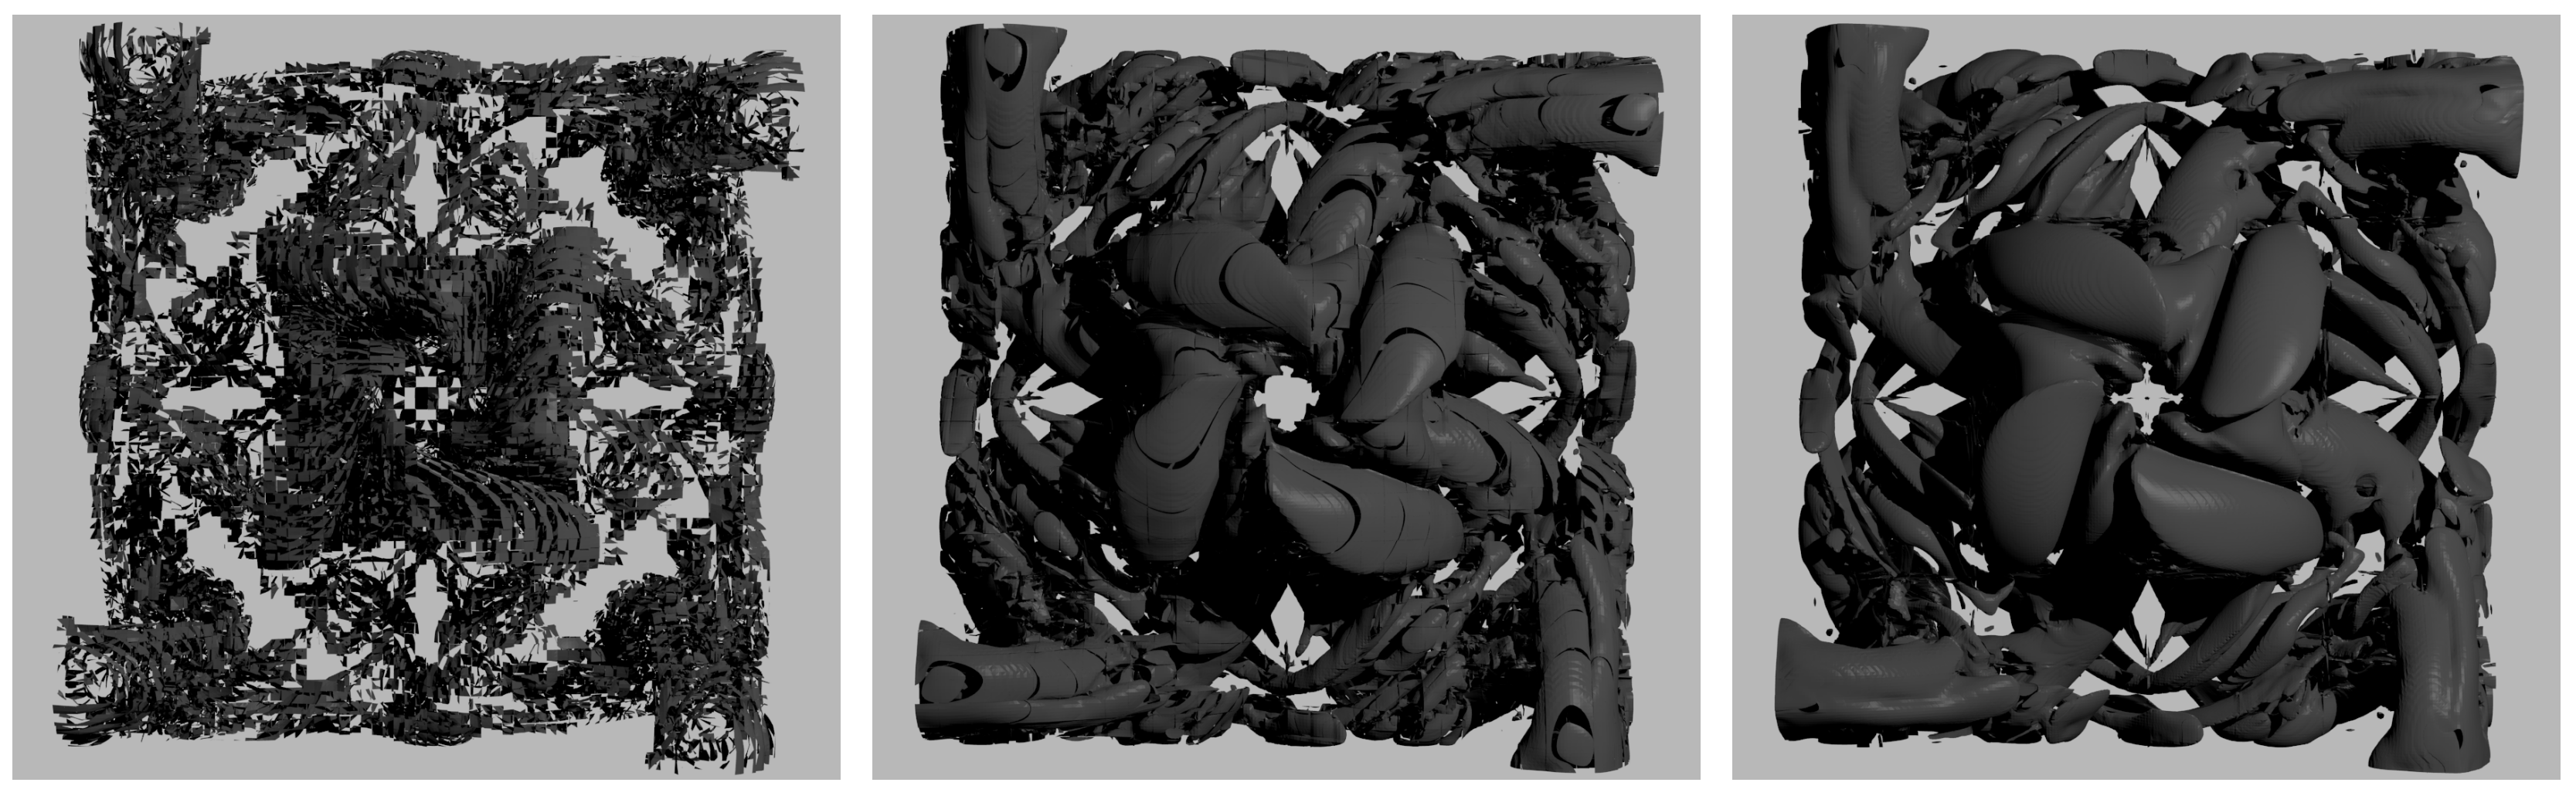
\includegraphics[width=.9\textwidth]{figs/beckgassner.png}\\
\vspace{.25em}
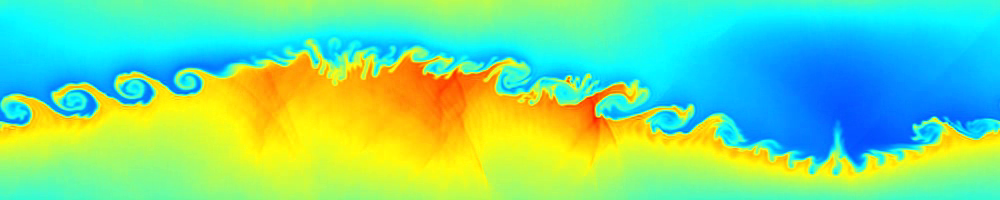
\includegraphics[width=.89\textwidth]{figs/turbulent1.png}%\\
%\vspace{.25em}
%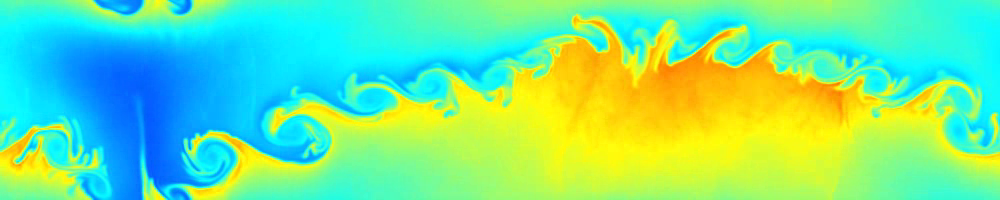
\includegraphics[width=.89\textwidth]{figs/turbulent2.png}
\caption*{\footnotesize 2nd, 4th, and 16th order Taylor-Green (top), 8th order Kelvin-Helmholtz (bottom).  Vorticular structures and acoustic waves are both sensitive to numerical dissipation.  Results from Beck and Gassner (2013) and Per-Olof Persson's website.}
}
\end{figure}

\only<1>{
\begin{center}
High order accurate resolution of propagating vortices and waves.
\end{center}
}

%\begin{center}
%Simplified explicit time-stepping (mass matrix inversion)
%\end{center}
%\only<4->{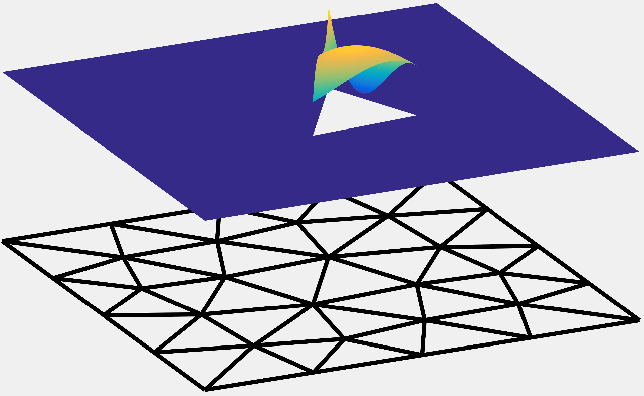
\includegraphics[width=.65\textwidth]{figs/dg.pdf}}
%\only<4>{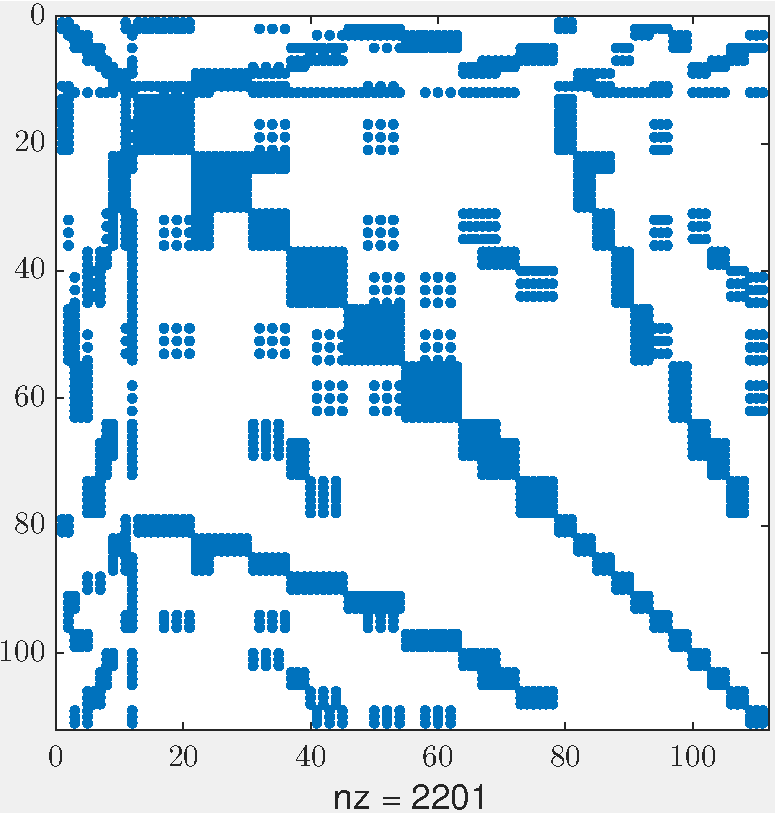
\includegraphics[width=.65\textwidth]{figs/MCG.pdf}\caption*{\footnotesize High order FEM mass matrix.}}
%\only<5>{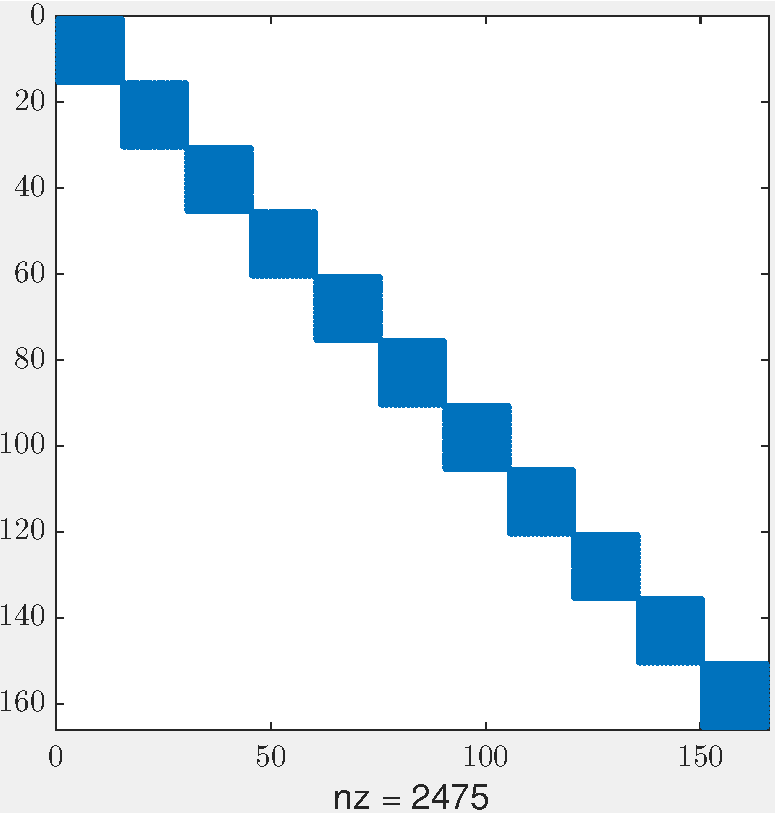
\includegraphics[width=.65\textwidth]{figs/MDG.pdf}\caption*{\footnotesize High order DG mass matrix.}}
}

\frame[noframenumbering]{
\frametitle{Why discontinuous Galerkin methods?}
%\vspace{-.1em}
\begin{figure}
\centering
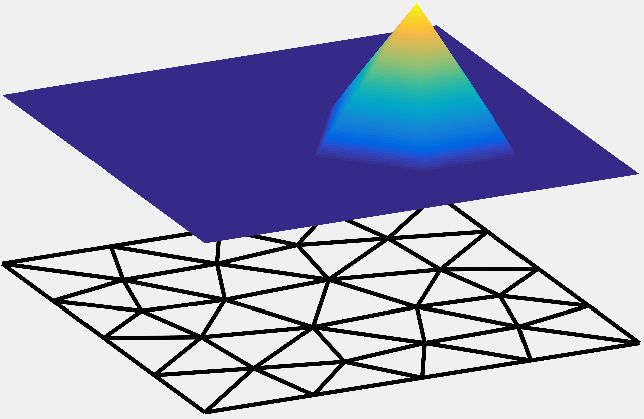
\includegraphics[width=.29\textwidth]{figs/cg.pdf}
\hspace{1em}
\raisebox{.15em}{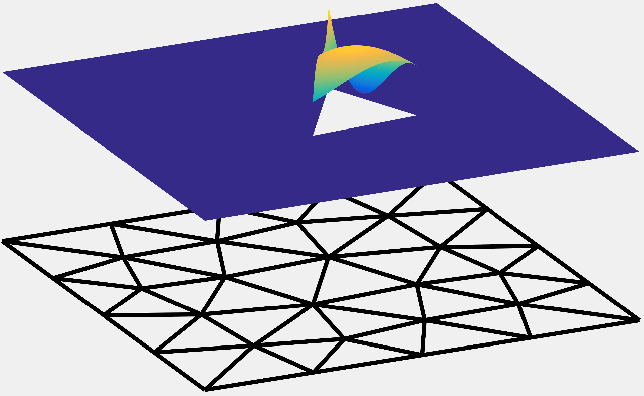
\includegraphics[width=.29\textwidth]{figs/dg.pdf}}\\
\subfloat[High order FEM]{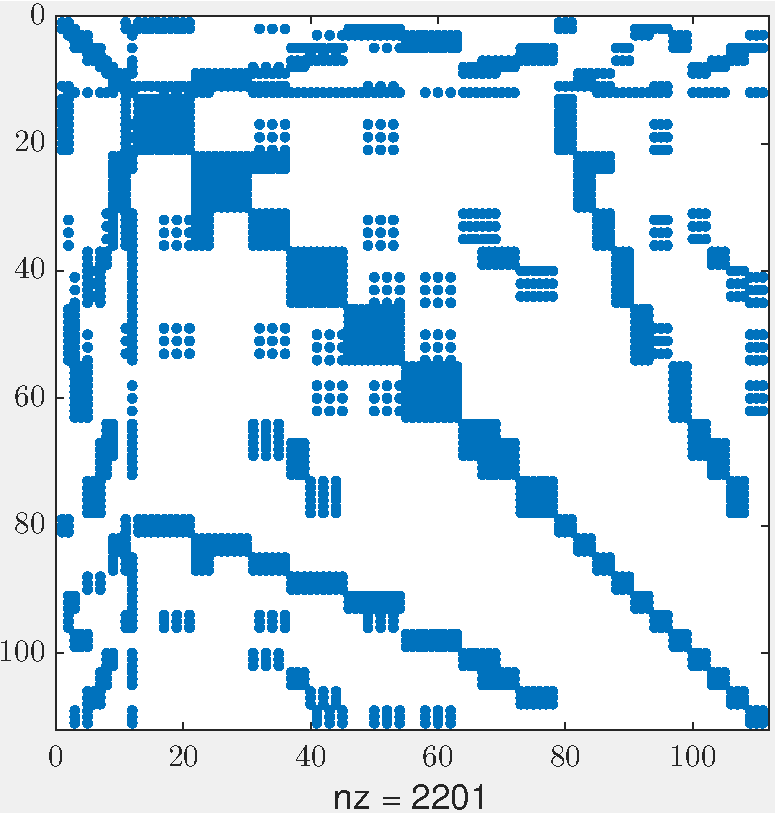
\includegraphics[width=.29\textwidth]{figs/MCG.pdf}}
\hspace{1em}
\subfloat[High order DG]{{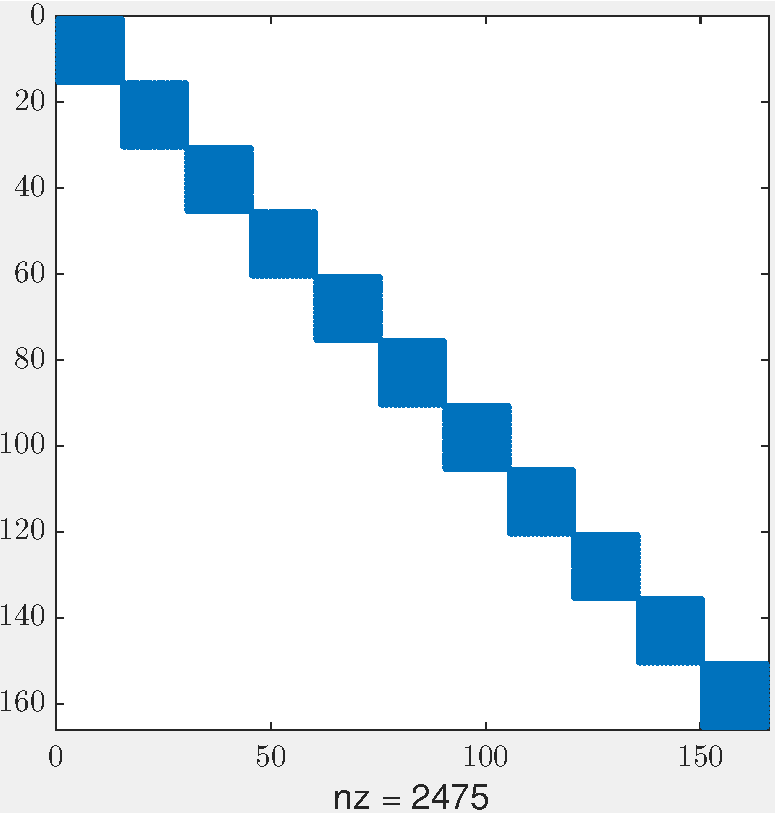
\includegraphics[width=.29\textwidth]{figs/MDG.pdf}}}
\caption*{\footnotesize The DG mass matrix is easily invertible for explicit time-stepping.}
\end{figure}

%\begin{center}
%Simplified explicit time-stepping (mass matrix inversion)
%\end{center}
%\only<4->{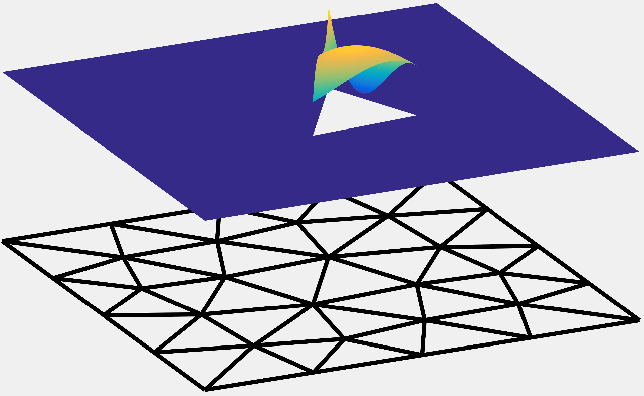
\includegraphics[width=.65\textwidth]{figs/dg.pdf}}
}



\frame{
\frametitle{Why \textit{not} high order DG methods?}
\setcounter{subfigure}{0}
\vspace{-1em}
\begin{figure}
\begin{overprint}
\centering
\foreach \id in {1,2,3,4}{%
\only<\id>{
\captionsetup[subfloat]{width=.45\textwidth, justification=centering}
\subfloat[Exact solution]{%[$N = 7, K = 8$ (aligned mesh)]{
\makebox[.425\textwidth]{\includegraphics[width=.4\textwidth]{figs/burgersStable_\id.png}}}%
\hspace{1em}%
\subfloat[8th order DG]{ %[$N = 7, K = 9$ (non-aligned mesh)]{
\makebox[.425\textwidth]{\includegraphics[width=.4\textwidth]{figs/burgersUnstable_\id.png}}}
} % only
} % foreach 
\end{overprint}
\end{figure}
%\vspace{-.5em}
\begin{itemize}
\item High order methods blow up for under-resolved solutions of \note{nonlinear conservation laws} (e.g., shocks and turbulence).   
\vspace{.25em}
\item Instability tied to loss of the \note{chain rule} + \note{quadrature error}.  
\end{itemize}
}

\frame{
\frametitle{Entropy stability for nonlinear problems}
\vspace{-.5em}
\begin{itemize}
\item Generalizes energy stability to \note{nonlinear} conservation laws (Burgers', shallow water, compressible Euler + Navier-Stokes, MHD).  
\[
\pd{\bm{u}}{t} + \pd{\bm{f}(\bm{u})}{x} = 0.  
\]
\item Continuous entropy inequality: given a convex \note{entropy} function $S(\bm{u})$ and ``entropy potential'' $\psi(\bm{u})$, test with $\bm{v}(\bm{u})$
\begin{align*}
&\int_{\Omega} \bm{v}^T\LRp{\pd{\bm{u}}{t} + \pd{\bm{f}(\bm{u})}{x}} = 0, \qquad \boxed{\bm{v}(\bm{u}) = \pd{S}{\bm{u}}} \\
&\Longrightarrow \int_{\Omega}\pd{S(\bm{u})}{t} + \LRu{\LRp{\bm{v}^T\bm{f}(\bm{u}) - \psi(\bm{u})}}_{-1}^1 \leq 0.
\end{align*}
\vspace{.01em}
\item Proof of entropy inequality relies on \note{chain rule}, integration by parts.  
\end{itemize}
}


\section{Entropy stable nodal summation-by-parts (SBP) schemes}

\frame[noframenumbering]{
\frametitle{Talk outline}
\tableofcontents
}
\frame[noframenumbering]{
\frametitle{Talk outline}
\tableofcontents[currentsection]
}

\frame{
\frametitle{Discretely entropy stable schemes}

Goal: improve robustness by enforcing a discrete entropy inequality.
\vspace{-.75em}
\begin{columns}
\begin{column}{.5\textwidth}

\begin{figure}
%\vspace{-1em}
\centering
%\only<1>{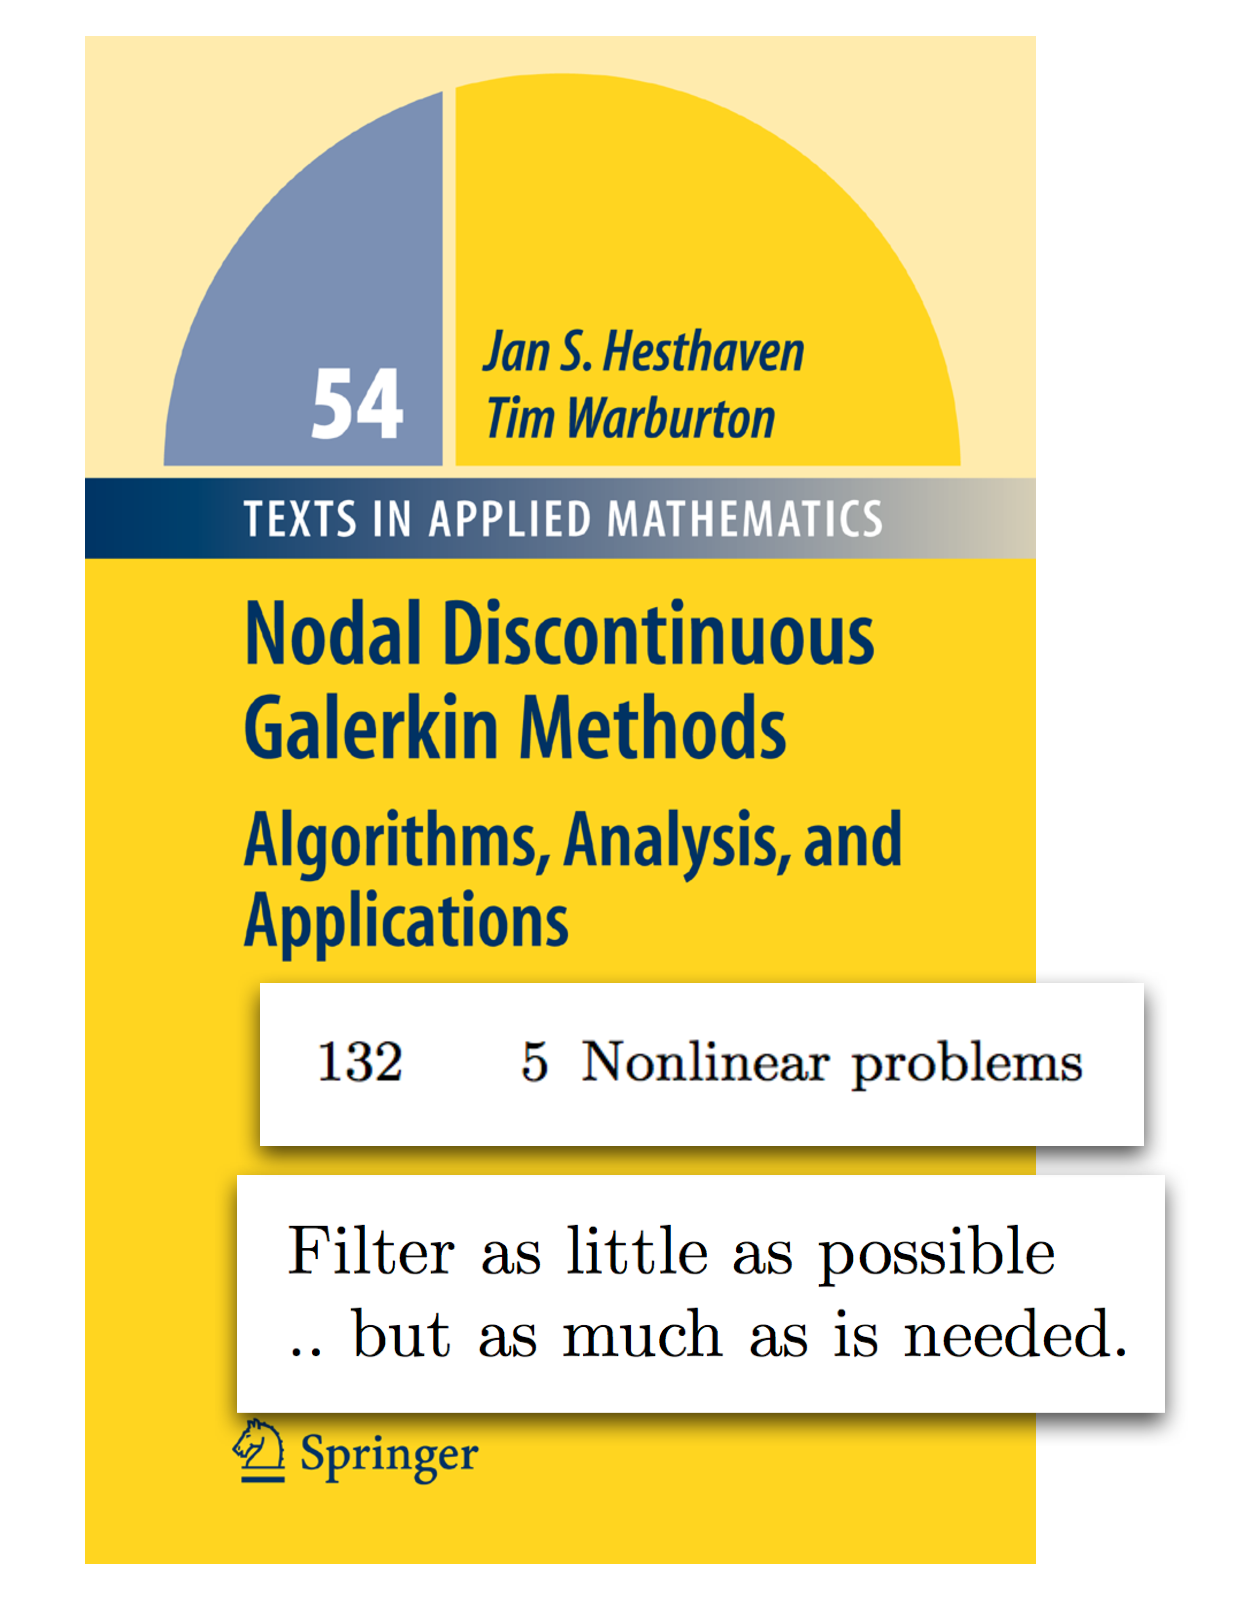
\includegraphics[width=.95\textwidth]{figs/ndgFilter.pdf}}
%\only<2>{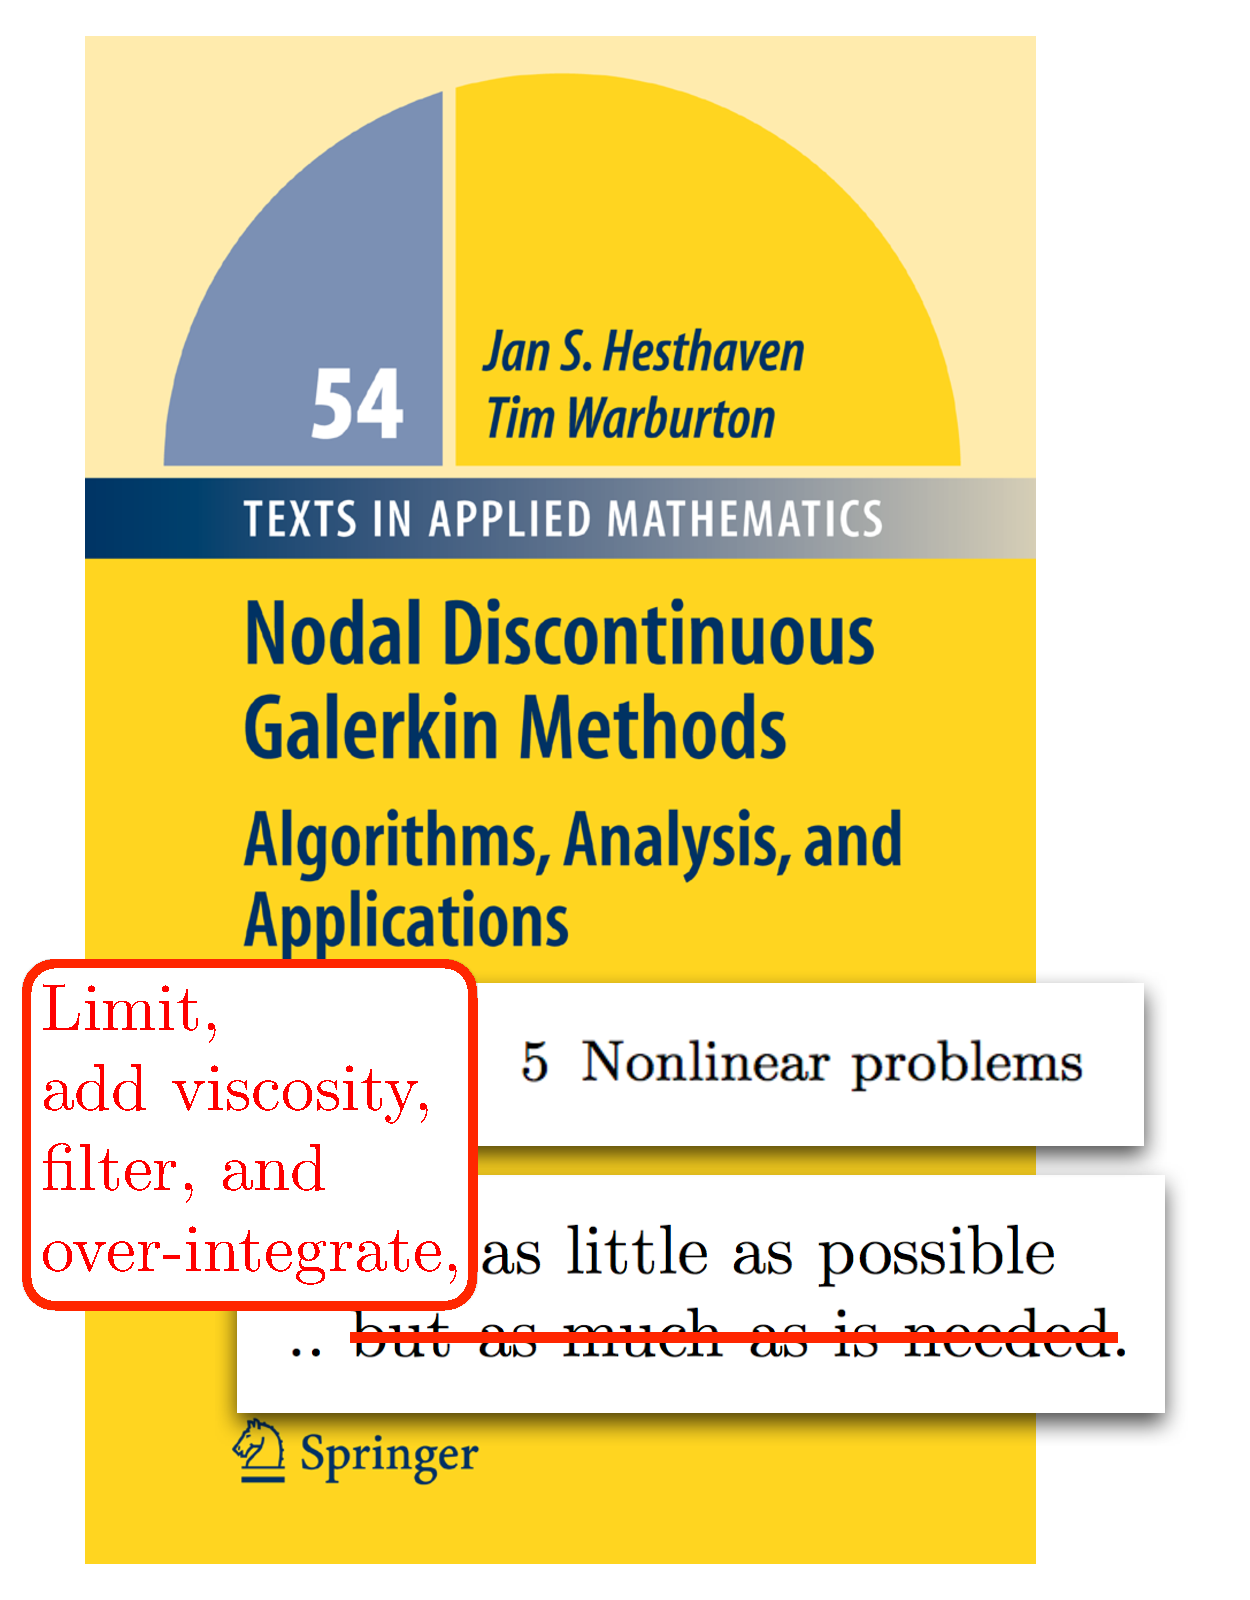
\includegraphics[width=.95\textwidth]{figs/ndgFilter2.pdf}}
%\hspace{1em}
\raisebox{.0em}{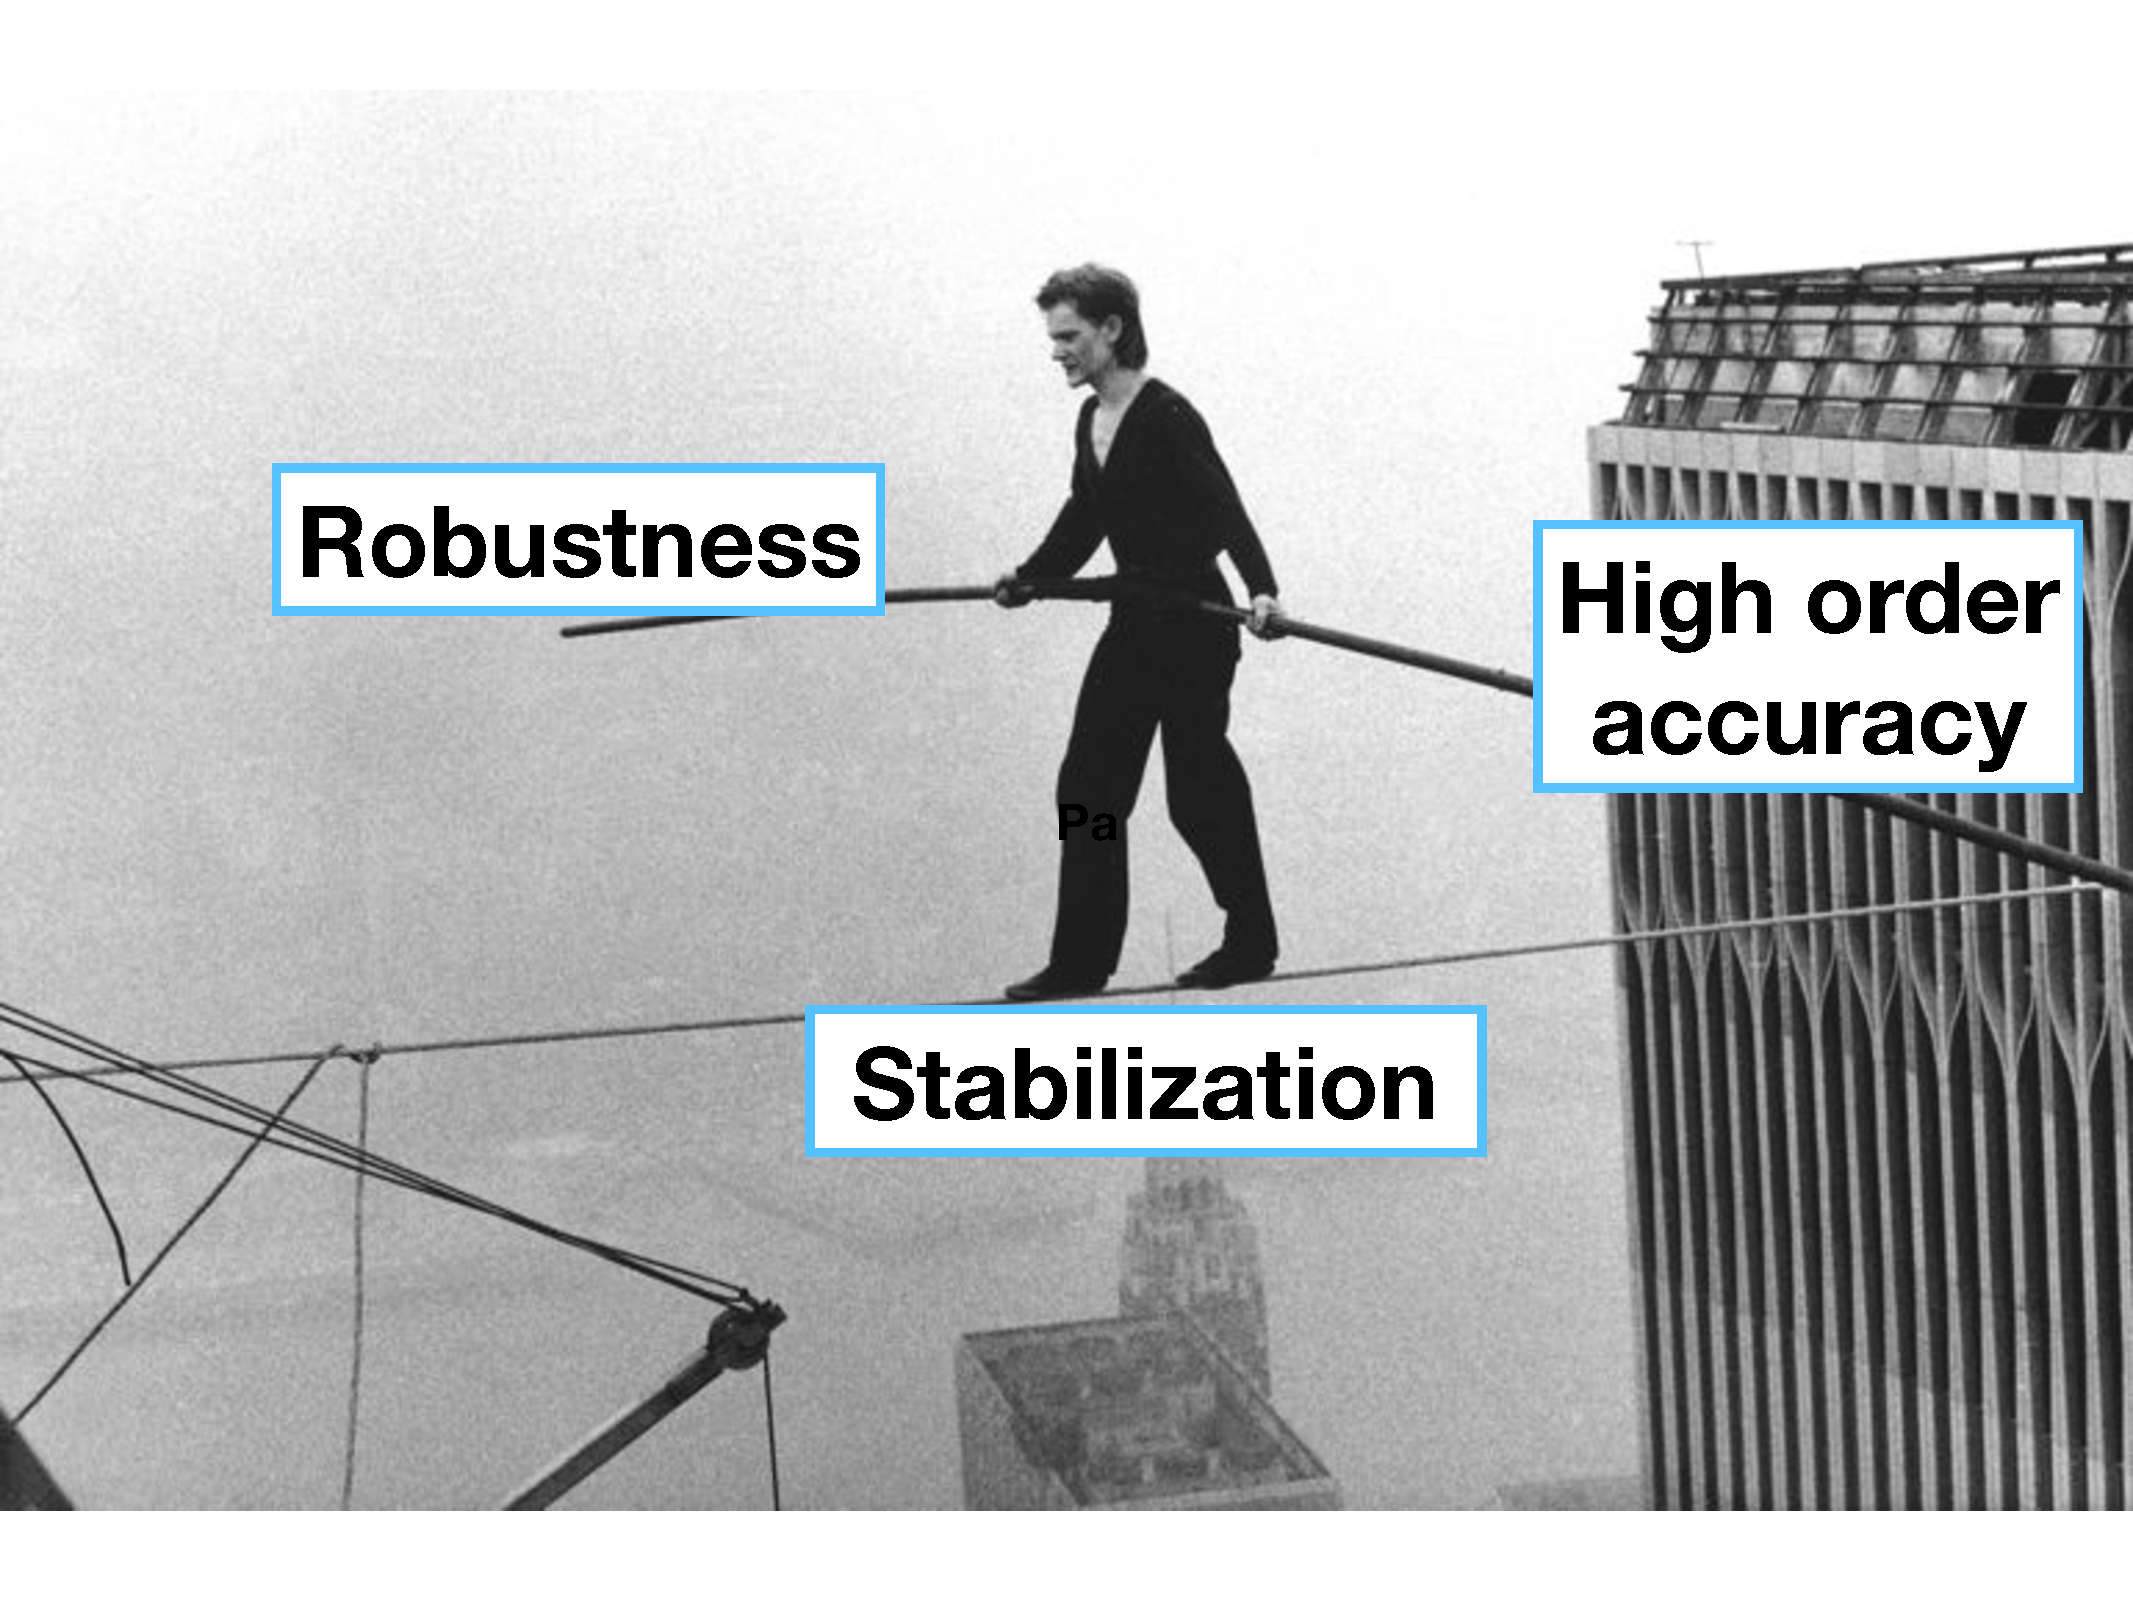
\includegraphics[width=\textwidth]{figs/balancing.pdf}}
\caption*{\tiny Image adapted from ``Man On Wire'' (2008)}
%\visible<5>{
\includegraphics[width=.475\textwidth]{figs/ductTape.png}}
\end{figure}

\end{column}
\begin{column}{.475\textwidth}
\begin{itemize}
\item<1-> Aim for stability {independently} of artificial viscosity, limiters.  %, discretization errors.
\vspace{.75em}
\item<1-> \textit{\note{Mechanical}} approach to stability based on algebraic discretization properties. 
%\vspace{.75em}
%\item<1-> Semi-discrete stability property for high order DG methods.  
\end{itemize}
\end{column}
\end{columns}

\let\thefootnote\relax\footnotetext{\tiny Finite volume methods: Tadmor, Chandrashekar, Ray, Svard, Fjordholm, Mishra, LeFloch, Rohde, \ldots}
\let\thefootnote\relax\footnotetext{\tiny High order tensor product elements: Fisher, Carpenter, Gassner, Winters, Kopriva, Hindenlang, Persson, Pazner, \ldots}
\let\thefootnote\relax\footnotetext{\tiny High order general elements: Chen and Shu, Crean, Hicken, DCDR Fernandez, Zingg, \ldots}
}

\frame{
\frametitle{Discretely entropy stable schemes: main ideas}

\begin{itemize}
\item<1-> Continuous and semi-discrete systems
\[
\boxed{\pd{\bm{u}}{t} + \pd{\bm{f}(\bm{u})}{x} - \epsilon \pdn{u}{x}{2}= 0} \quad \Longrightarrow \quad
\boxed{\bm{M}\td{\bm{u}}{t} + \bm{f}_x(\bm{u}) + \epsilon \bm{d}(\bm{u}) = \bm{0}}
%\boxed{\td{\bm{u}}{t} + \bm{D}\bm{f}(\bm{u}) + \epsilon \bm{K}\bm{u} = \bm{0}}
\]
\item<2-> Test with discrete entropy variables, use chain rule in time
\[
\underbrace{\bm{v}^T\bm{M}\td{\bm{u}}{t}}_{\bm{1}^T\bm{M}\td{S(\bm{u})}{t}} + \bm{v}^T\bm{f}_x(\bm{u}) + \epsilon \bm{v}^T\bm{d}(\bm{u}) = \bm{0}
%\boxed{\td{\bm{u}}{t} + \bm{D}\bm{f}(\bm{u}) + \epsilon \bm{K}\bm{u} = \bm{0}}
\]
\item<3-> Construct discretization s.t.\ (for periodic boundary conditions)
\[
\boxed{
\begin{array}{c}
\textcolor{red}{\bm{v}^T\bm{f}_x(\bm{u}) = 0}\\
\bm{v}^T\bm{d}(\bm{u}) \geq 0
\end{array}
} \qquad \Longrightarrow \qquad \bm{1}^T\bm{M}\td{S(\bm{u})}{t} = -\epsilon \bm{v}^T\bm{d}(\bm{u}) \leq 0.
\]
\end{itemize}
}

\frame{
\frametitle{Examples of high order entropy stable simulations}
\vspace{-.5em}
\begin{figure}
\centering
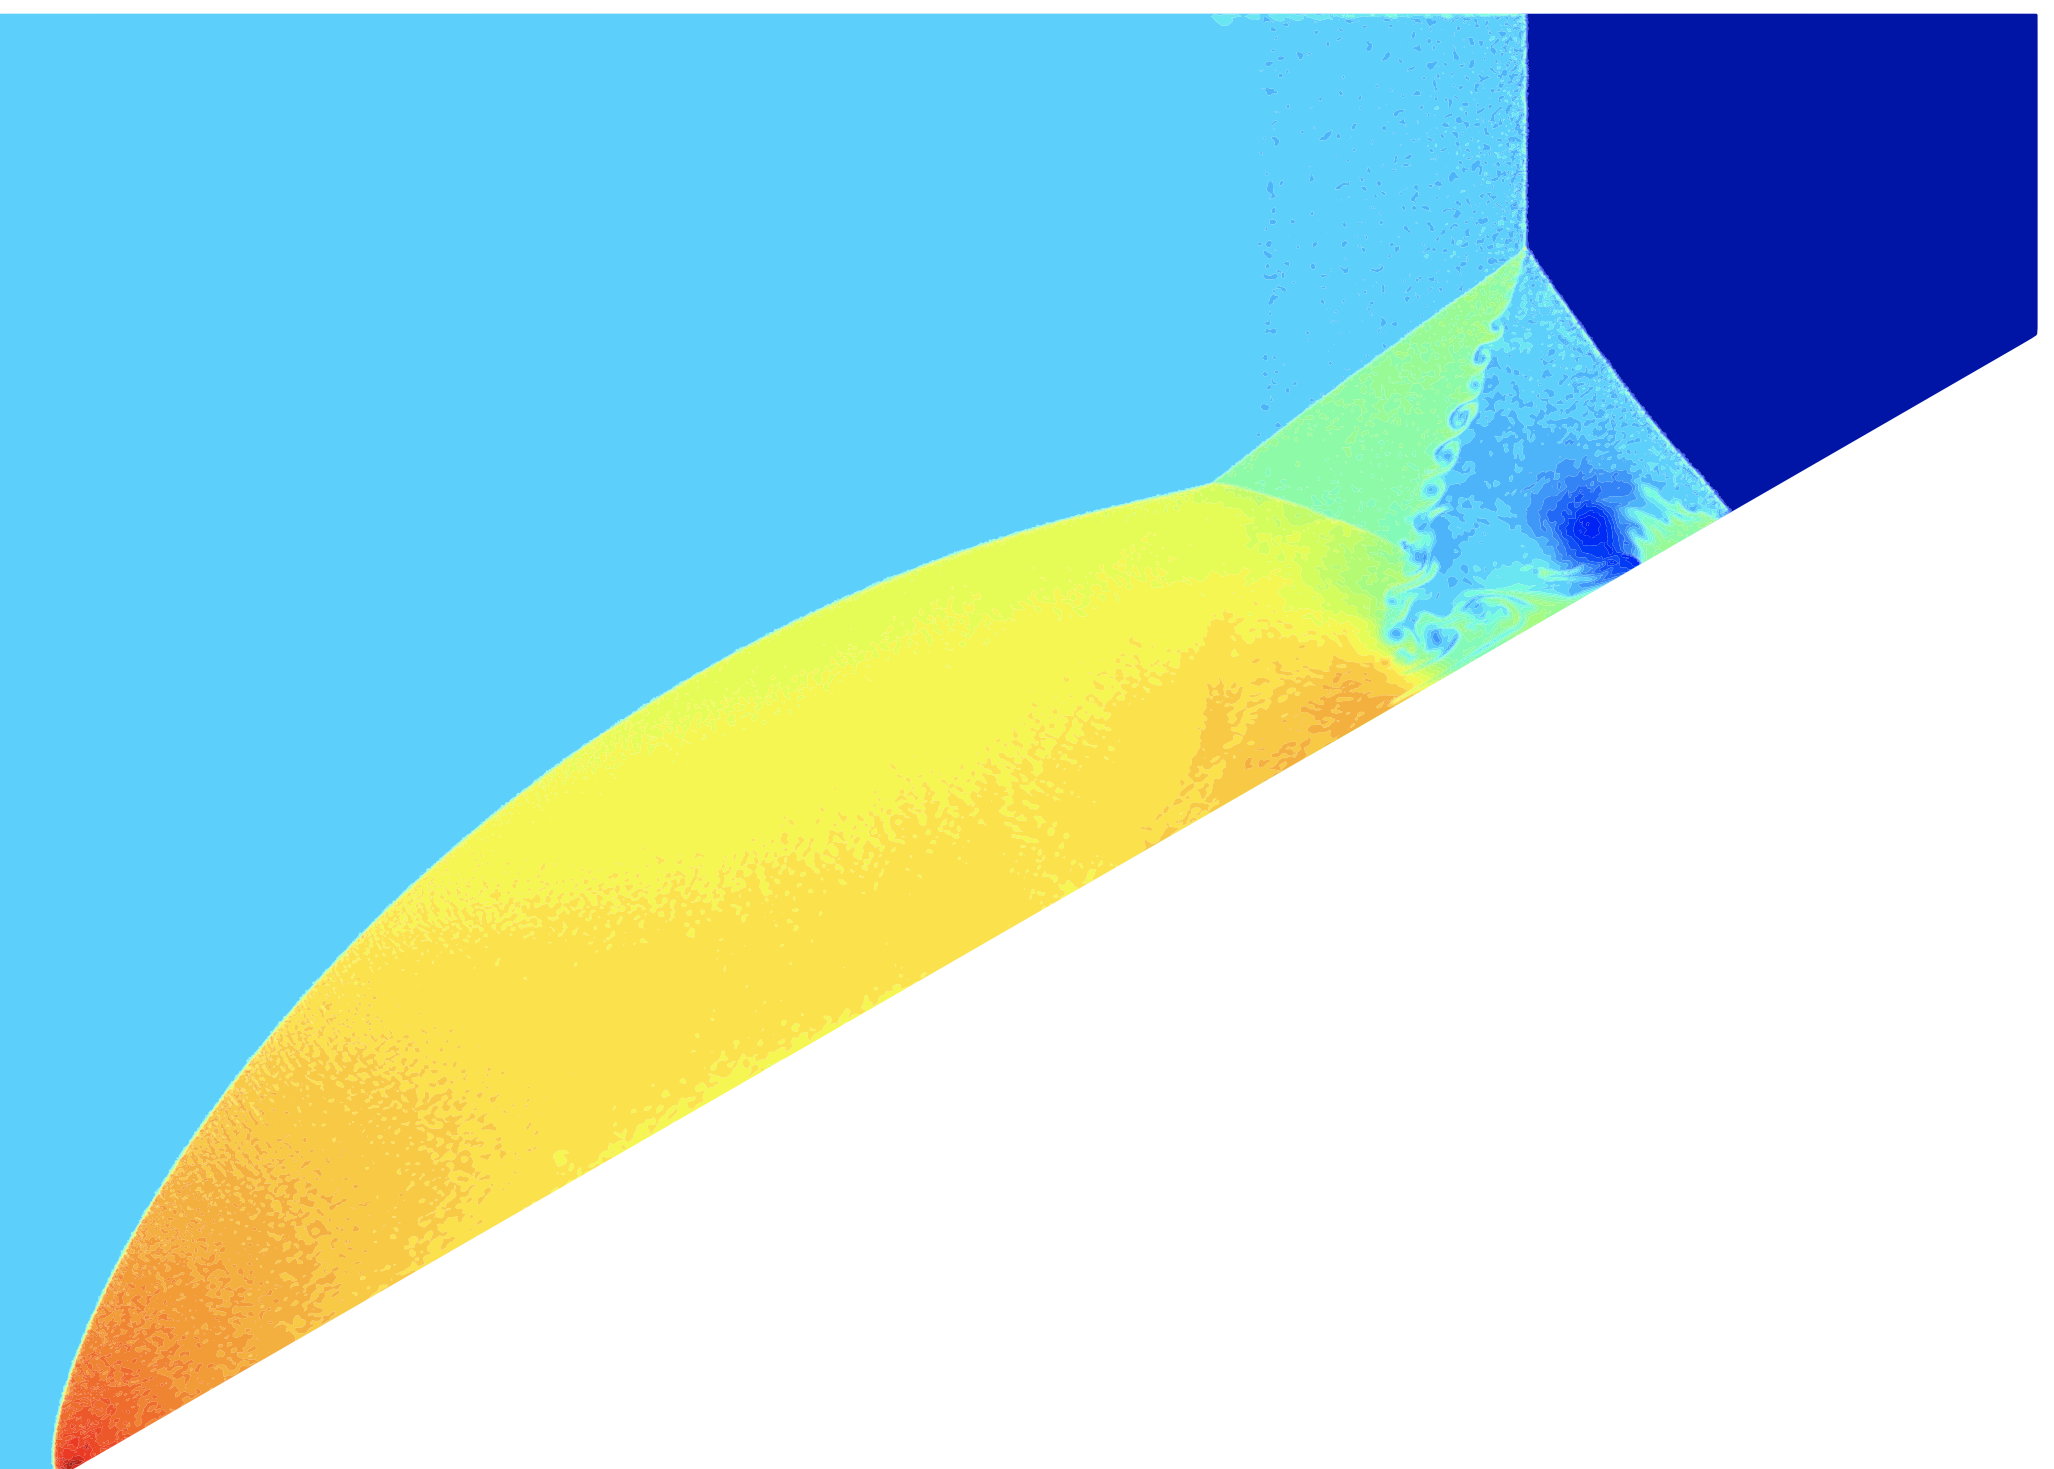
\includegraphics[width=.38\textwidth]{shu.png}
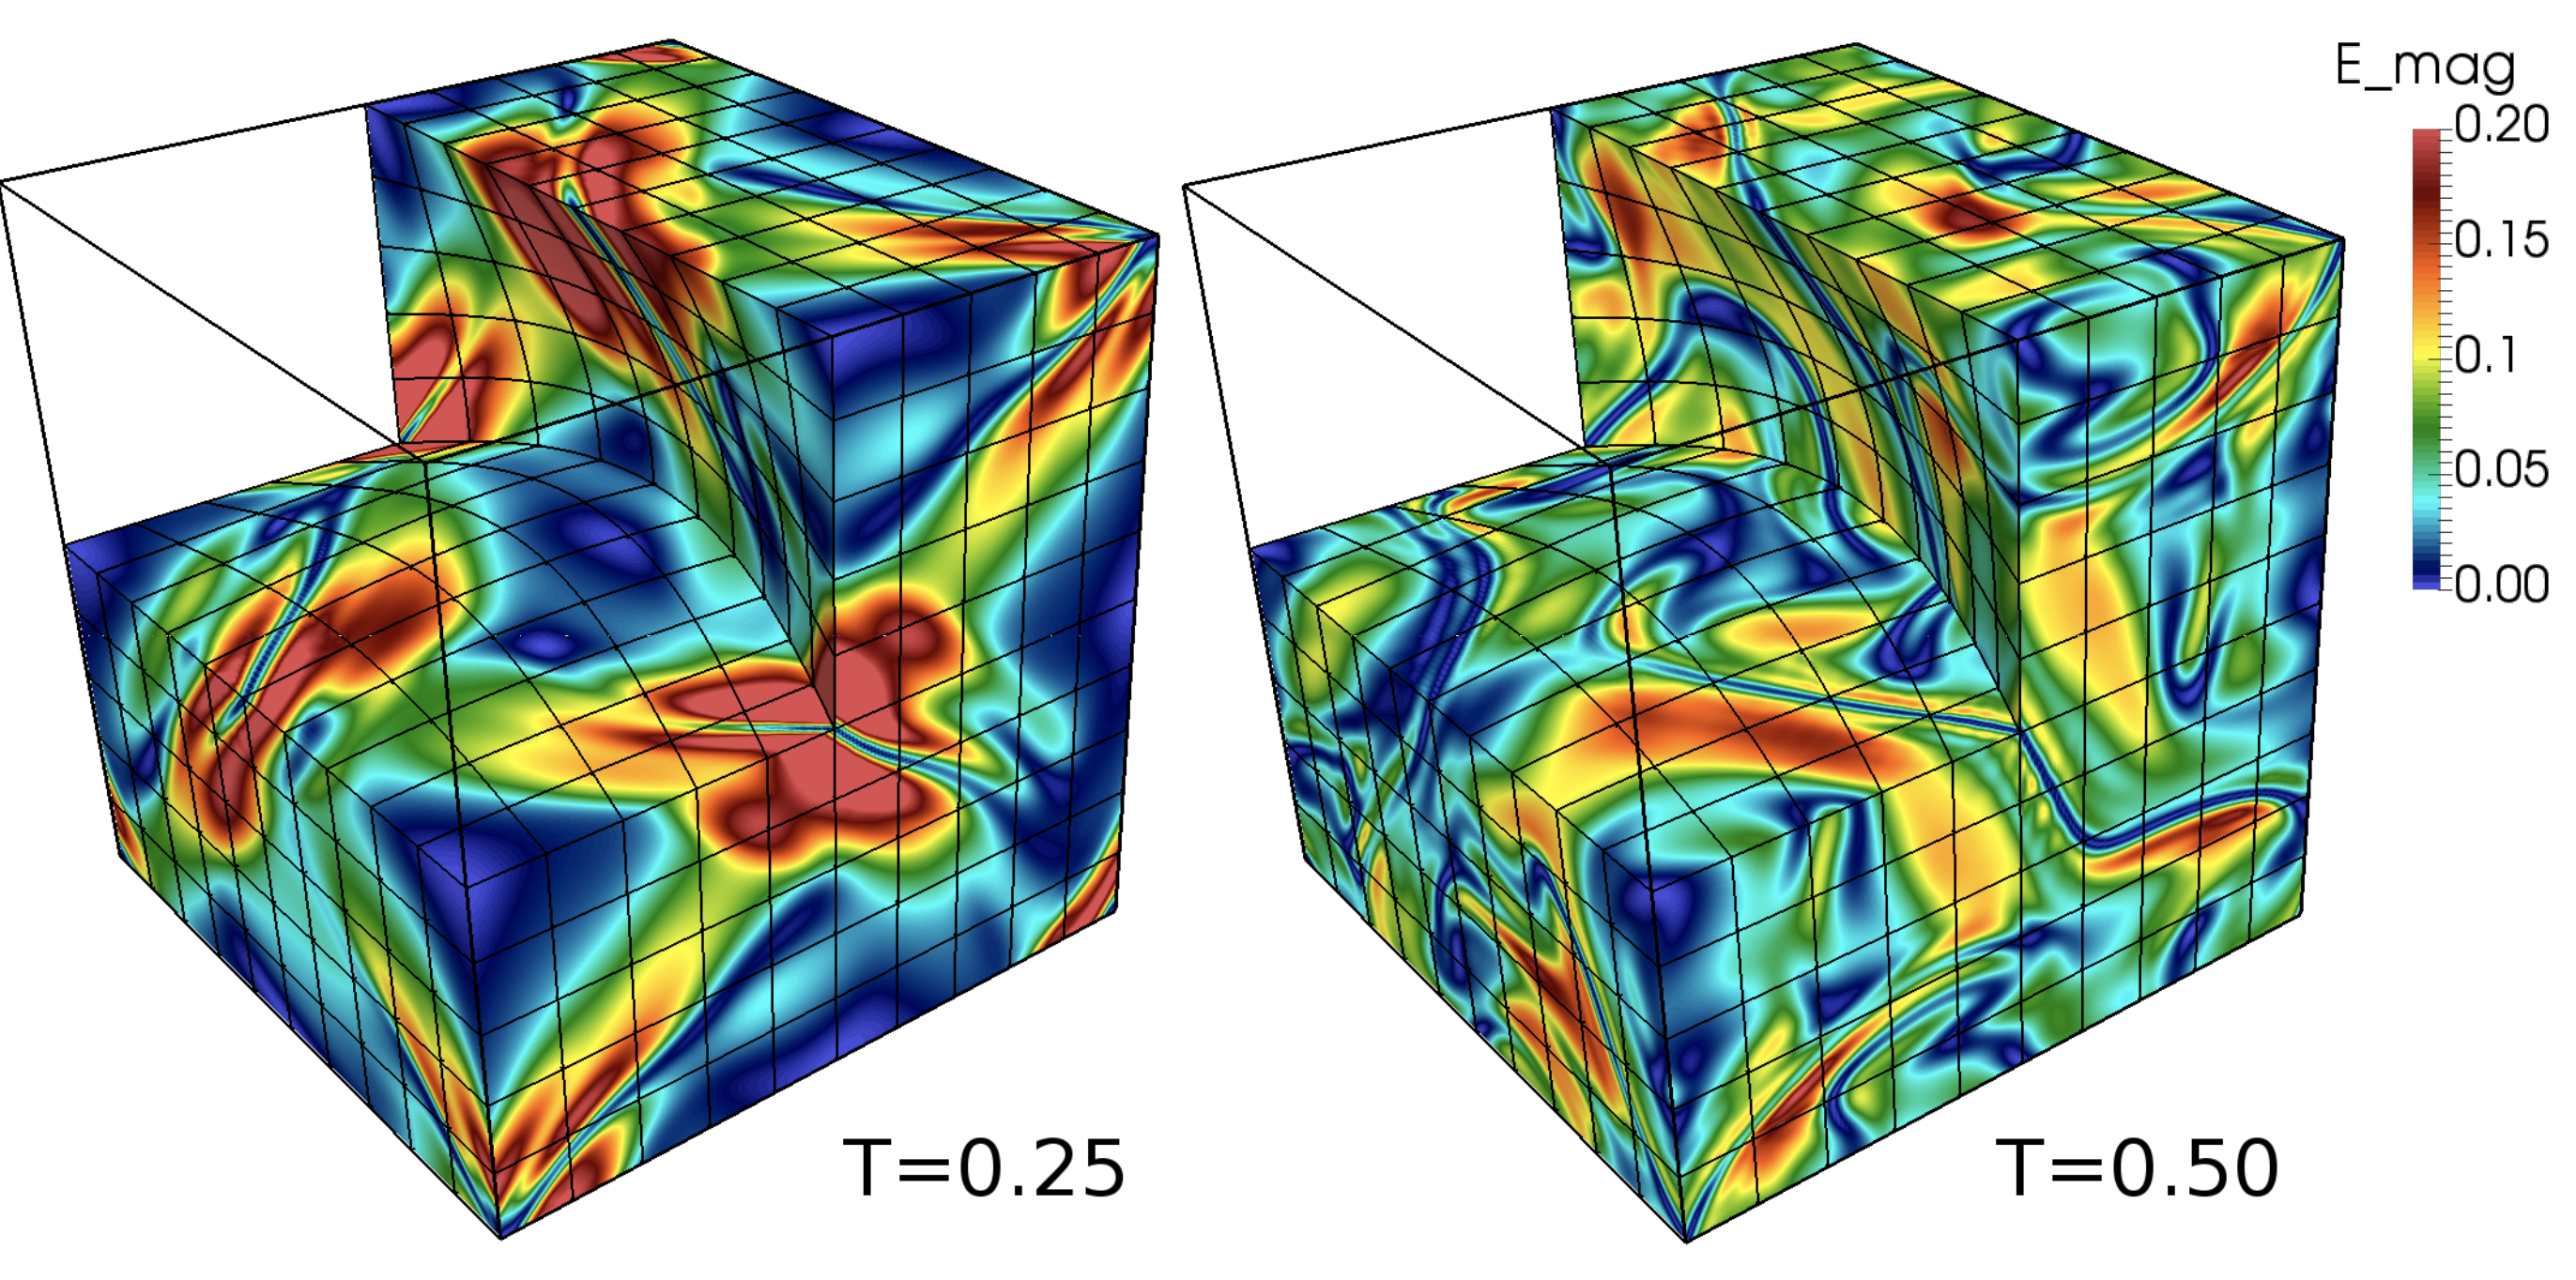
\includegraphics[width=.575\textwidth]{bohm.png}\\
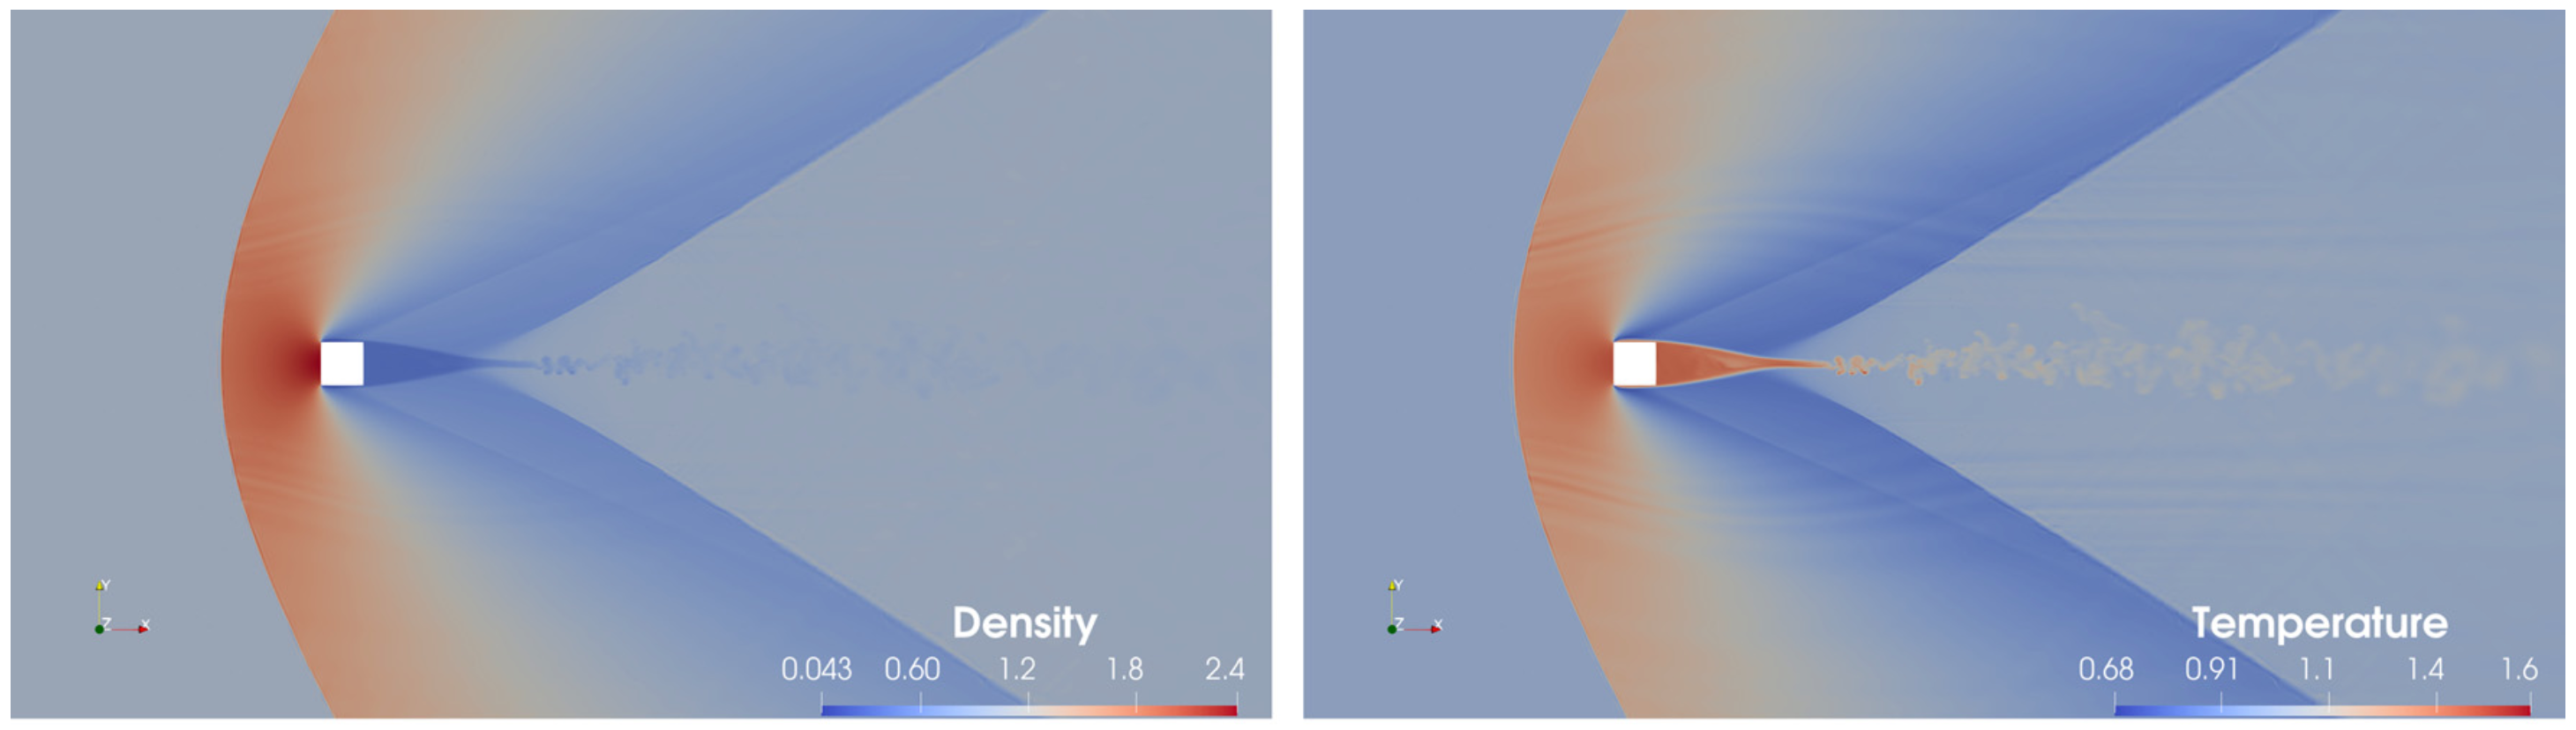
\includegraphics[width=.95\textwidth]{dalcin.png}
\end{figure}
\let\thefootnote\relax\footnotetext{\tiny Chen, Shu (2017).  \textit{Entropy stable high order DG methods with suitable quadrature rules for hyperbolic conservation laws}.}
\let\thefootnote\relax\footnotetext{\tiny Bohm et al.\ (2019).  \textit{An entropy stable nodal DG method for the resistive MHD equations. Part I}.}
\let\thefootnote\relax\footnotetext{\tiny Dalcin et al.\ (2019).  \textit{Conservative and entropy stable solid wall BCs for the compressible NS equations}.}
}

\frame{
\frametitle{Nodal DG, summation-by-parts, flux differencing}
\setcounter{subfigure}{0}

\begin{overlayarea}{\textwidth}{\textheight}
\vspace{-.25em}
\begin{figure}
\centering
\subfloat{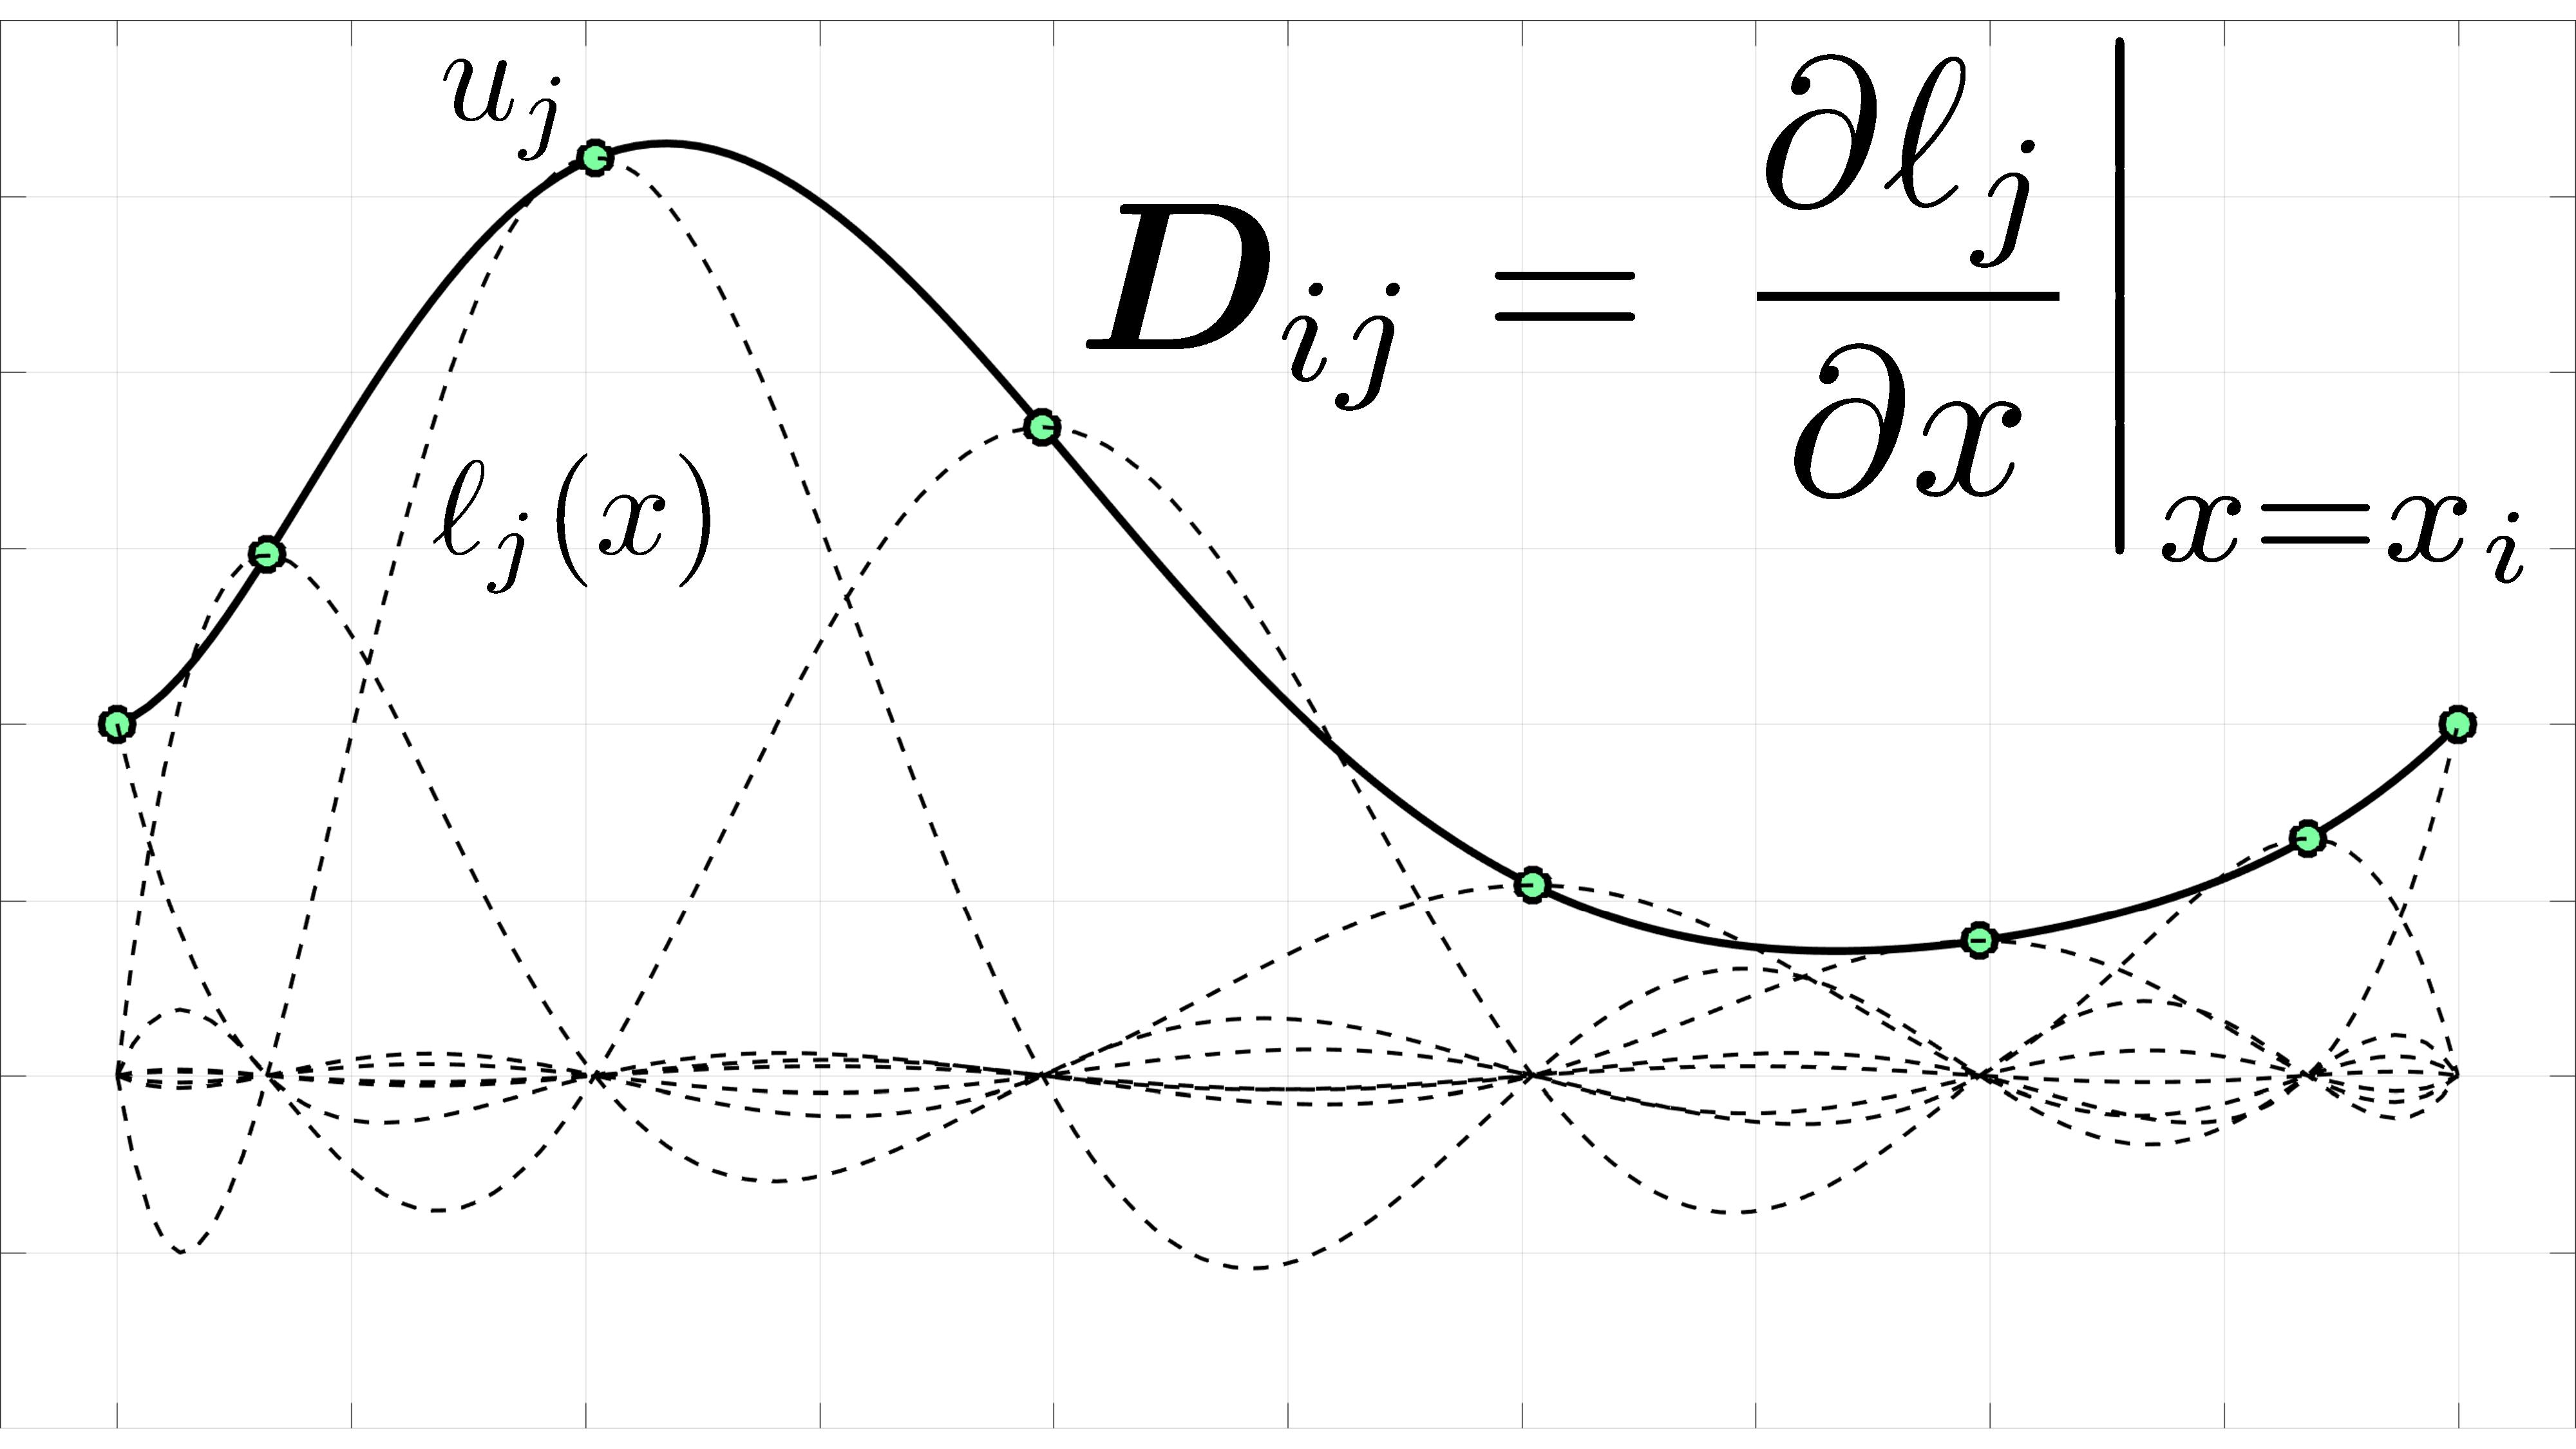
\includegraphics[width=.4\textwidth]{figs/gll1Dsbp.pdf}}
\hspace{2.5em}
\subfloat{\raisebox{.475em}{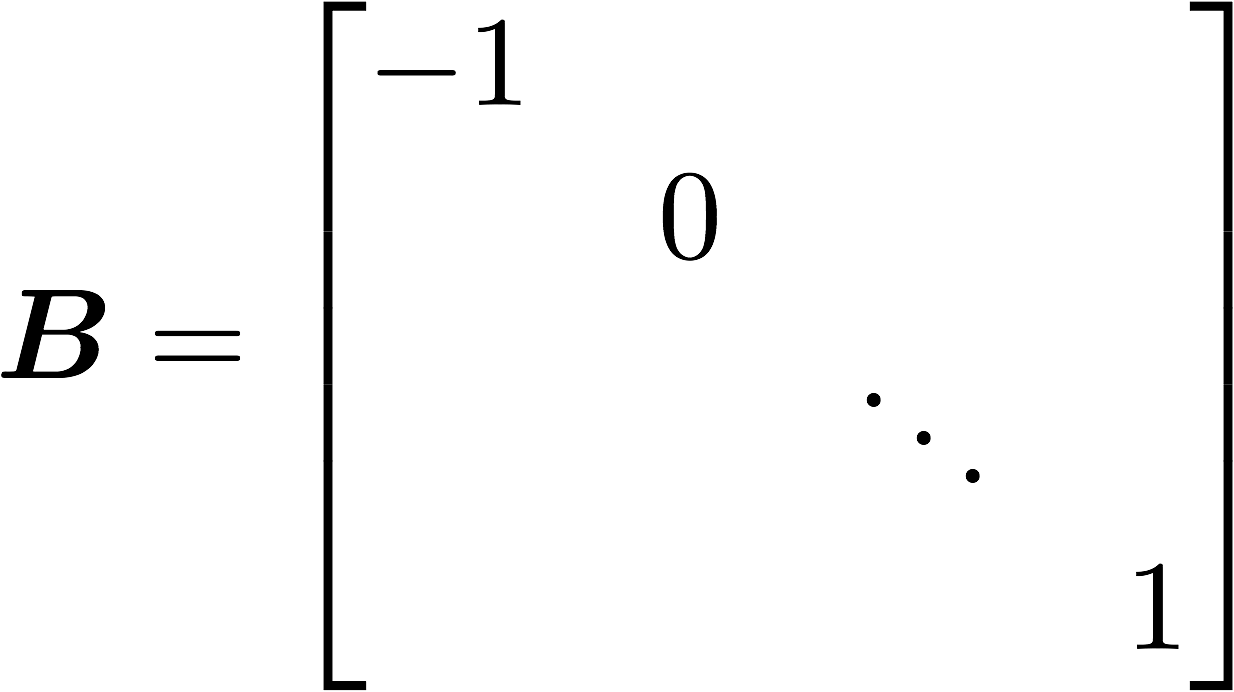
\includegraphics[width=.33\textwidth]{figs/B_SBP.png}}}
\end{figure}
\only<1>{
\begin{itemize}
\item \note{Nodal} differentiation matrix $\bm{D}$ has zero row sums
\vspace{.25em}
\[
\bm{D}\bm{1} = 0 \qquad \Longrightarrow \qquad \sum_{j} \bm{D}_{ij} = 0, \quad (\text{exact for constants})
\]
\item \note{Lobatto nodes} mimic {integration by parts} (summation-by-parts) % using differentiation matrix $\bm{D}$, diagonal (lumped) mass matrix $\bm{M}$, boundary matrix $\bm{B}$
\vspace{.25em}
\[
\bm{Q} = \bm{M}\bm{D}, \qquad \bm{M} \text{ diag.\ mass matrix}, \qquad {\boxed{\bm{Q} = \bm{B} - \bm{Q}^T}.}
\]
%\vspace{.01em}
\end{itemize}
}
\only<2->{
\vspace{-.5em}
\begin{itemize}
\item<2-> {Nodal} ``collocation'' over a single element:
\[
\int\pd{\bm{f}(\bm{u})}{x} v(x) \approx \bm{Q}\bm{f}(\bm{u})  \quad  \Longrightarrow \quad \sum_{j} \bm{Q}_{ij} \bm{f}\LRp{\bm{u}_j}.
\]
\item<2-> Let $\bm{f}_S(\bm{u}_i,\bm{u}_j) = \frac{1}{2}\LRp{\bm{f}(\bm{u}_i)+\bm{f}(\bm{u}_j)} = {\bm{F}}_{ij}$.  $\bm{Q}\bm{f}(\bm{u})$ is equivalent to
\[
\sum_{j} \bm{Q}_{ij} \bm{f}\LRp{\bm{u}_j} = \sum_{j} \bm{Q}_{ij} \note{2\bm{f}_S\LRp{\bm{u}_i,\bm{u}_j}} \quad \Longrightarrow \quad \boxed{2\LRp{\bm{Q}\circ\note{\bm{F}}}\bm{1} = 0.}
\]
\end{itemize}
}
\end{overlayarea}
}


\frame{
\frametitle{Flux differencing and entropy conservative fluxes}
\begin{itemize}
\item Applying a difference matrix $\bm{Q}$ to $\bm{f}(\bm{u})$ can be interpreted as \note{flux differencing} on a central flux 
\[
\boxed{\bm{Q}\bm{f}(\bm{u})} \Longleftrightarrow \boxed{2\LRp{\bm{Q}\circ\note{\bm{F}}}\bm{1} = 0}, \qquad \text{ if } \bm{F}_{ij} = \frac{1}{2}\LRp{\bm{f}(\bm{u}_i)+\bm{f}(\bm{u}_j)}.
\]
\vspace{.1em}
\item<2> Main idea: use Tadmor's entropy conservative numerical flux for $\bm{f}_S$
%\vspace{-.25em}
\begin{align*}
\bm{f}_S(\bm{u},\bm{u}) &= \bm{f}(\bm{u}), \qquad \text{(consistency)} \\
\bm{f}_S(\bm{u},\bm{v}) &= \bm{f}_S(\bm{v},\bm{u}),\qquad \text{(symmetry)} \\
\LRp{\bm{v}_L - \bm{v}_R}^T \bm{f}_S\LRp{\bm{u}_L,\bm{u}_R} &= \psi_L - \psi_R, \qquad \text{(conservation)}.
\end{align*}
\end{itemize}

\let\thefootnote\relax\footnotetext{\tiny Tadmor, Eitan (1987). \textit{The numerical viscosity of entropy stable schemes for systems of conservation laws. I.}}
}

\frame{
\frametitle{Entropy stable nodal DG: a brief summary}

\begin{itemize}
%\item Trick: use Tadmor's entropy conservative numerical flux for $\bm{f}_S$
%\vspace{-.25em}
%\begin{align*}
%\bm{f}_S(\bm{u},\bm{u}) &= \bm{f}(\bm{u}), \qquad \text{(consistency)} \\
%\bm{f}_S(\bm{u},\bm{v}) &= \bm{f}_S(\bm{v},\bm{u}),\qquad \text{(symmetry)} \\
%\LRp{\bm{v}_L - \bm{v}_R}^T \bm{f}_S\LRp{\bm{u}_L,\bm{u}_R} &= \psi_L - \psi_R, \qquad \text{(conservation)}.
%\end{align*}
\item<1-> If $\bm{Q}$ satisfies \note{$\bm{Q}\bm{1} = \bm{0}$} and the \note{summation-by-parts (SBP)} property, then the following (local) formulation is entropy \emph{conservative}  
\[
\boxed{\bm{M}\td{\bm{u}}{t} + 2\LRp{\bm{Q}\circ\bm{F}}\bm{1} + \bm{B}\big(\underbrace{\bm{f}_S\LRp{\bm{u}^+,\bm{u}}}_{\text{interface flux }\bm{f}^*}-\bm{f}(\bm{u})\big) = \bm{0}}
\]
\vspace{.1em}
\item<2-> Add interface dissipation (e.g., Lax-Friedrichs) for entropy \emph{stability}.
\[
\bm{f}_S\LRp{\bm{u}^+,\bm{u}}\rightarrow \bm{f}_S\LRp{\bm{u}^+,\bm{u}} - \frac{\lambda}{2} \jump{\bm{u}}, \qquad \lambda > 0. %\text{maximum wavespeed.}
\]
\end{itemize}
%\let\thefootnote\relax\footnotetext{\tiny Tadmor, Eitan (1987), Fisher and Carpenter (2014), Gassner, Winters, and Kopriva (2016).}
}

\frame{
\frametitle{Main innovation of entropy stable SBP schemes}
\vspace{-.5em}
\begin{itemize}
\item Discrete analogue of the entropy identity
\vspace{-.5em}
\begin{columns}
\begin{column}{.6\textwidth}
\centering
\begin{subequations}
\begin{empheq}[box=\fbox]{align*}
  \int_{-1}^1 \bm{v}^T\pd{\bm{f}(\bm{u})}{x}  =\LRu{\bm{v}^T\bm{f}(\bm{u}) - \psi(\bm{u})}_{-1}^1
\end{empheq}
\end{subequations}
\end{column}
$\Longleftrightarrow$
\begin{column}{.4\textwidth}
\centering
\begin{subequations}
\begin{empheq}[box=\fbox]{align*}
  \bm{v}^T&\LRp{2\bm{Q}\circ\bm{F}}\bm{1} \\
  =&\bm{1}^T\bm{B}\LRp{\bm{v}^T\bm{f}(\bm{u}) - \bm{\psi}}
\end{empheq}
\end{subequations}
\end{column}
\end{columns}
\vspace{.5em}
\item<2-> Expand $\bm{v}^T\LRp{2\bm{Q}\circ\bm{F}}\bm{1}$ using the SBP property $\bm{Q} = \bm{B}-\bm{Q}^T$
\begin{overlayarea}{\textwidth}{.135\textheight}
\[
\hspace*{-1em}
\only<1-2>{\bm{v}^T\LRp{2\bm{Q}\circ\bm{F}}\bm{1}}
\only<3>{\bm{v}^T\LRp{{\LRp{\bm{Q}-\bm{Q}^T}}\circ\bm{F}}\bm{1} + \note{\bm{v}^T\LRp{\bm{B}\circ\bm{F}}\bm{1}}, \qquad \text{(SBP property)}}
\only<4->{\bm{v}^T\LRp{\LRp{\bm{Q}-\bm{Q}^T}\circ\bm{F}}\bm{1} + \note{\bm{v}^T\bm{B} \bm{f}(\bm{u})}, \qquad \text{(consistency, $\bm{B}$ diagonal)}}
\]
\end{overlayarea}
\vspace{.1em}
\item<5-> Manipulate volume term using  properties of $\bm{Q}$ and $\bm{f}_S$.
\begin{overlayarea}{\textwidth}{.165\textheight}
\[
\only<1-5>{\bm{v}^T\LRp{\LRp{\bm{Q}-\bm{Q}^T}\circ\bm{F}}\bm{1} = \sum_{ij} \bm{Q}_{ij} \note{\LRp{\bm{v}_i-\bm{v}_j}^T \bm{f}_S\LRp{\bm{u}_i,\bm{u}_j}}}
\only<6>{\bm{v}^T\LRp{\LRp{\bm{Q}-\bm{Q}^T}\circ\bm{F}}\bm{1} =\sum_{ij} \bm{Q}_{ij} \note{\LRp{\psi(\bm{u}_i)-\psi(\bm{u}_j)}}}
\only<7>{\bm{v}^T\LRp{\LRp{\bm{Q}-\bm{Q}^T}\circ\bm{F}}\bm{1} = \bm{\psi}^T\bm{Q}\bm{1} - \bm{1}^T\bm{Q}\bm{\psi}}
\only<8>{\bm{v}^T\LRp{\LRp{\bm{Q}-\bm{Q}^T}\circ\bm{F}}\bm{1} = \underbrace{\note{\bm{\psi}^T\bm{Q}\bm{1}}}_{= \bm{0}} - \bm{1}^T\bm{Q}\bm{\psi}}
\only<9>{\bm{v}^T\LRp{\LRp{\bm{Q}-\bm{Q}^T}\circ\bm{F}}\bm{1} = \underbrace{\bm{\psi}^T\bm{Q}\bm{1}}_{= \bm{0}} - \underbrace{\note{\bm{1}^T\bm{Q}\bm{\psi}}}_{=-\bm{1}^T\bm{B}\bm{\psi}}}
\only<10>{\bm{v}^T\LRp{\LRp{\bm{Q}-\bm{Q}^T}\circ\bm{F}}\bm{1} = \note{-\bm{1}^T\bm{B}\bm{\psi}}}
%\only<11>{\bm{v}^T\LRp{2\bm{Q}\circ\bm{F}}\bm{1} = \bm{v}^T\LRp{\LRp{\bm{Q}-\bm{Q}^T}\circ\bm{F}}\bm{1} + \note{\bm{v}^T\bm{B} \bm{f}(\bm{u})}}
\]
\end{overlayarea}
\end{itemize}
\let\thefootnote\relax\footnotetext{\tiny Tadmor (1987), Carpenter et al.\ (2014), Gassner, Winters, and Kopriva (2016).}
}
%\frame{
%\frametitle{Entropy stable schemes: a brief derivation}
%
%\begin{itemize}
%\item Can derive a skew-symmetric formulation on each element:
%\[
%\bm{M}\td{\bm{u}}{t} + 2\LRp{\bm{Q}\circ\bm{F}}\bm{1} = 0
%\]
%\uncover<2->{
%\[
%\Longrightarrow \bm{M}\td{\bm{u}}{t} + \underbrace{\LRp{\LRp{\note{\bm{Q}-\bm{Q}^T}}\circ\bm{F}}\bm{1}}_{\text{SBP property}} + \LRp{\note{\bm{B}}\circ\bm{F}}\bm{1} = 0
%\]
%}
%%\uncover<3->{
%%\[
%%\Longrightarrow \bm{M}\td{\bm{u}}{t} + \LRp{\LRp{\bm{Q}-\bm{Q}^T}\circ\bm{F}}\bm{1} + \underbrace{\note{\bm{B}\bm{f}(\bm{u})}}_{\text{Consistency + diagonal } \bm{B}}  = 0.
%%\]
%%}
%\uncover<3->{
%\[
%\Longrightarrow \bm{M}\td{\bm{u}}{t} + \LRp{\LRp{\bm{Q}-\bm{Q}^T}\circ\bm{F}}\bm{1} + \underbrace{\note{\bm{B}\bm{f}^*}}_{\text{Numerical flux}}  = 0.  
%\]
%}
%\item<4-> Trick: use Tadmor's entropy conservative numerical flux for $\bm{f}_S, \bm{f}^*$
%\begin{align*}
%\bm{f}_S(\bm{u},\bm{u}) &= \bm{f}(\bm{u}), \qquad \text{(consistency)} \\
%\bm{f}_S(\bm{u},\bm{v}) &= \bm{f}_S(\bm{v},\bm{u}),\qquad \text{(symmetry)} \\
%\LRp{\bm{v}_L - \bm{v}_R}^T \bm{f}_S\LRp{\bm{u}_L,\bm{u}_R} &= \psi_L - \psi_R, \qquad \text{(conservation)}.
%\end{align*}
%%\item<6-> Proof of entropy balance: multiply by $\bm{v}^T$
%%\begin{overlayarea}{\textwidth}{.175\textheight}
%%\[
%%\hspace*{-1em}
%%\only<1-6>{\bm{v}^T\bm{M}\td{\bm{u}}{t} + \bm{v}^T\LRp{\LRp{\bm{Q}-\bm{Q}^T}\circ\bm{F}}\bm{1} + \bm{v}^T\bm{B}\bm{f}^* = 0.}
%%\only<7>{\bm{1}^T\bm{M}\td{S(\bm{u})}{t} + \sum_{ij} \bm{Q}_{ij} \note{\LRp{\bm{v}_i-\bm{v}_j}^T \bm{f}_S\LRp{\bm{u}_i,\bm{u}_j}} + \bm{v}^T\bm{B}\bm{f}^* = 0.}
%%\only<8>{\bm{1}^T\bm{M}\td{S(\bm{u})}{t} + \sum_{ij} \bm{Q}_{ij} \note{\LRp{\psi(\bm{u}_i)-\psi(\bm{u}_j)}} + \bm{v}^T\bm{B}\bm{f}^* = 0.}
%%\only<9>{\bm{1}^T\bm{M}\td{S(\bm{u})}{t} + \note{\bm{\psi}^T\bm{Q}\bm{1} - \bm{1}^T\bm{Q}\bm{\psi}} + \bm{v}^T\bm{B}\bm{f}^* = 0.}
%%\only<10>{\bm{1}^T\bm{M}\td{S(\bm{u})}{t} + \bm{1}^T\bm{B}\LRp{\bm{v}^T\bm{f}^* - \bm{\psi}}  = 0.}
%%\only<11>{\bm{1}^T\bm{M}\td{S(\bm{u})}{t} + \bm{1}^T\bm{B}\LRp{\bm{v}^T\bm{f}^* - \bm{\psi}}  \leq 0 \text{ \note{(if dissipation added)}}.}
%%\]
%%\end{overlayarea}
%\end{itemize}
%%\let\thefootnote\relax\footnotetext{\tiny Tadmor, Eitan (1987), Fisher and Carpenter (2014), Gassner, Winters, and Kopriva (2016).}
%}





%\frame{
%\frametitle{Deriving entropy stable schemes}
%
%\begin{itemize}
%\item<1-> Derive formulation with boundary (interface) flux $\bm{f}^*$
%\begin{overlayarea}{\textwidth}{.17\textheight}
%\vspace{-1em}
%\begin{align*}
%\only<1>{\bm{M}\td{\bm{u}}{t} + 2\LRp{\bm{Q}\circ\bm{F}}\bm{1} = 0}
%\only<2>{\bm{M}\td{\bm{u}}{t} + \underbrace{\LRp{\LRp{\note{\bm{Q}-\bm{Q}^T}}\circ\bm{F}}\bm{1}}_{\text{SBP property}} + \LRp{\note{\bm{B}}\circ\bm{F}}\bm{1} = 0}
%\only<3>{\bm{M}\td{\bm{u}}{t} + \LRp{\LRp{\bm{Q}-\bm{Q}^T}\circ\bm{F}}\bm{1} + \underbrace{\note{\bm{B}\bm{f}(\bm{u})}}_{\LRp{\bm{F}}_{ii} = \bm{f}(\bm{u}_i) \text{ + diagonal } \bm{B}}  = 0.}
%\only<4>{\bm{M}\td{\bm{u}}{t} + \LRp{\LRp{\bm{Q}-\bm{Q}^T}\circ\bm{F}}\bm{1} + \underbrace{\note{\bm{B}\bm{f}^*}}_{\text{Numerical flux}} = 0.  }
%\only<5->{\bm{M}\td{\bm{u}}{t} + \LRp{\LRp{\bm{Q}-\bm{Q}^T}\circ\bm{F}}\bm{1} + \bm{B}\bm{f}^* = 0.  }
%\end{align*}
%\end{overlayarea}
%\item<6-> Trick: use Tadmor's entropy conservative numerical flux for $\bm{f}_S, \bm{f}^*$
%\begin{align*}
%\bm{f}_S(\bm{u},\bm{u}) &= \bm{f}(\bm{u}), \qquad \text{(consistency)} \\
%\bm{f}_S(\bm{u},\bm{v}) &= \bm{f}_S(\bm{v},\bm{u}),\qquad \text{(symmetry)} \\
%\LRp{\bm{v}_L - \bm{v}_R}^T \bm{f}_S\LRp{\bm{u}_L,\bm{u}_R} &= \psi_L - \psi_R, \qquad \text{(conservation)}.
%\end{align*}
%\item<7-> Entropy \note{conservation}: multiply by $\bm{v}(\bm{u})^T$, chain rule in time
%\begin{overlayarea}{\textwidth}{.175\textheight}
%\[
%\hspace*{-1em}
%\only<1-7>{\bm{v}^T\bm{M}\td{\bm{u}}{t} + \bm{v}^T\LRp{\LRp{\bm{Q}-\bm{Q}^T}\circ\bm{F}}\bm{1} + \bm{v}^T\bm{B}\bm{f}^* = 0.}
%\only<8>{\bm{1}^T\bm{M}\td{S(\bm{u})}{t} + \sum_{ij} \bm{Q}_{ij} \note{\LRp{\bm{v}_i-\bm{v}_j}^T \bm{f}_S\LRp{\bm{u}_i,\bm{u}_j}} + \bm{v}^T\bm{B}\bm{f}^* = 0.}
%\only<9>{\bm{1}^T\bm{M}\td{S(\bm{u})}{t} + \sum_{ij} \bm{Q}_{ij} \note{\LRp{\psi(\bm{u}_i)-\psi(\bm{u}_j)}} + \bm{v}^T\bm{B}\bm{f}^* = 0.}
%\only<10>{\bm{1}^T\bm{M}\td{S(\bm{u})}{t} + \note{\bm{\psi}^T\bm{Q}\bm{1} - \bm{1}^T\bm{Q}\bm{\psi}} + \bm{v}^T\bm{B}\bm{f}^* = 0.}
%\only<11>{\bm{1}^T\bm{M}\td{S(\bm{u})}{t} + \bm{1}^T\bm{B}\LRp{\bm{v}^T\bm{f}^* - \bm{\psi}}  = 0.}
%\only<12>{\bm{1}^T\bm{M}\td{S(\bm{u})}{t}  = 0, \qquad \text{(for periodic domains)}.}
%\]
%\end{overlayarea}
%\end{itemize}
%\let\thefootnote\relax\footnotetext{\tiny Tadmor, Eitan (1987), Gassner, Winters, and Kopriva (2016).}
%}
%
%\frame{
%\frametitle{Example: entropy stability for Burgers' equation }
%\setcounter{subfigure}{0}
%
%\begin{figure}
%\begin{overlayarea}{\textwidth}{.5\textheight}
%%\begin{overprint}
%\centering
%\foreach \id in {1,2,3,4,5,6,7,8}{%
%\only<\id>{
%\subfloat[Energy conservative ($\tau = 0$)]{\includegraphics[width=.425\textwidth]{figs/burgersStableEC_\id.png}}\hspace{2em}%
%\subfloat[Energy stable ($\tau = 1$)]{\includegraphics[width=.425\textwidth]{figs/burgersStableLF_\id.png}}
%}% \only
%}% for
%\only<9>{
%\captionsetup[subfloat]{width=.45\textwidth, justification=centering}
%\subfloat[Entropy over time for $\tau = 0$]{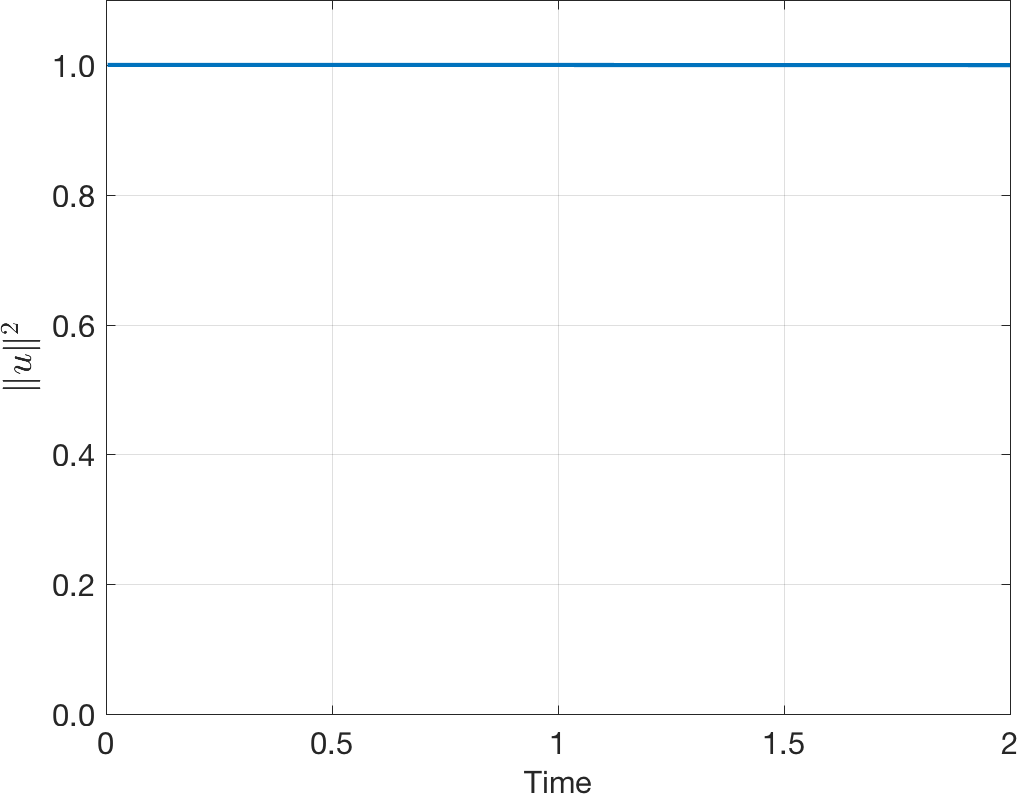
\includegraphics[width=.45\textwidth]{figs/burgersSplitEnergyEC.png}}\hspace{1em}%
%\subfloat[Entropy over time for $\tau = 1$]{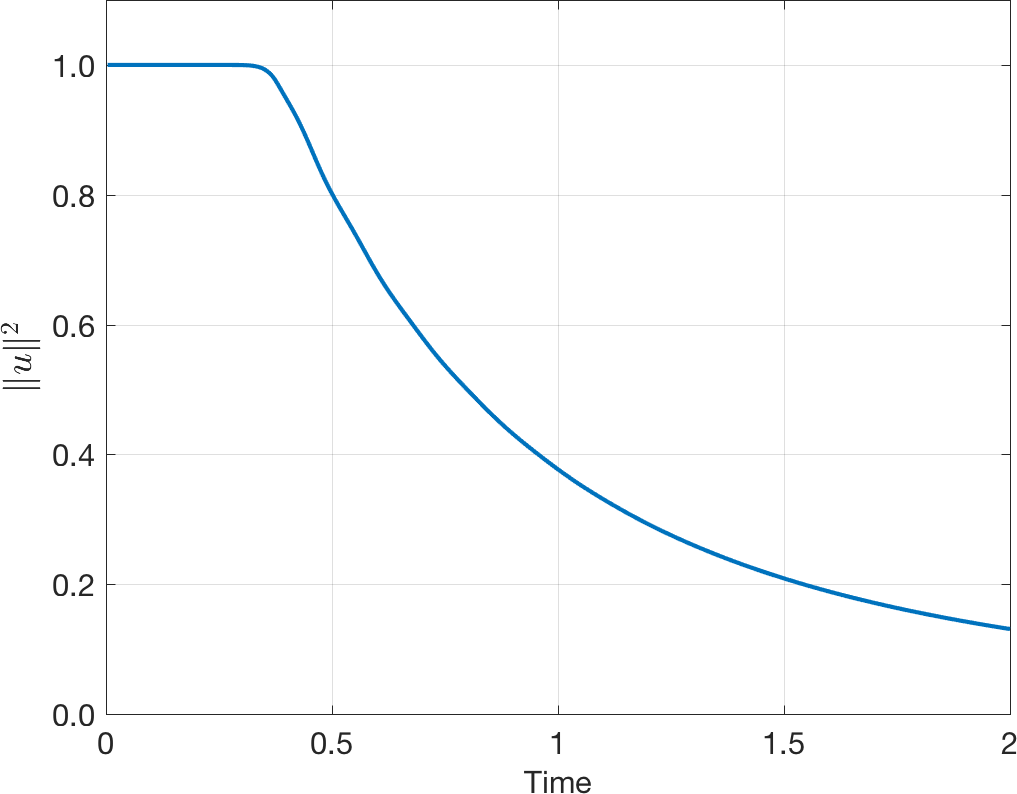
\includegraphics[width=.45\textwidth]{figs/burgersSplitEnergyLF.png}}
%}
%%\end{overprint}
%\end{overlayarea}
%\vspace{1em}
%\[
%\boxed{\pd{u}{t} + \frac{1}{2}\pd{u^2}{x} = 0, \qquad S(u) = \frac{u^2}{2}.}
%\]
%\end{figure}
%}
%
%\frame{
%\frametitle{What is flux differencing doing?}
%\begin{itemize}
%\item<1-> Entropy conservative flux for Burgers' equation 
%\[
%f_S(u_L,u_R) = \frac{1}{6}\LRp{u_L^2 + u_Lu_R + u_R^2}, \qquad f_S(u,u) = f(u) = \frac{u^2}{2}.
%\]
%\item<1-> Flux differencing: let $u_L = u(x), u_R = u(y)$
%\[
%%\only<1->{\pd{{f}({u})}{x} \Longrightarrow \pd{f(u)}{u} \pd{u}{x}}
%%\only<2->{\pd{{f}({u})}{x} \Longrightarrow \pd{f_S(u,u)}{u}\pd{u}{x}}
%%\only<1->{
%\pd{{f}({u})}{x} \Longrightarrow \note{\LRu{2\pd{f_S\LRp{u(x),u(y)}}{x}}_{y=x}}
%%}
%\]
%\item<2-> Recovers a known stable split form of Burgers' equation
%\begin{gather*}
%f_S(u(x),u(y)) = \frac{1}{6}\LRp{u(x)^2 + u(x)u(y) + u(y)^2}\\
%\LRu{2\pd{f_S\LRp{u(x),u(y)}}{x}}_{y=x} = \frac{1}{3}\pd{u^2}{x} + \frac{1}{3}u\pd{u}{x} + \frac{1}{3}u^2\cancel{\pd{1}{x}}.
%\end{gather*}
%\end{itemize}
%}
%
%%\frame{
%%\frametitle{Flux differencing: beyond split formulations}
%%\begin{itemize}
%%\item Fluxes $\bm{f}_S$ do not necessarily correspond to split formulations!  
%%\vspace{.5em}
%%\item Example: entropy conservative flux for 1D compressible Euler
%%\begin{align*}
%%f^1_S(\bm{u}_L,\bm{u}_R) &= \avg{\rho}^{\log} \avg{u}\\
%%f^2_S(\bm{u}_L,\bm{u}_R) &= \frac{\avg{\rho}}{2\avg{\beta}} + \avg{u}f^1_S\\
%%f^3_S(\bm{u}_L,\bm{u}_R) &= f^1_S\LRp{\frac{1}{2(\gamma-1)\avg{\beta}^{\log}} - \frac{1}{2}\avg{u^2}} + \avg{u}f^2_S,
%%\end{align*}
%%%\vspace{.5em}
%%\item Rational functions: logarithmic mean and ``inverse temperature'' $\beta$
%%\[
%%\avg{u}^{\log} = \frac{u_L - u_R}{\log{u_L}- \log{u_R}}, \qquad \beta = \frac{\rho}{2p}.
%%\]
%%\end{itemize}
%%
%%\let\thefootnote\relax\footnotetext{\tiny Chandreshekar (2013),  \emph{Kinetic energy preserving and entropy stable FV schemes for comp.\ Euler and NS equations.}}
%%}
%%
%
%\frame{
%\frametitle{Beyond split formulations: compressible Euler}
%\vspace{-.5em}
%\begin{figure}
%\centering
%\begin{overlayarea}{\textwidth}{.4\textheight}
%\only<1>{
%\subfloat[Entropy conservative flux, $T = .3$]{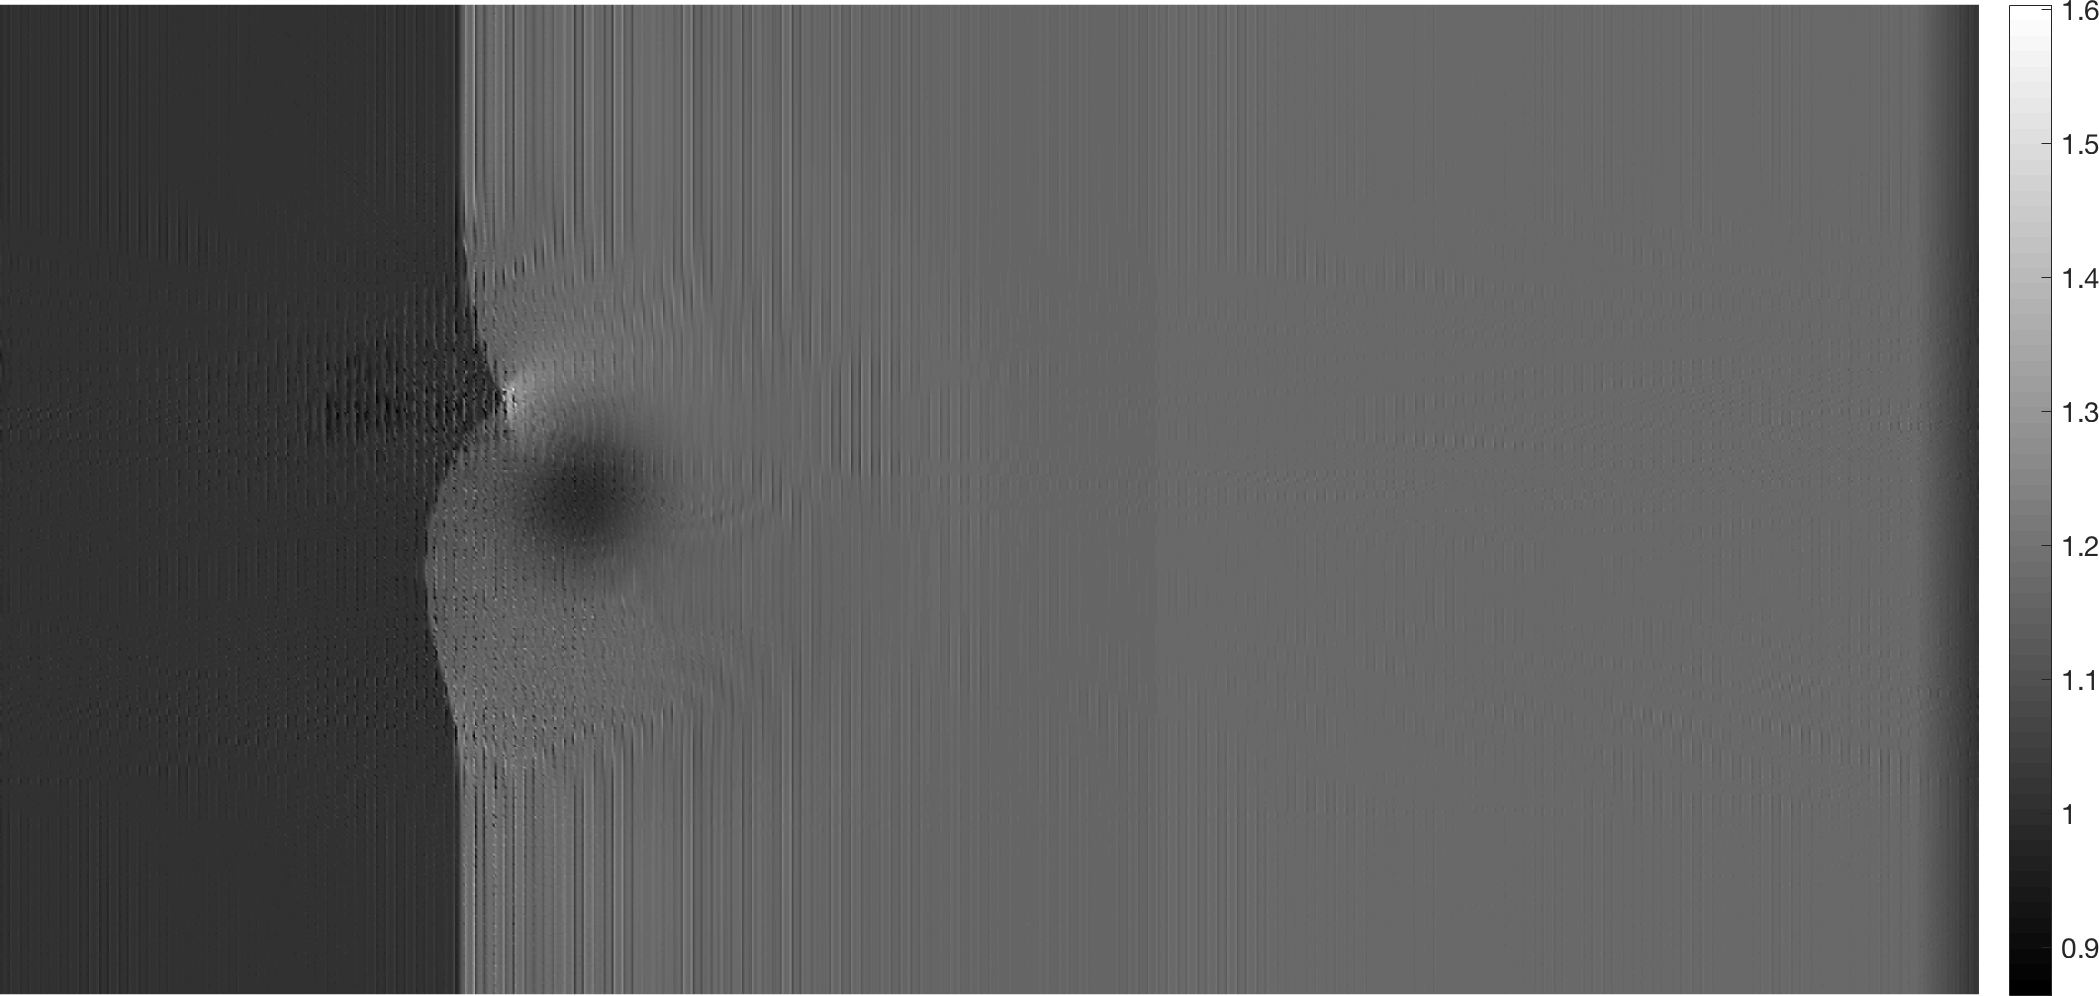
\includegraphics[width=.49\textwidth]{figs/shockVortexTp3_EC.png}}
%\hspace{.05em}
%\subfloat[Entropy conservative flux, $T = .7$]{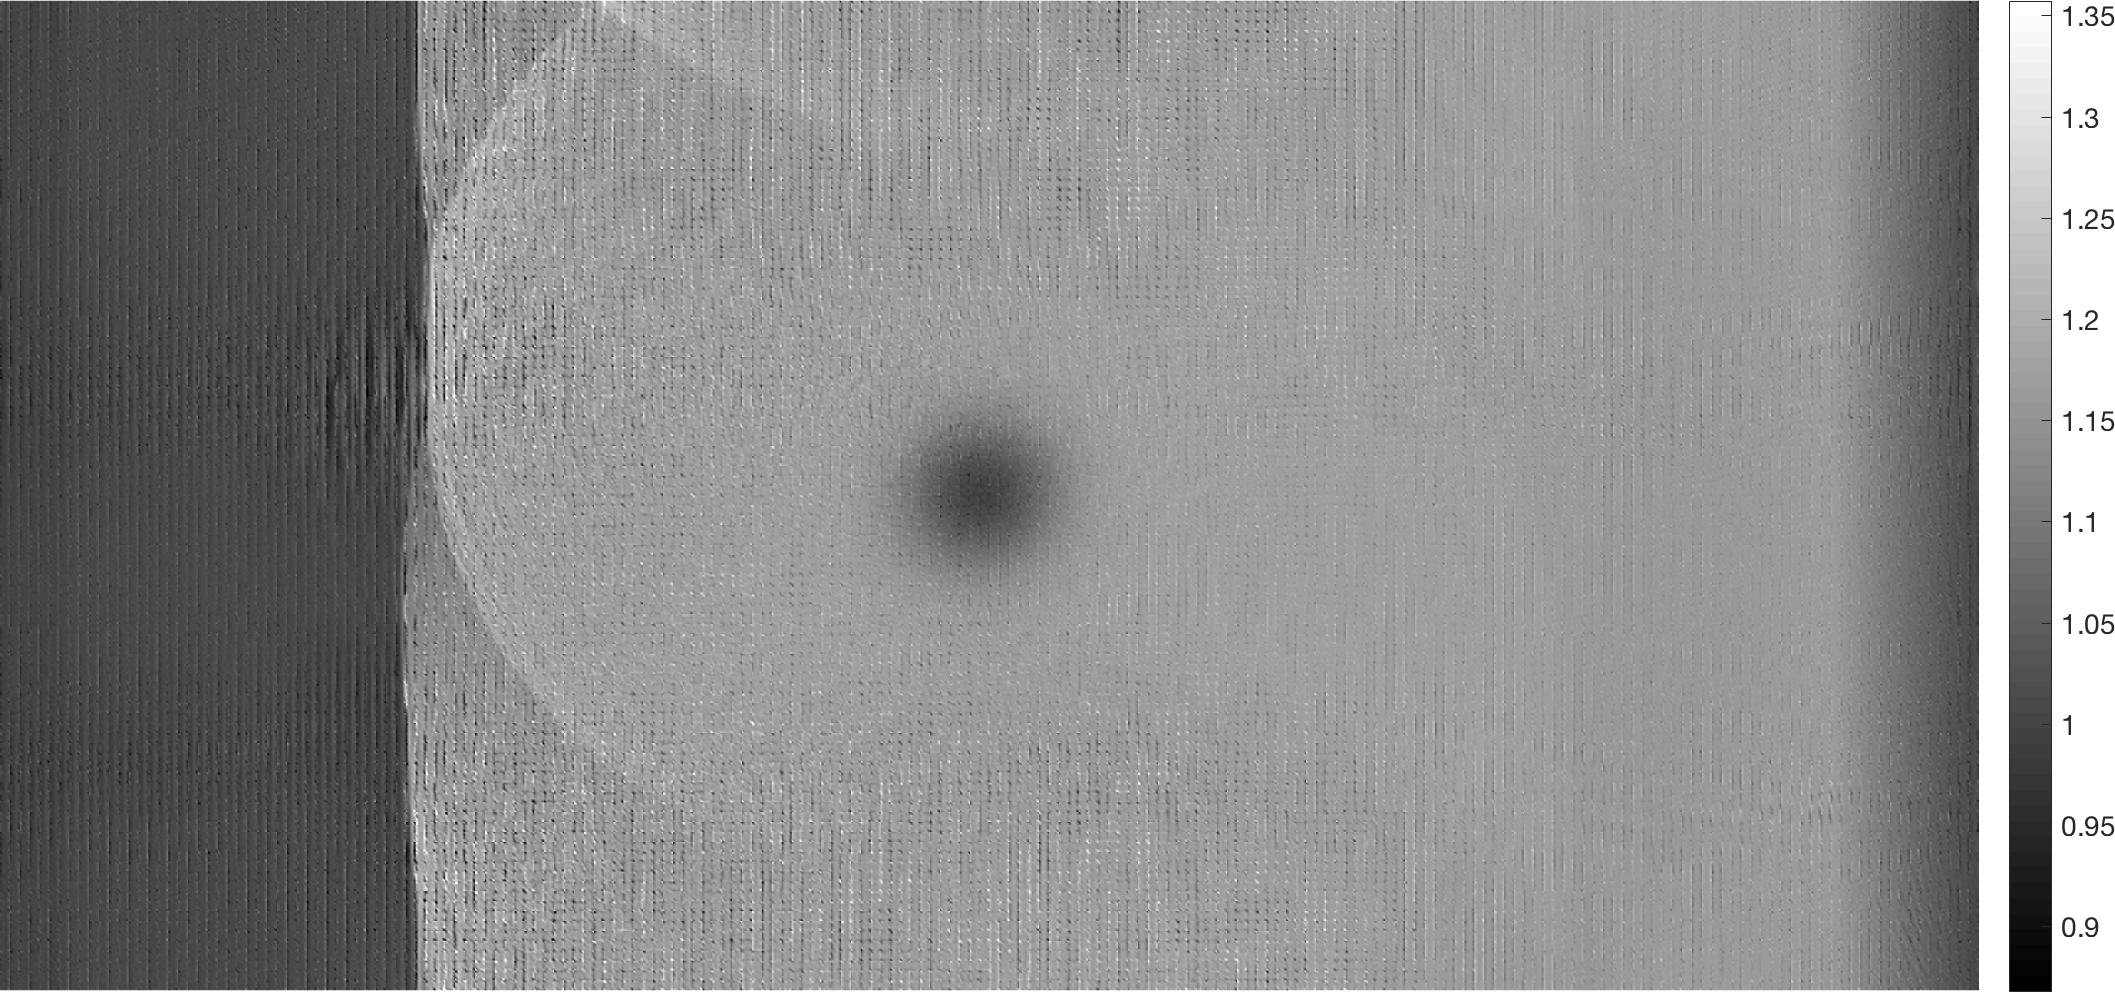
\includegraphics[width=.49\textwidth]{figs/shockVortexTp7_EC.png}}
%}
%\only<2>{
%\subfloat[Local Lax-Friedrichs flux, $T = .3$]{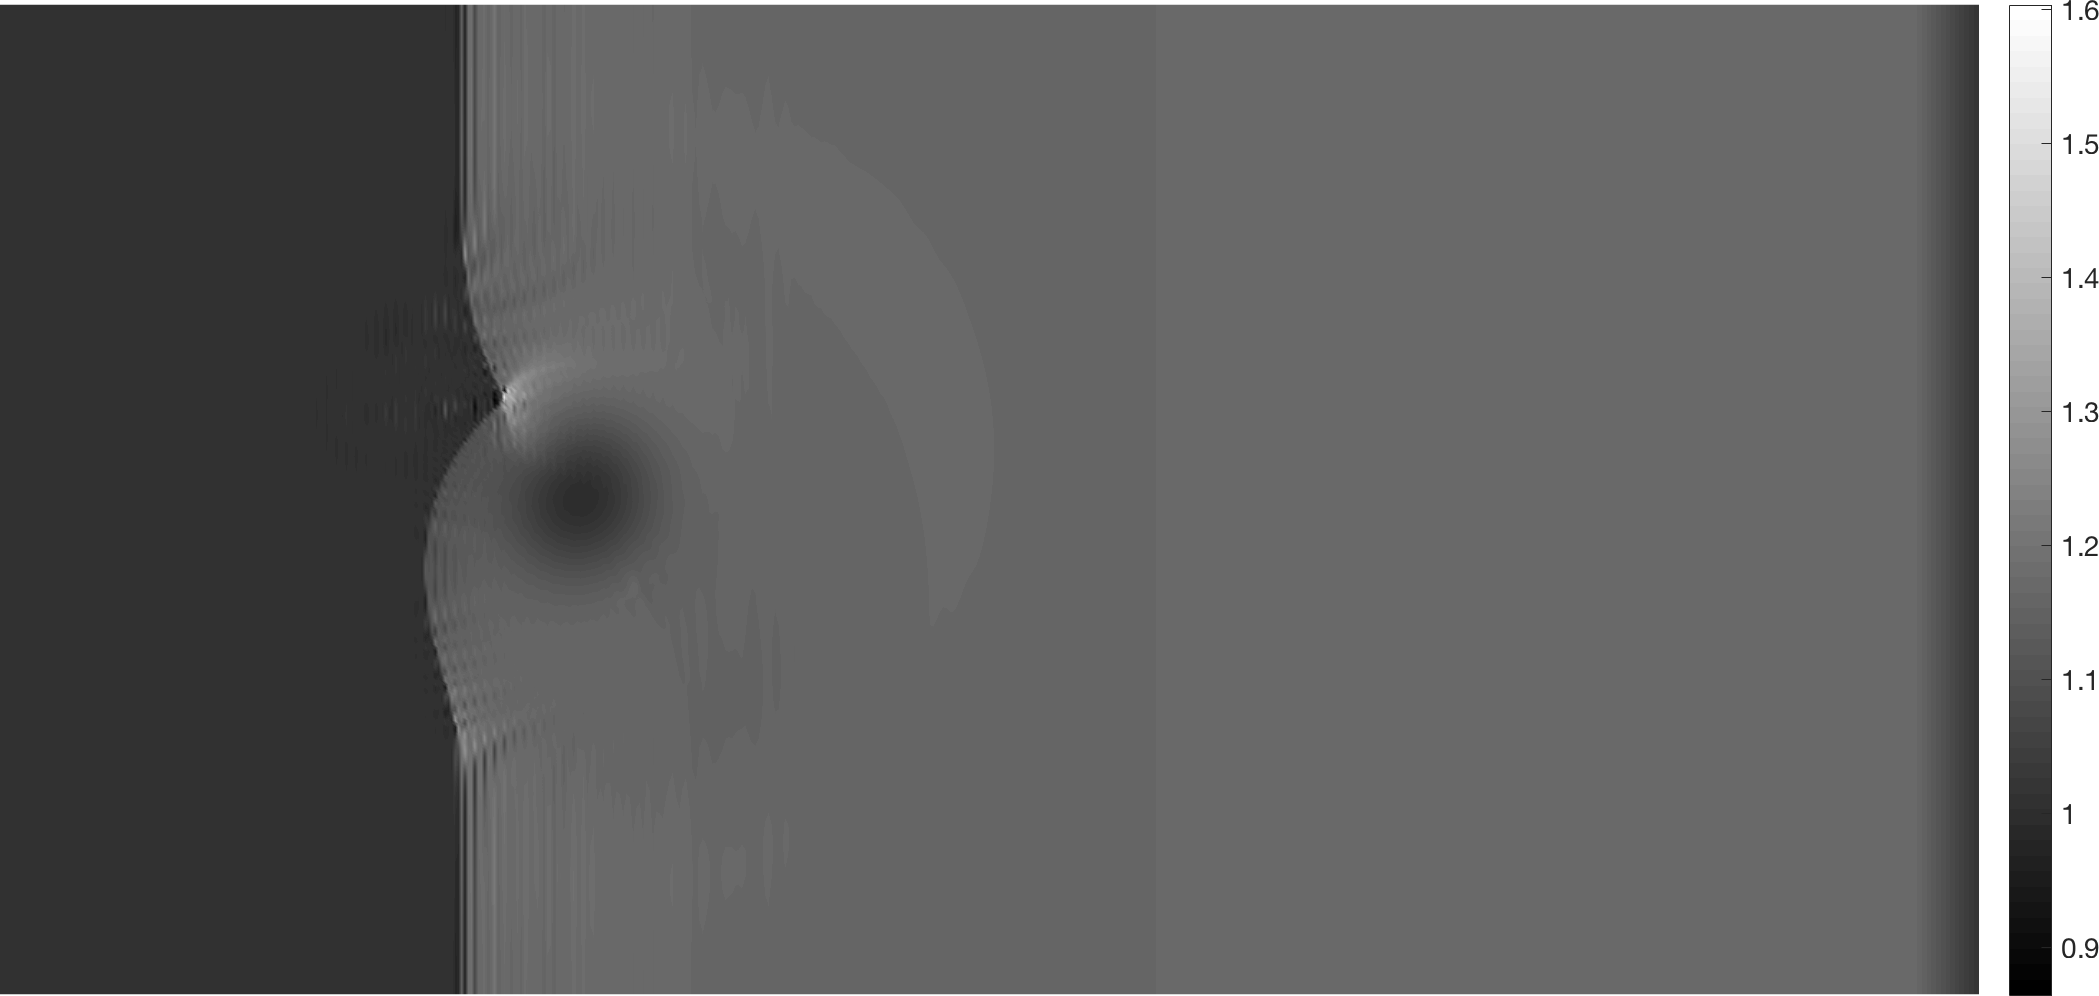
\includegraphics[width=.49\textwidth]{figs/shockVortexTp3_LF.png}}
%\hspace{.05em}
%\subfloat[Local Lax-Friedrichs flux, $T = .7$]{\includegraphics[width=.49\textwidth]{figs/shockVortexTp7_LF.png}}\
%}
%\only<3>{
%\subfloat[Matrix dissipation flux, $T = .3$]{\includegraphics[width=.49\textwidth]{figs/shockVortexTp3.png}}
%\hspace{.05em}
%\subfloat[Matrix dissipation flux, $T = .7$]{\includegraphics[width=.49\textwidth]{figs/shockVortexTp7.png}}
%}
%\only<4>{
%\subfloat[Matrix dissipation flux, $T = .3$]{\includegraphics[width=.485\textwidth]{figs/shockVortexT3.png}}
%\hspace{.05em}
%\subfloat[Matrix dissipation flux, $T = .7$]{\includegraphics[width=.49\textwidth]{figs/shockVortexT7.png}}
%}
%\end{overlayarea}
%\caption{\footnotesize Compressible Euler shock vortex interaction: $200\times 100$ \note{degree $N=4$} elements, $4$th order \note{explicit} RK time-stepping, no limiters or artificial viscosity.  }
%\label{fig:shockvort}
%\end{figure}
%
%Fluxes $\bm{f}_S$ \note{rational} in general (compressible Euler uses logarithmic mean).
%\[
%\avg{u}^{\log} = \frac{u_L - u_R}{\log{u_L}- \log{u_R}}
%\]
%
%\let\thefootnote\relax\footnotetext{\tiny Jiang, Shu (1998).  \textit{Efficient Implementation of Weighted ENO Schemes}.}
%\let\thefootnote\relax\footnotetext{\tiny Chandrashekar (2013). \textit{Kinetic energy preserving and entropy stable FV schemes for compressible Euler and NS equations.}}
%\let\thefootnote\relax\footnotetext{\tiny Winters, Derigs, Gassner, and Walch (2017). \textit{A uniquely defined entropy stable matrix dissipation operator \ldots}.}
%}

\section{Modal entropy stable DG formulations}
\frame[noframenumbering]{
\frametitle{Talk outline}
\tableofcontents[currentsection]
}

\frame{
\frametitle{Why ``modal'' formulations?}

\fbox{\begin{minipage}{.95\textwidth}
\begin{center}
Nodal formulations: tied to a specific polynomial quadrature rule.\\
\textbf{``Modal''} formulations: designed for arbitrary bases and quadratures.
\end{center}
\end{minipage}}
\vspace{1em}
\begin{itemize}
\item<2-> Nodal formulations typically \emph{underintegrate}.   \note{More accurate quadrature} reduces aliasing for nonlinear terms + curved elements.
\vspace{1em}
\item<3-> Accomodate non-polynomial \note{basis functions}: 
\begin{itemize}
\item Pyramid elements, physical-frame bases, splines
\item Projection-based \note{reduced order modeling}
\end{itemize}
\vspace{1em}
\item<4-> Extensions of (and connections with) traditional SBP operators.
\end{itemize}
\uncover<3->{
\let\thefootnote\relax\footnotetext{\tiny Bergot, Cohen, and Durufl\'{e} (2010). \textit{Higher-order finite elements for hybrid meshes using new nodal pyramidal elements.} }
\let\thefootnote\relax\footnotetext{\tiny Bassi, Botti, and Colombo (2014). \textit{Agglomeration-based physical frame dG discretizations: an attempt to be mesh free.} }
%\let\thefootnote\relax\footnotetext{\tiny Banks and Hagstrom (2016). \textit{On Galerkin difference methods.} }
\let\thefootnote\relax\footnotetext{\tiny Chan and Evans (2018). \textit{Multi-patch DG-IGA for wave propagation}. }
}
\uncover<3->{
\let\thefootnote\relax\footnotetext{\tiny Hicken, Fernandez, and Zingg (2016). \textit{Multidimensional Summation-By-Parts Operators\ldots}}
}
}

%\frame{
%\frametitle{Applications of ``modal'' vs nodal DG methods}
%\setcounter{subfigure}{0}
%\vspace{-.75em}
%\begin{figure}
%\centering
%\only<1>{
%\subfloat[Lobatto nodal DG]{\raisebox{.25em}{\includegraphics[width=.25\textwidth]{figs/SEM_stencil_1.pdf}}}
%}
%\only<2->{\visible<2->{\setcounter{subfigure}{0}\subfloat[Gauss nodes]{\raisebox{.25em}{\includegraphics[width=.2\textwidth]{figs/gsbp.png}}}}
%\hspace{.25em}
%\visible<3->{\subfloat[Non-conforming meshes]{\includegraphics[width=.4\textwidth]{figs/nonconQuad.pdf}}}
%%\hspace{.25em}
%\visible<4->{\subfloat[Hybrid meshes]{\includegraphics[width=.31\textwidth]{figs/hybrid3D.png}}}
%}
%\end{figure}
%\vspace{-.25em}
%\begin{itemize}
%\item<1-> Goal: generalize entropy stability beyond nodal DG to ``modal'' DG (arbitrary choices of basis and quadrature).  
%\vspace{.25em}
%\item<2-> Avoid restrictions on quadrature (boundary points, ``collocation''), and basis (pyramids, reduced order modeling)
%\end{itemize}
%
%
%\visible<5>{
%\begin{center}
%\minibox[frame]{Goal: extend \note{entropy stability} to high order modal DG formulations.}
%\end{center}
%}
%%\let\thefootnote\relax\footnotetext{\tiny Fisher and Carpenter (2013). \textit{High-order ES finite difference schemes for nonlinear conservation laws: Finite domains.} }
%%\let\thefootnote\relax\footnotetext{\tiny Gassner, Winters, and Kopriva (2016). \textit{Split form nodal DG schemes with SBP property for the comp.\ Euler equations.}}
%%\let\thefootnote\relax\footnotetext{\tiny Carpenter et al.\ (2014). \textit{Entropy stable spectral collocation schemes for the NS equations: discontinuous interfaces.}}
%\let\thefootnote\relax\footnotetext{\tiny Carpenter et al.\ (2014), Gassner, Winters, and Kopriva (2016), Hicken et al.\ (2016), Crean et al.\ (2018)}
%\let\thefootnote\relax\footnotetext{\tiny Bergot, Cohen, Durufl\'{e} (2010). \textit{Higher-order finite elements for hybrid meshes using new nodal pyramidal elements.}}
%}

\frame{
\frametitle{Challenges for modal formulations}
\vspace{-.5em}
\begin{itemize}
\item Challenge 1: entropy variables are not contained in the finite element test space!  If $\bm{u}\in P^N$, then in general, $\bm{v}(\bm{u}) \not\in P^N$.  
\vspace{1.5em}
\item Challenge 2: inter-element coupling more complicated and expensive.
\end{itemize}
%\vspace{-.5em}
\begin{figure}
\centering
\begin{overlayarea}{.525\textwidth}{.4\textheight}
\only<1>{\includegraphics[width=\textwidth]{dg_coupling.png}\caption*{\footnotesize Standard DG coupling (through face points)}}
\only<2>{\includegraphics[width=\textwidth]{gsbp_coupling.png}\caption*{\footnotesize Entropy stable DG coupling (all-to-all)}}
\end{overlayarea}
\end{figure}
}

\frame{
\frametitle{Challenge 1: entropy projection}

\begin{itemize}
\item DG: cannot test with entropy variables, only with polynomials.
\vspace{1em}
\item<2-> Let $\bm{u}_N$ be a polynomial.  
%Use $L^2$ projection of entropy variables 
%\[
%\int_{D^k} P_N \bm{v}\LRp{\bm{u}_N} \bm{w} = \int_{D^k} \bm{v}\LRp{\bm{u}_N} \bm{w}, \qquad \forall \bm{w}\in \LRp{P^N}^d. 
%\]
%\item 
Testing with the \note{$L^2$ projection of the entropy variables} $P_N \bm{v}\LRp{\bm{u}_N}$ recovers evolution of entropy
\[
\int_{D^k} P_N \bm{v}\LRp{\bm{u}_N}^T\pd{\bm{u}_N}{t} = \int_{D^k} \underbrace{\bm{v}\LRp{\bm{u}_N}^T}_{\pd{S(\bm{u})}{\bm{u}}}\pd{\bm{u}_N}{t}  =  \int_{D^k}\pd{S(\bm{u}_N)}{t} 
\]
\vspace{.01em}
\item<3-> For consistency with the test function $P_N \bm{v}\LRp{\bm{u}_N}$, spatial formulation is evaluated using projected entropy variables $\tilde{\bm{u}} = \bm{u}\LRp{P_N \bm{v}\LRp{\bm{u}_N}}$.  
\[
\LRp{\bm{v}_i-\bm{v}_j}^T \bm{f}_S\LRp{\bm{u}_i,\bm{u}_j} \neq {\psi(\bm{u}_i)-\psi(\bm{u}_j)} \quad \text{if  } \bm{v}_i \neq \bm{v}\LRp{\bm{u}_i}.
\]
\end{itemize}

}
%\frame{
%\frametitle{Projection matrices for general bases + quadrature}
%\vspace{-.5em}
%\begin{figure}
%\centering
%\includegraphics[width=.7\textwidth]{figs/polymap1.pdf}
%\end{figure}
%\vspace{-.7em}
%\begin{itemize}
%\item Given volume + surface quadratures $(\bm{x}^q_i,\bm{w}^q_i)$, $(\bm{x}^f_i, \bm{w}^f_i)$ and basis functions $\phi_i(\bm{x})$, define interpolation and weight matrices 
%\begin{align*}
%\LRp{\bm{V}_q}_{ij} = \phi_j(\bm{x}^q_i), \qquad \LRp{\bm{V}_f}_{ij} = \phi_j(\bm{x}^f_i),\\
%\bm{W} = {\rm diag}\LRp{\bm{w}^q}, \qquad \bm{W}_f = {\rm diag}\LRp{\bm{w}^f}.
%\end{align*}
%\item $L^2$ projection matrix $\bm{P}_q$: discretize $L^2$ projection with quadrature  %$\bm{P}_q = \bm{M}^{-1}\bm{V}_q^T\bm{W}$%and \note{lifting} matrices
%\[
%%\LRp{P_N u, v} = \LRp{u,v} \quad \forall v\in P^N \quad \Longrightarrow \quad 
%\bm{P}_q = \bm{M}^{-1}\bm{V}_q^T\bm{W}, \qquad \bm{M} = \bm{V}_q^T\bm{W}\bm{V}_q \quad \text{ (mass matrix)}
%\]
%%\begin{gather*}
%%\bm{P}_q = \bm{M}^{-1}\bm{V}_q^T\bm{W}.%, \qquad \bm{W} = {\rm diag}\LRp{\bm{w}^q}, \qquad \bm{W}_f = {\rm diag}\LRp{\bm{w}^f}.
%%%\bm{P}_q = \bm{M}^{-1}\bm{V}_q^T\bm{W}, 
%%%\qquad \bm{L}_f = \bm{M}^{-1}\bm{V}_f^T\bm{W}_f,\\
%%%\bm{W} = {\rm diag}\LRp{\bm{w}^q}, \qquad \bm{W}_f = {\rm diag}\LRp{\bm{w}^f}.
%%\end{gather*}
%\end{itemize}
%}

\frame{
\frametitle{Challenge 2: efficient interface fluxes}
\begin{figure}
\centering
\includegraphics[width=.45\textwidth]{sbp_coupling.png}
\hspace{.5em}
\includegraphics[width=.45\textwidth]{gsbp_coupling.png}
\caption*{\footnotesize Entropy stable interface coupling with/without boundary nodes}
\end{figure}
\vspace{-.5em}
\begin{itemize}
\item For general formulations, $\bm{Q}$ satisfies a \note{generalized} SBP property
\[
\bm{Q}+\bm{Q}^T = \note{\bm{E}^T\bm{B}\bm{E}}, \qquad \bm{E} = \text{ interpolates volume to surface} %\bm{B}.
\]
\item Proof of entropy stability: SBP converts volume terms into boundary terms, which \note{must cancel with interface flux terms}.
\end{itemize}
}

\frame{
\frametitle{Construction of $\bm{Q}, \bm{E}$ for DG methods}
\begin{figure}
\centering
\includegraphics[width=.85\textwidth]{figs/Emap.png}
\end{figure}
\vspace{-.5em}
\begin{itemize}
\item Let $\bm{V}_q, \bm{V}_f$ interpolate to quadrature, $\bm{W} = $ diag.\ weight matrix.
\item Define nodal operator $\bm{Q} = \bm{P}_q^T\hat{\bm{Q}}\bm{P}_q$ through a ``modal'' operator $\hat{\bm{Q}}$
\[
\hat{\bm{Q}}_{ij} = \int \pd{\phi_j}{x}\phi_i, \qquad \bm{P}_q = \bm{M}^{-1}\bm{V}_q^T\bm{W}, \qquad \bm{M} = \bm{V}_q^T\bm{W}\bm{V}_q, 
\]
\item If $\bm{Q}+\bm{Q}^T = \note{\bm{E}^T\bm{B}\bm{E}}$ (generalized SBP property), then interface fluxes must also involve \textit{dense} $\bm{E}$ for entropy stability (all-to-all coupling)!
%\item Define interpolation matrices given basis $\phi_i(\bm{x})$ + volume/surface quadratures $(\bm{x}^q_i,\bm{w}^q_i)$, $(\bm{x}^f_i, \bm{w}^f_i)$, 
%\begin{align*}
%\LRp{\bm{V}_q}_{ij} = \phi_j(\bm{x}^q_i), \qquad \LRp{\bm{V}_f}_{ij} = \phi_j(\bm{x}^f_i).
%%\bm{W} = {\rm diag}\LRp{\bm{w}^q}, \qquad \bm{W}_f = {\rm diag}\LRp{\bm{w}^f}.
%\end{align*}
%\item $\bm{E}$ is the product of face interpolation $\bm{V}_f$ and $L^2$ projection $\bm{P}_q$
%\[
%\bm{P}_q = \bm{M}^{-1}\bm{V}_q^T\bm{W}, \qquad \bm{M} = \bm{V}_q^T\bm{W}\bm{V}_q, \qquad \bm{W} = {\rm diag}\LRp{\bm{w}^q}.
%\]
\end{itemize}

}

\frame{
\setcounter{subfigure}{0}
\frametitle{Efficient interface fluxes via ``hybridization''} 
\vspace{-1em}
\begin{figure}
\centering
\subfloat[Approximated derivatives]{%
\begin{tikzpicture}
\begin{axis}[
    width=.49\textwidth,
    height=.55\textheight,
    ymin=-2, ymax=2.5,
    xticklabels={,,},
    xmajorgrids=true, ymajorgrids=true, grid style=dashed,
    legend entries={Orig, New},
    legend pos=north east, legend cell align=left, legend style={font=\tiny},	
]
\pgfplotsset{
%cycle list={{blue, only marks, mark=*}, {blue,dashed}, {red, only marks,mark=square*},{red,dashed},{black}}
cycle list={{blue,dashed}, {red,dashed},{black}}
}
%\addlegendimage{blue, mark=*}
%\addlegendimage{red, mark=square*}
\addlegendimage{blue,dashed}
\addlegendimage{red,dashed}
\addlegendimage{black}

%\addplot+[semithick, mark options={solid, fill=markercolor}]
%coordinates{(-0.93247,-0.677965)(-0.661209,1.35632)(-0.238619,1.07263)(0.238619,-1.07263)(0.661209,-1.35632)(0.93247,0.677965)};

\addplot+[semithick, mark options={solid, fill=markercolor}]
coordinates{(-1,-1.56577)(-0.959184,-1.00891)(-0.918367,-0.51366)(-0.877551,-0.0774098)(-0.836735,0.302464)(-0.795918,0.628585)(-0.755102,0.903575)(-0.714286,1.13006)(-0.673469,1.31065)(-0.632653,1.44798)(-0.591837,1.54466)(-0.55102,1.60333)(-0.510204,1.62659)(-0.469388,1.61708)(-0.428571,1.57742)(-0.387755,1.51022)(-0.346939,1.41812)(-0.306122,1.30372)(-0.265306,1.16966)(-0.22449,1.01856)(-0.183673,0.85303)(-0.142857,0.675704)(-0.102041,0.489201)(-0.0612245,0.296143)(-0.0204082,0.0991513)(0.0204082,-0.0991513)(0.0612245,-0.296143)(0.102041,-0.489201)(0.142857,-0.675704)(0.183673,-0.85303)(0.22449,-1.01856)(0.265306,-1.16966)(0.306122,-1.30372)(0.346939,-1.41812)(0.387755,-1.51022)(0.428571,-1.57742)(0.469388,-1.61708)(0.510204,-1.62659)(0.55102,-1.60333)(0.591837,-1.54466)(0.632653,-1.44798)(0.673469,-1.31065)(0.714286,-1.13006)(0.755102,-0.903575)(0.795918,-0.628585)(0.836735,-0.302464)(0.877551,0.0774098)(0.918367,0.51366)(0.959184,1.00891)(1,1.56577)};

%\addplot+[semithick, mark options={solid, fill=markercolor}]
%coordinates{(-0.93247,-0.194074)(-0.661209,1.16978)(-0.238619,1.20913)(0.238619,-1.20913)(0.661209,-1.16978)(0.93247,0.194074)};

\addplot+[semithick, mark options={solid, fill=markercolor}]
coordinates{(-1,-0.434491)(-0.959184,-0.303266)(-0.918367,-0.130624)(-0.877551,0.0698403)(-0.836735,0.286078)(-0.795918,0.507515)(-0.755102,0.724981)(-0.714286,0.930644)(-0.673469,1.11794)(-0.632653,1.28151)(-0.591837,1.41712)(-0.55102,1.5216)(-0.510204,1.59278)(-0.469388,1.62942)(-0.428571,1.63111)(-0.387755,1.59825)(-0.346939,1.53198)(-0.306122,1.43404)(-0.265306,1.30681)(-0.22449,1.15314)(-0.183673,0.976347)(-0.142857,0.78012)(-0.102041,0.568459)(-0.0612245,0.345602)(-0.0204082,0.115959)(0.0204082,-0.115959)(0.0612245,-0.345602)(0.102041,-0.568459)(0.142857,-0.78012)(0.183673,-0.976347)(0.22449,-1.15314)(0.265306,-1.30681)(0.306122,-1.43404)(0.346939,-1.53198)(0.387755,-1.59825)(0.428571,-1.63111)(0.469388,-1.62942)(0.510204,-1.59278)(0.55102,-1.5216)(0.591837,-1.41712)(0.632653,-1.28151)(0.673469,-1.11794)(0.714286,-0.930644)(0.755102,-0.724981)(0.795918,-0.507515)(0.836735,-0.286078)(0.877551,-0.0698403)(0.918367,0.130624)(0.959184,0.303266)(1,0.434491)};

\addplot+[semithick, mark options={solid, fill=markercolor}]
coordinates{(-1,0.146525)(-0.959184,0.193522)(-0.918367,0.251752)(-0.877551,0.322529)(-0.836735,0.406852)(-0.795918,0.50522)(-0.755102,0.617438)(-0.714286,0.742415)(-0.673469,0.877994)(-0.632653,1.02082)(-0.591837,1.1663)(-0.55102,1.30861)(-0.510204,1.44089)(-0.469388,1.55553)(-0.428571,1.64452)(-0.387755,1.70003)(-0.346939,1.71492)(-0.306122,1.68342)(-0.265306,1.60163)(-0.22449,1.46805)(-0.183673,1.2839)(-0.142857,1.05327)(-0.102041,0.783025)(-0.0612245,0.482507)(-0.0204082,0.162994)(0.0204082,-0.162994)(0.0612245,-0.482507)(0.102041,-0.783025)(0.142857,-1.05327)(0.183673,-1.2839)(0.22449,-1.46805)(0.265306,-1.60163)(0.306122,-1.68342)(0.346939,-1.71492)(0.387755,-1.70003)(0.428571,-1.64452)(0.469388,-1.55553)(0.510204,-1.44089)(0.55102,-1.30861)(0.591837,-1.1663)(0.632653,-1.02082)(0.673469,-0.877994)(0.714286,-0.742415)(0.755102,-0.617438)(0.795918,-0.50522)(0.836735,-0.406852)(0.877551,-0.322529)(0.918367,-0.251752)(0.959184,-0.193522)(1,-0.146525)};
\end{axis}
\end{tikzpicture}
}%
\subfloat[$L^2$ error for degrees $N = 1,\ldots,15$]{%
\label{subfig:dsbp2}
\begin{tikzpicture}
\begin{semilogyaxis}[
    width=.49\textwidth,
    height=.55\textheight,
%    xlabel={Degree $N$},
%    ylabel={$L^2$ errors}, 
%    xmin=.0125, xmax=.75,
%    ymin=-2, ymax=2.25,
    xticklabels={,,},
    xmajorgrids=true, ymajorgrids=true, grid style=dashed,
    legend entries={Orig, New},
    legend pos=south west, legend cell align=left, legend style={font=\tiny},	
]
\pgfplotsset{
cycle list={{blue, mark=*}, {red, mark=square*}}
}
%\addlegendimage{blue, mark=*}
%\addlegendimage{red, mark=square*}
%\addlegendimage{black, dashed}

\addplot+[semithick, mark options={solid, fill=markercolor}]
coordinates{(1,1.67087)(2,1.84788)(3,1.29689)(4,1.14406)(5,0.67189)(6,0.4428)(7,0.242532)(8,0.124111)(9,0.0657786)(10,0.0272413)(11,0.0141812)(12,0.00491087)(13,0.00252903)(14,0.000750851)(15,0.000383985)};

\addplot+[semithick, mark options={solid, fill=markercolor}]
coordinates{(1,1.37796)(2,1.23235)(3,0.769706)(4,0.682916)(5,0.348496)(6,0.252957)(7,0.120617)(8,0.0691975)(9,0.0323286)(10,0.0149469)(11,0.00695358)(12,0.00266351)(13,0.00124093)(14,0.000403653)(15,0.000188708)};

\end{semilogyaxis}
\end{tikzpicture}
}%
\end{figure}
\vspace{.25em}
\begin{itemize}
\item<1-> Use a \textit{hybridized} (block) SBP operator + flux differencing.
\begin{align*}
\bm{Q}_h  &= \frac{1}{2}\LRs{
\begin{array}{cc}
\bm{Q} - \bm{Q}^T &  \bm{E}^T\bm{B}\\
-\bm{B}\bm{E} & \bm{B}
\end{array}}, 
\qquad 
\note{\pd{}{x} \approx \bm{M}^{-1}\LRs{\begin{array}{c} \bm{V}_q \\ \bm{V}_f \end{array}}^T \bm{Q}_h} 
\end{align*}
%\item<2-> Let $P_N$ denote $L^2$ projection; equiv.\ to finding $P^N \ni u(\bm{x}) \approx f\pd{g}{x}$, 
%\[
%\int_{D^k}uv  = \int_{D^k}{f\pd{P_Ng}{x}v} + \int_{\partial D^k}{(f-P_Nf)\frac{\LRp{gv + P_N(gv)}}{2}}n_x, \quad \forall v\in P^N.
%\]
\end{itemize}
}


%\frame{
%%\frametitle{Entropy stable schemes: a brief derivation}
%\vspace{1em}
%\begin{itemize}
%%\item Define $\bm{f}_S, \bm{f}^*$ using Tadmor's entropy conservative numerical flux
%%\begin{align*}
%%%\bm{f}_S(\bm{u},\bm{u}) &= \bm{f}(\bm{u}), \qquad \text{(consistency)} \\
%%%\bm{f}_S(\bm{u},\bm{v}) &= \bm{f}_S(\bm{v},\bm{u}),\qquad \text{(symmetry)} \\
%%\LRp{\bm{v}_L - \bm{v}_R}^T \bm{f}_S\LRp{\bm{u}_L,\bm{u}_R} &= \psi_L - \psi_R, \qquad \text{(conservation)}.
%%\end{align*}
%%\vspace{.5em}
%\item Tadmor's entropy conservative condition
%\[
%\LRp{\bm{v}_L - \bm{v}_R}^T \bm{f}_S\LRp{\bm{u}_L,\bm{u}_R} = \psi_L - \psi_R, \qquad \text{(conservation)}.
%\]
%\vspace{.01em}
%\item Multiply by $\bm{v}^T$ to derive semi-discrete entropy balance: 
%\begin{overlayarea}{\textwidth}{.55\textheight}
%\[
%\bm{v}^T\bm{M}\td{\bm{u}}{t} + \bm{v}^T\LRp{\LRp{\bm{Q}-\bm{Q}^T}\circ\bm{F}}\bm{1} + \bm{v}^T\bm{B}\bm{f}^* = 0.
%\]
%\uncover<2->{
%\[
%\Longrightarrow \bm{1}^T\bm{M}\td{S(\bm{u})}{t} + \sum_{ij} \bm{Q}_{ij} \underbrace{\note{\LRp{\bm{v}_i-\bm{v}_j}^T \bm{f}_S\LRp{\bm{u}_i,\bm{u}_j}}}_{\text{Tadmor's condition}} + \bm{v}^T\bm{B}\bm{f}^* = 0.
%\]
%}
%\uncover<3->{
%\[
%\only<1-3>{\Longrightarrow \bm{1}^T\bm{M}\td{S(\bm{u})}{t} + \sum_{ij} \bm{Q}_{ij} \note{\LRp{\psi(\bm{u}_i)-\psi(\bm{u}_j)}} + \bm{v}^T\bm{B}\bm{f}^* = 0.}
%\only<4>{\Longrightarrow \bm{1}^T\bm{M}\td{S(\bm{u})}{t} + \note{\bm{\psi}^T\bm{Q}\bm{1} - \bm{1}^T\bm{Q}\bm{\psi}} + \bm{v}^T\bm{B}\bm{f}^* = 0.}
%\only<5>{\Longrightarrow \bm{1}^T\bm{M}\td{S(\bm{u})}{t} + \bm{1}^T\bm{B}\LRp{\bm{v}^T\bm{f}^* - \bm{\psi}}  = 0.}
%\only<6>{\Longrightarrow \bm{1}^T\bm{M}\td{S(\bm{u})}{t} + \bm{1}^T\bm{B}\LRp{\bm{v}^T\bm{f}^* - \bm{\psi}}  \leq 0, \quad \text{(added dissipation)}.}
%\]
%}
%\end{overlayarea}
%\end{itemize}
%\let\thefootnote\relax\footnotetext{\tiny Tadmor, Eitan (1987), Fisher and Carpenter (2014), Gassner, Winters, and Kopriva (2016).}
%}

%\frame{
%\frametitle{Projection matrices for general bases + quadrature}
%\vspace{-.5em}
%\begin{figure}
%\centering
%\includegraphics[width=.7\textwidth]{figs/polymap1.pdf}
%\end{figure}
%\vspace{-.7em}
%\begin{itemize}
%\item Given volume + surface quadratures $(\bm{x}^q_i,\bm{w}^q_i)$, $(\bm{x}^f_i, \bm{w}^f_i)$ and basis functions $\phi_i(\bm{x})$, define interpolation and weight matrices 
%\begin{align*}
%\LRp{\bm{V}_q}_{ij} = \phi_j(\bm{x}^q_i), \qquad \LRp{\bm{V}_f}_{ij} = \phi_j(\bm{x}^f_i),\\
%\bm{W} = {\rm diag}\LRp{\bm{w}^q}, \qquad \bm{W}_f = {\rm diag}\LRp{\bm{w}^f}.
%\end{align*}
%\item $L^2$ projection matrix $\bm{P}_q$: discretize $L^2$ projection with quadrature  %$\bm{P}_q = \bm{M}^{-1}\bm{V}_q^T\bm{W}$%and \note{lifting} matrices
%\[
%%\LRp{P_N u, v} = \LRp{u,v} \quad \forall v\in P^N \quad \Longrightarrow \quad 
%\bm{P}_q = \bm{M}^{-1}\bm{V}_q^T\bm{W}, \qquad \bm{M} = \bm{V}_q^T\bm{W}\bm{V}_q \quad \text{ (mass matrix)}
%\]
%%\begin{gather*}
%%\bm{P}_q = \bm{M}^{-1}\bm{V}_q^T\bm{W}.%, \qquad \bm{W} = {\rm diag}\LRp{\bm{w}^q}, \qquad \bm{W}_f = {\rm diag}\LRp{\bm{w}^f}.
%%%\bm{P}_q = \bm{M}^{-1}\bm{V}_q^T\bm{W}, 
%%%\qquad \bm{L}_f = \bm{M}^{-1}\bm{V}_f^T\bm{W}_f,\\
%%%\bm{W} = {\rm diag}\LRp{\bm{w}^q}, \qquad \bm{W}_f = {\rm diag}\LRp{\bm{w}^f}.
%%\end{gather*}
%\end{itemize}
%}


%\frame{
%\frametitle{A ``decoupled'' SBP operator}% Quadrature-based ``finite difference'' matrices}
%
%\begin{figure}
%\centering
%\includegraphics[width=.85\textwidth]{figs/Emap.png}
%\end{figure}
%
%\begin{itemize}
%%\item Matrix $\bm{D}^i_q$: evaluates $i$th derivative of $L^2$ projection $P_N$ at $\bm{x}^q$.
%%\[
%%\bm{D}^i_q = \bm{V}_q\bm{D}^i\bm{P}_q, \qquad \bm{D}^i \quad \text{exactly differentiates polynomials.}
%%\]
%\item Use $\bm{P}_q$ to construct boundary interp.\ matrix + nodal operator $\bm{Q}$
%\[
%\bm{E} = \bm{V}_f\bm{P}_q, \qquad \bm{Q} = \bm{P}_q^T \hat{\bm{Q}}\bm{P}_q, \qquad \hat{\bm{Q}} = \text{ ``modal'' operator}.
%\]
%%\item Generalized SBP: define boundary interpolation matrix $\bm{E} = \bm{V}_f\bm{P}_q$
%%\begin{gather*}
%%\bm{Q}_i + {\bm{Q}_i}^T = \bm{E}^T{\bm{B}_i} \bm{E}, %\LRp{\bm{V}_f\bm{P}_q}^T{\bm{B}_i}\bm{V}_f\bm{P}_q, 
%% \qquad \bm{B}_i = \bm{W}_f{\rm diag}\LRp{\bm{n}_i}\\[.5em]
%%\Longrightarrow \boxed{\int_{\hat{D}} \pd{P_N u}{x_i}v + \int_{\hat{D}} u\pd{P_N v}{x_i} = \int_{\partial \hat{D}} \note{\LRp{P_N u}\LRp{P_N v}} \hat{n}_i.}
%%\end{gather*}
%\item \note{Decoupled} SBP operator for arbitrary volume/surface quadratures.
%\begin{align*}
%\bm{Q}_h  &= \LRs{
%\begin{array}{cc}
%\bm{Q} - \frac{1}{2}\bm{E}^T\bm{B}\bm{E} &  \frac{1}{2}\bm{E}^T\bm{B}\\
%-\frac{1}{2}\bm{B}\bm{E} & \frac{1}{2}\bm{B}
%\end{array}}, 
%\qquad 
%\pd{}{x} \approx \bm{M}^{-1}\LRs{\begin{array}{c} \bm{V}_q \\ \bm{V}_f \end{array}}^T \bm{Q}_h %\bm{u}
%\label{eq:DN}
%\end{align*}
%%\item If $\bm{Q} + \bm{Q}^T = \bm{E}^T\bm{B}\bm{E}$, then the block matrix $\bm{Q}_h$ satisfies 
%%\begin{gather*}
%%\boxed{\bm{Q}_h + {\bm{Q}_h}^T = \begin{bmatrix}
%%\bm{0} &\\
%%& \bm{B}\end{bmatrix}} \sim \boxed{\int_{-1}^1 \pd{P_Nu}{x} v + u\pd{P_Nv}{x} = \LRu{uv}_{-1}^1.}
%%\end{gather*}
%%\item $\bm{Q}_h$ approximates $f\pd{g}{x}$ using function values at $\bm{x} = [\bm{x}_{\rm vol}, \bm{x}_{\rm face}]$ 
%%\[
%%f\pd{g}{x} \approx \bm{M}^{-1}\LRs{\begin{array}{c} \bm{V}_q \\ \bm{V}_f \end{array}}^T {\rm diag}\LRp{\bm{f}}\bm{Q}_h \bm{g}, \qquad \bm{f}_i, \bm{g}_i = f(\bm{x}_i), g(\bm{x}_i).
%%\]
%%\item Reduces to traditional SBP operator under appropriate quadrature. 
%\end{itemize}
%%\vspace{-.75em}
%%\vspace{-.5em}
%}


%\frame{
%\frametitle{hybridized SBP operators add boundary corrections}
%\vspace{-.5em}
%\begin{figure}
%\centering
%\subfloat[Derivative approximations]{
%\label{subfig:dsbp1}
%\begin{tikzpicture}
%\begin{axis}[
%    width=.5\textwidth,
%%    xlabel={$x$ coordinate},
%%    ylabel={$\pd{u}{x}$}, 
%%    xmin=.0125, xmax=.75,
%    ymin=-2, ymax=2.5,
%    legend pos=north east, legend cell align=left, legend style={font=\tiny},	
%    xmajorgrids=true, ymajorgrids=true, grid style=dashed,
%    legend entries={GSBP, Decoupled, Exact}    
%]
%\pgfplotsset{
%cycle list={{blue, only marks, mark=*}, {blue}, {red, only marks,mark=square*},{red},{black,dashed}}
%}
%\addlegendimage{blue, mark=*}
%\addlegendimage{red, mark=square*}
%\addlegendimage{black, dashed}
%
%\addplot+[semithick, mark options={solid, fill=markercolor}]
%coordinates{(-0.93247,-0.677965)(-0.661209,1.35632)(-0.238619,1.07263)(0.238619,-1.07263)(0.661209,-1.35632)(0.93247,0.677965)};
%
%\addplot+[semithick, mark options={solid, fill=markercolor}]
%coordinates{(-1,-1.56577)(-0.959184,-1.00891)(-0.918367,-0.51366)(-0.877551,-0.0774098)(-0.836735,0.302464)(-0.795918,0.628585)(-0.755102,0.903575)(-0.714286,1.13006)(-0.673469,1.31065)(-0.632653,1.44798)(-0.591837,1.54466)(-0.55102,1.60333)(-0.510204,1.62659)(-0.469388,1.61708)(-0.428571,1.57742)(-0.387755,1.51022)(-0.346939,1.41812)(-0.306122,1.30372)(-0.265306,1.16966)(-0.22449,1.01856)(-0.183673,0.85303)(-0.142857,0.675704)(-0.102041,0.489201)(-0.0612245,0.296143)(-0.0204082,0.0991513)(0.0204082,-0.0991513)(0.0612245,-0.296143)(0.102041,-0.489201)(0.142857,-0.675704)(0.183673,-0.85303)(0.22449,-1.01856)(0.265306,-1.16966)(0.306122,-1.30372)(0.346939,-1.41812)(0.387755,-1.51022)(0.428571,-1.57742)(0.469388,-1.61708)(0.510204,-1.62659)(0.55102,-1.60333)(0.591837,-1.54466)(0.632653,-1.44798)(0.673469,-1.31065)(0.714286,-1.13006)(0.755102,-0.903575)(0.795918,-0.628585)(0.836735,-0.302464)(0.877551,0.0774098)(0.918367,0.51366)(0.959184,1.00891)(1,1.56577)};
%
%\addplot+[semithick, mark options={solid, fill=markercolor}]
%coordinates{(-0.93247,-0.194074)(-0.661209,1.16978)(-0.238619,1.20913)(0.238619,-1.20913)(0.661209,-1.16978)(0.93247,0.194074)};
%
%\addplot+[semithick, mark options={solid, fill=markercolor}]
%coordinates{(-1,-0.434491)(-0.959184,-0.303266)(-0.918367,-0.130624)(-0.877551,0.0698403)(-0.836735,0.286078)(-0.795918,0.507515)(-0.755102,0.724981)(-0.714286,0.930644)(-0.673469,1.11794)(-0.632653,1.28151)(-0.591837,1.41712)(-0.55102,1.5216)(-0.510204,1.59278)(-0.469388,1.62942)(-0.428571,1.63111)(-0.387755,1.59825)(-0.346939,1.53198)(-0.306122,1.43404)(-0.265306,1.30681)(-0.22449,1.15314)(-0.183673,0.976347)(-0.142857,0.78012)(-0.102041,0.568459)(-0.0612245,0.345602)(-0.0204082,0.115959)(0.0204082,-0.115959)(0.0612245,-0.345602)(0.102041,-0.568459)(0.142857,-0.78012)(0.183673,-0.976347)(0.22449,-1.15314)(0.265306,-1.30681)(0.306122,-1.43404)(0.346939,-1.53198)(0.387755,-1.59825)(0.428571,-1.63111)(0.469388,-1.62942)(0.510204,-1.59278)(0.55102,-1.5216)(0.591837,-1.41712)(0.632653,-1.28151)(0.673469,-1.11794)(0.714286,-0.930644)(0.755102,-0.724981)(0.795918,-0.507515)(0.836735,-0.286078)(0.877551,-0.0698403)(0.918367,0.130624)(0.959184,0.303266)(1,0.434491)};
%
%\addplot+[semithick, mark options={solid, fill=markercolor}]
%coordinates{(-1,0.146525)(-0.959184,0.193522)(-0.918367,0.251752)(-0.877551,0.322529)(-0.836735,0.406852)(-0.795918,0.50522)(-0.755102,0.617438)(-0.714286,0.742415)(-0.673469,0.877994)(-0.632653,1.02082)(-0.591837,1.1663)(-0.55102,1.30861)(-0.510204,1.44089)(-0.469388,1.55553)(-0.428571,1.64452)(-0.387755,1.70003)(-0.346939,1.71492)(-0.306122,1.68342)(-0.265306,1.60163)(-0.22449,1.46805)(-0.183673,1.2839)(-0.142857,1.05327)(-0.102041,0.783025)(-0.0612245,0.482507)(-0.0204082,0.162994)(0.0204082,-0.162994)(0.0612245,-0.482507)(0.102041,-0.783025)(0.142857,-1.05327)(0.183673,-1.2839)(0.22449,-1.46805)(0.265306,-1.60163)(0.306122,-1.68342)(0.346939,-1.71492)(0.387755,-1.70003)(0.428571,-1.64452)(0.469388,-1.55553)(0.510204,-1.44089)(0.55102,-1.30861)(0.591837,-1.1663)(0.632653,-1.02082)(0.673469,-0.877994)(0.714286,-0.742415)(0.755102,-0.617438)(0.795918,-0.50522)(0.836735,-0.406852)(0.877551,-0.322529)(0.918367,-0.251752)(0.959184,-0.193522)(1,-0.146525)};
%\end{axis}
%\end{tikzpicture}
%}
%\subfloat[$L^2$ error w.r.t.\ degree $N$]{
%\label{subfig:dsbp2}
%\begin{tikzpicture}
%\begin{semilogyaxis}[
%    width=.5\textwidth,
%%    xlabel={Degree $N$},
%%    ylabel={$L^2$ errors}, 
%%    xmin=.0125, xmax=.75,
%%    ymin=-2, ymax=2.25,
%    legend pos=south west, legend cell align=left, legend style={font=\tiny},	
%    xmajorgrids=true, ymajorgrids=true, grid style=dashed,
%    legend entries={GSBP, Decoupled}    
%]
%\pgfplotsset{
%cycle list={{blue, mark=*}, {red, mark=square*}}
%}
%%\addlegendimage{blue, mark=*}
%%\addlegendimage{red, mark=square*}
%%\addlegendimage{black, dashed}
%
%\addplot+[semithick, mark options={solid, fill=markercolor}]
%coordinates{(1,1.67087)(2,1.84788)(3,1.29689)(4,1.14406)(5,0.67189)(6,0.4428)(7,0.242532)(8,0.124111)(9,0.0657786)(10,0.0272413)(11,0.0141812)(12,0.00491087)(13,0.00252903)(14,0.000750851)(15,0.000383985)};
%
%\addplot+[semithick, mark options={solid, fill=markercolor}]
%coordinates{(1,1.37796)(2,1.23235)(3,0.769706)(4,0.682916)(5,0.348496)(6,0.252957)(7,0.120617)(8,0.0691975)(9,0.0323286)(10,0.0149469)(11,0.00695358)(12,0.00266351)(13,0.00124093)(14,0.000403653)(15,0.000188708)};
%
%\end{semilogyaxis}
%\end{tikzpicture}
%}
%%\caption{Approximations of derivatives of a Gaussian $e^{-4x^2}$ using the generalized SBP operator $\bm{D}$ and the hybridized SBP operator $\bm{Q}_h$ via (\ref{eq:qn}).  In Figure~\ref{subfig:dsbp1}, the colored circles and squares denote values at Gauss points for a degree $N = 5$ approximation.  Figure~\ref{subfig:dsbp2} shows the convergence of $L^2$ errors as $N$ increases. }
%\label{fig:dsbpcorrect}
%\end{figure}
%\vspace{-1em}
%\begin{itemize}
%%\item Combine $\bm{D}^P_N$ with $L^2$ projection to approximate derivatives.
%%\vspace{.25em}
%%\vspace{.25em}
%\item Equivalent to a variational problem for a polynomial $u(\bm{x}) \approx f\pd{g}{x}$.
%\[
%\int_{-1}^1u(\bm{x})v(\bm{x})  = \int_{-1}^1 {f\pd{P_Ng}{x}v} + \LRu{(g-P_Ng)\frac{\LRp{fv + P_N(fv)}}{2}}_{-1}^1.
%\]
%\end{itemize}
%}


\frame{
\frametitle{Entropy stable schemes using hybridized SBP operators}

\begin{itemize}
\item Replace SBP operator with hybridized SBP operator
\begin{overlayarea}{\textwidth}{.18\textheight}
\[
\only<1>{\bm{M}\td{\bm{u}_h}{t} + \note{2\LRp{\bm{Q}\circ\bm{F}}\bm{1}} + \note{\bm{B}}\LRp{\bm{f}^* - \bm{f}(\bm{u})} = 0.}%, \qquad \text{(standard SBP)}}
\only<2->{\bm{M}\td{\bm{u}_h}{t} + \note{2\begin{bmatrix}\bm{V}_q \\ \bm{V}_f\end{bmatrix}^T \LRp{\bm{Q}_h\circ\bm{F}}\bm{1}} + \note{\bm{V}_f^T\bm{B}}\LRp{\bm{f}^* - \bm{f}(\bm{u})} = 0.}
\]
\end{overlayarea}
\item<3-> $\bm{F}$ is the matrix of flux evaluations between solution values at \textit{both} volume and face nodes using \note{entropy projection}:
\[
\LRp{\bm{F}}_{ij} = \bm{f}_S\LRp{\tilde{\bm{u}}_i,\tilde{\bm{u}}_j}, \qquad \tilde{\bm{u}} = \text{ evaluate } \bm{u}\LRp{P_N\bm{v}(\bm{u}_h)}.
\]
\vspace{.01em}
\item<4-> Entropy stability if \note{$\bm{Q}_h\bm{1} = \bm{0}$} $\Longrightarrow$ equivalent to either GSBP or \note{weak} SBP condition related to quadrature accuracy.
\[
\bm{Q} + \bm{Q}^T = \bm{E}^T\bm{B}\bm{E} \quad \Longrightarrow \quad 
%\begin{cases}
\note{\bm{Q}^T\bm{1} = \bm{E}^T\bm{B}\bm{1}}
%\\
%\bm{Q}\bm{1} = \bm{0}
%\end{cases},
 \quad \text{(weaker conditions)}
\]
\end{itemize}

\let\thefootnote\relax\footnotetext{\tiny Chan (2019). \textit{Skew-symmetric entropy stable modal discontinuous Galerkin formulations}.}
\let\thefootnote\relax\footnotetext{\tiny Chan (2018). \textit{On discretely entropy conservative and entropy stable discontinuous Galerkin methods.}}
%\let\thefootnote\relax\footnotetext{\tiny Parsani et al.\ (2016), \textit{Entropy Stable Staggered Grid Discontinuous Spectral Collocation Methods}}
}


%\frame{
%\frametitle{Entropy conservative finite volume fluxes}
%
%\begin{itemize}
%\item<1-> Tadmor's entropy conservative numerical flux: 
%\begin{align*}
%\bm{f}_S(\bm{u},\bm{u}) &= \bm{f}(\bm{u}), \qquad \text{(consistency)} \\
%\bm{f}_S(\bm{u},\bm{v}) &= \bm{f}_S(\bm{v},\bm{u}),\qquad \text{(symmetry)} \\
%\LRp{\bm{v}_L - \bm{v}_R}^T \bm{f}\LRp{\bm{u}_L,\bm{u}_R} &= \psi_L - \psi_R, \qquad \text{(conservation)}.
%\end{align*}
%\item<2-> Example: entropy conservative flux for Burgers' equation 
%\[
%f_S(u_L,u_R) = \frac{1}{6}\LRp{u_L^2 + u_Lu_R + u_R^2}.
%\]
%\item<3-> Flux differencing: use finite volume fluxes to evaluate derivatives.% in DG methods.
%%\item<3-> Flux differencing for Burgers' equation: let $u_L = u(x), u_R = u(y)$
%%\begin{align*}
%%&f_S(u(x),u(y)) = \frac{1}{6}\LRp{u(x)^2 + u(x)u(y) + u(y)^2},\\
%%&\pd{{f}({u})}{x} \Longrightarrow \note{\LRu{2\pd{f_S\LRp{u(x),u(y)}}{x}}_{y=x}} = \frac{1}{3}\pd{u^2}{x} + \frac{1}{3}u\pd{u}{x} + \frac{1}{3}u^2\cancel{\pd{1}{x}}.
%%\end{align*}
%\end{itemize}
%
%\let\thefootnote\relax\footnotetext{\tiny Tadmor, Eitan (1987). \textit{The numerical viscosity of entropy stable schemes for systems of conservation laws. I.}}
%}


%
%\frame{
%\frametitle{Flux differencing: implementational details}
%\begin{itemize}
%%\item Flux differencing necessary for general nonlinear conservation laws (compressible Euler), not for split forms (Burgers, shallow water).  
%\item Define ${\bm{F}}$ by evaluating $\bm{f}_S$ at all combinations of quadrature points
%\[
%\LRp{\bm{F}}_{ij} = \bm{f}_S\LRp{u(\bm{x}_i),u(\bm{x}_j)}, \qquad \bm{x} = \LRs{\bm{x}^q,\bm{x}^f}^T.
%\]
%\item Discretize variational formulation of flux differencing using quadrature and hybridized SBP operator $\bm{Q}_h$%: for $v(x) \in P^N$, % + polynomial $L^2$ projection and lifting matrices.
%\begin{align*}
%\int_{\hat{D}} &\LRu{2\pd{f_S\LRp{u(x),u(y)}}{x}}_{y=x} v(x), \qquad \forall v \in P^N \\
%&\qquad \Longrightarrow 
%%\LRs{\begin{array}{cc} \bm{P}_q & \bm{L}_f\end{array}} {\rm diag}{\LRp{2\bm{D}_N \bm{F}}}.
%\LRs{\begin{array}{c} \bm{V}_q \\ \bm{V}_f\end{array}}^T {\rm diag}{\LRp{2\bm{Q}_h \bm{F}}}.
%\end{align*}
%%\vspace{.001em}
%\item Simpler \note{Hadamard product} reformulation: evaluate $\bm{F}$ on-the-fly 
%\[
%%{\rm diag}{\LRp{2\bm{D}_N \bm{F}}} = \LRp{2\bm{D}_N \circ \bm{F}}\bm{1}.
%{\rm diag}{\LRp{2\bm{Q}_h \bm{F}}} = \LRp{2\bm{Q}_h \circ \bm{F}}\bm{1}.
%\]
%\end{itemize}
%
%%\let\thefootnote\relax\footnotetext{\tiny Chandrashekar (2013). \textit{Kinetic energy preserving and entropy stable FV schemes for compressible Euler and NS equations.}}
%}


%% =================================================

%\frame{
%\frametitle{Flux differencing circumvents the chain rule} 
%
%\vspace{-.5em}
%\begin{itemize}
%\item Test with entropy variables $\tilde{\bm{v}}$, integrate, and use SBP property:
%\[
%\tilde{\bm{v}}^T\LRp{2\bm{Q}_h \circ \bm{F}}\bm{1} = \tilde{\bm{v}}^T\LRp{\LRp{
%%\LRs{\begin{array}{cc}
%%0 &\\
%%& \bm{W}_f\bm{n}
%%\end{array}}
%\bm{B}_N
% + \bm{Q}_h - \bm{Q}_h^T} \circ \bm{F}}\bm{1}.
%\]
%\item Only boundary terms appear in final estimate; volume terms become boundary terms using properties of $\LRp{\bm{F}}_{ij} = \bm{f}_S\LRp{\tilde{\bm{u}}_i,\tilde{\bm{u}}_j}$
%%\vspace{-.5em}
%\begin{overlayarea}{\textwidth}{.31\textheight}
%\begin{align*}
%\tilde{\bm{v}}^T\LRp{\LRp{\bm{Q}_h - \bm{Q}_h^T} \circ \bm{F}}\bm{1} 
%&= \tilde{\bm{v}}^T\LRp{\bm{Q}_h \circ \bm{F}}\bm{1} - \bm{1}^T\LRp{\bm{Q}_h \circ \bm{F}}\tilde{\bm{v}}  \\
%\only<1>{&= \sum_{i,j} \LRp{\bm{Q}_h}_{ij} \textcolor{red}{\LRp{\tilde{\bm{v}}_i - \tilde{\bm{v}}_j}^T\bm{f}_S\LRp{\tilde{\bm{u}}_i,\tilde{\bm{u}}_j}}.}
%\only<2>{&= \sum_{i,j} \LRp{\bm{Q}_h}_{ij} \textcolor{red}{\LRp{\psi(\tilde{\bm{u}}_i)-\psi(\tilde{\bm{u}}_j)}.}}
%\only<3>{&= \textcolor{red}{\bm{1}^T\bm{Q}_h \bm{\psi} - \bm{\psi}^T\bm{Q}_h\bm{1} = \bm{1}^T\bm{Q}_h \bm{\psi} }}
%\only<4->{&= \textcolor{red}{\bm{1}^T\LRp{\bm{B}_N-\bm{Q}_h^T} \bm{\psi} = \bm{1}^T\bm{B}_N\bm{\psi}.
%}}
%\end{align*}
%\end{overlayarea}
%%\vspace{.25em}
%%\item Let $\bm{v}_q$ be entropy variables at quadrature points.  Multiply by $\LRp{\bm{P}_q\bm{v}}^T\bm{M}$
%%\[
%%\bm{v}_q^T \bm{P}_q^T \bm{M} \td{\hat{\bm{u}}}{t} = \bm{v}_q^T \bm{W} \bm{V}_q \bm{M}^{-1}\bm{M} \td{\hat{\bm{u}}}{t} = \bm{v}_q^T \bm{W}  \td{\LRp{\bm{V}_q\hat{\bm{u}}}}{t} = .  
%%\]
%\item<5-> Proof uses \note{$\LRp{\tilde{\bm{v}}_i - \tilde{\bm{v}}_j}^T\bm{f}_S\LRp{\tilde{\bm{u}}_i,\tilde{\bm{u}}_j} = \psi(\tilde{\bm{u}}_i)-\psi(\tilde{\bm{u}}_j)$}:   
%%$\tilde{\bm{v}} = \bm{v}(\tilde{\bm{u}})$; the 
%requires entropy variables $\tilde{\bm{v}}$ to be a function of conservative variables $\tilde{\bm{u}}$. %; modify conservative variables $\tilde{\bm{u}}$ to ensure test function $\bm{v}(\tilde{\bm{u}}) = P_N\bm{v}(\bm{u}) \in P^N$.
%%\item<4-> Proof requires $\bm{v} = \bm{v}(\bm{u})$ \textcolor{red}{pointwise}; modify conservative variables $\tilde{\bm{u}}$ to ensure test function $\bm{v}(\tilde{\bm{u}}) = P_N\bm{v}(\bm{u}) \in P^N$.
%\end{itemize} 
%}
%

%\frame{
%\frametitle{Illustration of main steps of ESDG}
%\begin{columns}
%\hspace{-1em}
%\begin{column}{.48\textwidth}
%\vspace{-1em}
%\begin{figure}
%%\centering
%\begin{overlayarea}{.75\textwidth}{.425\textheight}
%\only<1>{\includegraphics[height=.42\textheight]{figs/gsbp_tri1.png}}
%\only<2>{\includegraphics[height=.42\textheight]{figs/gsbp_tri2.png}}
%\only<3>{\includegraphics[height=.42\textheight]{figs/gsbp_tri3.png}}
%\only<4>{\includegraphics[height=.42\textheight]{figs/gsbp_tri4.png}}
%\end{overlayarea}
%\end{figure}
%\end{column}
%\hspace{3em}
%\begin{column}{.5\textwidth}
%\[
%\only<1>{
%\LRp{\underbrace{\begin{bmatrix}
%\bm{A} & \bm{B}\\
%-\bm{B}^T & \bm{C}
%\end{bmatrix}}_{\bm{Q}_h^i} \circ
%\underbrace{\begin{bmatrix}
%\bm{F}_{vv} & \bm{F}_{vf}\\
%\bm{F}_{fv} & \bm{F}_{ff}
%\end{bmatrix}}_{\bm{F}} } \bm{1}
%}
%\only<2>{
%\LRp{\underbrace{\begin{bmatrix}
%\note{\bm{A}} & \bm{B}\\
%-\bm{B}^T & \bm{C}
%\end{bmatrix}}_{\bm{Q}_h^i} \circ
%\underbrace{\begin{bmatrix}
%\note{\bm{F}_{vv}} & \bm{F}_{vf}\\
%\bm{F}_{fv} & \bm{F}_{ff}
%\end{bmatrix}}_{\bm{F}} } \bm{1}
%}
%\only<3>{
%\LRp{\underbrace{\begin{bmatrix}
%\bm{A} & \bm{B}\\
%-\bm{B}^T & \note{\bm{C}}
%\end{bmatrix}}_{\bm{Q}_h^i} \circ
%\underbrace{\begin{bmatrix}
%\bm{F}_{vv} & \bm{F}_{vf}\\
%\bm{F}_{fv} & \note{\bm{F}_{ff}}
%\end{bmatrix}}_{\bm{F}} } \bm{1}
%}
%\only<4>{
%\LRp{\underbrace{\begin{bmatrix}
%\bm{A} & \note{\bm{B}}\\
%\note{-\bm{B}^T} & \bm{C}
%\end{bmatrix}}_{\bm{Q}_h^i} \circ
%\underbrace{\begin{bmatrix}
%\bm{F}_{vv} & \note{\bm{F}_{vf}}\\
%\note{\bm{F}_{fv}} & \bm{F}_{ff}
%\end{bmatrix}}_{\bm{F}} } \bm{1}
%}
%\]
%\end{column}
%\end{columns}
%\vspace{.5em}
%\begin{itemize}
%\item<1-> Interpolate \note{projected entropy variables $P_N \bm{v}(\bm{u})$} to all nodes.  
%%\vspace{.5em}
%\item<2-> Compute interactions $\bm{f}_S(\bm{u}_L, \bm{u}_R)$ between \note{volume quadrature nodes}.
%%\vspace{.5em}
%\item<3-> Compute interactions between \note{surface nodes} of neighboring elements
%\item<4-> Compute interactions between \note{volume and surface} nodes.
%\end{itemize} 
%}

%% =================================================

\section{Applications of modal formulations}

\subsection{Triangles and tetrahedra: full integration}

\frame[noframenumbering]{
\frametitle{Talk outline}
\only<1>{
\tableofcontents[currentsection]
}
\only<2>{
\tableofcontents[currentsection,currentsubsection]
}
}

\frame{
\frametitle{Triangles: 2D Riemann problem}
\setcounter{subfigure}{0}

\begin{itemize}
\item Approximation space $P^N$, degree $\geq 2N$ volume/face quadratures (most SBP operators use under-integrated degree $2N-1$ quadrature)
\item Uniform $32\times 32$ mesh: $N=3$, CFL $.125$, Lax-Friedrichs stabilization.
%\item Does not blow up without limiting or artificial viscosity!
\end{itemize}
%\vspace{-1em}
\begin{figure}
\centering
%\subfloat[$\Omega = \LRs{-1,1}^2$]{\includegraphics[width=.425\textwidth]{figs/riemannBig.png}}
%\hspace{2em}
%\subfloat[$\Omega =\LRs{-.5,.5}^2$, $32\times 32$ elements]{\includegraphics[width=.425\textwidth]{figs/riemannSmall.png}}
\raisebox{.15em}{\includegraphics[width=.425\textwidth]{figs/triQuadrature.png}}
\hspace{.5em}
\includegraphics[width=.425\textwidth]{figs/riemannSmall.png}
\end{figure}

\let\thefootnote\relax\footnotetext{\tiny Results computed on larger periodic domain (``natural'' boundary conditions unstable).}
}


\frame{
\frametitle{Curved simplicial meshes (with Lucas Wilcox)}
\vspace{-.75em}
\begin{figure}
\centering
%\only<1>{
%%\subfloat[Affine mesh]{\includegraphics[width=.375\textwidth]{figs/mesh2d_affine_converge2.png}}
%\subfloat[2D triangular mesh]{\raisebox{.5em}{\includegraphics[width=.35\textwidth]{figs/mesh2d_curved_converge2.png}}}
%\hspace{3em}
%\subfloat[3D tetrahedral mesh]{\includegraphics[width=.3\textwidth]{figs/periodicCube3.png}}
%%\caption*{\footnotesize Example of 2D and 3D meshes used for convergence experiments.}% (corresponding to $h = 1$).}
%}

\only<1>{
\vspace{.5em}
\subfloat{\raisebox{2.5em}{\includegraphics[width=.25\textwidth]{creanSBPnodes.png}}}
\hspace{1em}
\subfloat{\includegraphics[width=.675\textwidth]{creanSBPconvergence.png}}
\vspace{.33em}
\caption*{\footnotesize Sub-optimal rates for under-integrated nodal SBP schemes (Crean et al.\ 2018).}
}

\only<2>{
\setcounter{subfigure}{0}
\subfloat[2D triangular mesh]{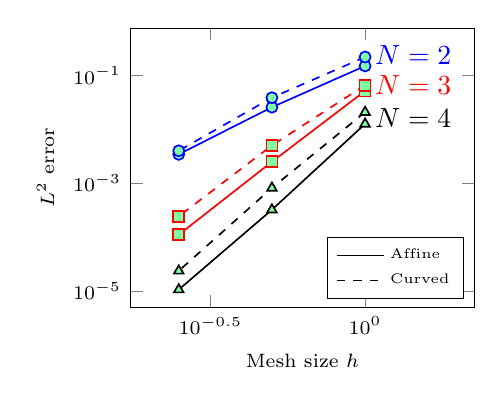
\begin{tikzpicture}
\begin{loglogaxis}[
    legend cell align=left,
    legend style={legend pos=south east, font=\tiny},
    width=.49\textwidth,    
    xlabel={Mesh size $h$},
    ylabel={$L^2$ error}, 
     ymin=5e-6, ymax=.75,    
     xmin=1.75e-1, xmax=2.25,         
    grid style=dashed,
    legend entries={Affine,Curved}
] 
\addlegendimage{no markers,black}
\addlegendimage{no markers,dashed,black}

\addplot[color=blue,mark=*,semithick, mark options={solid,fill=markercolor}]
coordinates{(1,0.149639)(0.5,0.025693)(0.25,0.00342827)} [yshift=4pt] node[right, pos=0, color=blue] {$N = 2$};
\addplot[color=blue,mark=*,dashed,semithick, mark options={solid,fill=markercolor}]
coordinates{(1,0.219501)(0.5,0.0385896)(0.25,0.0039906)};
\logLogSlopeTriangleFlip{0.285}{0.15}{0.6}{3}{blue}


\addplot[color=red,mark=square*,semithick, mark options={solid,fill=markercolor}]
coordinates{(1,0.0516053)(0.5,0.00249425)(0.25,0.000110618)}[yshift=2pt] node[right, pos=0, color=red] {$N = 3$};
\addplot[color=red,mark=square*,dashed,semithick, mark options={solid,fill=markercolor}]
coordinates{(1,0.0657418)(0.5,0.00501536)(0.25,0.000243005)};
\logLogSlopeTriangleFlip{0.285}{0.15}{0.36}{4}{red}

\addplot[color=black,mark=triangle*,semithick, mark options={solid,fill=markercolor}]
coordinates{(1,0.0125714)(0.5,0.000321559)(0.25,1.06097e-05)} [yshift=2pt] node[right, pos=0, color=black] {$N = 4$};
\addplot[color=black,mark=triangle*,dashed,semithick, mark options={solid,fill=markercolor}]
coordinates{(1,0.0207604)(0.5,0.000816006)(0.25,2.36102e-05)};
\logLogSlopeTriangle{0.31}{0.15}{0.05}{5}{black}

%\legend{$L^2$ projection,Weight-adjusted,Difference}
%\legend{Uniform, Optimal, Smoothed}
\end{loglogaxis}
\end{tikzpicture}}
\hspace{.5em}
\subfloat[3D tetrahedral mesh]{
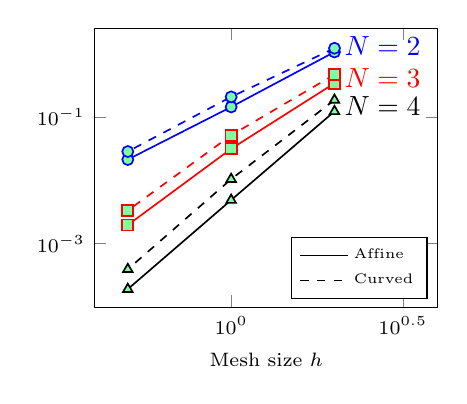
\begin{tikzpicture}
\begin{loglogaxis}[
    legend cell align=left,
    legend style={legend pos=south east, font=\tiny},
    width=.49\textwidth,    
    xlabel={Mesh size $h$},
%    ylabel={$L^2$ error}, 
     ymin=1e-4, ymax=2.5,    
     xmin=4e-1, xmax=4,         
    grid style=dashed,
    legend entries={Affine,Curved}
] 
\addlegendimage{no markers,black}
\addlegendimage{no markers,dashed,black}

\addplot[color=blue,mark=*,semithick, mark options={solid,fill=markercolor}]
coordinates{(2,1.05519)(1,0.143515)(0.5,0.0212682)}[yshift=2pt] node[right, pos=.0, color=blue] {$N = 2$};
\addplot[color=blue,mark=*,dashed,semithick, mark options={solid,fill=markercolor}]
coordinates{(2,1.20915)(1,0.2069)(0.5,0.0284505)};
\logLogSlopeTriangleFlip{0.25}{0.125}{0.6}{3}{blue}

\addplot[color=red,mark=square*,semithick, mark options={solid,fill=markercolor}]
coordinates{(2,0.339318)(1,0.0314342)(0.5,0.00197699)}[yshift=2pt] node[right, pos=0, color=red] {$N = 3$};
\addplot[color=red,mark=square*,dashed,semithick, mark options={solid,fill=markercolor}]
coordinates{(2,0.464613)(1,0.0513369)(0.5,0.00334595)};
\logLogSlopeTriangleFlip{0.25}{0.125}{0.39}{4}{red}

\addplot[color=black,mark=triangle*,semithick, mark options={solid,fill=markercolor}]
coordinates{(2,0.122229)(1,0.00488434)(0.5,0.000192453)}[yshift=2pt] node[right, pos=0, color=black] {$N = 4$};
\addplot[color=black,mark=triangle*,dashed,semithick, mark options={solid,fill=markercolor}]
coordinates{(2,0.184547)(1,0.0104361)(.5,0.0003960681)};
\logLogSlopeTriangle{0.25}{0.125}{0.05}{5}{black}

%\legend{$L^2$ projection,Weight-adjusted,Difference}
%\legend{Uniform, Optimal, Smoothed}
\end{loglogaxis}
\end{tikzpicture}}
\vspace{.33em}
%\caption*{\footnotesize $L^2$ errors for 2D/3D isentropic vortex at $T=5$ on affine, curved meshes.}
\caption*{\footnotesize Accurate numerical integration restores optimal rates of convergence.}
}
\end{figure}
%\only<1>{
%%\vspace{-.25em}
%\begin{itemize}
%%\item Approximation space $P^N$, degree $2N$ volume/face quadratures.
%\item ``Split'' form of derivatives on curved elements for entropy stability.
%%\vspace{.25em}
%\[
%J \pd{u}{x_i} = \frac{1}{2} \sum_{j=1}^d \LRp{J\pd{\hat{x}_j}{x_i} \pd{u}{\hat{x}_j} +  \pd{}{\hat{x}_j}\LRp{J\pd{\hat{x}_j}{x_i}u}}.
%\]
%\item Geometric conservation law (GCL) now \note{necessary} for entropy stability.
%%\vspace{.0025em}
%%\item Generalized ``weight-adjusted'' mass lumping for curved meshes.
%%\item Modify $\tilde{\bm{u}} = \bm{u}\LRp{\tilde{\bm{v}}}$, $\tilde{\bm{v}} = \tilde{P}_N^k\bm{v}(\bm{u}_h)$ using weight-adjusted projection $\tilde{P}^k_N$.
%\end{itemize}
%}

\let\thefootnote\relax\footnotetext{\tiny Visbal and Gaitonde (2002).  On the Use of Higher-Order Finite-Difference Schemes on Curvilinear and Deforming Meshes.}
\let\thefootnote\relax\footnotetext{\tiny Crean, Hicken, et al.\ (2018). \textit{Entropy-stable SBP discretization of the Euler equations on general curved elements.}}
%\let\thefootnote\relax\footnotetext{\tiny Kopriva (2006).  Metric identities and the discontinuous spectral element method on curvilinear meshes.}
%\let\thefootnote\relax\footnotetext{\tiny Chan, Hewett, and Warburton (2016). \textit{Weight-adjusted discontinuous Galerkin methods: curvilinear meshes}.}
%\let\thefootnote\relax\footnotetext{\tiny Chan, Wilcox (2018). \textit{On discretely entropy stable weight-adjusted DG methods: curvilinear meshes}.}
}

%\frame{
%\frametitle{2D curved meshes: conservation of entropy}
%
%\begin{figure}
%\centering
%\subfloat[With weight-adjusted projection]{
%\begin{tikzpicture}
%\begin{semilogyaxis}[
%    legend cell align=left,
%    legend style={legend pos=south east, font=\tiny},
%    width=.48\textwidth,    
%    xlabel={Time $t$},
%    ylabel={Change in entropy $\Delta U(\bm{u})$}, 
%     ymin=1e-9, ymax=5e-4,    
%    grid style=dashed,
%] 
%
%\addplot[color=blue,mark=*,semithick, mark options={solid,fill=markercolor}]
%coordinates{(0.025641,0)(0.128205,1.81455e-05)(0.230769,1.84993e-05)(0.333333,1.81016e-05)(0.435897,2.38212e-05)(0.538462,3.43804e-05)(0.641026,3.75077e-05)(0.74359,3.80509e-05)(0.846154,4.02406e-05)(0.948718,4.57864e-05)(1.05128,5.21023e-05)(1.15385,5.52339e-05)(1.25641,5.93653e-05)(1.35897,6.53204e-05)(1.46154,7.10508e-05)(1.5641,7.58692e-05)(1.66667,8.21148e-05)(1.76923,8.86933e-05)(1.87179,9.52306e-05)(1.97436,0.000102832)};
%%\addplot[color=blue,dashed,semithick, mark options={solid,fill=markercolor}]
%%coordinates{(0.025641,9.95731e-16)(0.128205,4.11303e-15)(0.230769,1.09496e-14)(0.333333,1.86934e-14)(0.435897,1.8624e-14)(0.538462,4.82253e-14)(0.641026,2.80886e-14)(0.74359,3.34073e-14)(0.846154,3.41116e-14)(0.948718,1.12826e-14)(1.05128,1.02106e-14)(1.15385,7.27543e-15)(1.25641,3.21965e-15)(1.35897,2.70617e-15)(1.46154,2.28116e-15)(1.5641,1.01134e-14)(1.66667,9.05179e-15)(1.76923,8.96852e-15)(1.87179,2.69368e-14)(1.97436,1.20043e-15)};
%\addplot[color=red,mark=square*,semithick, mark options={solid,fill=markercolor}]
%coordinates{(0.0129032,0)(0.116129,9.54018e-07)(0.219355,8.64409e-07)(0.322581,7.28292e-07)(0.425806,1.00547e-06)(0.529032,1.54507e-06)(0.632258,1.58376e-06)(0.735484,1.48926e-06)(0.83871,1.52599e-06)(0.941935,1.77263e-06)(1.04516,2.04306e-06)(1.14839,2.10785e-06)(1.25161,2.25231e-06)(1.35484,2.49471e-06)(1.45806,2.7075e-06)(1.56129,2.86391e-06)(1.66452,3.11015e-06)(1.76774,3.35711e-06)(1.87097,3.6045e-06)(1.97419,3.88568e-06)};
%%\addplot[color=red,dotted,semithick, mark options={solid,fill=markercolor}]
%%coordinates{(0.0129032,1.00787e-15)(0.116129,2.48065e-16)(0.219355,8.43769e-15)(0.322581,1.07483e-14)(0.425806,6.18255e-15)(0.529032,4.95159e-14)(0.632258,1.19835e-14)(0.735484,3.68837e-14)(0.83871,2.35957e-14)(0.941935,1.19904e-14)(1.04516,1.73785e-14)(1.14839,7.88952e-15)(1.25161,2.44249e-14)(1.35484,6.38031e-15)(1.45806,1.78781e-14)(1.56129,5.72459e-16)(1.66452,4.02456e-15)(1.76774,1.7316e-14)(1.87097,2.50425e-14)(1.97419,3.55375e-14)};
%\addplot[color=black,mark=pentagon*,semithick, mark options={solid,fill=markercolor}]
%coordinates{(0.00647249,0)(0.110032,5.38994e-08)(0.213592,4.43651e-08)(0.317152,3.18878e-08)(0.420712,4.65967e-08)(0.524272,7.64772e-08)(0.627832,7.36288e-08)(0.731392,6.33475e-08)(0.834951,6.22881e-08)(0.938511,7.43794e-08)(1.04207,8.71374e-08)(1.14563,8.67872e-08)(1.24919,9.19998e-08)(1.35275,1.02781e-07)(1.45631,1.11204e-07)(1.55987,1.16121e-07)(1.66343,1.26634e-07)(1.76699,1.36562e-07)(1.87055,1.46567e-07)(1.97411,1.57581e-07)};
%%\addplot[color=black,dashdotted,semithick, mark options={solid,fill=markercolor}]
%%coordinates{(0.00647249,2.19226e-16)(0.110032,5.88071e-15)(0.213592,1.34059e-14)(0.317152,2.30337e-14)(0.420712,8.23647e-15)(0.524272,2.68709e-14)(0.627832,2.53304e-14)(0.731392,2.95527e-14)(0.834951,2.5948e-14)(0.938511,4.56579e-15)(1.04207,2.28428e-14)(1.14563,8.22259e-15)(1.24919,1.51094e-14)(1.35275,7.86871e-15)(1.45631,1.11508e-14)(1.55987,1.57721e-14)(1.66343,6.95624e-15)(1.76699,2.07681e-14)(1.87055,2.72421e-14)(1.97411,1.7028e-14)};
%
%% % N = 4, K= 8, dt = .25
% % N = 4, K= 8, dt = .125
% % N = 4, K= 8, dt = .0625
%
%%\legend{${\rm CFL} = .25$,${\rm CFL} = .125$,${\rm CFL} = .0625$ }
%%\legend{Uniform, Optimal, Smoothed}
%\end{semilogyaxis}
%\end{tikzpicture}
%}
%\subfloat[Without weight-adjusted projection]{
%\begin{tikzpicture}
%\begin{semilogyaxis}[
%    legend cell align=left,
%    legend style={legend pos=south east, font=\tiny},
%    width=.48\textwidth,
%    xlabel={Time $t$},
%%         ymin=1e-10, ymax=1e-1,    
%%     ymin=1e-7, ymax=1e1,
%     ymin=1e-9, ymax=5e-4,    
%%    ylabel={$L^2$ error}, 
%    grid style=dashed,
%] 
%
%\addplot[color=blue,mark=*,semithick, mark options={solid,fill=markercolor}]
%coordinates{(0.025641,0)(0.128205,4.45681e-05)(0.230769,6.82313e-05)(0.333333,0.000131517)(0.435897,0.000108761)(0.538462,8.51562e-05)(0.641026,2.94791e-05)(0.74359,3.62904e-05)(0.846154,2.97564e-05)(0.948718,9.87886e-05)(1.05128,0.000136806)(1.15385,7.64601e-05)(1.25641,0.000111044)(1.35897,5.72761e-05)(1.46154,4.27e-05)(1.5641,5.03819e-05)(1.66667,4.99789e-05)(1.76923,5.07438e-05)(1.87179,4.26361e-05)(1.97436,2.48694e-05)};
%%\addplot[color=blue,dashed,semithick, mark options={solid,fill=markercolor}]
%%coordinates{(0.025641,5.11743e-16)(0.128205,1.16547e-14)(0.230769,7.91034e-15)(0.333333,1.28231e-14)(0.435897,4.79131e-15)(0.538462,3.44134e-14)(0.641026,6.92502e-15)(0.74359,2.28047e-14)(0.846154,2.15314e-14)(0.948718,4.36456e-15)(1.05128,2.09416e-14)(1.15385,4.86763e-15)(1.25641,3.59088e-15)(1.35897,3.43475e-16)(1.46154,1.03632e-14)(1.5641,1.03598e-14)(1.66667,1.83881e-16)(1.76923,5.94663e-15)(1.87179,3.18252e-14)(1.97436,1.88495e-14)};
%\addplot[color=red,mark=square*,semithick, mark options={solid,fill=markercolor}]
%coordinates{(0.0129032,0)(0.116129,6.48664e-05)(0.219355,8.24474e-05)(0.322581,0.000152373)(0.425806,0.000138342)(0.529032,0.000126709)(0.632258,1.85501e-05)(0.735484,6.98555e-05)(0.83871,7.53129e-05)(0.941935,0.00013915)(1.04516,0.000196476)(1.14839,0.000133645)(1.25161,0.000173751)(1.35484,0.000126668)(1.45806,0.000116008)(1.56129,0.000127919)(1.66452,0.0001343)(1.76774,0.000140992)(1.87097,0.00013971)(1.97419,0.0001291)};
%%\addplot[color=red,dotted,semithick, mark options={solid,fill=markercolor}]
%%coordinates{(0.0129032,3.00107e-16)(0.116129,6.93196e-15)(0.219355,1.00198e-14)(0.322581,7.79932e-15)(0.425806,2.48759e-15)(0.529032,3.46181e-14)(0.632258,1.7205e-14)(0.735484,2.30718e-14)(0.83871,3.0146e-14)(0.941935,9.4369e-15)(1.04516,1.07969e-14)(1.14839,5.59275e-15)(1.25161,5.34295e-15)(1.35484,5.7801e-15)(1.45806,8.74648e-15)(1.56129,1.24137e-14)(1.66452,2.95597e-15)(1.76774,2.64441e-14)(1.87097,2.58023e-14)(1.97419,6.984e-15)};
%\addplot[color=black,mark=pentagon*,semithick, mark options={solid,fill=markercolor}]
%coordinates{(0.00647249,0)(0.110032,6.52844e-05)(0.213592,8.08628e-05)(0.317152,0.000153077)(0.420712,0.000141625)(0.524272,0.000130883)(0.627832,2.58046e-05)(0.731392,6.81127e-05)(0.834951,7.92926e-05)(0.938511,0.000137768)(1.04207,0.000201777)(1.14563,0.000136705)(1.24919,0.000177364)(1.35275,0.000131153)(1.45631,0.000119851)(1.55987,0.000131686)(1.66343,0.000138676)(1.76699,0.00014539)(1.87055,0.000144608)(1.97411,0.000134142)};
%%\addplot[color=black,dashdotted,semithick, mark options={solid,fill=markercolor}]
%%coordinates{(0.00647249,7.31403e-16)(0.110032,1.05055e-14)(0.213592,2.58127e-15)(0.317152,1.04916e-14)(0.420712,5.12437e-15)(0.524272,4.40203e-14)(0.627832,1.147e-14)(0.731392,2.81025e-14)(0.834951,3.01946e-14)(0.938511,4.51028e-15)(1.04207,1.096e-14)(1.14563,6.11317e-15)(1.24919,3.69843e-15)(1.35275,6.47399e-15)(1.45631,9.41608e-15)(1.55987,1.58901e-15)(1.66343,6.39766e-15)(1.76699,1.56819e-14)(1.87055,2.11949e-14)(1.97411,1.12063e-14)};
%
%%\legend{Geo-$(N+1)$, $h^{N+2}$, Geo-$N$, $h^{N+1}$}
%\legend{${\rm CFL} = .25$,${\rm CFL} = .125$,${\rm CFL} = .0625$ }
%\end{semilogyaxis}
%\end{tikzpicture}
%}
%%\subfloat[Convergence of $\Delta S(\bm{u})$]{
%%\begin{tikzpicture}
%%\begin{loglogaxis}[
%%    legend cell align=left,
%%    legend style={legend pos=south east, font=\tiny},
%%    width=.475\textwidth,    
%%    xlabel={Mesh size $h$},
%%    ylabel={$L^2$ error}, 
%%     ymin=5e-6, ymax=2,    
%%     xmin=1e-1, xmax=2.5,         
%%    grid style=dashed,
%%    legend entries={Affine,Curved}
%%] 
%%\addlegendimage{no markers,black}
%%\addlegendimage{no markers,dashed,black}
%%
%%\addplot[color=blue,mark=*,semithick, mark options={solid,fill=markercolor}]
%%coordinates{(2,1.06717)(1,0.149639)(0.5,0.025693)(0.25,0.00342827)} [yshift=4pt] node[left, pos=1.05, color=blue] {$N = 2$};
%%\logLogSlopeTriangleFlip{0.45}{0.15}{0.575}{3}{blue}
%%
%%
%%%\legend{$L^2$ projection,Weight-adjusted,Difference}
%%%\legend{Uniform, Optimal, Smoothed}
%%\end{loglogaxis}
%%\end{tikzpicture}
%%}
%\caption{Change in entropy under an entropy conservative flux with $N=4$.  In both cases, the spatial formulation tested with $\tilde{\bm{v}} = P_N\bm{v}(\bm{u})$ is $O\LRp{10^{-14}}$. }
%%\label{fig:dSconverge}
%\end{figure}
%}

%\frame{
%\frametitle{3D isentropic vortex} 
%\begin{figure}
%\centering
%\subfloat[Affine mesh for $h = 1/2$]{\raisebox{2em}{\includegraphics[width=.425\textwidth]{figs/periodicCube3.png}}\label{subfig:mesh3d}}
%\subfloat[$L^2$ errors]{\begin{tikzpicture}
%\begin{loglogaxis}[
%    legend cell align=left,
%    legend style={legend pos=south east, font=\tiny},
%    width=.55\textwidth,    
%    xlabel={Mesh size $h$},
%    ylabel={$L^2$ error}, 
%     ymin=1e-4, ymax=2,    
%     xmin=4e-1, xmax=4,         
%    grid style=dashed,
%    legend entries={Affine,Curved}
%] 
%\addlegendimage{no markers,black}
%\addlegendimage{no markers,dashed,black}
%
%\addplot[color=blue,mark=*,semithick, mark options={solid,fill=markercolor}]
%coordinates{(2,1.05519)(1,0.143515)(0.5,0.0212682)}[yshift=2pt] node[right, pos=.0, color=blue] {$N = 2$};
%\addplot[color=blue,mark=*,dashed,semithick, mark options={solid,fill=markercolor}]
%coordinates{(2,1.20915)(1,0.2069)(0.5,0.0284505)};
%\logLogSlopeTriangle{0.25}{0.125}{0.525}{3}{blue}
%
%\addplot[color=red,mark=square*,semithick, mark options={solid,fill=markercolor}]
%coordinates{(2,0.339318)(1,0.0314342)(0.5,0.00197699)}[yshift=2pt] node[right, pos=0, color=red] {$N = 3$};
%\addplot[color=red,mark=square*,dashed,semithick, mark options={solid,fill=markercolor}]
%coordinates{(2,0.464613)(1,0.0513369)(0.5,0.00334595)};
%\logLogSlopeTriangle{0.25}{0.125}{0.3}{4}{red}
%
%\addplot[color=black,mark=triangle*,semithick, mark options={solid,fill=markercolor}]
%coordinates{(2,0.122229)(1,0.00488434)(0.5,0.000192453)}[yshift=2pt] node[right, pos=0, color=black] {$N = 4$};
%\addplot[color=black,mark=triangle*,dashed,semithick, mark options={solid,fill=markercolor}]
%coordinates{(2,0.184547)(1,0.0104361)(.5,0.0003960681)};
%\logLogSlopeTriangle{0.25}{0.125}{0.05}{5}{black}
%
%%\legend{$L^2$ projection,Weight-adjusted,Difference}
%%\legend{Uniform, Optimal, Smoothed}
%\end{loglogaxis}
%\end{tikzpicture}}
%\caption{$L^2$ errors at $T=5$ for the 3D isentropic vortex on affine, curved meshes.}
%\label{fig:converge3d}
%\end{figure}
%}

%\frame{
%\frametitle{Inviscid Taylor-Green vortex} 
%%\vspace{-1em}
%\begin{figure}
%\centering
%\includegraphics[width=.65\textwidth]{figs/taylorgreen.png}
%\caption{Isocontours of $z$-vorticity for Taylor-Green at $t = 0, 10$ seconds.}
%\end{figure}
%%\vspace{-.5em}
%\begin{itemize}
%\item Simple turbulence-like behavior (generation of small scales).
%%\vspace{.25em}
%\item Inviscid Taylor-Green: tests robustness w.r.t.\ under-resolved solutions.
%\end{itemize}
%\let\thefootnote\relax\footnotetext{\tiny \url{https://how4.cenaero.be/content/bs1-dns-taylor-green-vortex-re1600}.}
%}
%
%\frame{
%\frametitle{Inviscid Taylor-Green vortex: robust w.r.t.\ under-resolution} 
%%\vspace{-.5em}
%\begin{figure}
%%\centering
%%\only<1>{
%%\subfloat[Kinetic energy ]{
%%\begin{tikzpicture}
%%\begin{axis}[
%%        scaled ticks=false, 
%%        tick label style={/pgf/number format/fixed},
%%	legend cell align=left,
%%	legend style={font=\tiny},
%%	width=.475\textwidth,
%%    xlabel={Time $t$},
%%    ylabel={$\kappa(t)$},
%%%    xmin=.005, xmax=1,
%%%    ymin=1e-10, ymax=1e-1,
%%    legend pos=north east,
%%    xmajorgrids=true,
%%    ymajorgrids=true,
%%    grid style=dashed,
%%%    ytick={0,.001, .005, .01, .015},
%%%    yticklabels={$0$,$\frac{\pi}{2}$,$\pi$,$\frac{3\pi}{2}$},
%%] 
%%\addplot[color=blue,,semithick, mark options={fill=markercolor}]
%%coordinates{(0,0.125)(0.178731,0.125)(0.357462,0.125002)(0.536193,0.125005)(0.714924,0.125009)(0.893655,0.125014)(1.07239,0.125018)(1.25112,0.125023)(1.42985,0.125027)(1.60858,0.125031)(1.78731,0.125034)(1.96604,0.125037)(2.14477,0.125039)(2.3235,0.12504)(2.50223,0.125039)(2.68097,0.125037)(2.8597,0.125032)(3.03843,0.125023)(3.21716,0.125008)(3.39589,0.124984)(3.57462,0.124942)(3.75335,0.124872)(3.93208,0.124756)(4.11081,0.124577)(4.28954,0.124315)(4.46828,0.123948)(4.64701,0.123461)(4.82574,0.122861)(5.00447,0.122182)(5.1832,0.12146)(5.36193,0.120701)(5.54066,0.119905)(5.71939,0.119069)(5.89812,0.118168)(6.07685,0.117182)(6.25558,0.1161)(6.43432,0.1149)(6.61305,0.113564)(6.79178,0.112093)(6.97051,0.110495)(7.14924,0.108768)(7.32797,0.106898)(7.5067,0.104859)(7.68543,0.10263)(7.86416,0.100247)(8.04289,0.0977593)(8.22163,0.0952161)(8.40036,0.092669)(8.57909,0.0901535)(8.75782,0.0876812)(8.93655,0.0852575)(9.11528,0.0828687)(9.29401,0.0804991)(9.47274,0.0781493)(9.65147,0.0758373)(9.83021,0.0735985)(10.0089,0.0714455)(10.1877,0.0693647)(10.3664,0.0673466)(10.5451,0.0653915)(10.7239,0.063496)(10.9026,0.0616565)(11.0813,0.0598745)(11.2601,0.0581523)(11.4388,0.0564894)(11.6175,0.0548814)(11.7962,0.0533217)(11.975,0.0518057)(12.1537,0.0503292)(12.3324,0.0488935)(12.5112,0.0475009)(12.6899,0.0461529)(12.8686,0.0448499)(13.0474,0.0435915)(13.2261,0.0423768)(13.4048,0.0412054)(13.5836,0.0400793)(13.7623,0.0390016)(13.941,0.0379701)(14.1197,0.0369793)(14.2985,0.0360246)(14.4772,0.0351027)(14.6559,0.0342115)(14.8347,0.0333479)(15.0134,0.032511)(15.1921,0.0317027)(15.3709,0.0309235)(15.5496,0.0301727)(15.7283,0.0294487)(15.9071,0.0287493)(16.0858,0.0280732)(16.2645,0.027421)(16.4433,0.0267929)(16.622,0.0261868)(16.8007,0.0256001)(16.9794,0.025031)(17.1582,0.0244798)(17.3369,0.023947)(17.5156,0.0234321)(17.6944,0.0229344)(17.8731,0.0224536)(18.0518,0.0219896)(18.2306,0.0215416)(18.4093,0.0211082)(18.588,0.0206882)(18.7668,0.02028)(18.9455,0.0198829)(19.1242,0.0194966)(19.3029,0.0191212)(19.4817,0.0187558)(19.6604,0.0184)(19.8391,0.0180542)};
%%
%%\addplot[color=red,dashed,semithick, mark options={fill=markercolor}]
%%coordinates{(0,0.125)(0.18796,0.125)(0.37592,0.125002)(0.563879,0.125006)(0.751839,0.125009)(0.939799,0.125014)(1.12776,0.125019)(1.31572,0.125024)(1.50368,0.125028)(1.69164,0.125032)(1.8796,0.125035)(2.06756,0.125037)(2.25552,0.125038)(2.44348,0.125036)(2.63144,0.125032)(2.8194,0.125023)(3.00736,0.125009)(3.19532,0.124985)(3.38328,0.124947)(3.57124,0.124884)(3.7592,0.124781)(3.94716,0.124621)(4.13512,0.124379)(4.32308,0.124027)(4.51104,0.123541)(4.699,0.122909)(4.88696,0.122149)(5.07491,0.121302)(5.26288,0.120396)(5.45083,0.11944)(5.6388,0.118433)(5.82676,0.11736)(6.01471,0.116193)(6.20267,0.114912)(6.39063,0.113497)(6.57859,0.11193)(6.76655,0.110204)(6.95451,0.108334)(7.14247,0.106322)(7.33043,0.104189)(7.51839,0.101934)(7.70635,0.0995426)(7.89431,0.0970654)(8.08227,0.0945369)(8.27023,0.0919787)(8.45819,0.0894304)(8.64615,0.0868905)(8.83411,0.0843671)(9.02207,0.0818692)(9.21003,0.0794052)(9.39799,0.0769825)(9.58595,0.0746288)(9.77391,0.0723431)(9.96187,0.0701295)(10.1498,0.0679956)(10.3378,0.0659364)(10.5258,0.0639473)(10.7137,0.0620322)(10.9017,0.0601792)(11.0896,0.0583829)(11.2776,0.0566368)(11.4656,0.0549345)(11.6535,0.053277)(11.8415,0.0516697)(12.0294,0.0501198)(12.2174,0.0486301)(12.4053,0.047197)(12.5933,0.0458163)(12.7813,0.0444834)(12.9692,0.0431979)(13.1572,0.0419597)(13.3451,0.0407697)(13.5331,0.0396274)(13.7211,0.038527)(13.909,0.0374678)(14.097,0.0364487)(14.2849,0.0354663)(14.4729,0.034518)(14.6609,0.0336038)(14.8488,0.0327232)(15.0368,0.0318737)(15.2247,0.0310535)(15.4127,0.0302625)(15.6007,0.0295011)(15.7886,0.0287685)(15.9766,0.0280626)(16.1645,0.0273818)(16.3525,0.0267242)(16.5405,0.0260884)(16.7284,0.0254745)(16.9164,0.0248826)(17.1043,0.0243113)(17.2923,0.0237595)(17.4803,0.0232271)(17.6682,0.0227134)(17.8562,0.0222159)(18.0441,0.0217324)(18.2321,0.0212626)(18.4201,0.0208084)(18.608,0.0203709)(18.796,0.019949)(18.9839,0.0195411)(19.1719,0.0191457)(19.3599,0.0187618)(19.5478,0.0183882)(19.7358,0.0180246)(19.9237,0.0176713)};
%%
%%\legend{Affine, Curved}
%%\end{axis}\end{tikzpicture}
%%}
%%\hspace{.25em}
%%\subfloat[KE dissipation rate]{% ($N=3$, $h = {\pi}/ {8}$)]{
%%\begin{tikzpicture}
%%\begin{axis}[
%%        scaled ticks=false, 
%%        tick label style={/pgf/number format/fixed},
%%	legend cell align=left,
%%	legend style={font=\tiny},
%%	width=.475\textwidth,
%%    xlabel={Time $t$},
%%    ylabel={$-\pd{\kappa}{t}$},
%%%    xmin=.005, xmax=1,
%%%    ymin=1e-10, ymax=1e-1,
%%ymin=-.0025, ymax=.017,
%%    legend pos=north east,
%%    xmajorgrids=true,
%%    ymajorgrids=true,
%%    grid style=dashed,
%%    ytick={0, .005, .01, .015},
%%    yticklabels={0, .005, .01, .015}    
%%] 
%%\addplot[color=blue,semithick, mark options={fill=markercolor}]
%%coordinates{(0.007149,-0)(0.207328,-1.12783e-05)(0.407507,-1.46618e-05)(0.607685,-2.53763e-05)(0.807864,-2.98876e-05)(1.00804,-2.65041e-05)(1.20822,-3.15793e-05)(1.4084,-2.48123e-05)(1.60858,-1.97371e-05)(1.80876,-2.42484e-05)(2.00894,-2.0301e-05)(2.20912,-1.40979e-05)(2.40929,-6.767e-06)(2.60947,1.12783e-05)(2.80965,2.98876e-05)(3.00983,6.31587e-05)(3.21001,0.000110528)(3.41019,0.000181581)(3.61037,0.000329891)(3.81054,0.00058027)(4.01072,0.000940613)(4.2109,0.00144081)(4.41108,0.00207803)(4.61126,0.00279816)(4.81144,0.00343031)(5.01162,0.00381377)(5.2118,0.00407881)(5.41197,0.00431791)(5.61215,0.00455532)(5.81233,0.00493822)(6.01251,0.00546492)(6.21269,0.00609087)(6.41287,0.00687415)(6.61305,0.00773299)(6.81323,0.00853827)(7.0134,0.00933057)(7.21358,0.010159)(7.41376,0.0111904)(7.61394,0.0123673)(7.81412,0.0132419)(8.0143,0.013865)(8.21448,0.0140928)(8.41466,0.0139739)(8.61483,0.0137714)(8.81501,0.0135272)(9.01519,0.0133541)(9.21537,0.0133011)(9.41555,0.0131477)(9.61573,0.0127451)(9.81591,0.012215)(10.0161,0.0117295)(10.2163,0.0113731)(10.4164,0.0110065)(10.6166,0.0106795)(10.8168,0.0103857)(11.017,0.0100281)(11.2172,0.00961873)(11.4173,0.00931591)(11.6175,0.00903677)(11.8177,0.0087441)(12.0179,0.00844409)(12.2181,0.00816101)(12.4182,0.0078689)(12.6184,0.00757115)(12.8186,0.00726438)(13.0188,0.00696776)(13.2189,0.00667621)(13.4191,0.00640158)(13.6193,0.00614162)(13.8195,0.0058918)(14.0197,0.00565214)(14.2198,0.00541755)(14.42,0.00519085)(14.6202,0.0049839)(14.8204,0.00477863)(15.0206,0.0045728)(15.2207,0.00437148)(15.4209,0.00419272)(15.6211,0.00402693)(15.8213,0.00386339)(16.0214,0.00371678)(16.2216,0.00359948)(16.4218,0.00349347)(16.622,0.00337222)(16.8222,0.00324083)(17.0223,0.00311451)(17.2225,0.00299835)(17.4227,0.00289571)(17.6229,0.00280323)(17.8231,0.00270906)(18.0232,0.00261432)(18.2234,0.00252071)(18.4236,0.00243612)(18.6238,0.00235717)(18.8239,0.00227371)(19.0241,0.00218913)(19.2243,0.00211187)(19.4245,0.00204025)(19.6247,0.00197089)(19.8248,0.00190548)};
%%
%%\addplot[color=red, dashed,semithick, mark options={fill=markercolor}]
%%coordinates{(0.00662,-0)(0.20523,-1.01505e-05)(0.40384,-1.24062e-05)(0.60245,-2.31206e-05)(0.801059,-2.59402e-05)(0.999669,-2.31206e-05)(1.19828,-2.81958e-05)(1.39689,-2.19928e-05)(1.5955,-1.80453e-05)(1.79411,-2.14288e-05)(1.99272,-1.86093e-05)(2.19133,-1.63536e-05)(2.38994,-8.45875e-06)(2.58855,5.07525e-06)(2.78716,2.0301e-05)(2.98577,4.96247e-05)(3.18438,9.4738e-05)(3.38299,0.000160152)(3.5816,0.000283086)(3.78021,0.000504706)(3.97881,0.000825574)(4.17743,0.00126543)(4.37603,0.00183499)(4.57464,0.00247672)(4.77325,0.0030897)(4.97186,0.00349741)(5.17047,0.00375061)(5.36908,0.00398971)(5.56769,0.00419893)(5.7663,0.00449555)(5.96491,0.00496811)(6.16352,0.00551849)(6.36213,0.00618335)(6.56074,0.00695535)(6.75935,0.00776796)(6.95796,0.00847567)(7.15657,0.00922568)(7.35518,0.0102655)(7.55379,0.0113212)(7.7524,0.0122049)(7.95101,0.0127772)(8.14962,0.0130801)(8.34823,0.0132329)(8.54684,0.0131302)(8.74545,0.012815)(8.94406,0.0124564)(9.14267,0.0121327)(9.34128,0.0117836)(9.53989,0.0115276)(9.7385,0.0112761)(9.93711,0.0109236)(10.1357,0.0105819)(10.3343,0.0102689)(10.5329,0.0100225)(10.7315,0.00976309)(10.9302,0.00945689)(11.1288,0.00915857)(11.3274,0.00887436)(11.526,0.00861327)(11.7246,0.00831947)(11.9232,0.00802623)(12.1218,0.00775273)(12.3204,0.00746513)(12.519,0.00717584)(12.7176,0.00690742)(12.9163,0.00662038)(13.1149,0.00633448)(13.3135,0.00608184)(13.5121,0.00583767)(13.7107,0.00559631)(13.9093,0.00538653)(14.1079,0.00517958)(14.3065,0.00497093)(14.5051,0.00477976)(14.7037,0.00457393)(14.9024,0.00436246)(15.101,0.00417242)(15.2996,0.00400832)(15.4982,0.00385719)(15.6968,0.00370663)(15.8954,0.00355042)(16.094,0.00340831)(16.2926,0.00329102)(16.4912,0.00318557)(16.6898,0.00307729)(16.8884,0.00296056)(17.0871,0.00284214)(17.2857,0.00272597)(17.4843,0.00261714)(17.6829,0.00252353)(17.8815,0.00243725)(18.0801,0.00234984)(18.2787,0.00226413)(18.4773,0.00218349)(18.6759,0.0021051)(18.8745,0.00202954)(19.0732,0.00195848)(19.2718,0.00189589)(19.4704,0.00184288)(19.669,0.00179438)(19.8676,0.00174476)};
%%
%%\legend{Affine, Curved}
%%\end{axis}\end{tikzpicture}
%%}
%%}
%\only<1>{
%%\subfloat[KE dissipation rate from Gassner, Winters, Kopriva (2016) ]{
%%\includegraphics[width=.4\textwidth]{figs/gassner_dkedt.png}
%%}
%%\hspace{.25em}
%%\subfloat[KE dissipation rate]{
%\begin{tikzpicture}
%\begin{axis}[
%        scaled ticks=false, 
%        tick label style={/pgf/number format/fixed},
%    legend pos=north east, 
%    	legend cell align=left,
%	legend style={font=\tiny},        
%	width=.68\textwidth,
%    xlabel={Time $t$},
%    ylabel={$-\pd{\kappa}{t}$},
%    xmin=0, xmax=20,
%ymin=-.0025, ymax=.016,
%    xmajorgrids=true,
%    ymajorgrids=true,
%    grid style=dashed,
%    ytick={-.002,  .002, .006,.01, .014},
%    yticklabels={-.002,  .002, .006,.01,   .014}    
%] 
%\addplot[color=blue,semithick, mark options={fill=markercolor}]
%coordinates{(0.007149,-0)(0.207328,-1.12783e-05)(0.407507,-1.46618e-05)(0.607685,-2.53763e-05)(0.807864,-2.98876e-05)(1.00804,-2.65041e-05)(1.20822,-3.15793e-05)(1.4084,-2.48123e-05)(1.60858,-1.97371e-05)(1.80876,-2.42484e-05)(2.00894,-2.0301e-05)(2.20912,-1.40979e-05)(2.40929,-6.767e-06)(2.60947,1.12783e-05)(2.80965,2.98876e-05)(3.00983,6.31587e-05)(3.21001,0.000110528)(3.41019,0.000181581)(3.61037,0.000329891)(3.81054,0.00058027)(4.01072,0.000940613)(4.2109,0.00144081)(4.41108,0.00207803)(4.61126,0.00279816)(4.81144,0.00343031)(5.01162,0.00381377)(5.2118,0.00407881)(5.41197,0.00431791)(5.61215,0.00455532)(5.81233,0.00493822)(6.01251,0.00546492)(6.21269,0.00609087)(6.41287,0.00687415)(6.61305,0.00773299)(6.81323,0.00853827)(7.0134,0.00933057)(7.21358,0.010159)(7.41376,0.0111904)(7.61394,0.0123673)(7.81412,0.0132419)(8.0143,0.013865)(8.21448,0.0140928)(8.41466,0.0139739)(8.61483,0.0137714)(8.81501,0.0135272)(9.01519,0.0133541)(9.21537,0.0133011)(9.41555,0.0131477)(9.61573,0.0127451)(9.81591,0.012215)(10.0161,0.0117295)(10.2163,0.0113731)(10.4164,0.0110065)(10.6166,0.0106795)(10.8168,0.0103857)(11.017,0.0100281)(11.2172,0.00961873)(11.4173,0.00931591)(11.6175,0.00903677)(11.8177,0.0087441)(12.0179,0.00844409)(12.2181,0.00816101)(12.4182,0.0078689)(12.6184,0.00757115)(12.8186,0.00726438)(13.0188,0.00696776)(13.2189,0.00667621)(13.4191,0.00640158)(13.6193,0.00614162)(13.8195,0.0058918)(14.0197,0.00565214)(14.2198,0.00541755)(14.42,0.00519085)(14.6202,0.0049839)(14.8204,0.00477863)(15.0206,0.0045728)(15.2207,0.00437148)(15.4209,0.00419272)(15.6211,0.00402693)(15.8213,0.00386339)(16.0214,0.00371678)(16.2216,0.00359948)(16.4218,0.00349347)(16.622,0.00337222)(16.8222,0.00324083)(17.0223,0.00311451)(17.2225,0.00299835)(17.4227,0.00289571)(17.6229,0.00280323)(17.8231,0.00270906)(18.0232,0.00261432)(18.2234,0.00252071)(18.4236,0.00243612)(18.6238,0.00235717)(18.8239,0.00227371)(19.0241,0.00218913)(19.2243,0.00211187)(19.4245,0.00204025)(19.6247,0.00197089)(19.8248,0.00190548)};
%
%\addplot[color=red, dashed,semithick, mark options={fill=markercolor}]
%coordinates{(0.00662,-0)(0.20523,-1.01505e-05)(0.40384,-1.24062e-05)(0.60245,-2.31206e-05)(0.801059,-2.59402e-05)(0.999669,-2.31206e-05)(1.19828,-2.81958e-05)(1.39689,-2.19928e-05)(1.5955,-1.80453e-05)(1.79411,-2.14288e-05)(1.99272,-1.86093e-05)(2.19133,-1.63536e-05)(2.38994,-8.45875e-06)(2.58855,5.07525e-06)(2.78716,2.0301e-05)(2.98577,4.96247e-05)(3.18438,9.4738e-05)(3.38299,0.000160152)(3.5816,0.000283086)(3.78021,0.000504706)(3.97881,0.000825574)(4.17743,0.00126543)(4.37603,0.00183499)(4.57464,0.00247672)(4.77325,0.0030897)(4.97186,0.00349741)(5.17047,0.00375061)(5.36908,0.00398971)(5.56769,0.00419893)(5.7663,0.00449555)(5.96491,0.00496811)(6.16352,0.00551849)(6.36213,0.00618335)(6.56074,0.00695535)(6.75935,0.00776796)(6.95796,0.00847567)(7.15657,0.00922568)(7.35518,0.0102655)(7.55379,0.0113212)(7.7524,0.0122049)(7.95101,0.0127772)(8.14962,0.0130801)(8.34823,0.0132329)(8.54684,0.0131302)(8.74545,0.012815)(8.94406,0.0124564)(9.14267,0.0121327)(9.34128,0.0117836)(9.53989,0.0115276)(9.7385,0.0112761)(9.93711,0.0109236)(10.1357,0.0105819)(10.3343,0.0102689)(10.5329,0.0100225)(10.7315,0.00976309)(10.9302,0.00945689)(11.1288,0.00915857)(11.3274,0.00887436)(11.526,0.00861327)(11.7246,0.00831947)(11.9232,0.00802623)(12.1218,0.00775273)(12.3204,0.00746513)(12.519,0.00717584)(12.7176,0.00690742)(12.9163,0.00662038)(13.1149,0.00633448)(13.3135,0.00608184)(13.5121,0.00583767)(13.7107,0.00559631)(13.9093,0.00538653)(14.1079,0.00517958)(14.3065,0.00497093)(14.5051,0.00477976)(14.7037,0.00457393)(14.9024,0.00436246)(15.101,0.00417242)(15.2996,0.00400832)(15.4982,0.00385719)(15.6968,0.00370663)(15.8954,0.00355042)(16.094,0.00340831)(16.2926,0.00329102)(16.4912,0.00318557)(16.6898,0.00307729)(16.8884,0.00296056)(17.0871,0.00284214)(17.2857,0.00272597)(17.4843,0.00261714)(17.6829,0.00252353)(17.8815,0.00243725)(18.0801,0.00234984)(18.2787,0.00226413)(18.4773,0.00218349)(18.6759,0.0021051)(18.8745,0.00202954)(19.0732,0.00195848)(19.2718,0.00189589)(19.4704,0.00184288)(19.669,0.00179438)(19.8676,0.00174476)};
%
%\addplot[smooth,color=black,dashdotted,semithick, mark options={solid,fill=markercolor}]
%  coordinates{(0.0,0) (0.28719,0) (0.53378,0) (0.78906,0) (1.04434,0) (1.29963,0) (1.54041,0) (1.80439,0) (2.05097,6.28e-06) (2.29755,2.197e-05) (2.54994,2.51e-05) (2.79942,2.51e-05) (3.0518,5.334e-05) (3.30709,7.845e-05) (3.54206,0.00019141) (3.80025,0.00042989) (4.04112,0.00079443) (4.28761,0.00123005) (4.53129,0.00216199) (4.76046,0.00295274) (5.00705,0.0031567) (5.25073,0.00304373) (5.4857,0.00352069) (5.73518,0.0045405) (5.75839,0.00465815) (5.82703,0.0048383) (5.90054,0.00495156) (5.97306,0.00503628) (6.03978,0.00505511) (6.08399,0.0051618) (6.20804,0.00570151) (6.43722,0.00715434) (6.7041,0.0078635) (6.82884,0.00798902) (6.91587,0.00831222) (7.04932,0.00895862) (7.18856,0.00906844) (7.25238,0.00924417) (7.2988,0.00955481) (7.33941,0.00986546) (7.40033,0.01016356) (7.57149,0.01044911) (7.73394,0.01032987) (7.83838,0.01067503) (7.88479,0.01098255) (7.93701,0.01129633) (7.98632,0.01160384) (8.10816,0.01222828) (8.33444,0.01312257) (8.42884,0.01330112) (8.46259,0.0131414) (8.49792,0.0129375) (8.61293,0.01200549) (8.68835,0.01169798) (8.70286,0.01164464) (8.8305,0.01179212) (9.01027,0.01269896) (9.1776,0.01250441) (9.28595,0.01280565) (9.32366,0.01310688) (9.37298,0.01343008) (9.40199,0.0137376) (9.46291,0.01401373) (9.49482,0.01383173) (9.54414,0.01352108) (9.59055,0.0130504) (9.65727,0.0124291) (9.7385,0.01182663) (9.92706,0.01139674) (9.99668,0.01108296) (10.08661,0.01059345) (10.20845,0.01000981) (10.23746,0.00986233) (10.3448,0.00955795) (10.43763,0.00946695) (10.50435,0.0093132) (10.67261,0.00888017) (10.73063,0.00874211) (10.88438,0.00856952) (11.02362,0.00886135) (11.11935,0.00918141) (11.2528,0.0094293) (11.37754,0.00914689) (11.45006,0.00885507) (11.52549,0.00853501) (11.62122,0.00824946) (11.73436,0.00795136) (11.84169,0.00787919) (12.00995,0.0078384) (12.11148,0.00757796) (12.21881,0.00729555) (12.30004,0.00698804) (12.38417,0.00668994) (12.45379,0.00638243) (12.54372,0.00609688) (12.72068,0.00583644) (12.97596,0.00583016) (13.20514,0.00605609) (13.2963,0.0061533) (13.42754,0.00631269) (13.54745,0.00619729) (13.64608,0.00590233) (13.73021,0.00559796) (13.84045,0.00530928) (13.97389,0.00503314) (13.9913,0.00499504)};
%
% 
%\legend{Affine, Curved, Gassner et al.}% , Beck et al.\ (viscous), Spectral (viscous)}
%\end{axis}\end{tikzpicture}
%%}
%}
%%\caption{Evolution of kinetic energy $\kappa(t)$ and kinetic energy dissipation rate $-\pd{\kappa}{t}$ for $N=3, h = \pi/8, \text{CFL} = .25$ on affine and curved meshes.}
%\caption*{Kinetic energy dissipation rate $-\pd{\kappa}{t}$ for $N=3, h = \pi/8, \text{CFL} = .25$ (tet meshes).}% on affine and curved meshes.}
%\end{figure}
%}


\subsection{Quad and hex meshes: new collocation schemes}

\frame[noframenumbering]{
\frametitle{Talk outline}
\tableofcontents[currentsection,currentsubsection]
}


\frame{
\frametitle{Entropy stable Gauss collocation on tensor product elements (with MH Carpenter + DCDR Fernandez)}
\begin{columns}
\hspace{-.5em}
\begin{column}{.49\textwidth}
\vspace{-.5em}
\begin{figure}
\centering
\begin{overlayarea}{.75\textwidth}{.425\textheight}
\only<1>{\includegraphics[height=.425\textheight]{figs/gsbp1.png}}
\only<2>{\includegraphics[height=.425\textheight]{figs/gsbp2.png}}
\only<3>{\includegraphics[height=.425\textheight]{figs/gsbp3.png}}
\only<4>{\includegraphics[height=.425\textheight]{figs/gsbp4.png}}
%\includegraphics[height=.45\textheight]{figs/gsbp4.png}
\end{overlayarea}
\end{figure}
\end{column}
%\vspace{-2.5em}
\hspace{3em}
\begin{column}{.51\textwidth}
\[
\only<1>{
\LRp{\underbrace{\begin{bmatrix}
\bm{A} & \bm{B}\\
-\bm{B}^T & \bm{C}
\end{bmatrix}}_{\bm{Q}_h^i} \circ
\underbrace{\begin{bmatrix}
\bm{F}_{vv} & \bm{F}_{vf}\\
\bm{F}_{fv} & \bm{F}_{ff}
\end{bmatrix}}_{\bm{F}} } \bm{1}
}
\only<2>{
\LRp{\underbrace{\begin{bmatrix}
\note{\bm{A}} & \bm{B}\\
-\bm{B}^T & \bm{C}
\end{bmatrix}}_{\bm{Q}_h^i} \circ
\underbrace{\begin{bmatrix}
\note{\bm{F}_{vv}} & \bm{F}_{vf}\\
\bm{F}_{fv} & \bm{F}_{ff}
\end{bmatrix}}_{\bm{F}} } \bm{1}
}
\only<3>{
\LRp{\underbrace{\begin{bmatrix}
\bm{A} & \bm{B}\\
-\bm{B}^T & \note{\bm{C}}
\end{bmatrix}}_{\bm{Q}_h^i} \circ
\underbrace{\begin{bmatrix}
\bm{F}_{vv} & \bm{F}_{vf}\\
\bm{F}_{fv} & \note{\bm{F}_{ff}}
\end{bmatrix}}_{\bm{F}} } \bm{1}
}
\only<4>{
\LRp{\underbrace{\begin{bmatrix}
\bm{A} & \note{\bm{B}}\\
\note{-\bm{B}^T} & \bm{C}
\end{bmatrix}}_{\bm{Q}_h^i} \circ
\underbrace{\begin{bmatrix}
\bm{F}_{vv} & \note{\bm{F}_{vf}}\\
\note{\bm{F}_{fv}} & \bm{F}_{ff}
\end{bmatrix}}_{\bm{F}} } \bm{1}
}
\]
\end{column}
\end{columns}
\vspace{.5em}
\begin{itemize}
\item Hexahedral elements: tensor product polynomial basis
\vspace{.5em}
\item Tensor product $(N+1)$-point Gauss quadrature for integrals.
\vspace{.5em}
\item Advantage of hexes vs.\ tets: simplifies to \note{collocation}, Kronecker product reduces flux evaluations from $O(N^6)$ to $O(N^4)$ in 3D.
\vspace{.5em}
\end{itemize} 
}


\frame{
\frametitle{Gauss quadrature improves errors on warped meshes}

\begin{figure}
\centering
\begin{overlayarea}{\textwidth}{.55\textheight}
\only<1>{
\raisebox{3.5em}{\includegraphics[width=.475\textwidth]{figs/warp2d_a0.png}}
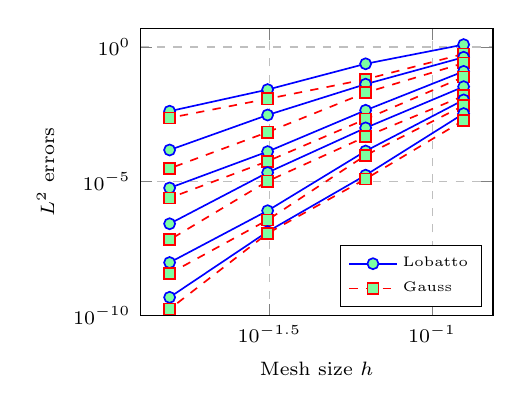
\begin{tikzpicture}
\begin{loglogaxis}[
    width=.5\textwidth,
    xlabel={Mesh size $h$},
    ylabel={$L^2$ errors}, 
%    xmin=.0125, 
    ymin=1e-10, ymax=5,
    legend pos=south east, legend cell align=left, legend style={font=\tiny},	
    xmajorgrids=true, ymajorgrids=true, grid style=dashed,
    legend entries={Lobatto, Gauss}    
]
\pgfplotsset{
cycle list={{blue, mark=*}, {red, dashed ,mark=square*}}
}
\addplot+[semithick, mark options={solid, fill=markercolor}]
coordinates{(0.125,1.22861)(0.0625,0.236646)(0.03125,0.0258883)(0.015625,0.00406122)};
\addplot+[semithick, mark options={solid, fill=markercolor}]
coordinates{(0.125,0.553435)(0.0625,0.0625441)(0.03125,0.0117156)(0.015625,0.0022841)}; %(0.0078125,0.000362526)

\addplot+[semithick, mark options={solid, fill=markercolor}]
coordinates{(0.125,0.414449)(0.0625,0.0412224)(0.03125,0.00293039)(0.015625,0.000145701)};
\addplot+[semithick, mark options={solid, fill=markercolor}]
coordinates{(0.125,0.25082)(0.0625,0.0198863)(0.03125,0.000673152)(0.015625,2.98263e-05)}; %(0.0078125, 1.77421e-06)

\addplot+[semithick, mark options={solid, fill=markercolor}]
coordinates{(0.125,0.123516)(0.0625,0.00439285)(0.03125,0.000126852)(0.015625,5.61786e-06)};
\addplot+[semithick, mark options={solid, fill=markercolor}]
coordinates{(0.125,0.0768018)(0.0625,0.0020579)(0.03125,5.55322e-05)(0.015625,2.36108e-06)}; % (0.0078125,8.55848e-08)

\addplot+[semithick, mark options={solid, fill=markercolor}]
coordinates{(0.125,0.0332509)(0.0625,0.000970148)(0.03125,2.10334e-05)(0.015625,2.60008e-07)};
\addplot+[semithick, mark options={solid, fill=markercolor}]
coordinates{(0.125,0.0151231)(0.0625,0.000454595)(0.03125,1.00203e-05)(0.015625,6.57796e-08)}; %(0.0078125, 9.32809e-10)

\addplot+[semithick, mark options={solid, fill=markercolor}]
coordinates{(0.125,0.0106752)(0.0625,0.000133284)(0.03125,7.97032e-07)(0.015625,9.35152e-09)};
\addplot+[semithick, mark options={solid, fill=markercolor}]
coordinates{(0.125,0.00657096)(0.0625,9.22845e-05)(0.03125,3.60025e-07)(0.015625,3.63974e-09)}; %(0.0078125, 1.23726e-10)

\addplot+[semithick, mark options={solid, fill=markercolor}]
coordinates{(0.125,0.00330917)(0.0625,1.67825e-05)(0.03125,1.32696e-07)(0.015625,4.73518e-10)};
\addplot+[semithick, mark options={solid, fill=markercolor}]
coordinates{(0.125,0.00185273)(0.0625,1.21465e-05)(0.03125,1.14289e-07)(0.015625,1.72358e-10)}; 

\end{loglogaxis}
\end{tikzpicture}
}
\only<2>{
\raisebox{3.5em}{\includegraphics[width=.475\textwidth]{figs/warp2d_a0312.png}}
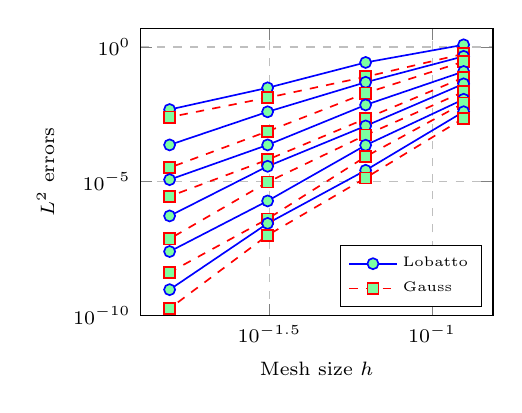
\begin{tikzpicture}
\begin{loglogaxis}[
    width=.5\textwidth,
    xlabel={Mesh size $h$},
    ylabel={$L^2$ errors}, 
%    xmin=.0125, 
    ymin=1e-10, ymax=5,
    legend pos=south east, legend cell align=left, legend style={font=\tiny},	
    xmajorgrids=true, ymajorgrids=true, grid style=dashed,
    legend entries={Lobatto, Gauss}    
]
\pgfplotsset{
cycle list={{blue, mark=*}, {red, dashed ,mark=square*}}
}
\addplot+[semithick, mark options={solid, fill=markercolor}]
coordinates{(0.125,1.2082)(0.0625,0.265357)(0.03125,0.0301118)(0.015625,0.00467693)};
\addplot+[semithick, mark options={solid, fill=markercolor}]
coordinates{(0.125,0.555586)(0.0625,0.0773534)(0.03125,0.0129171)(0.015625,0.0024363)};
\addplot+[semithick, mark options={solid, fill=markercolor}]
coordinates{(0.125,0.448878)(0.0625,0.0485323)(0.03125,0.00385418)(0.015625,0.000225396)};
\addplot+[semithick, mark options={solid, fill=markercolor}]
coordinates{(0.125,0.287685)(0.0625,0.0190431)(0.03125,0.000721055)(0.015625,3.19095e-05)};
\addplot+[semithick, mark options={solid, fill=markercolor}]
coordinates{(0.125,0.122081)(0.0625,0.00694351)(0.03125,0.000224524)(0.015625,1.14555e-05)};
\addplot+[semithick, mark options={solid, fill=markercolor}]
coordinates{(0.125,0.0731583)(0.0625,0.00213914)(0.03125,6.32128e-05)(0.015625,2.73037e-06)};
\addplot+[semithick, mark options={solid, fill=markercolor}]
coordinates{(0.125,0.0424351)(0.0625,0.00114569)(0.03125,3.59697e-05)(0.015625,5.09643e-07)};
\addplot+[semithick, mark options={solid, fill=markercolor}]
coordinates{(0.125,0.0215298)(0.0625,0.000523714)(0.03125,9.27521e-06)(0.015625,7.14031e-08)};
\addplot+[semithick, mark options={solid, fill=markercolor}]
coordinates{(0.125,0.0112838)(0.0625,0.000219049)(0.03125,1.84304e-06)(0.015625,2.40402e-08)};
\addplot+[semithick, mark options={solid, fill=markercolor}]
coordinates{(0.125,0.00809138)(0.0625,8.23415e-05)(0.03125,3.95565e-07)(0.015625,4.01268e-09)};
\addplot+[semithick, mark options={solid, fill=markercolor}]
coordinates{(0.125,0.00388316)(0.0625,2.55074e-05)(0.03125,2.68102e-07)(0.015625,9.13754e-10)};
\addplot+[semithick, mark options={solid, fill=markercolor}]
coordinates{(0.125,0.00222029)(0.0625,1.33111e-05)(0.03125,9.72405e-08)(0.015625,1.81386e-10)};

\end{loglogaxis}
\end{tikzpicture}
}
\only<3>{
\raisebox{3.5em}{\includegraphics[width=.475\textwidth]{figs/warp2d_a125.png}}
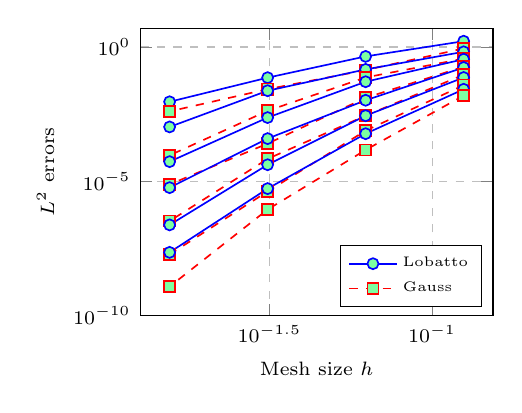
\begin{tikzpicture}
\begin{loglogaxis}[
    width=.5\textwidth,
    xlabel={Mesh size $h$},
    ylabel={$L^2$ errors}, 
%    xmin=.0125,
    ymin=1e-10, ymax=5,
    legend pos=south east, legend cell align=left, legend style={font=\tiny},	
    xmajorgrids=true, ymajorgrids=true, grid style=dashed,
    legend entries={Lobatto, Gauss}    
]
\pgfplotsset{
cycle list={{blue, mark=*}, {red, dashed ,mark=square*}}
}
\addplot+[semithick, mark options={solid, fill=markercolor}]
coordinates{(0.125,1.64274)(0.0625,0.445945)(0.03125,0.0720148)(0.015625,0.0091066)};
\addplot+[semithick, mark options={solid, fill=markercolor}]
coordinates{(0.125,0.882247)(0.0625,0.138116)(0.03125,0.0268145)(0.015625,0.0039945)};
\addplot+[semithick, mark options={solid, fill=markercolor}]
coordinates{(0.125,0.662165)(0.0625,0.146131)(0.03125,0.0234934)(0.015625,0.00105368)};
\addplot+[semithick, mark options={solid, fill=markercolor}]
coordinates{(0.125,0.368084)(0.0625,0.0734059)(0.03125,0.00420438)(0.015625,9.19378e-05)};
\addplot+[semithick, mark options={solid, fill=markercolor}]
coordinates{(0.125,0.349184)(0.0625,0.0508268)(0.03125,0.00234785)(0.015625,5.36192e-05)};
\addplot+[semithick, mark options={solid, fill=markercolor}]
coordinates{(0.125,0.183472)(0.0625,0.0127617)(0.03125,0.000251929)(0.015625,7.6013e-06)};
\addplot+[semithick, mark options={solid, fill=markercolor}]
coordinates{(0.125,0.171986)(0.0625,0.0103578)(0.03125,0.000386834)(0.015625,5.76284e-06)};
\addplot+[semithick, mark options={solid, fill=markercolor}]
coordinates{(0.125,0.0924215)(0.0625,0.00276519)(0.03125,6.80528e-05)(0.015625,3.27246e-07)};
\addplot+[semithick, mark options={solid, fill=markercolor}]
coordinates{(0.125,0.0729963)(0.0625,0.00276104)(0.03125,4.11305e-05)(0.015625,2.36125e-07)};
\addplot+[semithick, mark options={solid, fill=markercolor}]
coordinates{(0.125,0.0378013)(0.0625,0.0007649)(0.03125,4.15848e-06)(0.015625,1.8685e-08)};
\addplot+[semithick, mark options={solid, fill=markercolor}]
coordinates{(0.125,0.026577)(0.0625,0.000589552)(0.03125,5.3039e-06)(0.015625,2.23719e-08)};
\addplot+[semithick, mark options={solid, fill=markercolor}]
coordinates{(0.125,0.0154563)(0.0625,0.000146207)(0.03125,8.83156e-07)(0.015625,1.18829e-09)};

\end{loglogaxis}
\end{tikzpicture}
}
\only<4>{
\raisebox{3.5em}{\includegraphics[width=.475\textwidth]{figs/warp2d_a25.png}}
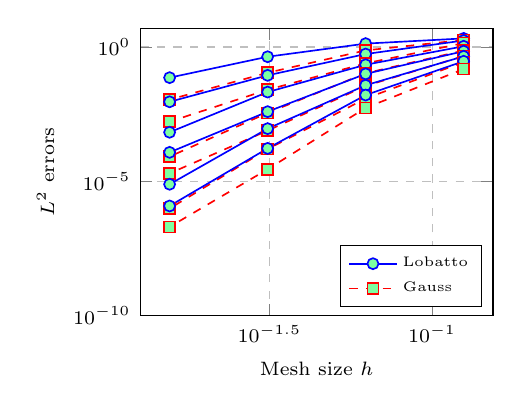
\begin{tikzpicture}
\begin{loglogaxis}[
    width=.5\textwidth,
    xlabel={Mesh size $h$},
    ylabel={$L^2$ errors}, 
%    xmin=.0125,
    ymin=1e-10, ymax=5,
    legend pos=south east, legend cell align=left, legend style={font=\tiny},	
    xmajorgrids=true, ymajorgrids=true, grid style=dashed,
    legend entries={Lobatto, Gauss}    
]
\pgfplotsset{
cycle list={{blue, mark=*}, {red, dashed ,mark=square*}}
}
\addplot+[semithick, mark options={solid, fill=markercolor}]
coordinates{(0.125,2.08578)(0.0625,1.33668)(0.03125,0.433653)(0.015625,0.0721002)};
\addplot+[semithick, mark options={solid, fill=markercolor}]
coordinates{(0.125,1.82833)(0.0625,0.746283)(0.03125,0.11006)(0.015625,0.0110115)};
\addplot+[semithick, mark options={solid, fill=markercolor}]
coordinates{(0.125,1.74649)(0.0625,0.546097)(0.03125,0.0879841)(0.015625,0.0090851)};
\addplot+[semithick, mark options={solid, fill=markercolor}]
coordinates{(0.125,1.39268)(0.0625,0.245852)(0.03125,0.0255562)(0.015625,0.00165226)};
\addplot+[semithick, mark options={solid, fill=markercolor}]
coordinates{(0.125,1.06289)(0.0625,0.218361)(0.03125,0.0209471)(0.015625,0.000665425)};
\addplot+[semithick, mark options={solid, fill=markercolor}]
coordinates{(0.125,0.740071)(0.0625,0.105075)(0.03125,0.003505)(0.015625,8.26421e-05)};
\addplot+[semithick, mark options={solid, fill=markercolor}]
coordinates{(0.125,0.695283)(0.0625,0.0996971)(0.03125,0.00390099)(0.015625,0.000118992)};
\addplot+[semithick, mark options={solid, fill=markercolor}]
coordinates{(0.125,0.457324)(0.0625,0.0354479)(0.03125,0.000767746)(0.015625,1.95823e-05)};
\addplot+[semithick, mark options={solid, fill=markercolor}]
coordinates{(0.125,0.449493)(0.0625,0.0374955)(0.03125,0.000909834)(0.015625,7.70064e-06)};
\addplot+[semithick, mark options={solid, fill=markercolor}]
coordinates{(0.125,0.274721)(0.0625,0.0120499)(0.03125,0.000157175)(0.015625,9.61243e-07)};
\addplot+[semithick, mark options={solid, fill=markercolor}]
coordinates{(0.125,0.294238)(0.0625,0.0162153)(0.03125,0.000166829)(.015625,1.19661e-06)};
\addplot+[semithick, mark options={solid, fill=markercolor}]
coordinates{(0.125,0.150916)(0.0625,0.00538908)(0.03125,2.79182e-05)(.015625,1.98845e-07)};
\end{loglogaxis}
\end{tikzpicture}
}
\end{overlayarea}
\caption{$L^2$ errors for the 2D isentropic vortex at time $T=5$ for degree $N = 2,\ldots,7$ Lobatto and Gauss collocation schemes (similar behavior in 3D).}
\end{figure}
}

\frame{
\frametitle{Shock vortex interaction}
\vspace{-.5em}
\begin{figure}
\centering
\begin{overlayarea}{\textwidth}{.45\textheight}
\only<1>{
\subfloat[Entropy conservative flux, $T = .3$]{\includegraphics[width=.49\textwidth]{figs/shockVortexTp3_EC.png}}
\hspace{.05em}
\subfloat[Entropy conservative flux, $T = .7$]{\includegraphics[width=.49\textwidth]{figs/shockVortexTp7_EC.png}}
}
\only<2>{
\subfloat[Lax-Friedrichs flux, $T = .3$]{\includegraphics[width=.49\textwidth]{figs/shockVortexTp3_LF.png}}
\hspace{.05em}
\subfloat[Lax-Friedrichs flux, $T = .7$]{\includegraphics[width=.49\textwidth]{figs/shockVortexTp7_LF.png}}\
}
\only<3>{
\subfloat[Matrix dissipation flux, $T = .3$]{\includegraphics[width=.49\textwidth]{figs/shockVortexTp3.png}}
\hspace{.05em}
\subfloat[Matrix dissipation flux, $T = .7$]{\includegraphics[width=.49\textwidth]{figs/shockVortexTp7.png}}
}
\only<4>{
\subfloat[Matrix dissipation flux, $T = .3$]{\includegraphics[width=.485\textwidth]{figs/shockVortexT3.png}}
\hspace{.05em}
\subfloat[Matrix dissipation flux, $T = .7$]{\includegraphics[width=.49\textwidth]{figs/shockVortexT7.png}}
}
\end{overlayarea}
\caption{Shock vortex interaction problem using high order entropy stable Gauss collocation schemes with $N=4, h = 1/100$.  }
\label{fig:shockvort}
\end{figure}

\let\thefootnote\relax\footnotetext{\tiny Jiang, Shu (1998).  \textit{Efficient Implementation of Weighted ENO Schemes}.}
\let\thefootnote\relax\footnotetext{\tiny Winters, Derigs, Gassner, and Walch (2017). \textit{A uniquely defined entropy stable matrix dissipation operator for high Mach number ideal MHD and compressible Euler simulations.}}
}


\frame{
\frametitle{Non-conforming interfaces (with DCDR Fernandez)}
\setcounter{subfigure}{0}
%\begin{overlayarea}{\textwidth}{\textheight}

\begin{figure}
\centering
\subfloat[Conforming surface quadrature nodes]{\includegraphics[height=.375\textheight]{figs/aligned.png}}
\hspace{5em}
\subfloat[Non-conforming surface nodes]{\includegraphics[height=.375\textheight]{figs/nonaligned.png}}
\end{figure}

\begin{itemize}
\item<1-> Volume/surface nodes coupled thru $\bm{f}_S(\bm{u}_i,\bm{u}_j)$ and $\bm{E}$ (\note{interpolation}).
\vspace{.25em}
\item<2-> Fix: weakly couple conforming+non-conforming faces using a mortar.
\end{itemize}
}

\frame{
\frametitle{A mortar-based hybridized SBP operator} 
\vspace{-.75em}
\begin{columns}
\column{0.475\textwidth}
\begin{figure}
\centering
\begin{overlayarea}{\textwidth}{.375\textheight}
\only<1->{\includegraphics[width=\textwidth]{figs/mortar.png}}
%\only<3->{\includegraphics[width=\textwidth]{figs/mortar_coupling.png}}
\end{overlayarea}
\end{figure}

\column{0.475\textwidth}
%\setlength\arraycolsep{2em}
\only<1>{
\[
\underbrace{\begin{bmatrix}
\bm{Q}_i-\bm{Q}_i^T & \bm{E}^T\bm{B}_i  \\
-\bm{B}_i\bm{E} &  \bm{B}_i
\end{bmatrix}}_{\text{block SBP operator } 2\bm{Q}^i_h}
\]
}
\only<2->{
\[
\underbrace{\begin{bmatrix}
\bm{Q}_i-\bm{Q}_i^T & \bm{E}^T\bm{B}_i &\\
-\bm{B}_i\bm{E} &  & \bm{B}_i\tilde{\bm{E}}_m \\
& -\tilde{\bm{B}}_i{\bm{E}}_m &  \tilde{\bm{B}}_i
\end{bmatrix}}_{\text{modified block SBP operator}}
\]
}
\end{columns}
\begin{itemize}
\item Define transfer operators $\bm{E}_m, \tilde{\bm{E}}_m$ between conforming and non-conforming (mortar) nodes.
\item Modify the hybridized SBP volume term:
%\vspace{-1em}
\begin{overlayarea}{\textwidth}{.275\textheight}
\[
\only<1-2>{
%\bm{M}\td{\bm{u}}{t} + 
\sum_{i=1}^d\begin{bmatrix}
\bm{I}\\
\bm{E}
\end{bmatrix}^T
\LRp{\begin{bmatrix}
\bm{Q}_i-\bm{Q}_i^T & \bm{E}^T\bm{B}_i \\
-\bm{B}_i\bm{E} &  \bm{B}_i
\end{bmatrix}\circ \bm{F}_i}\bm{1}
%+ \ldots 
%+ \bm{E}^T\bm{B}_i\bm{f}_i^* = 0.
}
\only<3>{
\hspace*{-3em}
%\bm{M}\td{\bm{u}}{t} + 
\sum_{i=1}^d\begin{bmatrix}
\bm{I}\\
\bm{E}\\
\note{\bm{E}_m\bm{E}}
\end{bmatrix}^T
\LRp{\begin{bmatrix}
\bm{Q}_i-\bm{Q}_i^T & \bm{E}^T\bm{B}_i &\\
-\bm{B}_i\bm{E} &  & \note{\bm{B}_i\tilde{\bm{E}}_m} \\
& \note{-\tilde{\bm{B}}_i{\bm{E}}_m} &  \tilde{\bm{B}}_i
\end{bmatrix}\circ \bm{F}_i}\bm{1}
%+ \ldots %\bm{E}^T\note{\bm{E}_m^T \tilde{\bm{B}}_i{\bm{f}}_i^*} = 0.
}
\]
\end{overlayarea}
\end{itemize}
}

\frame{
\frametitle{An efficient mortar reformulation}
\vspace{-.5em}
\begin{figure}
\centering
\subfloat[Mortar operators]{\includegraphics[width=.475\textwidth]{figs/mortar.png}}
\hspace{1em}
\subfloat[Volume + surface + mortar coupling]{\includegraphics[width=.475\textwidth]{figs/mortar_coupling.png}}
\end{figure}
\begin{gather*}
\bm{M}\td{\bm{u}}{t} + \sum_{i=1}^d
\begin{bmatrix} \bm{I} \\ \bm{E} \end{bmatrix}^T
\LRp{
%\begin{bmatrix}
%\bm{Q}_i-\bm{Q}_i^T & \bm{E}^T\bm{B}_i\\
%-\bm{B}_i\bm{E} & \bm{B}_i \\
%\end{bmatrix} 
 2 \bm{Q}^i_h\circ \bm{F}_i}\bm{1} + \bm{E}^T\bm{B}_i \note{\tilde{\bm{f}}^*_i} = 0\\
\note{\tilde{\bm{f}}^*_i} = \tilde{\bm{E}}_m\LRp{\bm{f}^*_i  - \bm{f}_i(\bm{u})}+ \LRp{\tilde{\bm{E}}_m\circ \bm{F}_{i,sm}}\bm{1} - \tilde{\bm{E}}_m \LRp{ \bm{E}_m \circ \bm{F}_{i, ms}}\bm{1} 
\end{gather*}

\begin{center}
Reformulate as an entropy stable correction to the numerical flux.  
\end{center}

}

\frame{
\frametitle{Numerical results: non-conforming meshes}
\setcounter{subfigure}{0}
\begin{figure}
\centering
\only<1>{
\subfloat[Coarse non-conforming mesh]{\raisebox{3em}{\includegraphics[width=.425\textwidth]{figs/noncon_mesh.png}}}
\hspace{.25em}
\subfloat[Sub-optimal rates if under-integrated]{
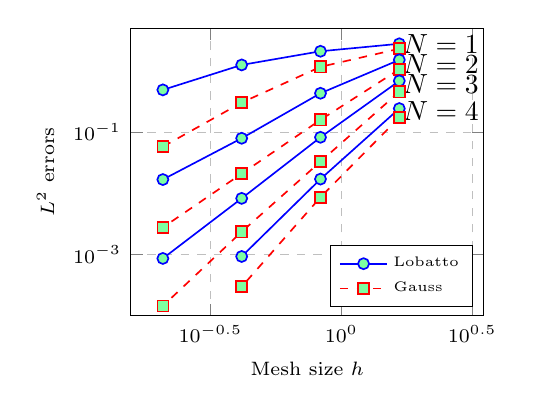
\begin{tikzpicture}
\begin{loglogaxis}[
    width=.5\textwidth,
    xlabel={Mesh size $h$},
    ylabel={$L^2$ errors}, 
    xmax=3.5,
    ymin=1e-4, ymax=5,
    legend pos=south east, legend cell align=left, legend style={font=\tiny},	
    xmajorgrids=true, ymajorgrids=true, grid style=dashed,
    legend entries={Lobatto, Gauss}
]
\pgfplotsset{
cycle list={{blue, mark=*}, {red, dashed ,mark=square*}}
}
\addplot+[semithick, mark options={solid, fill=markercolor}]
coordinates{(1.66667,2.78317)(0.833333,2.09894)(0.416667,1.25478)(0.208333,0.490133)};
%\addplot+[semithick, mark options={solid, fill=markercolor}]
%coordinates{(1.66667,2.81566)(0.833333,2.2122)(0.416667,1.44626)(0.208333,0.801638)};
\addplot+[semithick, mark options={solid, fill=markercolor}]
coordinates{(1.66667,2.30772)(0.833333,1.16697)(0.416667,0.303428)(0.208333,0.0576807)};

% N = 2
\addplot+[semithick, mark options={solid, fill=markercolor}]
coordinates{(1.66667,1.51766)(0.833333,0.431437)(0.416667,0.0792017)(0.208333,0.0167253)};
%\addplot+[semithick, mark options={solid, fill=markercolor}]
%coordinates{(1.66667,1.52643)(0.833333,0.436466)(0.416667,0.0801575)(0.208333,0.0167043)};
\addplot+[semithick, mark options={solid, fill=markercolor}]
coordinates{(1.66667,1.06169)(0.833333,0.158534)(0.416667,0.0208737)(0.208333,0.00274974)};

% N = 3
\addplot+[semithick, mark options={solid, fill=markercolor}]
coordinates{(1.66667,0.68797)(0.833333,0.0821894)(0.416667,0.008229)(0.208333,0.000856128)};
%\addplot+[semithick, mark options={solid, fill=markercolor}]
%coordinates{(1.66667,0.685655)(0.833333,0.0815906)(0.416667,0.00838271)(0.208333,0.000889147)};
\addplot+[semithick, mark options={solid, fill=markercolor}]
coordinates{(1.66667,0.455651)(0.833333,0.0328805)(0.416667,0.00233608)(0.208333,0.000143112)};

% N = 4
\addplot+[semithick, mark options={solid, fill=markercolor}]
coordinates{(1.66667,0.242584)(0.833333,0.0170238)(0.416667,0.000922618)};
%\addplot+[semithick, mark options={solid, fill=markercolor}]
%coordinates{(1.66667,0.241312)(0.833333,0.0169965)(0.416667,0.000928106)};
\addplot+[semithick, mark options={solid, fill=markercolor}]
coordinates{(1.66667,0.173237)(0.833333,0.00858261)(0.416667,0.00029501)};

\node at (axis cs:2.4,2.8) {$N = 1$};
\node at (axis cs:2.4,1.3) {$N = 2$};
\node at (axis cs:2.4,.6) {$N = 3$};
\node at (axis cs:2.4,.22) {$N = 4$};
\end{loglogaxis}
\end{tikzpicture}
}
}
\only<2>{
\subfloat[Coarse non-conforming mesh]{\raisebox{3em}{\includegraphics[width=.425\textwidth]{figs/noncon_curved_mesh.png}}}
\hspace{.25em}
\subfloat[Sub-optimal rates if under-integrated]{
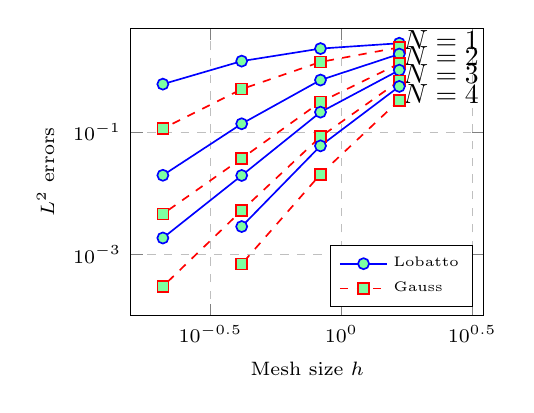
\begin{tikzpicture}
\begin{loglogaxis}[
    width=.5\textwidth,
    xlabel={Mesh size $h$},
    ylabel={$L^2$ errors}, 
    xmax=3.5,
    ymin=1e-4, ymax=5,
    legend pos=south east, legend cell align=left, legend style={font=\tiny},	
    xmajorgrids=true, ymajorgrids=true, grid style=dashed,
    legend entries={Lobatto, Gauss}%, Lobatto-Gauss}    
]
\pgfplotsset{
cycle list={{blue, mark=*}, {red, dashed ,mark=square*}}%,{black, dashdotted ,mark=triangle*}}
}
% N = 1
\addplot+[semithick, mark options={solid, fill=markercolor}]
coordinates{(1.66667,2.84018)(0.833333,2.32278)(0.416667,1.44878)(0.208333,0.608642)};
%\addplot+[semithick, mark options={solid, fill=markercolor}]
%coordinates{(1.66667,2.8287)(0.833333,2.36062)(0.416667,1.61841)(0.208333,0.909621)};
\addplot+[semithick, mark options={solid, fill=markercolor}]
coordinates{(1.66667,2.42938)(0.833333,1.40381)(0.416667,0.504184)(0.208333,0.114213)};

% N = 2
\addplot+[semithick, mark options={solid, fill=markercolor}]
coordinates{(1.66667,1.88997)(0.833333,0.710146)(0.416667,0.136728)(0.208333,0.0196411)};
%\addplot+[semithick, mark options={solid, fill=markercolor}]
%coordinates{(1.66667,1.88857)(0.833333,0.709214)(0.416667,0.135323)(0.208333,0.0196621)};
\addplot+[semithick, mark options={solid, fill=markercolor}]
coordinates{(1.66667,1.32118)(0.833333,0.310973)(0.416667,0.0369794)(0.208333,0.00457492)};

% N = 3
\addplot+[semithick, mark options={solid, fill=markercolor}]
coordinates{(1.66667,1.03021)(0.833333,0.211902)(0.416667,0.0195018)(0.208333,0.00184924)};
%\addplot+[semithick, mark options={solid, fill=markercolor}]
%coordinates{(1.66667,1.03557)(0.833333,0.211255)(0.416667,0.0196214)(0.208333,0.0018744)};
\addplot+[semithick, mark options={solid, fill=markercolor}]
coordinates{(1.66667,0.6875)(0.833333,0.0837258)(0.416667,0.0052072)(0.208333,0.000298318)};

% N = 4
\addplot+[semithick, mark options={solid, fill=markercolor}]
coordinates{(1.66667,0.558299)(0.833333,0.0594828)(0.416667,0.00284697)};
%\addplot+[semithick, mark options={solid, fill=markercolor}]
%coordinates{(1.66667,0.557251)(0.833333,0.0593767)(0.416667,0.00284163)};
\addplot+[semithick, mark options={solid, fill=markercolor}]
coordinates{(1.66667,0.330743)(0.833333,0.0204084)(0.416667,0.000691875)};

\node at (axis cs:2.4,3.25) {$N = 1$};
\node at (axis cs:2.4,1.75) {$N = 2$};
\node at (axis cs:2.4,.9) {$N = 3$};
\node at (axis cs:2.4,.425) {$N = 4$};
\end{loglogaxis}
\end{tikzpicture}
}
}
\end{figure}

\begin{center}
The skew symmetric formulation is entropy stable for both Lobatto and Gauss quadrature, but Lobatto is $O(h^N)$ while Gauss is $O(h^{N+1})$.
\end{center}

\let\thefootnote\relax\footnotetext{\tiny Chan (2019). \textit{Skew-symmetric entropy stable modal discontinuous Galerkin formulations}.}
}



%% =================================================

\subsection{Reduced order modeling}

\frame[noframenumbering]{
\frametitle{Talk outline}
\tableofcontents[currentsection,currentsubsection]
}

\frame{
\frametitle{Projection-based reduced order models (ROMs)}
\vspace{-.5em}
\begin{figure}
\centering
\includegraphics[width=.65\textwidth]{figs/POD_illustration.png}
\end{figure}
\vspace{-.5em}
\begin{itemize}
\item Goal: reduce cost of many-query scenarios (design space exploration).
\item Main steps: \note{offline} training phase with full order model (FOM), cheap \note{online} phase with reduced order model (ROM).
\end{itemize} 

\uncover<2>{
\begin{center}
\minibox[frame]{Challenge: ROMs inherit stability of FOM for elliptic PDEs,\\
but not for nonlinear hyperbolic problems!}
\end{center}
}

\let\thefootnote\relax\footnotetext{\tiny Figure adapted from Brunton, Proctor, Kutz (2016), \textit{Discovering governing equations from data \ldots}.}
}

\frame{
\frametitle{Full order model: entropy stable finite volumes}
\vspace{-.75em}
\begin{figure}
\centering
\includegraphics[width=.6\textwidth]{figs/fv_illustration.png}
\end{figure}
\vspace{-1.25em}
\begin{itemize}
\item Discretize integrated form of nonlinear conservation law
\[
\Delta x \td{\bm{u}_i}{t} + {\bm{f}_{S}(\bm{u}_{i+1},\bm{u}_i) - \bm{f}_{S}(\bm{u}_{i},\bm{u}_{i-1})} = 0, \qquad \text{interior } i. 
\]
\item Matrix formulation: let $\bm{M} = (\Delta x) \bm{I}$, and (assuming periodicity)
\[
\bm{M}\td{\bm{u}}{t} + 2\LRp{\bm{Q}\circ \bm{F}}\bm{1} + \underbrace{\epsilon\bm{K}\bm{u}}_{\text{art.\ viscosity}} = 0, \qquad \bm{Q} =\frac{1}{2} \begin{bmatrix}
0 & 1 & & -1\\
-1 & 0 & 1 &\\
& \ddots & \ddots & 1 \\
1 & & -1  & 0
\end{bmatrix}
\]
\end{itemize}
}

\frame{
\frametitle{Naive POD-Galerkin procedure}
\begin{itemize}
\item (Offline) compute POD basis from solution component snapshots.
\[
\bm{V} = {\begin{bmatrix} \vertbar & & \vertbar \\
\phi_1 & \ldots & \phi_N\\
\vertbar & & \vertbar
\end{bmatrix}}, \qquad \phi_i^T\phi_j =0, \qquad \bm{u} \approx \bm{V} \bm{u}_N.
\]
\item (Online) Galerkin projection of the matrix system 
\[
{\bm{V}^T\bm{M}\bm{V}} \td{\bm{u}_N}{t} + 2\bm{V}^T \LRp{{\bm{Q}}\circ \bm{F}}\bm{1} = 0.
\]
\item (Online) Entropy projection results in an entropy stable ROM
\begin{gather*}
{\tilde{\bm{u}} = \bm{u}\LRp{\bm{V} \bm{V}^{\dagger} \bm{v}\LRp{\bm{V} \bm{u}_N}}}, \qquad \LRp{\bm{F}}_{ij} = \bm{f}_S\LRp{\tilde{\bm{u}}_i,\tilde{\bm{u}}_j}.
\end{gather*}
For accuracy, compute POD basis from snapshots of both conservative and entropy variables.  
\end{itemize}
}

\frame{
\frametitle{Evaluating nonlinear ROM terms dominates costs}
\vspace{-.75em}
\begin{center}
Problem: cost of evaluating ROM nonlinear terms scales with\\
\note{number of grid points}!  Cost still scales with size of full order model.
\[
{\tilde{\bm{u}} = \note{\bm{u}}\LRp{\bm{V} \bm{V}^\dagger \note{\bm{v}}\LRp{\bm{V} \bm{u}_N}}}, \qquad 2\LRp{{\bm{Q}}\circ \note{\bm{F}}}\bm{1} 
\]
\end{center}
\vspace{-1em}
\uncover<2->{
\begin{columns}
\begin{column}{.55\textwidth}
\begin{itemize}
\item \note{Hyper-reduction} reduces costs by approximating nonlinear evaluations.  
\begin{overlayarea}{\textwidth}{.275\textheight}
\vspace{-.75em}
\begin{align*}
&\bm{V}^T\bm{g}(\bm{V}\bm{u}_N) \approx\\
&\only<1-2>{\underbrace{\bm{V}(\mathcal{I},:)^T}_{\text{sampled rows}}\bm{W}\bm{g}(\bm{V}(\mathcal{I},:)\bm{u}_N)}
\only<3>{\bm{V}(\mathcal{I},:)^T\underbrace{\bm{W}}_{\substack{\text{diag}\\ \text{weights}}}\bm{g}(\bm{V}(\mathcal{I},:)\bm{u}_N)}
\end{align*}
\end{overlayarea}
\item Examples: gappy POD, DEIM, empirical cubature, ECSW, \ldots
\end{itemize}
\end{column}
}
\begin{column}{.45\textwidth}
\begin{figure}
%\centering
\begin{overlayarea}{\textwidth}{.5\textheight}
\only<1>{\includegraphics[width = .8\textwidth]{figs/hyperreduc_illustration0.png}}
\only<2->{\includegraphics[width = .8\textwidth]{figs/hyperreduc_illustration.png}}
\end{overlayarea}
\end{figure}
\end{column}
\end{columns}

\let\thefootnote\relax\footnotetext{\tiny Hernandez et al., An et al., Bui/Willcox, Chantarantabut /Sorensen, Drmac/Gugercin, Farhat et al.\, Patera/Yano, \ldots}
}

\frame{
\frametitle{Entropy stability and standard hyper-reduction}

\begin{itemize}
\item How to hyper-reduce $\LRp{\bm{Q}\circ \bm{F}}$?  Construct a \textit{sampled} matrix $\bm{Q}_s$ from $\bm{Q}$.  Need \note{$\bm{Q}_s = -\bm{Q}_s^T$} and \note{$\bm{Q}_s\bm{1} = \bm{0}$} for entropy stability.
\vspace{2em}
\item Options: sub-sample rows and columns of full matrix $\bm{Q}$ or approximate $\bm{Q}$ by weighted sum of local skew matrices $\bm{Q}_e$.  
\[
\bm{Q} = \sum_{e=1}^K \bm{Q}_e \approx \bm{Q}_s = \sum_{e = 1}^K \bm{w}_e \bm{Q}_e, \qquad \bm{w} \text{ sparse}.
\]
\uncover<2->{Problems: either \note{$\bm{Q}_s$ loses skew-symmetry} or \note{$\bm{Q}_s\bm{1}\neq \bm{0}$}.}
%\vspace{1.5em}
%\item<5-> Project $\bm{Q}$ onto reduced basis $\bm{V}^T\bm{Q} \bm{V}$.
\end{itemize}

\let\thefootnote\relax\footnotetext{\tiny Patera and Yano (2017). \textit{An LP empirical quadrature procedure for parametrized functions}.}
}


\frame{
\frametitle{Two-step hyper-reduction: compress and project}
%\begin{overlayarea}{\textwidth}{\textheight}
%\vspace{1em}
\begin{itemize}
\item<1-> Step 1: construct a \textit{modal} $\bm{Q}$ using an expanded ``test'' basis $\bm{V}_t$
\[
\bm{V}_t^T\bm{Q}\bm{V}_t, \qquad \bm{1}\in \mathcal{R}\LRp{\bm{V}_t}
% = {\rm orth}\LRp{
%\begin{bmatrix} 
%\bm{V} & \bm{1}
%\end{bmatrix}}
\]
%\vspace{1em}
\item<2-> Step 2: determine test basis coefficients using hyper-reduced points.  
%\item<2-> Compute \note{empirical cubature} points + projection for $\bm{Q}_s$
\begin{gather*}
%\bm{W}_{ij} = w_{ii}\delta_{ij}, \quad 
\bm{M}_t = \bm{V}_t(\mathcal{I},:)^T\bm{W}\bm{V}_t(\mathcal{I},:), \qquad \bm{P}_t = \bm{M}_t^{-1}\bm{V}_t(\mathcal{I},:)^T\bm{W}.%, \qquad \text{ discrete projection}
%\bm{Q}_s = \bm{P}_t^T \LRp{\bm{V}_t^T\bm{Q}\bm{V}_t} \bm{P}_t. 
\end{gather*}
Here, $\bm{P}_t$ is a weighted projection onto the test basis.  %(can also use Gappy POD).
%\item<2-> Compression + sampling ensure $\bm{Q}_t\bm{1} = 0$ and $\bm{Q}_t = -\bm{Q}_t^T$ (on periodic domains) for entropy stability.
%\[
%\underbrace{\bm{V}(\mathcal{I},:)^T\bm{W}\bm{V}(\mathcal{I},:)}_{\bm{M}_N} \td{\bm{u}_N}{t} + \bm{V}(\mathcal{I},:)^T \LRp{\bm{Q}_t\circ \bm{F}}\bm{1} = 0.
%\]
\vspace{1em}
\item<3-> Step 3 (combine Steps 1 and 2): define 
\[
\bm{Q}_s = \bm{P}_t^T\LRp{\bm{V}_t^T\bm{Q}\bm{V}_t}\bm{P}_t
\]
Then, $\bm{Q}_s = -\bm{Q}_s^T$ and $\bm{Q}_s\bm{1} = \bm{0}$!
\end{itemize}
%\end{overlayarea}

\let\thefootnote\relax\footnotetext{\tiny Hernandez, Caicedo, Ferrer (2017).  \textit{Dimensional hyper-reduction of nonlinear finite element models via empirical cubature.}}
%\let\thefootnote\relax\footnotetext{\tiny Everson, Sirovich (1995).  \textit{Karhunen--Loeve procedure for gappy data.}}
}

\frame{
\begin{itemize}
\item Problem: modes $\bm{V}_t$ may sample $\bm{Q}\bm{V}$ very poorly, e.g., $\bm{V}_t^T\bm{Q}\bm{V}_t\approx \bm{0}$!
\vspace{-1.5em}
\begin{figure}
\centering
\subfloat[\scriptsize Shock snapshots]{\includegraphics[width=.3\textwidth]{figs/burg_snaps.png}}
\hspace{.1em}
\subfloat[\scriptsize Modes (columns of $\bm{V}$)]{\includegraphics[width=.3\textwidth]{figs/burg3modes.png}}
\hspace{.1em}
\subfloat[\scriptsize Mode derivatives $\bm{Q}\bm{V}$]{\includegraphics[width=.3\textwidth]{figs/burg3modes_diff.png}}
\end{figure}
\vspace{.5em}
\item Fix: sample $\bm{Q}$ using an expanded ``test'' basis $\bm{V}_t$ 
\begin{gather*}
\bm{V}_t = {\rm orth}\LRp{
\begin{bmatrix} 
\bm{V} & \bm{1} & \bm{Q}\bm{V} 
\end{bmatrix}}, \qquad
\bm{V}_t^T\bm{Q}\bm{V}_t \in \mathbb{R}^{(2N+1) \times (2N+1)}. %\mathbb{R}^{(d+1)N+1 \times (d+1)N+1}.
\end{gather*}
$\bm{Q}_s = \bm{P}_t^T\LRp{\bm{V}_t^T\bm{Q}\bm{V}_t}\bm{P}_t$ is now accurate, $\bm{Q}_s = -\bm{Q}_s^T$, and $\bm{Q}_s\bm{1} = \bm{0}$.
\end{itemize}

\let\thefootnote\relax\footnotetext{\tiny Carlberg, Barone, Antil (2017).  \textit{Galerkin v. least-squares Petrov--Galerkin projection in nonlinear model reduction.}}
}

\frame{
\frametitle{Hyper-reduction: empirical cubature}

\begin{itemize}
\item Greedy algorithm constructs an approximate quadrature which integrates a target space to some tolerance.
\vspace{1em}
\item Target space motivated by inner products of POD basis: most accurate + smallest number of points in practice
\[
\text{Target space } = {\rm span}\LRc{\phi_i(\bm{x})\phi_j(\bm{x}), \quad 1\leq i,j \leq N}.
\]
%\vspace{.01em}
\item<2-> Problem: target space ignores rest of expanded test basis.  Test mass matrix $\bm{M}_t$ may be \note{singular} $\Longrightarrow$ projection matrix $\bm{P}_t$ ill-defined!  
\vspace{1em}
\item<3> Fix: add \note{``stabilizing'' points} which target the near null space of $\bm{M}_t$.  
\end{itemize} 

\let\thefootnote\relax\footnotetext{\tiny An, Kim, James (2009).  \textit{Optimizing cubature for efficient integration of subspace deformations}.}
\let\thefootnote\relax\footnotetext{\tiny Hernandez, Caicedo, Ferrer (2017).  \textit{Dimensional hyper-reduction of nonlinear finite element models via empirical cubature.}}
}

\frame{
\frametitle{Summary: entropy stable ROMs on periodic domains}

%\note{Summarize here}
\vspace{-.25em}
\begin{itemize}
\item Two-step hyper-reduction of $\LRp{\bm{Q}\circ \bm{F}}$: compress and project
\begin{itemize}
\item Compress $\bm{Q}$ onto expanded test basis spanning $\bm{1}$, $\bm{V}$, and $\bm{Q}\bm{V}$.
\item Project hyper-reduced point values onto modes of test basis 
\[
\bm{Q}_s = \bm{P}_t^T\LRp{\bm{V}_t^T\bm{Q}\bm{V}_t}\bm{P}_t
\]
%Reduced $\bm{Q}_s$ satisfies $\bm{Q}_s\bm{1} = \bm{0}$ and $\bm{Q}_s = -\bm{Q}_s^T$.
\end{itemize}
%\vspace{1em}
\item Entropy stable reduced order model with hyper-reduction:
\begin{gather*}
{\bm{V}(\mathcal{I},:)^T\bm{W}\bm{V}(\mathcal{I},:)} \td{\bm{u}_N}{t} + 2\bm{V}(\mathcal{I},:)^T \LRp{\bm{Q}_s\circ \bm{F}}\bm{1} = 0,\\
%\underbrace{\bm{V}(\mathcal{I},:)^T\bm{W}\bm{V}(\mathcal{I},:)}_{\bm{M}_N} \td{\bm{u}_N}{t} + \bm{V}(\mathcal{I},:)^T \LRp{\bm{Q}_s\circ \bm{F}}\bm{1} = 0.
%{\bm{V}(\mathcal{I},:)^T\bm{W}\bm{V}(\mathcal{I},:)} \td{\bm{u}_N}{t} + \bm{V}(\mathcal{I},:)^T \LRp{\bm{Q}_s\circ \bm{F}}\bm{1} = 0,\\
{\bm{F}}_{ij} = \bm{f}_S\LRp{\tilde{\bm{u}}_i,\tilde{\bm{u}}_j}, \quad \tilde{\bm{u}} = \bm{u}\LRp{\bm{V}(\mathcal{I},:)\bm{P} \bm{v}\LRp{\bm{V}\bm{u}_N}},
%\LRp{\bm{V}(\mathcal{I},:)^T\bm{W}\bm{V}(\mathcal{I},:)}^{-1}{\bm{V}(\mathcal{I},:)^T\bm{W}}.
\end{gather*}
where $\bm{P}$ is the hyper-reduced projection onto POD modes.
\vspace{.75em}
\item<2-> No free lunch: $\note{O(N_s^2)}$ vs $O(N_s)$ flux evaluations, where $N_s = |\mathcal{I}|$.
\end{itemize}
}

\frame{
\frametitle{Non-periodic boundary conditions}

\begin{itemize}
%\item Non-periodic domains: full order matrix $\bm{Q}$ is \textit{nearly} skew-symmetric
%\[
%\bm{Q} = \bm{S} + \bm{B}, \qquad \bm{S} = \begin{bmatrix} 
% 0& 1 & 0\\
%-1& 0 &1\\
%0& -1 & 0
%\end{bmatrix}, \qquad \bm{B} = \begin{bmatrix} -1 & &\\
%&0&\\
%&&1
%\end{bmatrix}
%\]
\item Weak boundary conditions using hybridized SBP operators + DG numerical flux.  
\vspace{1em}
\item Can add entropy-dissipative penalization terms (e.g., Lax-Friedrichs).
%\[
%\bm{Q}_h = \begin{bmatrix}
%\bm{Q}-\bm{Q}^T & \bm{E}^T\bm{B}\\
%-\bm{B}\bm{E} & 
%\end{bmatrix}
%\]
\vspace{1em}
\item In 2D/3D, entropy stability requires surface quad.\ weights $\bm{w}_f$ to satisfy weak SBP property involving surface interpolation matrix $\bm{V}_f$.  
\begin{align*}
\bm{V}_t^T \bm{Q}_x^T\bm{1} &= \bm{V}_f^T \LRp{\bm{n}_x \circ \note{\bm{w}_f}},\\
\bm{V}_t^T \bm{Q}_y^T\bm{1} &= \bm{V}_f^T \LRp{\bm{n}_y \circ \note{\bm{w}_f}}.
\end{align*}
Enforce conditions using constrained LP hyper-reduction.
\end{itemize}

\let\thefootnote\relax\footnotetext{\tiny Patera and Yano (2017). \textit{An LP empirical quadrature procedure for parametrized functions}.}
\let\thefootnote\relax\footnotetext{\tiny Chan (2018). \textit{On discretely entropy conservative and entropy stable discontinuous Galerkin methods.}}
\let\thefootnote\relax\footnotetext{\tiny Chan (2019). \textit{Skew-symmetric entropy stable modal discontinuous Galerkin formulations}.}
}


\frame{
\frametitle{1D Euler with reflective BCs + shock}
\setcounter{subfigure}{0}
\vspace{-1em}
\begin{figure}
\centering 
\only<1>{
\subfloat[25 modes, $T=.25$]{\includegraphics[width=.45\textwidth]{figs/euler1Dwall_t25_25modes.png}}
\hspace{.5em}
\subfloat[25 modes, $T=.75$]{\includegraphics[width=.45\textwidth]{figs/euler1Dwall_t75_25modes.png}}
\caption*{\footnotesize FOM with $2500$ grid points, viscosity coefficient $\epsilon = 2e-4$, ROM with 25 modes.}
}
\only<2>{
\subfloat[75 modes, $T=.25$]{\includegraphics[width=.45\textwidth]{figs/euler1Dwall_t25_75modes.png}}
\hspace{.5em}
\subfloat[75 modes, $T=.75$]{\includegraphics[width=.45\textwidth]{figs/euler1Dwall_t75_75modes.png}}
\caption*{\footnotesize FOM with $2500$ grid points, viscosity coefficient $\epsilon = 2e-4$, ROM with 75 modes.}
}
\only<3>{
\subfloat[125 modes, $T=.25$]{\includegraphics[width=.45\textwidth]{figs/euler1Dwall_t25_125modes.png}}
\hspace{.5em}
\subfloat[125 modes, $T=.75$]{\includegraphics[width=.45\textwidth]{figs/euler1Dwall_t75_125modes.png}}
\caption*{\footnotesize FOM with $2500$ grid points, viscosity coefficient $\epsilon = 2e-4$, ROM with 125 modes.}
}
\end{figure}
\vspace{-.5em}
\begin{table}[!h]
\centering
\begin{tabular}{|c || c | c | c |c |}
\hline
Number of modes $N$ & 25 & 75 & 125 & 175\\
\hhline{|=|=|=|=|=|}
Number of empirical cubature points &54 & 158 & 259 &355 \\
\hline
Number of stabilizing points & 3& 21 & 36 & 28 \\
%\hline
%Number of viscous points & 54 &159 & 259 & 366  \\
\hline
\end{tabular}
%\caption{Number of computed hyper-reduced points for the 1D Euler equations.}
\label{tab:hrpts}
\end{table}
%\begin{center}
%All results use explicit RK-45 time-stepping with FOM time-step.
%\end{center}
}

\frame{
\frametitle{Entropy conservation test}
\begin{figure}[!h]
\centering
\subfloat[Density $\rho$ (125 modes, no viscosity)]{\includegraphics[width=.45\textwidth]{euler1Dwall_t75_125modes_novisc.png}}
\hspace{1em}
\subfloat[Convective entropy contribution]{\includegraphics[width=.47\textwidth]{entropyrhs.png}}
%\subfloat[Difference, 25 modes]{\includegraphics[width=.32\textwidth]{viscdiff25modes.png}}
\caption{Reduced order solution and convective entropy RHS contribution $\LRb{\bm{v}_N^T \bm{V}_h^T\LRp{\bm{Q}_h \circ \bm{F}}\bm{1}}$ for the case of zero viscosity.}
\label{fig:novisc}
\end{figure}
}

\frame{
\frametitle{Evolution of average entropy}

\begin{figure}
\centering 
\only<1>{
\includegraphics[width=.7\textwidth]{figs/euler1Dwall_entropy_25modes.png}
\caption*{Average entropy over time (25 modes).}
}
\only<2>{
\includegraphics[width=.7\textwidth]{figs/euler1Dwall_entropy_75modes.png}
\caption*{Average entropy over time (75 modes).}
}
\only<3>{
\includegraphics[width=.7\textwidth]{figs/euler1Dwall_entropy_125modes.png}
\caption*{Average entropy over time (125 modes).}
}
\end{figure}
}

\frame{
\frametitle{Error with and without hyper-reduction}
\vspace{-.5em}
\begin{figure}
\centering
\includegraphics[width=.65\textwidth]{figs/euler_error_hypred_comparison_K2500.png}
\caption{Error over time for a $K=2500$ FOM and ROM with $25, 75, 125$ modes.}
\end{figure}
}

\frame{
\frametitle{Smoothed 2D Kelvin-Helmholtz instability}
\vspace{-.5em}
\begin{figure}
\centering 
\only<1>{
\subfloat[Density, full order model]{\includegraphics[width=.45\textwidth]{figs/khfom.png}}
\hspace{.5em}
\subfloat[Reduced order model]{\includegraphics[width=.45\textwidth]{figs/khrom75.png}}
}
\only<2>{
\subfloat[Density, full order model]{\includegraphics[width=.45\textwidth]{figs/khfom.png}}
\hspace{.5em}
\subfloat[ROM w/reduced quad.\ points]{\includegraphics[width=.45\textwidth]{figs/khrom75_hrpts.png}}
}
\caption{Full order model with $40000$ points, viscosity $\epsilon = .5\Delta x$.  ROM with $75$ modes, $865$ reduced quadrature points, $1.11 \%$ relative $L^2$ error at $T = 3$.}
\end{figure}
}

\frame{
\frametitle{2D Gaussian pulse with reflective wall}

\begin{figure}
\centering 
\only<1>{
\subfloat[Density, full order model]{\includegraphics[width=.45\textwidth]{figs/pulse2d.png}}
\hspace{.5em}
\subfloat[Reduced order model]{\includegraphics[width=.45\textwidth]{figs/pulse2d_ROM.png}}
}
\only<2>{
\subfloat[Density, full order model]{\includegraphics[width=.45\textwidth]{figs/pulse2d.png}}
\hspace{.5em}
\subfloat[ROM w/reduced quad.\ points]{\includegraphics[width=.4525\textwidth]{figs/pulse2d_ROM_pts.png}}
}
\caption{FOM with $10000$ points, viscosity $\epsilon = .5\Delta x$.  ROM with $25$ modes, $306$ reduced volume points, 82 reduced surface points, $.57 \%$ error at $T = .25$.}
\end{figure}

}
%
%
%\frame{
%\frametitle{Evaluating nonlinear ROM terms dominates costs}
%\vspace{-.5em}
%\begin{center}
%Problem: cost of evaluating ROM nonlinear terms scales with\\
%\note{number of grid points (squared)}!  No improvement over full order model.
%\[
%{\tilde{\bm{u}} = \note{\bm{u}}\LRp{\bm{V} \bm{V}^T \note{\bm{v}}\LRp{\bm{V} \bm{u}_N}}}, \qquad \LRp{{\bm{Q}}\circ \note{\bm{F}}}\bm{1} 
%\]
%\end{center}
%\vspace{-.75em}
%\uncover<2>{
%\begin{columns}
%\begin{column}{.55\textwidth}
%\begin{itemize}
%\item \note{Hyper-reduction} reduces costs by approximating nonlinear evaluations.  
%\begin{align*}
%&\bm{V}^T\bm{g}(\bm{V}\bm{u}_N) \approx\\
%&\underbrace{\bm{V}(\mathcal{I},:)^T}_{\text{sampled rows}}\bm{W}\bm{g}(\bm{V}(\mathcal{I},:)\bm{u}_N)
%\end{align*}
%%\vspace{1.5em}
%\item Examples: gappy POD, DEIM, empirical cubature, ECSW, \ldots
%\end{itemize}
%\end{column}
%}
%\begin{column}{.45\textwidth}
%\begin{figure}
%%\centering
%\begin{overlayarea}{\textwidth}{.5\textheight}
%\only<1>{\includegraphics[width = .8\textwidth]{figs/hyperreduc_illustration0.png}}
%\only<2>{\includegraphics[width = .8\textwidth]{figs/hyperreduc_illustration.png}}
%\end{overlayarea}
%\end{figure}
%\end{column}
%\end{columns}
%
%\let\thefootnote\relax\footnotetext{\tiny Hernandez et al., An et al., Bui/Willcox, Chantarantabut /Sorensen, Drmac/Gugercin, Farhat et al.\, Patera/Yano, \ldots}
%}
%
%\frame{
%\frametitle{Hyper-reduction through empirical cubature}
%
%\begin{itemize}
%\item<1-> (Offline) compress $\bm{Q}$ using orthonormal ``test'' basis $\bm{V}_t$
%\begin{gather*}
%\bm{V}_t = {\rm orth}\LRp{
%\begin{bmatrix} 
%\bm{V} & \bm{Q}\bm{V} & \bm{1}
%\end{bmatrix}}, \qquad
%\bm{V}_t^T\bm{Q}\bm{V}_t \in \mathbb{R}^{(2N+1) \times (2N+1)}. %\mathbb{R}^{(d+1)N+1 \times (d+1)N+1}.
%\end{gather*}
%%Reduced operator $\tilde{\bm{Q}}_N$ is skew-symmetric and satisfies $\tilde{\bm{Q}}_N\bm{1} = 0$.
%%\item Greedy algorithm for  approx.\ of $\int \phi_i(\bm{x}) \phi_j(\bm{x})$.  
%\item<2-> (Offline) compute \note{empirical cubature}, projection, and reduced $\bm{Q}_t$
%\begin{gather*}
%\bm{W}_{ij} = w_{ii}\delta_{ij},  \qquad \bm{M}_t = \bm{V}_t(\mathcal{I},:)^T\bm{W}\bm{V}_t(\mathcal{I},:)\\
%\bm{P}_t = \bm{M}_t^{-1}\bm{V}_t(\mathcal{I},:)^T\bm{W}, \qquad
%\bm{Q}_t = \bm{P}_t^T \LRp{\bm{V}_t^T\bm{Q}\bm{V}_t} \bm{P}_t. 
%\end{gather*}
%\item<3-> Compression + sampling strategies ensure that $\bm{Q}_t\bm{1} = 0$ and $\bm{Q}_t = -\bm{Q}_t^T$ (periodic domains) for entropy stability.
%\[
%\underbrace{\bm{V}(\mathcal{I},:)^T\bm{W}\bm{V}(\mathcal{I},:)}_{\bm{M}_N} \td{\bm{u}_N}{t} + \bm{V}(\mathcal{I},:)^T \LRp{\bm{Q}_t\circ \bm{F}}\bm{1} = 0.
%\]
%\end{itemize}
%
%\let\thefootnote\relax\footnotetext{\tiny An, Kim, James (2009).  \textit{Optimizing cubature for efficient integration of subspace deformations}.}
%\let\thefootnote\relax\footnotetext{\tiny Hernandez, Caicedo, Ferrer (2017).  \textit{Dimensional hyper-reduction of nonlinear finite element models via empirical cubature.}}
%}
%
%
%\frame{
%\frametitle{Numerical results: 1D Euler with reflective BCs + shock}
%\setcounter{subfigure}{0}
%\vspace{-1em}
%\begin{figure}
%\centering 
%\only<1>{
%\subfloat[25 modes, 100 ECP, $T=.25$]{\includegraphics[width=.45\textwidth]{figs/euler1Dwall_t25_25modes.png}}
%\hspace{.5em}
%\subfloat[25 modes, 100 ECP, $T=.75$]{\includegraphics[width=.45\textwidth]{figs/euler1Dwall_t75_25modes.png}}
%\caption*{\footnotesize FOM with $2500$ grid points, viscosity coefficient $\epsilon = 2e-4$, ROM with 25 modes.}
%}
%\only<2>{
%\subfloat[75 modes, 205 ECP, $T=.25$]{\includegraphics[width=.45\textwidth]{figs/euler1Dwall_t25_75modes.png}}
%\hspace{.5em}
%\subfloat[75 modes, 205 ECP, $T=.75$]{\includegraphics[width=.45\textwidth]{figs/euler1Dwall_t75_75modes.png}}
%\caption*{\footnotesize FOM with $2500$ grid points, viscosity coefficient $\epsilon = 2e-4$, ROM with 75 modes.}
%}
%\only<3>{
%\subfloat[125 modes, 304 ECP, $T=.25$]{\includegraphics[width=.45\textwidth]{figs/euler1Dwall_t25_125modes.png}}
%\hspace{.5em}
%\subfloat[125 modes, 304 ECP, $T=.75$]{\includegraphics[width=.45\textwidth]{figs/euler1Dwall_t75_125modes.png}}
%\caption*{\footnotesize FOM with $2500$ grid points, viscosity coefficient $\epsilon = 2e-4$, ROM with 125 modes.}
%}
%\end{figure}
%
%\begin{center}
%Non-periodic boundary conditions treated using hybridized SBP operators and constrained hyper-reduction (to enforce weak SBP property).  
%\end{center}
%
%\let\thefootnote\relax\footnotetext{\tiny Patera and Yano (2017). \textit{An LP empirical quadrature procedure for parametrized functions}.}
%}
%
%\frame{
%\frametitle{Numerical results: smoothed Kelvin-Helmholtz instability}
%\vspace{-.5em}
%\begin{figure}
%\centering 
%\only<1>{
%\subfloat[Full order model]{\includegraphics[width=.45\textwidth]{figs/khfom.png}}
%\hspace{.5em}
%\subfloat[Reduced order model, 75 modes]{\includegraphics[width=.45\textwidth]{figs/khrom_75.png}}
%}
%\only<2>{
%\subfloat[Full order model]{\includegraphics[width=.45\textwidth]{figs/khfom.png}}
%\hspace{.5em}
%\subfloat[ROM w/reduced quad.\ points]{\includegraphics[width=.45\textwidth]{figs/khrom_75_ecp989.png}}
%}
%\caption{Full order model with $10000$ points, viscosity $\epsilon = 1e-3$, $T = 2.5$.  ROM with $75$ modes, $989$ reduced quadrature points, $1.15 \%$ relative $L^2$ error.}
%\end{figure}
%
%}


%% =================================================

\frame{
\frametitle{Summary and future work}

\begin{itemize}
\item Entropy stable modal formulations are flexible, with applications to simplicial elements, tensor product elements, and ROMs.
%\vspace{.25em}
%\item Current work: ROM, positivity preservation.  
\vspace{.25em}
%\item Current work: hybrid and non-conforming meshes, multi-GPU.
%\vspace{.25em}
\item This work is supported by DMS-1719818 and DMS-1712639. 
\end{itemize}
\vspace{.25em}
\begin{center}
Thank you!  Questions?
\vspace{.25em}

{\includegraphics[width=.15\textwidth]{figs/nsf.jpg}}
\end{center}

\let\thefootnote\relax\footnotetext{\tiny Chan (2019). \textit{Entropy stable reduced order modeling of nonlinear conservation laws}.}
\let\thefootnote\relax\footnotetext{\tiny Chan (2019). \textit{Skew-symmetric entropy stable modal discontinuous Galerkin formulations}.}
\let\thefootnote\relax\footnotetext{\tiny Chan, Del Rey Fernandez, Carpenter (2018). \textit{Efficient entropy stable Gauss collocation methods}.}
\let\thefootnote\relax\footnotetext{\tiny Chan, Wilcox (2018). \textit{On discretely entropy stable weight-adjusted DG methods: curvilinear meshes}.}
\let\thefootnote\relax\footnotetext{\tiny Chan (2018). \textit{On discretely entropy conservative and entropy stable discontinuous Galerkin methods.}}
}

%% =================================================

\begin{frame}[noframenumbering]
\frametitle{Additional slides }
\end{frame}


\frame[noframenumbering]{
\frametitle{Over-integration loses effectiveness without $L^2$ projection}

\begin{figure}[!h]
\centering
\begingroup
\captionsetup[subfigure]{width=.5\textwidth}
\subfloat[$(N+1)$ points]{\includegraphics[width=.49\textwidth]{figs/sbpGLL.png}}
\hspace{.1em}
\subfloat[$(N+4)$ points]{\includegraphics[width=.49\textwidth]{figs/sbpGLLNp4.png}}
\endgroup
\caption{Numerical results for the Sod shock tube for $N=4$ and $K=32$ elements.  Over-integrating by increasing the number of quadrature points in nodal SBP operators does not improve solution quality.  }
\label{fig:sbpq}
\end{figure}
}

\frame[noframenumbering]{
\frametitle{Example of EC fluxes (compressible Euler equations)}
\begin{itemize}
\item Define average $\avg{u} = \frac{1}{2}(u_L+u_R)$.  In one dimension: 
\begin{align*}
f^1_S(\bm{u}_L,\bm{u}_R) &= \avg{\rho}^{\log} \avg{u}\\
f^2_S(\bm{u}_L,\bm{u}_R) &= \avg{u}f^1_S + p_{\rm avg}\\
f^3_S(\bm{u}_L,\bm{u}_R) &= \LRp{E_{\rm avg} + p_{\rm avg}}\avg{u},
\end{align*}
\[
p_{\rm avg} = \frac{\avg{\rho}}{2\avg{\beta}}, \qquad E_{\rm avg} = \frac{\avg{\rho}^{\log}}{2\avg{\beta}^{\log}(\gamma-1)} + \frac{1}{2}u_L u_R.
\]
\vspace{.5em}
\item Non-standard logarithmic mean, ``inverse temperature'' $\beta$
\[
\avg{u}^{\log} = \frac{u_L - u_R}{\log{u_L}- \log{u_R}}, \qquad \beta = \frac{\rho}{2p}.
\]
\end{itemize}

\let\thefootnote\relax\footnotetext{\tiny Chandreshekar (2013),  \emph{Kinetic energy preserving and entropy stable FV schemes for comp.\ Euler and NS equations.}}
}


\frame[noframenumbering]{
\frametitle{Conservation of entropy: semi-discrete vs.\ fully discrete}
\setcounter{subfigure}{0}

\vspace{-1em}
%\begin{itemize}
%\item Entropy conservation: \textit{semi-discrete}, not fully discrete.
\begin{center}
\item $\Delta S(\bm{u}) = \LRb{S(\bm{u}(x,t))-S(\bm{u}(x,0))} \rightarrow 0$ as as $\Delta t \rightarrow 0$.
\end{center}
%\end{itemize}
\vspace{-.5em}
\begin{figure}
\centering
\subfloat[$\Delta S(\bm{u})$ for various $\Delta t$]{\includegraphics[width=.445\textwidth]{figs/dS_ECLF.png}}
\hspace{1em}
\subfloat[$\rho(x), u(x)$ ($N=4, K = 16$)]{\includegraphics[width=.46\textwidth]{figs/sol_ECLF.png}}
\caption*{Solution and change in entropy $\Delta S(\bm{u})$ for entropy conservative (EC) and Lax-Friedrichs (LF) fluxes (using GQ-$(N+2)$ quadrature). }
\end{figure}
}

\frame[noframenumbering]{
\frametitle{1D Sod shock tube}

\begin{itemize}
\item Circles are cell averages, CFL of .125, LSRK-45 time-stepping.  
%\item CFL of .125 used for both GLL-$(N+1)$and GQ-$(N+2)$.
\item Comparison between $(N+1)$-point Lobatto and $(N+2)$-point Gauss.
\end{itemize}
\begin{figure}
\centering
\only<1>{\includegraphics[width=.8\textwidth]{figs/sodGLL.png}\caption*{$N=4, K = 32$, $(N+1)$ point Lobatto quadrature.}}
\only<2>{\includegraphics[width=.8\textwidth]{figs/sodGQ2.png}\caption*{$N=4, K = 32$, $(N+2)$ point Gauss quadrature.}}
\end{figure}
}

\frame[noframenumbering]{
\frametitle{1D sine-shock interaction}

\begin{itemize}
\item $(N+2)$-point Gauss needs a smaller CFL (.05 vs .125) for stability.  
\end{itemize}

\begin{figure}
\centering
\only<1>{\includegraphics[width=.8\textwidth]{figs/sineShockGLL.png}\caption*{$N=4, K = 40, CFL = .05$, $(N+1)$ point Lobatto quadrature.}}
\only<2>{\includegraphics[width=.8\textwidth]{figs/sineShockGQ2.png}\caption*{$N=4, K = 40, CFL = .05$, $(N+2)$ point Gauss quadrature.}}
\end{figure}
}

\frame[noframenumbering]{
\frametitle{Loss of control with the entropy projection}

\begin{itemize}
\item For $(N+1)$-Lobatto quadrature, $\tilde{\bm{u}} = \bm{u}\LRp{P_N \bm{v}} = \bm{u}$ at nodal points.
\item For $(N+2)$-Gauss, discrepancy between $\bm{v}(\bm{u})$ and $L^2$ projection.
\item Still need \note{positivity} of thermodynamic quantities for stability!
\end{itemize}
\vspace{-1em}
\begin{figure}
\centering
\subfloat[${v}_3(x), \LRp{P_N v_3}(x)$]{\includegraphics[width=.45\textwidth]{figs/sineShockQ3Compare.png}}
\hspace{1em}
\subfloat[$\rho(x), \rho\LRp{\LRp{P_N \bm{v}}(x)}$]{\includegraphics[width=.44\textwidth]{figs/sineShockDensityCompare.png}}
\end{figure}
}


\frame[noframenumbering]{
\frametitle{Taylor-Green vortex} 
%\vspace{-1em}
\begin{figure}
\centering
\includegraphics[width=.65\textwidth]{figs/taylorgreen.png}
\caption{Isocontours of $z$-vorticity for Taylor-Green at $t = 0, 10$ seconds.}
\end{figure}
%\vspace{-.5em}
\begin{itemize}
\item Simple turbulence-like behavior (generation of small scales).
%\vspace{.25em}
\item Inviscid Taylor-Green: tests robustness w.r.t.\ under-resolved solutions.
\end{itemize}
\let\thefootnote\relax\footnotetext{\tiny \url{https://how4.cenaero.be/content/bs1-dns-taylor-green-vortex-re1600}.}
}

\frame[noframenumbering]{
\frametitle{3D inviscid Taylor-Green vortex}

\begin{figure}
\centering
\subfloat[GLL collocation]{
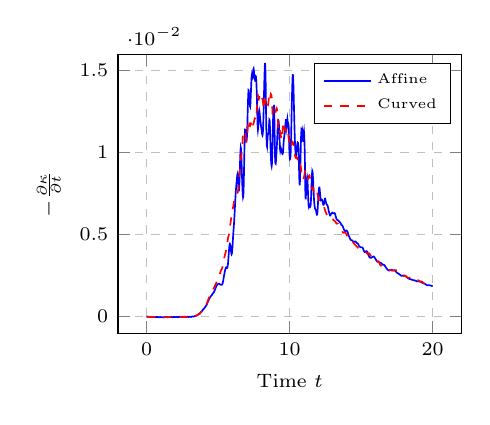
\begin{tikzpicture}
\begin{axis}[
    width=.49\textwidth,
    xlabel={Time $t$},
    ylabel={$-\pd{\kappa}{t}$}, 
%    xmin=.0125, xmax=.75,
    ymin=-.001, ymax=.016,
    legend pos=north east, legend cell align=left, legend style={font=\tiny},	
    xmajorgrids=true, ymajorgrids=true, grid style=dashed,
    legend entries={Affine, Curved}    
]
\pgfplotsset{
cycle list={{blue}, {red, dashed}}
}

\addplot+[semithick, mark options={solid, fill=markercolor}]
coordinates{(0,-0)(0.02,-0)(0.04,-1e-06)(0.06,-2e-06)(0.08,-1e-06)(0.1,-0)(0.12,-0)(0.14,-2e-06)(0.16,-5e-06)(0.18,-8e-06)(0.2,-1.1e-05)(0.22,-1.3e-05)(0.24,-1.5e-05)(0.26,-1.5e-05)(0.28,-1.3e-05)(0.3,-1e-05)(0.32,-8e-06)(0.34,-8e-06)(0.36,-9e-06)(0.38,-1.1e-05)(0.4,-1.4e-05)(0.42,-1.7e-05)(0.44,-2e-05)(0.46,-2e-05)(0.48,-1.8e-05)(0.5,-1.6e-05)(0.52,-1.6e-05)(0.54,-1.7e-05)(0.56,-1.9e-05)(0.58,-2.2e-05)(0.6,-2.5e-05)(0.62,-2.7e-05)(0.64,-2.7e-05)(0.66,-2.3e-05)(0.68,-1.9e-05)(0.7,-1.5e-05)(0.72,-1.4e-05)(0.74,-1.5e-05)(0.76,-1.8e-05)(0.78,-2.3e-05)(0.8,-2.8e-05)(0.82,-3.2e-05)(0.84,-3.3e-05)(0.86,-3.1e-05)(0.88,-2.7e-05)(0.9,-2.4e-05)(0.92,-2.2e-05)(0.94,-2e-05)(0.96,-2e-05)(0.98,-2.2e-05)(1,-2.6e-05)(1.02,-2.9e-05)(1.04,-2.9e-05)(1.06,-2.8e-05)(1.08,-2.6e-05)(1.1,-2.4e-05)(1.12,-2.2e-05)(1.14,-2.2e-05)(1.16,-2.4e-05)(1.18,-2.8e-05)(1.2,-3.2e-05)(1.22,-3.2e-05)(1.24,-3e-05)(1.26,-2.7e-05)(1.28,-2.4e-05)(1.3,-2.1e-05)(1.32,-2e-05)(1.34,-2e-05)(1.36,-2.2e-05)(1.38,-2.3e-05)(1.4,-2.5e-05)(1.42,-2.6e-05)(1.44,-2.6e-05)(1.46,-2.7e-05)(1.48,-2.7e-05)(1.5,-2.6e-05)(1.52,-2.5e-05)(1.54,-2.3e-05)(1.56,-2.1e-05)(1.58,-2.1e-05)(1.6,-2.1e-05)(1.62,-2.1e-05)(1.64,-2.2e-05)(1.66,-2.1e-05)(1.68,-2e-05)(1.7,-1.9e-05)(1.72,-1.8e-05)(1.74,-1.8e-05)(1.76,-2e-05)(1.78,-2.4e-05)(1.8,-2.6e-05)(1.82,-2.7e-05)(1.84,-2.4e-05)(1.86,-2e-05)(1.88,-1.5e-05)(1.9,-1.1e-05)(1.92,-1.1e-05)(1.94,-1.4e-05)(1.96,-1.9e-05)(1.98,-2.3e-05)(2,-2.5e-05)(2.02,-2.3e-05)(2.04,-1.8e-05)(2.06,-1.2e-05)(2.08,-8e-06)(2.1,-8e-06)(2.12,-1.2e-05)(2.14,-1.8e-05)(2.16,-2.4e-05)(2.18,-2.7e-05)(2.2,-2.5e-05)(2.22,-1.9e-05)(2.24,-1.1e-05)(2.26,-5e-06)(2.28,-2e-06)(2.3,-3e-06)(2.32,-8e-06)(2.34,-1.5e-05)(2.36,-2.2e-05)(2.38,-2.5e-05)(2.4,-2.3e-05)(2.42,-1.8e-05)(2.44,-1.2e-05)(2.46,-6e-06)(2.48,-3e-06)(2.5,-3e-06)(2.52,-8e-06)(2.54,-1.5e-05)(2.56,-1.9e-05)(2.58,-2e-05)(2.6,-1.6e-05)(2.62,-1.1e-05)(2.64,-6e-06)(2.66,-2e-06)(2.68,-1e-06)(2.7,-5e-06)(2.72,-1.2e-05)(2.74,-1.9e-05)(2.76,-2.1e-05)(2.78,-1.8e-05)(2.8,-1.2e-05)(2.82,-5e-06)(2.84,1e-06)(2.86,3e-06)(2.88,0)(2.9,-7e-06)(2.92,-1.4e-05)(2.94,-1.6e-05)(2.96,-1.3e-05)(2.98,-6e-06)(3,2e-06)(3.02,7e-06)(3.04,8e-06)(3.06,3e-06)(3.08,-4e-06)(3.1,-1.1e-05)(3.12,-1.2e-05)(3.14,-6e-06)(3.16,5e-06)(3.18,1.6e-05)(3.2,2.2e-05)(3.22,2.3e-05)(3.24,2e-05)(3.26,1.5e-05)(3.28,1.1e-05)(3.3,1.2e-05)(3.32,1.8e-05)(3.34,2.9e-05)(3.36,3.9e-05)(3.38,4.7e-05)(3.4,5.3e-05)(3.42,5.7e-05)(3.44,6.1e-05)(3.46,6.5e-05)(3.48,6.9e-05)(3.5,7.5e-05)(3.52,8.4e-05)(3.54,9.5e-05)(3.56,0.000108)(3.58,0.000123)(3.6,0.000137)(3.62,0.000151)(3.64,0.00016)(3.66,0.000167)(3.68,0.000175)(3.7,0.000188)(3.72,0.000207)(3.74,0.00023)(3.76,0.000254)(3.78,0.000276)(3.8,0.000293)(3.82,0.000307)(3.84,0.00032)(3.86,0.000335)(3.88,0.000356)(3.9,0.000382)(3.92,0.00041)(3.94,0.000434)(3.96,0.000454)(3.98,0.000471)(4,0.000488)(4.02,0.000506)(4.04,0.000527)(4.06,0.00055)(4.08,0.000576)(4.1,0.000602)(4.12,0.000627)(4.14,0.000652)(4.16,0.000678)(4.18,0.000709)(4.2,0.000743)(4.22,0.00078)(4.24,0.000818)(4.26,0.000859)(4.28,0.000902)(4.3,0.000945)(4.32,0.000985)(4.34,0.001023)(4.36,0.001058)(4.38,0.001092)(4.4,0.001123)(4.42,0.001152)(4.44,0.001183)(4.46,0.001212)(4.48,0.001239)(4.5,0.001262)(4.52,0.001281)(4.54,0.001301)(4.56,0.001326)(4.58,0.001354)(4.6,0.001382)(4.62,0.001409)(4.64,0.001432)(4.66,0.001451)(4.68,0.00147)(4.7,0.001492)(4.72,0.001521)(4.74,0.001559)(4.76,0.001603)(4.78,0.001651)(4.8,0.001698)(4.82,0.001746)(4.84,0.001792)(4.86,0.001836)(4.88,0.001873)(4.9,0.001904)(4.92,0.001928)(4.94,0.001948)(4.96,0.001965)(4.98,0.001981)(5,0.001996)(5.02,0.002011)(5.04,0.002019)(5.06,0.002018)(5.08,0.002007)(5.1,0.00199)(5.12,0.001975)(5.14,0.001965)(5.16,0.00196)(5.18,0.001957)(5.2,0.001953)(5.22,0.001946)(5.24,0.001939)(5.26,0.001939)(5.28,0.001956)(5.3,0.001996)(5.32,0.002061)(5.34,0.002145)(5.36,0.00224)(5.38,0.002341)(5.4,0.002443)(5.42,0.002543)(5.44,0.002638)(5.46,0.002726)(5.48,0.002809)(5.5,0.002885)(5.52,0.002949)(5.54,0.002996)(5.56,0.003018)(5.58,0.003014)(5.6,0.002992)(5.62,0.002973)(5.64,0.002982)(5.66,0.003043)(5.68,0.00317)(5.7,0.003359)(5.72,0.003591)(5.74,0.003839)(5.76,0.004073)(5.78,0.004266)(5.8,0.004396)(5.82,0.004441)(5.84,0.004401)(5.86,0.004294)(5.88,0.00415)(5.9,0.003999)(5.92,0.003873)(5.94,0.003811)(5.96,0.003847)(5.98,0.003993)(6,0.004232)(6.02,0.004527)(6.04,0.004833)(6.06,0.005103)(6.08,0.005334)(6.1,0.005569)(6.12,0.005837)(6.14,0.006136)(6.16,0.006463)(6.18,0.006803)(6.2,0.007136)(6.22,0.00744)(6.24,0.007702)(6.26,0.007926)(6.28,0.008125)(6.3,0.008313)(6.32,0.008495)(6.34,0.008648)(6.36,0.00871)(6.38,0.008605)(6.4,0.008321)(6.42,0.007965)(6.44,0.007715)(6.46,0.007709)(6.48,0.007986)(6.5,0.008491)(6.52,0.009104)(6.54,0.009684)(6.56,0.010117)(6.58,0.010317)(6.6,0.010234)(6.62,0.009882)(6.64,0.009345)(6.66,0.008749)(6.68,0.008205)(6.7,0.007768)(6.72,0.007448)(6.74,0.007279)(6.76,0.007351)(6.78,0.007768)(6.8,0.008528)(6.82,0.009469)(6.84,0.010375)(6.86,0.011063)(6.88,0.011398)(6.9,0.011387)(6.92,0.01123)(6.94,0.011075)(6.96,0.01089)(6.98,0.010733)(7,0.010765)(7.02,0.01106)(7.04,0.011626)(7.06,0.012321)(7.08,0.012964)(7.1,0.013498)(7.12,0.013808)(7.14,0.013787)(7.16,0.013581)(7.18,0.013369)(7.2,0.013109)(7.22,0.012843)(7.24,0.012799)(7.26,0.01303)(7.28,0.013428)(7.3,0.013887)(7.32,0.014317)(7.34,0.014632)(7.36,0.014756)(7.38,0.014686)(7.4,0.014579)(7.42,0.014635)(7.44,0.014862)(7.46,0.015073)(7.48,0.015116)(7.5,0.014986)(7.52,0.014736)(7.54,0.014511)(7.56,0.014461)(7.58,0.014532)(7.6,0.014612)(7.62,0.014665)(7.64,0.014642)(7.66,0.014475)(7.68,0.014125)(7.7,0.013612)(7.72,0.012984)(7.74,0.012235)(7.76,0.01157)(7.78,0.011386)(7.8,0.01153)(7.82,0.011749)(7.84,0.012047)(7.86,0.012372)(7.88,0.012527)(7.9,0.012431)(7.92,0.012218)(7.94,0.012038)(7.96,0.01189)(7.98,0.011736)(8,0.011595)(8.02,0.011484)(8.04,0.01137)(8.06,0.011233)(8.08,0.011115)(8.1,0.011065)(8.12,0.011145)(8.14,0.011418)(8.16,0.011912)(8.18,0.012598)(8.2,0.013376)(8.22,0.014119)(8.24,0.014773)(8.26,0.01528)(8.28,0.015472)(8.3,0.015214)(8.32,0.014377)(8.34,0.013059)(8.36,0.01173)(8.38,0.010901)(8.4,0.010437)(8.42,0.01036)(8.44,0.010646)(8.46,0.010979)(8.48,0.011134)(8.5,0.011135)(8.52,0.011176)(8.54,0.011402)(8.56,0.011752)(8.58,0.012005)(8.6,0.011974)(8.62,0.011609)(8.64,0.011016)(8.66,0.010389)(8.68,0.009869)(8.7,0.009497)(8.72,0.009264)(8.74,0.009179)(8.76,0.00931)(8.78,0.009735)(8.8,0.010461)(8.82,0.011337)(8.84,0.012075)(8.86,0.012488)(8.88,0.01273)(8.9,0.012901)(8.92,0.012632)(8.94,0.011704)(8.96,0.010529)(8.98,0.009686)(9,0.009349)(9.02,0.009326)(9.04,0.009464)(9.06,0.009729)(9.08,0.010032)(9.1,0.010342)(9.12,0.010679)(9.14,0.011074)(9.16,0.011527)(9.18,0.01185)(9.2,0.011981)(9.22,0.011963)(9.24,0.011825)(9.26,0.011552)(9.28,0.011139)(9.3,0.010649)(9.32,0.010249)(9.34,0.010109)(9.36,0.010196)(9.38,0.010281)(9.4,0.01023)(9.42,0.010108)(9.44,0.010037)(9.46,0.010002)(9.48,0.009945)(9.5,0.009917)(9.52,0.009937)(9.54,0.01007)(9.56,0.010359)(9.58,0.010654)(9.6,0.010845)(9.62,0.010977)(9.64,0.011131)(9.66,0.011326)(9.68,0.011527)(9.7,0.011704)(9.72,0.011897)(9.74,0.012042)(9.76,0.01182)(9.78,0.011497)(9.8,0.011604)(9.82,0.011925)(9.84,0.012054)(9.86,0.011902)(9.88,0.011722)(9.9,0.01176)(9.92,0.011688)(9.94,0.011222)(9.96,0.010615)(9.98,0.010046)(10,0.009708)(10.02,0.009592)(10.04,0.009614)(10.06,0.0098)(10.08,0.010226)(10.1,0.01091)(10.12,0.011762)(10.14,0.012632)(10.16,0.013402)(10.18,0.014051)(10.2,0.014566)(10.22,0.014773)(10.24,0.014611)(10.26,0.014166)(10.28,0.013528)(10.3,0.012797)(10.32,0.012079)(10.34,0.01142)(10.36,0.010847)(10.38,0.010396)(10.4,0.010075)(10.42,0.009875)(10.44,0.009809)(10.46,0.009902)(10.48,0.010097)(10.5,0.010291)(10.52,0.010446)(10.54,0.01056)(10.56,0.010619)(10.58,0.010602)(10.6,0.010464)(10.62,0.010122)(10.64,0.009546)(10.66,0.008828)(10.68,0.00822)(10.7,0.008002)(10.72,0.008277)(10.74,0.008912)(10.76,0.009681)(10.78,0.010442)(10.8,0.011071)(10.82,0.011359)(10.84,0.011321)(10.86,0.011296)(10.88,0.011403)(10.9,0.011317)(10.92,0.010943)(10.94,0.010665)(10.96,0.010806)(10.98,0.011148)(11,0.01127)(11.02,0.011025)(11.04,0.010503)(11.06,0.009812)(11.08,0.00844)(11.1,0.007333)(11.12,0.00716)(11.14,0.007428)(11.16,0.007757)(11.18,0.008093)(11.2,0.008383)(11.22,0.008495)(11.24,0.008377)(11.26,0.008048)(11.28,0.007577)(11.3,0.007108)(11.32,0.006797)(11.34,0.006703)(11.36,0.006759)(11.38,0.00683)(11.4,0.006833)(11.42,0.006775)(11.44,0.00672)(11.46,0.006754)(11.48,0.006958)(11.5,0.007347)(11.52,0.007844)(11.54,0.008334)(11.56,0.008709)(11.58,0.008896)(11.6,0.008851)(11.62,0.008624)(11.64,0.0083)(11.66,0.007893)(11.68,0.007493)(11.7,0.007164)(11.72,0.006927)(11.74,0.006763)(11.76,0.006643)(11.78,0.006571)(11.8,0.006539)(11.82,0.006512)(11.84,0.006463)(11.86,0.006386)(11.88,0.006291)(11.9,0.006217)(11.92,0.006222)(11.94,0.006345)(11.96,0.006593)(11.98,0.006922)(12,0.007269)(12.02,0.007568)(12.04,0.007771)(12.06,0.007867)(12.08,0.007873)(12.1,0.007762)(12.12,0.007555)(12.14,0.007355)(12.16,0.007185)(12.18,0.007101)(12.2,0.007112)(12.22,0.007139)(12.24,0.007146)(12.26,0.007131)(12.28,0.007078)(12.3,0.006993)(12.32,0.00691)(12.34,0.006855)(12.36,0.006819)(12.38,0.006825)(12.4,0.006894)(12.42,0.007001)(12.44,0.007116)(12.46,0.007196)(12.48,0.007199)(12.5,0.007131)(12.52,0.007041)(12.54,0.00696)(12.56,0.006897)(12.58,0.006861)(12.6,0.006834)(12.62,0.00681)(12.64,0.006783)(12.66,0.006736)(12.68,0.006668)(12.7,0.006582)(12.72,0.006488)(12.74,0.006406)(12.76,0.00634)(12.78,0.006278)(12.8,0.006213)(12.82,0.006165)(12.84,0.006164)(12.86,0.006201)(12.88,0.006247)(12.9,0.006271)(12.92,0.006281)(12.94,0.0063)(12.96,0.006331)(12.98,0.006345)(13,0.006334)(13.02,0.006316)(13.04,0.006303)(13.06,0.006297)(13.08,0.006299)(13.1,0.006311)(13.12,0.006319)(13.14,0.006317)(13.16,0.006296)(13.18,0.006245)(13.2,0.006177)(13.22,0.006111)(13.24,0.006052)(13.26,0.005995)(13.28,0.005946)(13.3,0.005916)(13.32,0.005906)(13.34,0.0059)(13.36,0.005889)(13.38,0.005874)(13.4,0.005855)(13.42,0.005836)(13.44,0.005821)(13.46,0.005804)(13.48,0.005784)(13.5,0.005765)(13.52,0.005748)(13.54,0.005726)(13.56,0.005707)(13.58,0.005675)(13.6,0.00562)(13.62,0.005591)(13.64,0.005579)(13.66,0.005573)(13.68,0.00556)(13.7,0.00553)(13.72,0.005485)(13.74,0.005437)(13.76,0.005391)(13.78,0.005346)(13.8,0.005305)(13.82,0.00527)(13.84,0.005242)(13.86,0.005223)(13.88,0.005218)(13.9,0.005224)(13.92,0.005237)(13.94,0.00525)(13.96,0.005256)(13.98,0.005251)(14,0.005236)(14.02,0.005214)(14.04,0.005181)(14.06,0.005133)(14.08,0.005074)(14.1,0.005016)(14.12,0.004962)(14.14,0.004918)(14.16,0.004881)(14.18,0.004843)(14.2,0.004804)(14.22,0.004764)(14.24,0.004727)(14.26,0.004696)(14.28,0.004675)(14.3,0.004665)(14.32,0.004663)(14.34,0.004661)(14.36,0.004655)(14.38,0.004644)(14.4,0.004626)(14.42,0.004606)(14.44,0.004589)(14.46,0.004577)(14.48,0.00457)(14.5,0.004566)(14.52,0.00457)(14.54,0.004578)(14.56,0.004585)(14.58,0.004589)(14.6,0.004585)(14.62,0.004569)(14.64,0.004545)(14.66,0.004519)(14.68,0.004498)(14.7,0.004486)(14.72,0.004479)(14.74,0.004472)(14.76,0.00446)(14.78,0.004439)(14.8,0.004406)(14.82,0.004366)(14.84,0.004326)(14.86,0.004295)(14.88,0.004274)(14.9,0.004262)(14.92,0.004253)(14.94,0.004243)(14.96,0.004236)(14.98,0.004231)(15,0.004229)(15.02,0.004229)(15.04,0.004229)(15.06,0.004228)(15.08,0.004224)(15.1,0.004209)(15.12,0.004177)(15.14,0.004134)(15.16,0.004084)(15.18,0.004035)(15.2,0.003992)(15.22,0.003961)(15.24,0.003942)(15.26,0.003937)(15.28,0.003942)(15.3,0.003955)(15.32,0.003972)(15.34,0.003988)(15.36,0.003998)(15.38,0.004001)(15.4,0.003988)(15.42,0.003954)(15.44,0.003908)(15.46,0.003863)(15.48,0.003819)(15.5,0.003774)(15.52,0.003733)(15.54,0.003696)(15.56,0.00366)(15.58,0.00363)(15.6,0.003607)(15.62,0.003594)(15.64,0.003588)(15.66,0.003588)(15.68,0.003592)(15.7,0.003599)(15.72,0.003607)(15.74,0.003618)(15.76,0.003629)(15.78,0.003637)(15.8,0.003646)(15.82,0.003657)(15.84,0.003667)(15.86,0.003672)(15.88,0.003669)(15.9,0.003656)(15.92,0.003637)(15.94,0.003611)(15.96,0.003581)(15.98,0.00355)(16,0.00352)(16.02,0.00349)(16.04,0.003458)(16.06,0.003425)(16.08,0.003395)(16.1,0.003373)(16.12,0.003359)(16.14,0.003351)(16.16,0.003345)(16.18,0.003343)(16.2,0.003341)(16.22,0.003337)(16.24,0.00333)(16.26,0.003321)(16.28,0.003311)(16.3,0.003304)(16.32,0.003299)(16.34,0.003293)(16.36,0.003287)(16.38,0.003277)(16.4,0.003266)(16.42,0.003253)(16.44,0.003234)(16.46,0.003213)(16.48,0.003194)(16.5,0.003182)(16.52,0.003173)(16.54,0.003168)(16.56,0.003166)(16.58,0.003164)(16.6,0.003158)(16.62,0.003145)(16.64,0.003125)(16.66,0.003099)(16.68,0.003069)(16.7,0.003038)(16.72,0.003009)(16.74,0.002984)(16.76,0.002961)(16.78,0.002938)(16.8,0.002917)(16.82,0.002895)(16.84,0.002874)(16.86,0.002856)(16.88,0.002842)(16.9,0.002831)(16.92,0.002822)(16.94,0.002817)(16.96,0.002816)(16.98,0.002821)(17,0.00283)(17.02,0.00284)(17.04,0.002851)(17.06,0.002861)(17.08,0.002868)(17.1,0.00287)(17.12,0.002867)(17.14,0.00286)(17.16,0.002848)(17.18,0.002836)(17.2,0.002828)(17.22,0.002824)(17.24,0.002822)(17.26,0.002825)(17.28,0.002831)(17.3,0.002835)(17.32,0.002836)(17.34,0.00283)(17.36,0.002817)(17.38,0.002798)(17.4,0.002776)(17.42,0.002754)(17.44,0.002733)(17.46,0.002714)(17.48,0.002698)(17.5,0.002685)(17.52,0.002674)(17.54,0.002664)(17.56,0.002652)(17.58,0.002641)(17.6,0.002629)(17.62,0.002617)(17.64,0.002607)(17.66,0.002597)(17.68,0.002584)(17.7,0.002569)(17.72,0.002553)(17.74,0.002539)(17.76,0.002525)(17.78,0.002513)(17.8,0.002503)(17.82,0.002498)(17.84,0.002499)(17.86,0.002501)(17.88,0.002505)(17.9,0.002508)(17.92,0.002512)(17.94,0.002511)(17.96,0.002509)(17.98,0.002508)(18,0.002508)(18.02,0.002507)(18.04,0.002505)(18.06,0.002496)(18.08,0.002483)(18.1,0.002469)(18.12,0.002455)(18.14,0.002442)(18.16,0.002428)(18.18,0.002412)(18.2,0.002398)(18.22,0.002387)(18.24,0.002375)(18.26,0.002362)(18.28,0.00235)(18.3,0.002341)(18.32,0.002331)(18.34,0.002319)(18.36,0.002308)(18.38,0.0023)(18.4,0.002297)(18.42,0.002293)(18.44,0.002287)(18.46,0.002283)(18.48,0.002279)(18.5,0.002274)(18.52,0.002266)(18.54,0.002258)(18.56,0.00225)(18.58,0.002244)(18.6,0.00224)(18.62,0.002236)(18.64,0.002231)(18.66,0.002228)(18.68,0.002225)(18.7,0.002222)(18.72,0.002216)(18.74,0.002211)(18.76,0.002208)(18.78,0.002206)(18.8,0.002203)(18.82,0.002194)(18.84,0.002181)(18.86,0.002168)(18.88,0.002159)(18.9,0.002154)(18.92,0.002153)(18.94,0.002155)(18.96,0.002157)(18.98,0.002158)(19,0.002158)(19.02,0.002156)(19.04,0.002153)(19.06,0.00215)(19.08,0.002146)(19.1,0.002141)(19.12,0.002135)(19.14,0.002129)(19.16,0.002123)(19.18,0.002115)(19.2,0.002105)(19.22,0.002094)(19.24,0.002085)(19.26,0.002078)(19.28,0.00207)(19.3,0.002063)(19.32,0.002058)(19.34,0.002052)(19.36,0.002046)(19.38,0.002039)(19.4,0.002031)(19.42,0.002023)(19.44,0.002014)(19.46,0.002004)(19.48,0.001992)(19.5,0.001978)(19.52,0.001963)(19.54,0.001951)(19.56,0.00194)(19.58,0.001931)(19.6,0.001924)(19.62,0.00192)(19.64,0.001919)(19.66,0.001919)(19.68,0.001919)(19.7,0.001921)(19.72,0.001925)(19.74,0.001928)(19.76,0.001928)(19.78,0.001925)(19.8,0.001919)(19.82,0.001912)(19.84,0.001905)(19.86,0.001898)(19.88,0.001892)(19.9,0.001886)(19.92,0.001881)(19.94,0.001877)(19.96,0.001873)(19.98,0.001867)(20,0.001861)};

%coordinates{(0,-0)(0.1,-0)(0.2,-1.1e-05)(0.3,-1e-05)(0.4,-1.4e-05)(0.5,-1.6e-05)(0.6,-2.5e-05)(0.7,-1.5e-05)(0.8,-2.8e-05)(0.9,-2.4e-05)(1,-2.6e-05)(1.1,-2.4e-05)(1.2,-3.2e-05)(1.3,-2.1e-05)(1.4,-2.5e-05)(1.5,-2.6e-05)(1.6,-2.1e-05)(1.7,-1.9e-05)(1.8,-2.6e-05)(1.9,-1.1e-05)(2,-2.5e-05)(2.1,-8e-06)(2.2,-2.5e-05)(2.3,-3e-06)(2.4,-2.3e-05)(2.5,-3e-06)(2.6,-1.7e-05)(2.7,-5e-06)(2.8,-1.2e-05)(2.9,-8e-06)(3,1e-06)(3.1,-1.4e-05)(3.2,1.7e-05)(3.3,2e-06)(3.4,3.8e-05)(3.5,5.3e-05)(3.6,0.000105)(3.7,0.000139)(3.8,0.000221)(3.9,0.000276)(4,0.000342)(4.1,0.000419)(4.2,0.000521)(4.3,0.000678)(4.4,0.000837)(4.5,0.000981)(4.6,0.001062)(4.7,0.001087)(4.8,0.00113)(4.9,0.001166)(5,0.001202)(5.1,0.001253)(5.2,0.001359)(5.3,0.001478)(5.4,0.001732)(5.5,0.002089)(5.6,0.002263)(5.7,0.002498)(5.8,0.002994)(5.9,0.003125)(6,0.003437)(6.1,0.004011)(6.2,0.004722)(6.3,0.005376)(6.4,0.006272)(6.5,0.007188)(6.6,0.00777)(6.7,0.007294)(6.8,0.008198)(6.9,0.009458)(7,0.009693)(7.1,0.011262)(7.2,0.010684)(7.3,0.011183)(7.4,0.012658)(7.5,0.013435)(7.6,0.012556)(7.7,0.012895)(7.8,0.012983)(7.9,0.011737)(8,0.011435)(8.1,0.01177)(8.2,0.011534)(8.3,0.011911)(8.4,0.011895)(8.5,0.011791)(8.6,0.011377)(8.7,0.009956)(8.8,0.010736)(8.9,0.011693)(9,0.009853)(9.1,0.009799)(9.2,0.009839)(9.3,0.010534)(9.4,0.010571)(9.5,0.009947)(9.6,0.010718)(9.7,0.011076)(9.8,0.01093)(9.9,0.011329)(10,0.011703)(10.1,0.01164)(10.2,0.012807)(10.3,0.012246)(10.4,0.010467)(10.5,0.010364)(10.6,0.010194)(10.7,0.008977)(10.8,0.009781)(10.9,0.010854)(11,0.010576)(11.1,0.009041)(11.2,0.008563)(11.3,0.007785)(11.4,0.007869)(11.5,0.008274)(11.6,0.008207)(11.7,0.007814)(11.8,0.007557)(11.9,0.00751)(12,0.0082)(12.1,0.007652)(12.2,0.007354)(12.3,0.007167)(12.4,0.007458)(12.5,0.007237)(12.6,0.007162)(12.7,0.006955)(12.8,0.006604)(12.9,0.006469)(13,0.006581)(13.1,0.006469)(13.2,0.00626)(13.3,0.006146)(13.4,0.006075)(13.5,0.00601)(13.6,0.005883)(13.7,0.005825)(13.8,0.005701)(13.9,0.005585)(14,0.005407)(14.1,0.005251)(14.2,0.005187)(14.3,0.005117)(14.4,0.005088)(14.5,0.00498)(14.6,0.004898)(14.7,0.004772)(14.8,0.004717)(14.9,0.004651)(15,0.004603)(15.1,0.004514)(15.2,0.004408)(15.3,0.004296)(15.4,0.004199)(15.5,0.004117)(15.6,0.004069)(15.7,0.003965)(15.8,0.003854)(15.9,0.003777)(16,0.003716)(16.1,0.003633)(16.2,0.003617)(16.3,0.003594)(16.4,0.003547)(16.5,0.003478)(16.6,0.003385)(16.7,0.003317)(16.8,0.003279)(16.9,0.003207)(17,0.003162)(17.1,0.003144)(17.2,0.003097)(17.3,0.00307)(17.4,0.003008)(17.5,0.002939)(17.6,0.00292)(17.7,0.002873)(17.8,0.002805)(17.9,0.002742)(18,0.00271)(18.1,0.00266)(18.2,0.002629)(18.3,0.002588)(18.4,0.002547)(18.5,0.002515)(18.6,0.002468)(18.7,0.002415)(18.8,0.002386)(18.9,0.002366)(19,0.002338)(19.1,0.002301)(19.2,0.002265)(19.3,0.002243)(19.4,0.002204)(19.5,0.002174)(19.6,0.002139)(19.7,0.002107)(19.8,0.002075)(19.9,0.002052)(20,0.00202)};

\addplot+[semithick, mark options={solid, fill=markercolor}]
coordinates{(0,-0)(0.0199601,-0)(0.0399202,-1e-06)(0.0598802,-2e-06)(0.0798403,-2e-06)(0.0998004,-0)(0.11976,-0)(0.139721,-2e-06)(0.159681,-5e-06)(0.179641,-8e-06)(0.199601,-1.1e-05)(0.219561,-1.3e-05)(0.239521,-1.5e-05)(0.259481,-1.6e-05)(0.279441,-1.4e-05)(0.299401,-1.1e-05)(0.319361,-8e-06)(0.339321,-8e-06)(0.359281,-9e-06)(0.379242,-1.1e-05)(0.399202,-1.4e-05)(0.419162,-1.7e-05)(0.439122,-2e-05)(0.459082,-2e-05)(0.479042,-1.9e-05)(0.499002,-1.7e-05)(0.518962,-1.6e-05)(0.538922,-1.7e-05)(0.558882,-1.9e-05)(0.578842,-2.2e-05)(0.598802,-2.6e-05)(0.618762,-2.8e-05)(0.638723,-2.8e-05)(0.658683,-2.5e-05)(0.678643,-2e-05)(0.698603,-1.7e-05)(0.718563,-1.6e-05)(0.738523,-1.6e-05)(0.758483,-1.9e-05)(0.778443,-2.4e-05)(0.798403,-3e-05)(0.818363,-3.4e-05)(0.838323,-3.5e-05)(0.858283,-3.3e-05)(0.878244,-2.9e-05)(0.898204,-2.6e-05)(0.918164,-2.4e-05)(0.938124,-2.2e-05)(0.958084,-2.1e-05)(0.978044,-2.4e-05)(0.998004,-2.7e-05)(1.01796,-3e-05)(1.03792,-3.1e-05)(1.05788,-3e-05)(1.07784,-2.8e-05)(1.0978,-2.6e-05)(1.11776,-2.4e-05)(1.13772,-2.4e-05)(1.15768,-2.6e-05)(1.17764,-3e-05)(1.1976,-3.3e-05)(1.21756,-3.4e-05)(1.23752,-3.2e-05)(1.25749,-2.9e-05)(1.27745,-2.6e-05)(1.29741,-2.3e-05)(1.31737,-2.2e-05)(1.33733,-2.2e-05)(1.35729,-2.3e-05)(1.37725,-2.5e-05)(1.39721,-2.6e-05)(1.41717,-2.7e-05)(1.43713,-2.8e-05)(1.45709,-2.8e-05)(1.47705,-2.8e-05)(1.49701,-2.8e-05)(1.51697,-2.6e-05)(1.53693,-2.4e-05)(1.55689,-2.3e-05)(1.57685,-2.2e-05)(1.59681,-2.2e-05)(1.61677,-2.2e-05)(1.63673,-2.2e-05)(1.65669,-2.2e-05)(1.67665,-2.1e-05)(1.69661,-1.9e-05)(1.71657,-1.8e-05)(1.73653,-1.8e-05)(1.75649,-2e-05)(1.77645,-2.3e-05)(1.79641,-2.6e-05)(1.81637,-2.6e-05)(1.83633,-2.4e-05)(1.85629,-2e-05)(1.87625,-1.5e-05)(1.89621,-1.1e-05)(1.91617,-1e-05)(1.93613,-1.2e-05)(1.95609,-1.6e-05)(1.97605,-2.1e-05)(1.99601,-2.4e-05)(2.01597,-2.2e-05)(2.03593,-1.7e-05)(2.05589,-1.1e-05)(2.07585,-7e-06)(2.09581,-5e-06)(2.11577,-8e-06)(2.13573,-1.4e-05)(2.15569,-2.1e-05)(2.17565,-2.4e-05)(2.19561,-2.3e-05)(2.21557,-1.7e-05)(2.23553,-1e-05)(2.25549,-3e-06)(2.27545,1e-06)(2.29541,1e-06)(2.31537,-3e-06)(2.33533,-1e-05)(2.35529,-1.6e-05)(2.37525,-2e-05)(2.39521,-2e-05)(2.41517,-1.6e-05)(2.43513,-9e-06)(2.45509,-3e-06)(2.47505,1e-06)(2.49501,2e-06)(2.51497,-2e-06)(2.53493,-8e-06)(2.55489,-1.4e-05)(2.57485,-1.5e-05)(2.59481,-1.2e-05)(2.61477,-7e-06)(2.63473,-1e-06)(2.65469,3e-06)(2.67465,5e-06)(2.69461,2e-06)(2.71457,-4e-06)(2.73453,-1.1e-05)(2.75449,-1.5e-05)(2.77445,-1.3e-05)(2.79441,-7e-06)(2.81437,0)(2.83433,7e-06)(2.85429,1e-05)(2.87425,9e-06)(2.89421,3e-06)(2.91417,-4e-06)(2.93413,-9e-06)(2.95409,-7e-06)(2.97405,-0)(2.99401,8e-06)(3.01397,1.5e-05)(3.03393,1.7e-05)(3.05389,1.4e-05)(3.07385,8e-06)(3.09381,0)(3.11377,-3e-06)(3.13373,1e-06)(3.15369,1.1e-05)(3.17365,2.2e-05)(3.19361,3.1e-05)(3.21357,3.4e-05)(3.23353,3.2e-05)(3.25349,2.7e-05)(3.27345,2.2e-05)(3.29341,2e-05)(3.31337,2.5e-05)(3.33333,3.4e-05)(3.35329,4.5e-05)(3.37325,5.4e-05)(3.39321,5.9e-05)(3.41317,6.4e-05)(3.43313,6.7e-05)(3.45309,7e-05)(3.47305,7.4e-05)(3.49301,7.8e-05)(3.51297,8.6e-05)(3.53293,9.5e-05)(3.55289,0.000107)(3.57285,0.00012)(3.59281,0.000133)(3.61277,0.000145)(3.63273,0.000155)(3.65269,0.00016)(3.67265,0.000165)(3.69261,0.000172)(3.71257,0.000186)(3.73253,0.000206)(3.7525,0.000228)(3.77246,0.000249)(3.79242,0.000267)(3.81238,0.000281)(3.83234,0.000292)(3.8523,0.000304)(3.87226,0.000321)(3.89222,0.000344)(3.91218,0.000371)(3.93214,0.000397)(3.9521,0.000419)(3.97206,0.000438)(3.99202,0.000456)(4.01198,0.000476)(4.03194,0.000499)(4.0519,0.000526)(4.07186,0.000557)(4.09182,0.000591)(4.11178,0.000625)(4.13174,0.000659)(4.1517,0.000693)(4.17166,0.00073)(4.19162,0.000771)(4.21158,0.000815)(4.23154,0.00086)(4.2515,0.000906)(4.27146,0.000954)(4.29142,0.001002)(4.31138,0.00105)(4.33134,0.001095)(4.3513,0.001138)(4.37126,0.001179)(4.39122,0.001219)(4.41118,0.001257)(4.43114,0.001296)(4.4511,0.001334)(4.47106,0.001372)(4.49102,0.001406)(4.51098,0.001435)(4.53094,0.001463)(4.5509,0.001494)(4.57086,0.00153)(4.59082,0.001569)(4.61078,0.001607)(4.63074,0.001644)(4.6507,0.001676)(4.67066,0.001706)(4.69062,0.001734)(4.71058,0.001765)(4.73054,0.001801)(4.7505,0.00184)(4.77046,0.00188)(4.79042,0.001918)(4.81038,0.001954)(4.83034,0.001992)(4.8503,0.002033)(4.87026,0.002076)(4.89022,0.002119)(4.91018,0.002159)(4.93014,0.002197)(4.9501,0.002232)(4.97006,0.002267)(4.99002,0.002306)(5.00998,0.00235)(5.02994,0.002397)(5.0499,0.002446)(5.06986,0.002492)(5.08982,0.002537)(5.10978,0.002584)(5.12974,0.002636)(5.1497,0.002693)(5.16966,0.002751)(5.18962,0.002802)(5.20958,0.002843)(5.22954,0.002876)(5.2495,0.002904)(5.26946,0.002939)(5.28942,0.00299)(5.30938,0.003061)(5.32934,0.003148)(5.3493,0.003245)(5.36926,0.003342)(5.38922,0.003433)(5.40918,0.003518)(5.42914,0.003596)(5.4491,0.003671)(5.46906,0.003744)(5.48902,0.003812)(5.50898,0.003874)(5.52894,0.003946)(5.5489,0.004029)(5.56886,0.00411)(5.58882,0.004192)(5.60878,0.004287)(5.62874,0.004405)(5.6487,0.004542)(5.66866,0.004679)(5.68862,0.004792)(5.70858,0.004871)(5.72854,0.004926)(5.7485,0.004983)(5.76846,0.005073)(5.78842,0.00521)(5.80838,0.005363)(5.82834,0.005491)(5.8483,0.005607)(5.86826,0.005737)(5.88822,0.005864)(5.90818,0.005972)(5.92814,0.00607)(5.9481,0.006177)(5.96806,0.006295)(5.98802,0.006413)(6.00798,0.006521)(6.02794,0.006612)(6.0479,0.006694)(6.06786,0.006786)(6.08782,0.006894)(6.10778,0.007008)(6.12774,0.007101)(6.1477,0.007152)(6.16766,0.007172)(6.18762,0.007191)(6.20758,0.007216)(6.22754,0.007238)(6.2475,0.007253)(6.26747,0.007275)(6.28743,0.007316)(6.30739,0.007364)(6.32735,0.007411)(6.34731,0.007471)(6.36727,0.00756)(6.38723,0.007678)(6.40719,0.007808)(6.42715,0.007932)(6.44711,0.008059)(6.46707,0.008226)(6.48703,0.008455)(6.50699,0.008733)(6.52695,0.009014)(6.54691,0.009261)(6.56687,0.009464)(6.58683,0.009619)(6.60679,0.009746)(6.62675,0.009886)(6.64671,0.010054)(6.66667,0.010231)(6.68663,0.010408)(6.70659,0.010661)(6.72655,0.010973)(6.74651,0.011103)(6.76647,0.011172)(6.78643,0.01126)(6.80639,0.011311)(6.82635,0.011331)(6.84631,0.011337)(6.86627,0.011308)(6.88623,0.011217)(6.90619,0.011086)(6.92615,0.010956)(6.94611,0.010822)(6.96607,0.010705)(6.98603,0.010689)(7.00599,0.010798)(7.02595,0.010995)(7.04591,0.011235)(7.06587,0.011469)(7.08583,0.011682)(7.10579,0.011886)(7.12575,0.012018)(7.14571,0.011997)(7.16567,0.011844)(7.18563,0.0117)(7.20559,0.011624)(7.22555,0.011613)(7.24551,0.011661)(7.26547,0.011736)(7.28543,0.011784)(7.30539,0.011775)(7.32535,0.011715)(7.34531,0.011626)(7.36527,0.011528)(7.38523,0.011455)(7.40519,0.011437)(7.42515,0.011492)(7.44511,0.011601)(7.46507,0.011721)(7.48503,0.01182)(7.50499,0.011897)(7.52495,0.011971)(7.54491,0.012047)(7.56487,0.012092)(7.58483,0.012083)(7.60479,0.012026)(7.62475,0.011969)(7.64471,0.011992)(7.66467,0.012141)(7.68463,0.012396)(7.70459,0.012705)(7.72455,0.01302)(7.74451,0.013287)(7.76447,0.013446)(7.78443,0.013486)(7.80439,0.01343)(7.82435,0.013322)(7.84431,0.01326)(7.86427,0.013299)(7.88423,0.013392)(7.90419,0.013474)(7.92415,0.013537)(7.94411,0.013593)(7.96407,0.01362)(7.98403,0.013589)(8.00399,0.013514)(8.02395,0.013423)(8.04391,0.013344)(8.06387,0.013306)(8.08383,0.013303)(8.10379,0.013281)(8.12375,0.013184)(8.14371,0.012992)(8.16367,0.012774)(8.18363,0.012635)(8.20359,0.01263)(8.22355,0.012749)(8.24351,0.012938)(8.26347,0.013106)(8.28343,0.013176)(8.30339,0.01312)(8.32335,0.012971)(8.34331,0.012822)(8.36327,0.01278)(8.38323,0.012867)(8.40319,0.012987)(8.42315,0.013036)(8.44311,0.012996)(8.46307,0.012924)(8.48303,0.012907)(8.50299,0.012989)(8.52295,0.013142)(8.54291,0.013301)(8.56287,0.013392)(8.58283,0.01335)(8.60279,0.01321)(8.62275,0.013128)(8.64271,0.013227)(8.66267,0.013442)(8.68263,0.013568)(8.70259,0.013543)(8.72255,0.013503)(8.74251,0.013375)(8.76248,0.013106)(8.78244,0.012738)(8.8024,0.012366)(8.82236,0.012168)(8.84232,0.012145)(8.86228,0.01216)(8.88224,0.012192)(8.9022,0.012258)(8.92216,0.012312)(8.94212,0.012334)(8.96208,0.012352)(8.98204,0.012384)(9.002,0.012425)(9.02196,0.012481)(9.04192,0.012562)(9.06188,0.012657)(9.08184,0.012724)(9.1018,0.012704)(9.12176,0.012568)(9.14172,0.012341)(9.16168,0.012065)(9.18164,0.01177)(9.2016,0.011481)(9.22156,0.011248)(9.24152,0.011131)(9.26148,0.011144)(9.28144,0.01123)(9.3014,0.0113)(9.32136,0.011313)(9.34132,0.011273)(9.36128,0.011183)(9.38124,0.011049)(9.4012,0.010906)(9.42116,0.010804)(9.44112,0.010771)(9.46108,0.010824)(9.48104,0.010974)(9.501,0.011212)(9.52096,0.011492)(9.54092,0.01174)(9.56088,0.011883)(9.58084,0.011894)(9.6008,0.011792)(9.62076,0.01163)(9.64072,0.011484)(9.66068,0.011411)(9.68064,0.011421)(9.7006,0.011454)(9.72056,0.011447)(9.74052,0.011379)(9.76048,0.01126)(9.78044,0.011128)(9.8004,0.01102)(9.82036,0.010973)(9.84032,0.011012)(9.86028,0.011103)(9.88024,0.011151)(9.9002,0.011101)(9.92016,0.010978)(9.94012,0.010823)(9.96008,0.010657)(9.98004,0.010505)(10,0.010386)(10.02,0.01031)(10.0399,0.010298)(10.0599,0.010353)(10.0798,0.010436)(10.0998,0.010489)(10.1198,0.010507)(10.1397,0.010528)(10.1597,0.010575)(10.1796,0.010634)(10.1996,0.010664)(10.2196,0.010647)(10.2395,0.010595)(10.2595,0.010516)(10.2794,0.010414)(10.2994,0.010296)(10.3194,0.010168)(10.3393,0.010032)(10.3593,0.0099)(10.3792,0.009793)(10.3992,0.009726)(10.4192,0.00969)(10.4391,0.009673)(10.4591,0.00967)(10.479,0.009683)(10.499,0.009703)(10.519,0.009704)(10.5389,0.009676)(10.5589,0.009618)(10.5788,0.009525)(10.5988,0.009401)(10.6188,0.009274)(10.6387,0.009191)(10.6587,0.00918)(10.6786,0.009225)(10.6986,0.009276)(10.7186,0.009298)(10.7385,0.009281)(10.7585,0.009228)(10.7784,0.009132)(10.7984,0.008988)(10.8184,0.00882)(10.8383,0.008653)(10.8583,0.008513)(10.8782,0.008413)(10.8982,0.008363)(10.9182,0.008365)(10.9381,0.008395)(10.9581,0.008424)(10.978,0.008449)(10.998,0.008493)(11.018,0.008578)(11.0379,0.008693)(11.0579,0.008803)(11.0778,0.008868)(11.0978,0.00886)(11.1178,0.008782)(11.1377,0.008664)(11.1577,0.008549)(11.1776,0.008457)(11.1976,0.008396)(11.2176,0.008371)(11.2375,0.008366)(11.2575,0.008369)(11.2774,0.008387)(11.2974,0.008431)(11.3174,0.008493)(11.3373,0.008553)(11.3573,0.008601)(11.3772,0.008616)(11.3972,0.008576)(11.4172,0.008478)(11.4371,0.008351)(11.4571,0.008217)(11.477,0.008087)(11.497,0.007972)(11.517,0.007883)(11.5369,0.007832)(11.5569,0.007823)(11.5768,0.007847)(11.5968,0.00788)(11.6168,0.007887)(11.6367,0.007849)(11.6567,0.007768)(11.6766,0.007667)(11.6966,0.007577)(11.7166,0.007519)(11.7365,0.007498)(11.7565,0.007511)(11.7764,0.007547)(11.7964,0.007591)(11.8164,0.007634)(11.8363,0.007675)(11.8563,0.007701)(11.8762,0.007699)(11.8962,0.007664)(11.9162,0.007603)(11.9361,0.007525)(11.9561,0.007444)(11.976,0.007367)(11.996,0.007292)(12.016,0.007222)(12.0359,0.007157)(12.0559,0.007101)(12.0758,0.007055)(12.0958,0.007014)(12.1158,0.006972)(12.1357,0.006937)(12.1557,0.006912)(12.1756,0.006899)(12.1956,0.006899)(12.2156,0.006905)(12.2355,0.006903)(12.2555,0.006885)(12.2754,0.006852)(12.2954,0.00681)(12.3154,0.006769)(12.3353,0.006739)(12.3553,0.00672)(12.3752,0.006703)(12.3952,0.006679)(12.4152,0.006647)(12.4351,0.006603)(12.4551,0.006548)(12.475,0.006487)(12.495,0.006428)(12.515,0.00638)(12.5349,0.006342)(12.5549,0.006308)(12.5749,0.00627)(12.5948,0.006229)(12.6148,0.006193)(12.6347,0.006169)(12.6547,0.006158)(12.6747,0.006159)(12.6946,0.006163)(12.7146,0.006169)(12.7345,0.006175)(12.7545,0.006173)(12.7745,0.006163)(12.7944,0.00615)(12.8144,0.006137)(12.8343,0.006122)(12.8543,0.006111)(12.8743,0.00611)(12.8942,0.006118)(12.9142,0.006126)(12.9341,0.006125)(12.9541,0.006106)(12.9741,0.00607)(12.994,0.006026)(13.014,0.005978)(13.0339,0.00593)(13.0539,0.005893)(13.0739,0.005875)(13.0938,0.005865)(13.1138,0.005852)(13.1337,0.005838)(13.1537,0.005827)(13.1737,0.005813)(13.1936,0.005793)(13.2136,0.005768)(13.2335,0.00574)(13.2535,0.005709)(13.2735,0.005681)(13.2934,0.00567)(13.3134,0.005675)(13.3333,0.005685)(13.3533,0.005687)(13.3733,0.005669)(13.3932,0.005632)(13.4132,0.005586)(13.4331,0.005539)(13.4531,0.005497)(13.4731,0.005466)(13.493,0.005442)(13.513,0.005417)(13.5329,0.005392)(13.5529,0.005369)(13.5729,0.005352)(13.5928,0.005334)(13.6128,0.005312)(13.6327,0.005288)(13.6527,0.005259)(13.6727,0.005223)(13.6926,0.005183)(13.7126,0.005147)(13.7325,0.005124)(13.7525,0.005114)(13.7725,0.005113)(13.7924,0.005121)(13.8124,0.005132)(13.8323,0.005141)(13.8523,0.005145)(13.8723,0.005142)(13.8922,0.005127)(13.9122,0.005103)(13.9321,0.005073)(13.9521,0.005042)(13.9721,0.005011)(13.992,0.004977)(14.012,0.004941)(14.0319,0.004907)(14.0519,0.004879)(14.0719,0.004861)(14.0918,0.004849)(14.1118,0.004838)(14.1317,0.004827)(14.1517,0.004815)(14.1717,0.004804)(14.1916,0.004792)(14.2116,0.004779)(14.2315,0.004768)(14.2515,0.004762)(14.2715,0.004759)(14.2914,0.004754)(14.3114,0.004743)(14.3313,0.004721)(14.3513,0.00469)(14.3713,0.004652)(14.3912,0.004613)(14.4112,0.004577)(14.4311,0.004544)(14.4511,0.004516)(14.4711,0.00449)(14.491,0.004465)(14.511,0.004443)(14.5309,0.004422)(14.5509,0.004403)(14.5709,0.004385)(14.5908,0.004368)(14.6108,0.004351)(14.6307,0.004333)(14.6507,0.004313)(14.6707,0.004293)(14.6906,0.004274)(14.7106,0.004257)(14.7305,0.004239)(14.7505,0.004221)(14.7705,0.004204)(14.7904,0.004192)(14.8104,0.004186)(14.8303,0.004183)(14.8503,0.00418)(14.8703,0.004175)(14.8902,0.004167)(14.9102,0.004152)(14.9301,0.004129)(14.9501,0.004104)(14.9701,0.004085)(14.99,0.004075)(15.01,0.00407)(15.0299,0.004067)(15.0499,0.004065)(15.0699,0.004062)(15.0898,0.004059)(15.1098,0.004053)(15.1297,0.004043)(15.1497,0.004028)(15.1697,0.004012)(15.1896,0.003996)(15.2096,0.003981)(15.2295,0.003971)(15.2495,0.003962)(15.2695,0.003955)(15.2894,0.003948)(15.3094,0.003938)(15.3293,0.003924)(15.3493,0.003908)(15.3693,0.003891)(15.3892,0.003872)(15.4092,0.003854)(15.4291,0.003842)(15.4491,0.00384)(15.4691,0.00385)(15.489,0.003863)(15.509,0.003872)(15.5289,0.003873)(15.5489,0.003866)(15.5689,0.003853)(15.5888,0.003833)(15.6088,0.003809)(15.6287,0.003778)(15.6487,0.003746)(15.6687,0.003715)(15.6886,0.003685)(15.7086,0.003655)(15.7285,0.003623)(15.7485,0.003591)(15.7685,0.003559)(15.7884,0.00353)(15.8084,0.003504)(15.8283,0.003479)(15.8483,0.003455)(15.8683,0.003431)(15.8882,0.003409)(15.9082,0.00339)(15.9281,0.003377)(15.9481,0.00337)(15.9681,0.003364)(15.988,0.003359)(16.008,0.003355)(16.0279,0.003353)(16.0479,0.003353)(16.0679,0.003356)(16.0878,0.003364)(16.1078,0.003375)(16.1277,0.003384)(16.1477,0.003389)(16.1677,0.003387)(16.1876,0.003381)(16.2076,0.003367)(16.2275,0.003346)(16.2475,0.003316)(16.2675,0.003276)(16.2874,0.003231)(16.3074,0.003188)(16.3273,0.003152)(16.3473,0.003128)(16.3673,0.003115)(16.3872,0.003112)(16.4072,0.003113)(16.4271,0.003115)(16.4471,0.003114)(16.4671,0.003111)(16.487,0.003106)(16.507,0.003097)(16.5269,0.003086)(16.5469,0.003074)(16.5669,0.003062)(16.5868,0.003051)(16.6068,0.003042)(16.6267,0.003036)(16.6467,0.003029)(16.6667,0.003021)(16.6866,0.003011)(16.7066,0.002998)(16.7265,0.002984)(16.7465,0.002968)(16.7665,0.002954)(16.7864,0.00294)(16.8064,0.002925)(16.8263,0.002905)(16.8463,0.002882)(16.8663,0.002858)(16.8862,0.00284)(16.9062,0.002829)(16.9261,0.002827)(16.9461,0.002829)(16.9661,0.002835)(16.986,0.002842)(17.006,0.002848)(17.0259,0.002849)(17.0459,0.002846)(17.0659,0.00284)(17.0858,0.002832)(17.1058,0.002822)(17.1257,0.002813)(17.1457,0.002808)(17.1657,0.002807)(17.1856,0.002808)(17.2056,0.00281)(17.2255,0.00281)(17.2455,0.002809)(17.2655,0.002808)(17.2854,0.002808)(17.3054,0.002808)(17.3253,0.00281)(17.3453,0.002815)(17.3653,0.002821)(17.3852,0.002825)(17.4052,0.002829)(17.4251,0.002832)(17.4451,0.002833)(17.4651,0.002833)(17.485,0.002832)(17.505,0.002827)(17.525,0.002819)(17.5449,0.002808)(17.5649,0.002792)(17.5848,0.00277)(17.6048,0.002741)(17.6248,0.002711)(17.6447,0.002681)(17.6647,0.002653)(17.6846,0.002629)(17.7046,0.002608)(17.7246,0.002591)(17.7445,0.002575)(17.7645,0.002559)(17.7844,0.002544)(17.8044,0.002533)(17.8244,0.002525)(17.8443,0.002518)(17.8643,0.002509)(17.8842,0.002498)(17.9042,0.002488)(17.9242,0.002483)(17.9441,0.002481)(17.9641,0.002484)(17.984,0.00249)(18.004,0.002499)(18.024,0.002507)(18.0439,0.00251)(18.0639,0.002507)(18.0838,0.002499)(18.1038,0.002488)(18.1238,0.002475)(18.1437,0.002459)(18.1637,0.002442)(18.1836,0.002424)(18.2036,0.002408)(18.2236,0.002394)(18.2435,0.002384)(18.2635,0.002376)(18.2834,0.002372)(18.3034,0.002369)(18.3234,0.002367)(18.3433,0.002367)(18.3633,0.00237)(18.3832,0.002374)(18.4032,0.002379)(18.4232,0.00238)(18.4431,0.002378)(18.4631,0.002373)(18.483,0.002365)(18.503,0.002354)(18.523,0.002343)(18.5429,0.00233)(18.5629,0.002317)(18.5828,0.002304)(18.6028,0.002291)(18.6228,0.002279)(18.6427,0.002268)(18.6627,0.002256)(18.6826,0.002243)(18.7026,0.002229)(18.7226,0.002213)(18.7425,0.002198)(18.7625,0.002187)(18.7824,0.002183)(18.8024,0.002182)(18.8224,0.002185)(18.8423,0.00219)(18.8623,0.002199)(18.8822,0.002208)(18.9022,0.002216)(18.9222,0.00222)(18.9421,0.002223)(18.9621,0.002224)(18.982,0.002221)(19.002,0.002214)(19.022,0.002203)(19.0419,0.002191)(19.0619,0.00218)(19.0818,0.00217)(19.1018,0.002163)(19.1218,0.002158)(19.1417,0.002155)(19.1617,0.002154)(19.1816,0.002152)(19.2016,0.002149)(19.2216,0.002145)(19.2415,0.002139)(19.2615,0.002129)(19.2814,0.002116)(19.3014,0.0021)(19.3214,0.002082)(19.3413,0.002065)(19.3613,0.002051)(19.3812,0.002037)(19.4012,0.002023)(19.4212,0.00201)(19.4411,0.001999)(19.4611,0.00199)(19.481,0.001983)(19.501,0.001978)(19.521,0.001976)(19.5409,0.001977)(19.5609,0.001979)(19.5808,0.001981)(19.6008,0.001985)(19.6208,0.001991)(19.6407,0.001998)(19.6607,0.002003)(19.6806,0.002005)(19.7006,0.002005)(19.7206,0.002004)(19.7405,0.002003)(19.7605,0.002001)(19.7804,0.001998)(19.8004,0.001993)(19.8204,0.001987)(19.8403,0.001979)(19.8603,0.00197)(19.8802,0.00196)(19.9002,0.00195)(19.9202,0.001941)(19.9401,0.001933)(19.9601,0.001925)(19.98,0.001917)(20,0.001908)};

%coordinates{(0,-0)(0.1,-0)(0.2,-1.1e-05)(0.3,-1e-05)(0.4,-1.3e-05)(0.5,-1.6e-05)(0.6,-2.5e-05)(0.7,-1.6e-05)(0.8,-2.8e-05)(0.9,-2.5e-05)(1,-2.5e-05)(1.1,-2.4e-05)(1.2,-3.1e-05)(1.3,-2.2e-05)(1.4,-2.4e-05)(1.5,-2.7e-05)(1.6,-2.1e-05)(1.7,-1.9e-05)(1.8,-2.6e-05)(1.9,-1.2e-05)(2,-2.5e-05)(2.1,-8e-06)(2.2,-2.6e-05)(2.3,-2e-06)(2.4,-2.4e-05)(2.5,-3e-06)(2.6,-1.8e-05)(2.7,-4e-06)(2.8,-1.5e-05)(2.9,-5e-06)(3,-3e-06)(3.1,-1.4e-05)(3.2,1.1e-05)(3.3,-5e-06)(3.4,2.5e-05)(3.5,3.2e-05)(3.6,7.1e-05)(3.7,9e-05)(3.8,0.000156)(3.9,0.000201)(4,0.000279)(4.1,0.000375)(4.2,0.00051)(4.3,0.000691)(4.4,0.000864)(4.5,0.001022)(4.6,0.00114)(4.7,0.001224)(4.8,0.001302)(4.9,0.001404)(5,0.001526)(5.1,0.001685)(5.2,0.001869)(5.3,0.002032)(5.4,0.002409)(5.5,0.002752)(5.6,0.003089)(5.7,0.003588)(5.8,0.004093)(5.9,0.004445)(6,0.004825)(6.1,0.005375)(6.2,0.005868)(6.3,0.006183)(6.4,0.006331)(6.5,0.006797)(6.6,0.007712)(6.7,0.008319)(6.8,0.00896)(6.9,0.009326)(7,0.009777)(7.1,0.010393)(7.2,0.010403)(7.3,0.010421)(7.4,0.010724)(7.5,0.011246)(7.6,0.011484)(7.7,0.011616)(7.8,0.012531)(7.9,0.012689)(8,0.012545)(8.1,0.012473)(8.2,0.012667)(8.3,0.012824)(8.4,0.012941)(8.5,0.0127)(8.6,0.012743)(8.7,0.012718)(8.8,0.012434)(8.9,0.011995)(9,0.011842)(9.1,0.01197)(9.2,0.011787)(9.3,0.011592)(9.4,0.011345)(9.5,0.010925)(9.6,0.011148)(9.7,0.01112)(9.8,0.010876)(9.9,0.010962)(10,0.010975)(10.1,0.010899)(10.2,0.010607)(10.3,0.010373)(10.4,0.01008)(10.5,0.009831)(10.6,0.009418)(10.7,0.009322)(10.8,0.009141)(10.9,0.009067)(11,0.009091)(11.1,0.008885)(11.2,0.008732)(11.3,0.008681)(11.4,0.008587)(11.5,0.008343)(11.6,0.008185)(11.7,0.008042)(11.8,0.008009)(11.9,0.007849)(12,0.007513)(12.1,0.007208)(12.2,0.007146)(12.3,0.007062)(12.4,0.007009)(12.5,0.006919)(12.6,0.006761)(12.7,0.006594)(12.8,0.006558)(12.9,0.00642)(13,0.00625)(13.1,0.006121)(13.2,0.006015)(13.3,0.00599)(13.4,0.00586)(13.5,0.005745)(13.6,0.005636)(13.7,0.005559)(13.8,0.005431)(13.9,0.005396)(14,0.005265)(14.1,0.0052)(14.2,0.005097)(14.3,0.004995)(14.4,0.004901)(14.5,0.004814)(14.6,0.0047)(14.7,0.004622)(14.8,0.004574)(14.9,0.004471)(15,0.004354)(15.1,0.004272)(15.2,0.00426)(15.3,0.004171)(15.4,0.004091)(15.5,0.004049)(15.6,0.003979)(15.7,0.003897)(15.8,0.003842)(15.9,0.003795)(16,0.003726)(16.1,0.003677)(16.2,0.003605)(16.3,0.003528)(16.4,0.003477)(16.5,0.003454)(16.6,0.003389)(16.7,0.003346)(16.8,0.003298)(16.9,0.003229)(17,0.003182)(17.1,0.003154)(17.2,0.003085)(17.3,0.003019)(17.4,0.002948)(17.5,0.002911)(17.6,0.002874)(17.7,0.002836)(17.8,0.002812)(17.9,0.002746)(18,0.0027)(18.1,0.002667)(18.2,0.002635)(18.3,0.002613)(18.4,0.002582)(18.5,0.002542)(18.6,0.002495)(18.7,0.002458)(18.8,0.002435)(18.9,0.002405)(19,0.002376)(19.1,0.002342)(19.2,0.002314)(19.3,0.002278)(19.4,0.00225)(19.5,0.00221)(19.6,0.002181)(19.7,0.002155)(19.8,0.002114)(19.9,0.002085)(20,0.002057)};

\end{axis}
\end{tikzpicture}
}
\subfloat[Gauss collocation]{
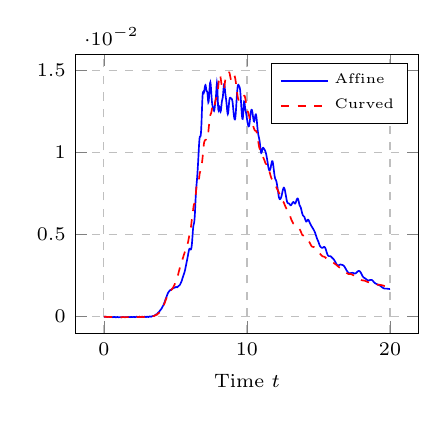
\begin{tikzpicture}
\begin{axis}[
    width=.49\textwidth,
    xlabel={Time $t$},
    ymin=-.001, ymax=.016,    
    legend pos=north east, legend cell align=left, legend style={font=\tiny},	
    xmajorgrids=true, ymajorgrids=true, grid style=dashed,
    legend entries={Affine, Curved}    
]
\pgfplotsset{
cycle list={{blue}, {red, dashed}}
}

\addplot+[semithick, mark options={solid, fill=markercolor}]
coordinates{(0,-0)(0.02,-0)(0.04,-1e-06)(0.06,-2e-06)(0.08,-1e-06)(0.1,-0)(0.12,-0)(0.14,-2e-06)(0.16,-5e-06)(0.18,-8e-06)(0.2,-1.1e-05)(0.22,-1.3e-05)(0.24,-1.5e-05)(0.26,-1.5e-05)(0.28,-1.3e-05)(0.3,-1e-05)(0.32,-8e-06)(0.34,-8e-06)(0.36,-9e-06)(0.38,-1.1e-05)(0.4,-1.4e-05)(0.42,-1.7e-05)(0.44,-2e-05)(0.46,-2e-05)(0.48,-1.8e-05)(0.5,-1.6e-05)(0.52,-1.6e-05)(0.54,-1.7e-05)(0.56,-1.9e-05)(0.58,-2.2e-05)(0.6,-2.5e-05)(0.62,-2.7e-05)(0.64,-2.7e-05)(0.66,-2.3e-05)(0.68,-1.9e-05)(0.7,-1.5e-05)(0.72,-1.4e-05)(0.74,-1.5e-05)(0.76,-1.8e-05)(0.78,-2.3e-05)(0.8,-2.8e-05)(0.82,-3.2e-05)(0.84,-3.3e-05)(0.86,-3.1e-05)(0.88,-2.7e-05)(0.9,-2.4e-05)(0.92,-2.2e-05)(0.94,-2e-05)(0.96,-2e-05)(0.98,-2.2e-05)(1,-2.6e-05)(1.02,-2.9e-05)(1.04,-2.9e-05)(1.06,-2.8e-05)(1.08,-2.6e-05)(1.1,-2.4e-05)(1.12,-2.2e-05)(1.14,-2.2e-05)(1.16,-2.4e-05)(1.18,-2.8e-05)(1.2,-3.2e-05)(1.22,-3.2e-05)(1.24,-3e-05)(1.26,-2.7e-05)(1.28,-2.4e-05)(1.3,-2.1e-05)(1.32,-2e-05)(1.34,-2e-05)(1.36,-2.2e-05)(1.38,-2.3e-05)(1.4,-2.5e-05)(1.42,-2.6e-05)(1.44,-2.6e-05)(1.46,-2.7e-05)(1.48,-2.7e-05)(1.5,-2.6e-05)(1.52,-2.5e-05)(1.54,-2.3e-05)(1.56,-2.1e-05)(1.58,-2.1e-05)(1.6,-2.1e-05)(1.62,-2.1e-05)(1.64,-2.2e-05)(1.66,-2.2e-05)(1.68,-2e-05)(1.7,-1.9e-05)(1.72,-1.8e-05)(1.74,-1.8e-05)(1.76,-2e-05)(1.78,-2.4e-05)(1.8,-2.6e-05)(1.82,-2.7e-05)(1.84,-2.4e-05)(1.86,-2e-05)(1.88,-1.5e-05)(1.9,-1.1e-05)(1.92,-1.1e-05)(1.94,-1.4e-05)(1.96,-1.9e-05)(1.98,-2.3e-05)(2,-2.5e-05)(2.02,-2.3e-05)(2.04,-1.8e-05)(2.06,-1.2e-05)(2.08,-8e-06)(2.1,-8e-06)(2.12,-1.2e-05)(2.14,-1.8e-05)(2.16,-2.4e-05)(2.18,-2.7e-05)(2.2,-2.5e-05)(2.22,-1.9e-05)(2.24,-1.1e-05)(2.26,-5e-06)(2.28,-2e-06)(2.3,-3e-06)(2.32,-8e-06)(2.34,-1.5e-05)(2.36,-2.2e-05)(2.38,-2.5e-05)(2.4,-2.3e-05)(2.42,-1.9e-05)(2.44,-1.2e-05)(2.46,-6e-06)(2.48,-3e-06)(2.5,-3e-06)(2.52,-8e-06)(2.54,-1.5e-05)(2.56,-2e-05)(2.58,-2e-05)(2.6,-1.7e-05)(2.62,-1.1e-05)(2.64,-6e-06)(2.66,-2e-06)(2.68,-1e-06)(2.7,-5e-06)(2.72,-1.2e-05)(2.74,-1.9e-05)(2.76,-2.1e-05)(2.78,-1.8e-05)(2.8,-1.2e-05)(2.82,-5e-06)(2.84,0)(2.86,2e-06)(2.88,-1e-06)(2.9,-8e-06)(2.92,-1.5e-05)(2.94,-1.8e-05)(2.96,-1.4e-05)(2.98,-7e-06)(3,0)(3.02,5e-06)(3.04,5e-06)(3.06,0)(3.08,-7e-06)(3.1,-1.4e-05)(3.12,-1.6e-05)(3.14,-1e-05)(3.16,0)(3.18,1e-05)(3.2,1.6e-05)(3.22,1.7e-05)(3.24,1.3e-05)(3.26,6e-06)(3.28,2e-06)(3.3,2e-06)(3.32,7e-06)(3.34,1.7e-05)(3.36,2.7e-05)(3.38,3.3e-05)(3.4,3.8e-05)(3.42,4.2e-05)(3.44,4.5e-05)(3.46,4.7e-05)(3.48,5e-05)(3.5,5.5e-05)(3.52,6.3e-05)(3.54,7.4e-05)(3.56,8.6e-05)(3.58,9.9e-05)(3.6,0.000113)(3.62,0.000125)(3.64,0.000134)(3.66,0.000139)(3.68,0.000145)(3.7,0.000157)(3.72,0.000175)(3.74,0.000197)(3.76,0.00022)(3.78,0.000241)(3.8,0.000259)(3.82,0.000272)(3.84,0.000284)(3.86,0.000299)(3.88,0.00032)(3.9,0.000347)(3.92,0.000375)(3.94,0.0004)(3.96,0.000422)(3.98,0.000442)(4,0.000462)(4.02,0.000485)(4.04,0.000511)(4.06,0.000542)(4.08,0.000576)(4.1,0.00061)(4.12,0.000644)(4.14,0.000678)(4.16,0.000713)(4.18,0.000752)(4.2,0.000794)(4.22,0.000839)(4.24,0.000885)(4.26,0.000932)(4.28,0.000983)(4.3,0.001034)(4.32,0.001084)(4.34,0.001132)(4.36,0.00118)(4.38,0.001227)(4.4,0.001274)(4.42,0.001319)(4.44,0.001365)(4.46,0.001409)(4.48,0.001448)(4.5,0.001479)(4.52,0.001504)(4.54,0.001526)(4.56,0.001548)(4.58,0.001572)(4.6,0.001593)(4.62,0.001611)(4.64,0.001625)(4.66,0.001633)(4.68,0.001639)(4.7,0.001646)(4.72,0.001656)(4.74,0.00167)(4.76,0.001686)(4.78,0.0017)(4.8,0.001711)(4.82,0.001721)(4.84,0.001732)(4.86,0.001743)(4.88,0.001754)(4.9,0.001762)(4.92,0.001769)(4.94,0.001774)(4.96,0.00178)(4.98,0.001787)(5,0.001796)(5.02,0.001806)(5.04,0.001812)(5.06,0.001811)(5.08,0.001805)(5.1,0.001797)(5.12,0.001795)(5.14,0.001804)(5.16,0.001821)(5.18,0.001842)(5.2,0.001863)(5.22,0.001878)(5.24,0.001888)(5.26,0.001896)(5.28,0.001909)(5.3,0.00193)(5.32,0.001959)(5.34,0.001994)(5.36,0.002029)(5.38,0.002065)(5.4,0.002103)(5.42,0.002146)(5.44,0.002194)(5.46,0.002248)(5.48,0.002305)(5.5,0.002362)(5.52,0.002418)(5.54,0.002471)(5.56,0.002521)(5.58,0.002571)(5.6,0.002622)(5.62,0.002677)(5.64,0.002736)(5.66,0.002803)(5.68,0.00288)(5.7,0.002965)(5.72,0.003054)(5.74,0.003142)(5.76,0.003228)(5.78,0.003314)(5.8,0.0034)(5.82,0.003489)(5.84,0.003578)(5.86,0.003669)(5.88,0.003764)(5.9,0.003864)(5.92,0.00396)(5.94,0.004043)(5.96,0.004104)(5.98,0.004138)(6,0.004146)(6.02,0.004134)(6.04,0.004113)(6.06,0.004097)(6.08,0.004101)(6.1,0.004136)(6.12,0.004212)(6.14,0.004337)(6.16,0.004517)(6.18,0.004744)(6.2,0.004996)(6.22,0.005239)(6.24,0.005437)(6.26,0.005568)(6.28,0.005643)(6.3,0.005703)(6.32,0.005804)(6.34,0.005992)(6.36,0.006275)(6.38,0.006628)(6.4,0.007004)(6.42,0.007354)(6.44,0.007652)(6.46,0.007894)(6.48,0.008101)(6.5,0.008301)(6.52,0.008515)(6.54,0.008758)(6.56,0.009031)(6.58,0.009332)(6.6,0.009652)(6.62,0.009985)(6.64,0.010314)(6.66,0.01061)(6.68,0.010831)(6.7,0.010951)(6.72,0.010982)(6.74,0.010981)(6.76,0.011019)(6.78,0.011153)(6.8,0.011407)(6.82,0.011781)(6.84,0.012246)(6.86,0.012745)(6.88,0.013194)(6.9,0.013516)(6.92,0.013678)(6.94,0.013701)(6.96,0.013658)(6.98,0.013635)(7,0.013684)(7.02,0.013795)(7.04,0.013922)(7.06,0.014027)(7.08,0.014096)(7.1,0.014113)(7.12,0.014057)(7.14,0.013939)(7.16,0.013814)(7.18,0.013747)(7.2,0.013742)(7.22,0.013726)(7.24,0.013619)(7.26,0.013414)(7.28,0.013189)(7.3,0.013059)(7.32,0.013094)(7.34,0.013284)(7.36,0.013556)(7.38,0.013834)(7.4,0.014071)(7.42,0.014236)(7.44,0.014291)(7.46,0.014208)(7.48,0.014001)(7.5,0.013728)(7.52,0.013455)(7.54,0.013221)(7.56,0.013039)(7.58,0.01291)(7.6,0.012821)(7.62,0.012753)(7.64,0.01269)(7.66,0.012624)(7.68,0.012564)(7.7,0.012544)(7.72,0.012597)(7.74,0.012718)(7.76,0.012866)(7.78,0.013005)(7.8,0.013137)(7.82,0.013294)(7.84,0.013512)(7.86,0.0138)(7.88,0.01409)(7.9,0.01424)(7.92,0.01413)(7.94,0.013761)(7.96,0.013269)(7.98,0.012841)(8,0.0126)(8.02,0.012558)(8.04,0.012636)(8.06,0.012737)(8.08,0.01279)(8.1,0.012763)(8.12,0.012669)(8.14,0.012562)(8.16,0.012513)(8.18,0.012566)(8.2,0.012715)(8.22,0.012905)(8.24,0.01307)(8.26,0.013178)(8.28,0.013247)(8.3,0.013327)(8.32,0.013459)(8.34,0.013653)(8.36,0.013873)(8.38,0.014057)(8.4,0.014155)(8.42,0.014146)(8.44,0.014037)(8.46,0.013864)(8.48,0.013677)(8.5,0.013513)(8.52,0.013375)(8.54,0.013243)(8.56,0.013093)(8.58,0.012915)(8.6,0.01272)(8.62,0.012536)(8.64,0.0124)(8.66,0.012347)(8.68,0.012392)(8.7,0.012531)(8.72,0.012731)(8.74,0.012946)(8.76,0.01313)(8.78,0.013257)(8.8,0.013325)(8.82,0.013349)(8.84,0.013347)(8.86,0.013332)(8.88,0.013315)(8.9,0.013302)(8.92,0.013291)(8.94,0.01327)(8.96,0.013227)(8.98,0.01315)(9,0.013029)(9.02,0.012865)(9.04,0.012673)(9.06,0.012479)(9.08,0.01231)(9.1,0.012178)(9.12,0.012083)(9.14,0.012027)(9.16,0.012022)(9.18,0.012085)(9.2,0.012225)(9.22,0.012436)(9.24,0.012698)(9.26,0.012986)(9.28,0.013276)(9.3,0.013543)(9.32,0.01377)(9.34,0.013946)(9.36,0.014065)(9.38,0.014125)(9.4,0.014134)(9.42,0.014107)(9.44,0.014066)(9.46,0.014029)(9.48,0.013994)(9.5,0.013937)(9.52,0.013831)(9.54,0.013661)(9.56,0.013431)(9.58,0.013164)(9.6,0.012882)(9.62,0.01261)(9.64,0.012366)(9.66,0.012174)(9.68,0.012061)(9.7,0.012053)(9.72,0.012173)(9.74,0.012411)(9.76,0.01271)(9.78,0.012975)(9.8,0.013117)(9.82,0.013106)(9.84,0.012978)(9.86,0.012812)(9.88,0.012668)(9.9,0.012565)(9.92,0.012487)(9.94,0.012405)(9.96,0.012305)(9.98,0.012186)(10,0.012059)(10.02,0.01194)(10.04,0.011836)(10.06,0.01175)(10.08,0.01168)(10.1,0.011629)(10.12,0.011603)(10.14,0.011615)(10.16,0.011675)(10.18,0.011786)(10.2,0.011937)(10.22,0.012107)(10.24,0.012272)(10.26,0.012413)(10.28,0.012518)(10.3,0.012583)(10.32,0.012611)(10.34,0.012604)(10.36,0.012561)(10.38,0.012474)(10.4,0.012349)(10.42,0.012211)(10.44,0.012083)(10.46,0.011978)(10.48,0.011908)(10.5,0.011896)(10.52,0.011949)(10.54,0.012046)(10.56,0.012154)(10.58,0.012246)(10.6,0.012309)(10.62,0.012327)(10.64,0.012289)(10.66,0.012188)(10.68,0.012031)(10.7,0.011838)(10.72,0.011638)(10.74,0.011454)(10.76,0.011297)(10.78,0.01117)(10.8,0.011069)(10.82,0.010986)(10.84,0.010909)(10.86,0.010824)(10.88,0.01072)(10.9,0.01059)(10.92,0.010438)(10.94,0.010275)(10.96,0.010126)(10.98,0.010022)(11,0.009978)(11.02,0.009995)(11.04,0.010053)(11.06,0.010128)(11.08,0.010201)(11.1,0.01026)(11.12,0.010294)(11.14,0.010299)(11.16,0.01028)(11.18,0.01025)(11.2,0.010219)(11.22,0.010192)(11.24,0.010165)(11.26,0.010134)(11.28,0.010096)(11.3,0.010047)(11.32,0.009986)(11.34,0.009912)(11.36,0.009829)(11.38,0.00974)(11.4,0.009645)(11.42,0.009542)(11.44,0.00943)(11.46,0.009313)(11.48,0.009197)(11.5,0.009094)(11.52,0.009012)(11.54,0.008957)(11.56,0.008928)(11.58,0.00892)(11.6,0.008931)(11.62,0.008964)(11.64,0.009019)(11.66,0.009094)(11.68,0.009183)(11.7,0.009278)(11.72,0.009369)(11.74,0.009442)(11.76,0.009484)(11.78,0.009484)(11.8,0.009438)(11.82,0.009348)(11.84,0.009224)(11.86,0.009082)(11.88,0.008935)(11.9,0.008792)(11.92,0.00866)(11.94,0.008548)(11.96,0.00846)(11.98,0.0084)(12,0.008361)(12.02,0.008332)(12.04,0.008297)(12.06,0.008241)(12.08,0.008161)(12.1,0.00806)(12.12,0.007947)(12.14,0.007827)(12.16,0.007702)(12.18,0.007577)(12.2,0.007456)(12.22,0.00735)(12.24,0.007266)(12.26,0.007208)(12.28,0.007175)(12.3,0.007163)(12.32,0.007167)(12.34,0.007184)(12.36,0.007213)(12.38,0.007253)(12.4,0.007304)(12.42,0.007368)(12.44,0.007442)(12.46,0.007522)(12.48,0.007604)(12.5,0.007684)(12.52,0.007756)(12.54,0.007814)(12.56,0.007851)(12.58,0.007864)(12.6,0.00785)(12.62,0.007813)(12.64,0.007753)(12.66,0.007675)(12.68,0.007585)(12.7,0.007487)(12.72,0.007387)(12.74,0.007285)(12.76,0.007187)(12.78,0.007099)(12.8,0.007027)(12.82,0.006974)(12.84,0.00694)(12.86,0.006921)(12.88,0.006913)(12.9,0.006911)(12.92,0.006907)(12.94,0.006897)(12.96,0.006881)(12.98,0.006859)(13,0.006836)(13.02,0.006813)(13.04,0.006797)(13.06,0.006792)(13.08,0.006801)(13.1,0.00682)(13.12,0.006846)(13.14,0.006875)(13.16,0.006904)(13.18,0.006934)(13.2,0.006961)(13.22,0.006981)(13.24,0.006991)(13.26,0.006988)(13.28,0.006973)(13.3,0.006948)(13.32,0.006921)(13.34,0.0069)(13.36,0.006894)(13.38,0.006905)(13.4,0.006935)(13.42,0.006978)(13.44,0.007031)(13.46,0.007087)(13.48,0.007138)(13.5,0.007177)(13.52,0.007201)(13.54,0.007207)(13.56,0.007192)(13.58,0.007154)(13.6,0.007091)(13.62,0.007012)(13.64,0.006928)(13.66,0.006852)(13.68,0.006794)(13.7,0.006754)(13.72,0.006725)(13.74,0.006695)(13.76,0.006654)(13.78,0.006597)(13.8,0.006527)(13.82,0.00645)(13.84,0.006373)(13.86,0.006304)(13.88,0.006246)(13.9,0.006203)(13.92,0.006172)(13.94,0.006151)(13.96,0.006134)(13.98,0.006117)(14,0.006094)(14.02,0.006063)(14.04,0.006021)(14.06,0.005971)(14.08,0.005916)(14.1,0.005863)(14.12,0.005822)(14.14,0.005799)(14.16,0.005797)(14.18,0.005813)(14.2,0.005841)(14.22,0.005873)(14.24,0.005901)(14.26,0.005916)(14.28,0.005914)(14.3,0.005897)(14.32,0.005867)(14.34,0.005829)(14.36,0.005787)(14.38,0.005746)(14.4,0.005707)(14.42,0.005672)(14.44,0.005639)(14.46,0.005607)(14.48,0.005574)(14.5,0.005541)(14.52,0.005509)(14.54,0.00548)(14.56,0.005451)(14.58,0.005423)(14.6,0.005396)(14.62,0.005369)(14.64,0.00534)(14.66,0.005309)(14.68,0.005275)(14.7,0.00524)(14.72,0.005204)(14.74,0.005166)(14.76,0.005124)(14.78,0.005077)(14.8,0.005027)(14.82,0.004972)(14.84,0.004914)(14.86,0.004857)(14.88,0.004804)(14.9,0.004758)(14.92,0.004717)(14.94,0.004678)(14.96,0.004638)(14.98,0.004597)(15,0.004552)(15.02,0.004504)(15.04,0.004453)(15.06,0.004403)(15.08,0.004359)(15.1,0.00432)(15.12,0.004289)(15.14,0.004263)(15.16,0.004245)(15.18,0.004231)(15.2,0.00422)(15.22,0.00421)(15.24,0.004201)(15.26,0.004197)(15.28,0.004199)(15.3,0.004206)(15.32,0.004217)(15.34,0.004231)(15.36,0.004245)(15.38,0.004255)(15.4,0.004258)(15.42,0.004251)(15.44,0.004235)(15.46,0.00421)(15.48,0.004176)(15.5,0.004133)(15.52,0.004082)(15.54,0.004025)(15.56,0.003966)(15.58,0.003908)(15.6,0.003853)(15.62,0.003805)(15.64,0.003768)(15.66,0.003739)(15.68,0.003719)(15.7,0.003705)(15.72,0.003696)(15.74,0.003693)(15.76,0.003693)(15.78,0.003694)(15.8,0.003694)(15.82,0.003692)(15.84,0.003687)(15.86,0.003677)(15.88,0.003662)(15.9,0.003643)(15.92,0.003624)(15.94,0.003606)(15.96,0.003589)(15.98,0.003572)(16,0.003556)(16.02,0.00354)(16.04,0.003522)(16.06,0.003502)(16.08,0.003479)(16.1,0.003453)(16.12,0.003426)(16.14,0.003397)(16.16,0.003366)(16.18,0.003333)(16.2,0.0033)(16.22,0.003268)(16.24,0.003237)(16.26,0.003208)(16.28,0.003181)(16.3,0.003159)(16.32,0.003142)(16.34,0.003131)(16.36,0.003124)(16.38,0.003123)(16.4,0.003127)(16.42,0.003136)(16.44,0.003147)(16.46,0.003157)(16.48,0.003166)(16.5,0.003174)(16.52,0.003178)(16.54,0.00318)(16.56,0.003178)(16.58,0.003175)(16.6,0.003172)(16.62,0.003168)(16.64,0.003165)(16.66,0.00316)(16.68,0.003155)(16.7,0.003148)(16.72,0.003139)(16.74,0.003125)(16.76,0.003109)(16.78,0.003091)(16.8,0.00307)(16.82,0.003046)(16.84,0.003019)(16.86,0.002989)(16.88,0.002959)(16.9,0.002928)(16.92,0.002896)(16.94,0.002865)(16.96,0.002835)(16.98,0.002808)(17,0.002781)(17.02,0.002756)(17.04,0.002733)(17.06,0.002712)(17.08,0.002694)(17.1,0.002679)(17.12,0.002666)(17.14,0.002656)(17.16,0.002651)(17.18,0.00265)(17.2,0.00265)(17.22,0.002652)(17.24,0.002656)(17.26,0.002661)(17.28,0.002667)(17.3,0.002671)(17.32,0.002673)(17.34,0.002675)(17.36,0.002677)(17.38,0.002676)(17.4,0.002673)(17.42,0.002668)(17.44,0.002664)(17.46,0.002659)(17.48,0.002652)(17.5,0.002645)(17.52,0.00264)(17.54,0.002637)(17.56,0.002638)(17.58,0.00264)(17.6,0.002647)(17.62,0.002658)(17.64,0.002672)(17.66,0.002689)(17.68,0.002707)(17.7,0.002725)(17.72,0.002743)(17.74,0.002759)(17.76,0.002772)(17.78,0.002782)(17.8,0.002788)(17.82,0.002791)(17.84,0.00279)(17.86,0.002783)(17.88,0.002772)(17.9,0.002756)(17.92,0.002736)(17.94,0.002712)(17.96,0.002682)(17.98,0.00265)(18,0.002615)(18.02,0.002579)(18.04,0.002544)(18.06,0.002509)(18.08,0.002478)(18.1,0.002451)(18.12,0.002429)(18.14,0.00241)(18.16,0.002395)(18.18,0.002382)(18.2,0.00237)(18.22,0.002359)(18.24,0.002348)(18.26,0.002336)(18.28,0.002323)(18.3,0.00231)(18.32,0.002298)(18.34,0.002285)(18.36,0.002272)(18.38,0.002259)(18.4,0.002248)(18.42,0.002237)(18.44,0.002228)(18.46,0.00222)(18.48,0.002216)(18.5,0.002214)(18.52,0.002215)(18.54,0.002219)(18.56,0.002223)(18.58,0.002229)(18.6,0.002236)(18.62,0.002241)(18.64,0.002245)(18.66,0.002247)(18.68,0.002248)(18.7,0.002247)(18.72,0.002242)(18.74,0.002233)(18.76,0.002221)(18.78,0.002206)(18.8,0.002188)(18.82,0.002168)(18.84,0.002146)(18.86,0.002125)(18.88,0.002106)(18.9,0.002089)(18.92,0.002072)(18.94,0.002057)(18.96,0.002044)(18.98,0.002033)(19,0.002023)(19.02,0.002013)(19.04,0.002003)(19.06,0.001996)(19.08,0.001989)(19.1,0.001982)(19.12,0.001974)(19.14,0.001966)(19.16,0.001958)(19.18,0.00195)(19.2,0.001941)(19.22,0.001932)(19.24,0.001923)(19.26,0.001916)(19.28,0.001908)(19.3,0.001897)(19.32,0.001885)(19.34,0.001873)(19.36,0.001859)(19.38,0.001844)(19.4,0.001828)(19.42,0.001813)(19.44,0.001799)(19.46,0.001786)(19.48,0.001774)(19.5,0.001762)(19.52,0.001752)(19.54,0.001743)(19.56,0.001735)(19.58,0.001727)(19.6,0.00172)(19.62,0.001716)(19.64,0.001714)(19.66,0.001713)(19.68,0.001713)(19.7,0.001714)(19.72,0.001715)(19.74,0.001715)(19.76,0.001714)(19.78,0.001711)(19.8,0.001709)(19.82,0.001707)(19.84,0.001704)(19.86,0.001702)(19.88,0.001699)(19.9,0.001697)(19.92,0.001696)(19.94,0.001694)(19.96,0.001692)(19.98,0.001691)(20,0.001692)};

\addplot+[semithick, mark options={solid, fill=markercolor}]
coordinates{(0,-0)(0.0199601,-0)(0.0399202,-1e-06)(0.0598802,-2e-06)(0.0798403,-1e-06)(0.0998004,-0)(0.11976,-0)(0.139721,-2e-06)(0.159681,-5e-06)(0.179641,-8e-06)(0.199601,-1.1e-05)(0.219561,-1.3e-05)(0.239521,-1.5e-05)(0.259481,-1.5e-05)(0.279441,-1.3e-05)(0.299401,-1e-05)(0.319361,-8e-06)(0.339321,-8e-06)(0.359281,-9e-06)(0.379242,-1.1e-05)(0.399202,-1.3e-05)(0.419162,-1.7e-05)(0.439122,-1.9e-05)(0.459082,-2e-05)(0.479042,-1.8e-05)(0.499002,-1.6e-05)(0.518962,-1.6e-05)(0.538922,-1.7e-05)(0.558882,-1.9e-05)(0.578842,-2.2e-05)(0.598802,-2.5e-05)(0.618762,-2.7e-05)(0.638723,-2.7e-05)(0.658683,-2.4e-05)(0.678643,-1.9e-05)(0.698603,-1.6e-05)(0.718563,-1.4e-05)(0.738523,-1.5e-05)(0.758483,-1.8e-05)(0.778443,-2.3e-05)(0.798403,-2.8e-05)(0.818363,-3.2e-05)(0.838323,-3.3e-05)(0.858283,-3.1e-05)(0.878244,-2.8e-05)(0.898204,-2.5e-05)(0.918164,-2.2e-05)(0.938124,-2e-05)(0.958084,-2e-05)(0.978044,-2.2e-05)(0.998004,-2.5e-05)(1.01796,-2.8e-05)(1.03792,-2.9e-05)(1.05788,-2.8e-05)(1.07784,-2.6e-05)(1.0978,-2.4e-05)(1.11776,-2.2e-05)(1.13772,-2.2e-05)(1.15768,-2.4e-05)(1.17764,-2.8e-05)(1.1976,-3.1e-05)(1.21756,-3.2e-05)(1.23752,-3e-05)(1.25749,-2.7e-05)(1.27745,-2.4e-05)(1.29741,-2.2e-05)(1.31737,-2e-05)(1.33733,-2e-05)(1.35729,-2.1e-05)(1.37725,-2.3e-05)(1.39721,-2.4e-05)(1.41717,-2.5e-05)(1.43713,-2.6e-05)(1.45709,-2.7e-05)(1.47705,-2.7e-05)(1.49701,-2.7e-05)(1.51697,-2.5e-05)(1.53693,-2.3e-05)(1.55689,-2.2e-05)(1.57685,-2.1e-05)(1.59681,-2.1e-05)(1.61677,-2.1e-05)(1.63673,-2.2e-05)(1.65669,-2.2e-05)(1.67665,-2.1e-05)(1.69661,-1.9e-05)(1.71657,-1.8e-05)(1.73653,-1.8e-05)(1.75649,-2e-05)(1.77645,-2.3e-05)(1.79641,-2.6e-05)(1.81637,-2.7e-05)(1.83633,-2.5e-05)(1.85629,-2.1e-05)(1.87625,-1.6e-05)(1.89621,-1.2e-05)(1.91617,-1.1e-05)(1.93613,-1.3e-05)(1.95609,-1.7e-05)(1.97605,-2.2e-05)(1.99601,-2.5e-05)(2.01597,-2.4e-05)(2.03593,-1.9e-05)(2.05589,-1.4e-05)(2.07585,-9e-06)(2.09581,-8e-06)(2.11577,-1.1e-05)(2.13573,-1.7e-05)(2.15569,-2.3e-05)(2.17565,-2.7e-05)(2.19561,-2.6e-05)(2.21557,-2.1e-05)(2.23553,-1.3e-05)(2.25549,-7e-06)(2.27545,-3e-06)(2.29541,-2e-06)(2.31537,-6e-06)(2.33533,-1.3e-05)(2.35529,-2e-05)(2.37525,-2.5e-05)(2.39521,-2.4e-05)(2.41517,-2e-05)(2.43513,-1.4e-05)(2.45509,-8e-06)(2.47505,-4e-06)(2.49501,-3e-06)(2.51497,-6e-06)(2.53493,-1.3e-05)(2.55489,-1.9e-05)(2.57485,-2e-05)(2.59481,-1.8e-05)(2.61477,-1.3e-05)(2.63473,-8e-06)(2.65469,-3e-06)(2.67465,-1e-06)(2.69461,-3e-06)(2.71457,-1e-05)(2.73453,-1.7e-05)(2.75449,-2.1e-05)(2.77445,-2e-05)(2.79441,-1.4e-05)(2.81437,-8e-06)(2.83433,-1e-06)(2.85429,2e-06)(2.87425,1e-06)(2.89421,-5e-06)(2.91417,-1.3e-05)(2.93413,-1.7e-05)(2.95409,-1.6e-05)(2.97405,-1e-05)(2.99401,-2e-06)(3.01397,4e-06)(3.03393,6e-06)(3.05389,3e-06)(3.07385,-5e-06)(3.09381,-1.3e-05)(3.11377,-1.7e-05)(3.13373,-1.4e-05)(3.15369,-5e-06)(3.17365,6e-06)(3.19361,1.3e-05)(3.21357,1.6e-05)(3.23353,1.3e-05)(3.25349,7e-06)(3.27345,1e-06)(3.29341,-2e-06)(3.31337,1e-06)(3.33333,9e-06)(3.35329,1.9e-05)(3.37325,2.6e-05)(3.39321,3.1e-05)(3.41317,3.4e-05)(3.43313,3.6e-05)(3.45309,3.8e-05)(3.47305,3.9e-05)(3.49301,4.2e-05)(3.51297,4.7e-05)(3.53293,5.5e-05)(3.55289,6.5e-05)(3.57285,7.5e-05)(3.59281,8.7e-05)(3.61277,9.8e-05)(3.63273,0.000105)(3.65269,0.000109)(3.67265,0.000111)(3.69261,0.000117)(3.71257,0.000129)(3.73253,0.000147)(3.7525,0.000167)(3.77246,0.000186)(3.79242,0.000203)(3.81238,0.000215)(3.83234,0.000225)(3.8523,0.000235)(3.87226,0.000251)(3.89222,0.000272)(3.91218,0.000297)(3.93214,0.000322)(3.9521,0.000344)(3.97206,0.000363)(3.99202,0.000381)(4.01198,0.000402)(4.03194,0.000426)(4.0519,0.000455)(4.07186,0.000489)(4.09182,0.000525)(4.11178,0.000562)(4.13174,0.000597)(4.1517,0.000633)(4.17166,0.000672)(4.19162,0.000714)(4.21158,0.000758)(4.23154,0.000803)(4.2515,0.00085)(4.27146,0.000898)(4.29142,0.000946)(4.31138,0.000994)(4.33134,0.001041)(4.3513,0.001086)(4.37126,0.00113)(4.39122,0.001174)(4.41118,0.001218)(4.43114,0.001262)(4.4511,0.001306)(4.47106,0.001348)(4.49102,0.001385)(4.51098,0.001415)(4.53094,0.001441)(4.5509,0.001468)(4.57086,0.001496)(4.59082,0.001526)(4.61078,0.001553)(4.63074,0.001576)(4.6507,0.001595)(4.67066,0.001609)(4.69062,0.001622)(4.71058,0.001636)(4.73054,0.001655)(4.7505,0.001677)(4.77046,0.001701)(4.79042,0.001724)(4.81038,0.001747)(4.83034,0.001773)(4.8503,0.001803)(4.87026,0.001837)(4.89022,0.001872)(4.91018,0.001908)(4.93014,0.001944)(4.9501,0.001982)(4.97006,0.002022)(4.99002,0.002067)(5.00998,0.002115)(5.02994,0.002165)(5.0499,0.002213)(5.06986,0.002256)(5.08982,0.002293)(5.10978,0.002333)(5.12974,0.002379)(5.1497,0.002436)(5.16966,0.002503)(5.18962,0.002575)(5.20958,0.002648)(5.22954,0.002719)(5.2495,0.002786)(5.26946,0.002853)(5.28942,0.002922)(5.30938,0.002996)(5.32934,0.003072)(5.3493,0.003144)(5.36926,0.003208)(5.38922,0.003262)(5.40918,0.003308)(5.42914,0.00335)(5.4491,0.003391)(5.46906,0.003435)(5.48902,0.003483)(5.50898,0.003537)(5.52894,0.003595)(5.5489,0.003654)(5.56886,0.003713)(5.58882,0.003769)(5.60878,0.003823)(5.62874,0.003875)(5.6487,0.003925)(5.66866,0.003971)(5.68862,0.004017)(5.70858,0.004065)(5.72854,0.004117)(5.7485,0.004171)(5.76846,0.004225)(5.78842,0.004277)(5.80838,0.004328)(5.82834,0.004379)(5.8483,0.004434)(5.86826,0.0045)(5.88822,0.004577)(5.90818,0.004665)(5.92814,0.004757)(5.9481,0.004848)(5.96806,0.004934)(5.98802,0.005016)(6.00798,0.005093)(6.02794,0.005172)(6.0479,0.00526)(6.06786,0.005365)(6.08782,0.005492)(6.10778,0.005635)(6.12774,0.005784)(6.1477,0.005932)(6.16766,0.006071)(6.18762,0.006201)(6.20758,0.006326)(6.22754,0.006455)(6.2475,0.00659)(6.26747,0.006717)(6.28743,0.006815)(6.30739,0.00687)(6.32735,0.006897)(6.34731,0.006931)(6.36727,0.007005)(6.38723,0.007136)(6.40719,0.007314)(6.42715,0.007512)(6.44711,0.007704)(6.46707,0.007871)(6.48703,0.008004)(6.50699,0.008101)(6.52695,0.008161)(6.54691,0.008183)(6.56687,0.008179)(6.58683,0.008172)(6.60679,0.008192)(6.62675,0.008262)(6.64671,0.008386)(6.66667,0.008536)(6.68663,0.008672)(6.70659,0.008769)(6.72655,0.008829)(6.74651,0.008873)(6.76647,0.008935)(6.78643,0.009029)(6.80639,0.00914)(6.82635,0.009241)(6.84631,0.009337)(6.86627,0.009453)(6.88623,0.009603)(6.90619,0.009778)(6.92615,0.009965)(6.94611,0.010158)(6.96607,0.010349)(6.98603,0.010511)(7.00599,0.010622)(7.02595,0.010685)(7.04591,0.010725)(7.06587,0.010754)(7.08583,0.010773)(7.10579,0.010782)(7.12575,0.010785)(7.14571,0.010784)(7.16567,0.010778)(7.18563,0.01077)(7.20559,0.01077)(7.22555,0.010792)(7.24551,0.010851)(7.26547,0.010956)(7.28543,0.011114)(7.30539,0.011307)(7.32535,0.011494)(7.34531,0.01165)(7.36527,0.011793)(7.38523,0.011948)(7.40519,0.012106)(7.42515,0.012233)(7.44511,0.012309)(7.46507,0.012349)(7.48503,0.012385)(7.50499,0.012442)(7.52495,0.01253)(7.54491,0.012631)(7.56487,0.012709)(7.58483,0.012737)(7.60479,0.012712)(7.62475,0.012656)(7.64471,0.012599)(7.66467,0.012577)(7.68463,0.012609)(7.70459,0.012691)(7.72455,0.012801)(7.74451,0.012921)(7.76447,0.013037)(7.78443,0.013135)(7.80439,0.013208)(7.82435,0.013259)(7.84431,0.013298)(7.86427,0.013341)(7.88423,0.0134)(7.90419,0.013479)(7.92415,0.013573)(7.94411,0.013679)(7.96407,0.013799)(7.98403,0.01394)(8.00399,0.014104)(8.02395,0.014284)(8.04391,0.014465)(8.06387,0.014621)(8.08383,0.014723)(8.10379,0.014756)(8.12375,0.014724)(8.14371,0.014644)(8.16367,0.014532)(8.18363,0.014402)(8.20359,0.014271)(8.22355,0.014154)(8.24351,0.014054)(8.26347,0.013965)(8.28343,0.01389)(8.30339,0.01384)(8.32335,0.013817)(8.34331,0.013811)(8.36327,0.013812)(8.38323,0.013833)(8.40319,0.013896)(8.42315,0.014009)(8.44311,0.014156)(8.46307,0.014306)(8.48303,0.014437)(8.50299,0.014541)(8.52295,0.014624)(8.54291,0.014687)(8.56287,0.014731)(8.58283,0.014767)(8.60279,0.014801)(8.62275,0.014831)(8.64271,0.014852)(8.66267,0.014863)(8.68263,0.014866)(8.70259,0.014867)(8.72255,0.014876)(8.74251,0.01489)(8.76248,0.014888)(8.78244,0.014848)(8.8024,0.014772)(8.82236,0.014676)(8.84232,0.014581)(8.86228,0.0145)(8.88224,0.014442)(8.9022,0.014418)(8.92216,0.014439)(8.94212,0.014507)(8.96208,0.014602)(8.98204,0.014686)(9.002,0.014731)(9.02196,0.014741)(9.04192,0.014739)(9.06188,0.014742)(9.08184,0.014743)(9.1018,0.014733)(9.12176,0.014704)(9.14172,0.014656)(9.16168,0.014592)(9.18164,0.014514)(9.2016,0.014415)(9.22156,0.014291)(9.24152,0.014146)(9.26148,0.013995)(9.28144,0.013853)(9.3014,0.013721)(9.32136,0.013596)(9.34132,0.013476)(9.36128,0.013367)(9.38124,0.013283)(9.4012,0.013234)(9.42116,0.013224)(9.44112,0.013246)(9.46108,0.013282)(9.48104,0.013316)(9.501,0.01334)(9.52096,0.013355)(9.54092,0.013368)(9.56088,0.013377)(9.58084,0.013374)(9.6008,0.013353)(9.62076,0.01332)(9.64072,0.013289)(9.66068,0.013272)(9.68064,0.013275)(9.7006,0.013292)(9.72056,0.013317)(9.74052,0.013352)(9.76048,0.013394)(9.78044,0.013436)(9.8004,0.013465)(9.82036,0.013468)(9.84032,0.013443)(9.86028,0.013393)(9.88024,0.013322)(9.9002,0.013233)(9.92016,0.013129)(9.94012,0.013014)(9.96008,0.012895)(9.98004,0.012779)(10,0.012676)(10.02,0.012594)(10.0399,0.012536)(10.0599,0.012495)(10.0798,0.01246)(10.0998,0.012416)(10.1198,0.012357)(10.1397,0.01228)(10.1597,0.012191)(10.1796,0.012098)(10.1996,0.012007)(10.2196,0.011929)(10.2395,0.011865)(10.2595,0.011817)(10.2794,0.011781)(10.2994,0.011755)(10.3194,0.011735)(10.3393,0.01172)(10.3593,0.011705)(10.3792,0.011687)(10.3992,0.011663)(10.4192,0.011633)(10.4391,0.011596)(10.4591,0.011553)(10.479,0.011505)(10.499,0.011455)(10.519,0.011409)(10.5389,0.011373)(10.5589,0.011347)(10.5788,0.011334)(10.5988,0.01133)(10.6188,0.011328)(10.6387,0.011317)(10.6587,0.011289)(10.6786,0.011239)(10.6986,0.011167)(10.7186,0.011078)(10.7385,0.010975)(10.7585,0.010863)(10.7784,0.010745)(10.7984,0.010626)(10.8184,0.010512)(10.8383,0.01041)(10.8583,0.010323)(10.8782,0.010255)(10.8982,0.010206)(10.9182,0.010173)(10.9381,0.010149)(10.9581,0.010129)(10.978,0.010106)(10.998,0.010078)(11.018,0.01004)(11.0379,0.009989)(11.0579,0.009928)(11.0778,0.009861)(11.0978,0.009799)(11.1178,0.009745)(11.1377,0.009701)(11.1577,0.009663)(11.1776,0.009627)(11.1976,0.009589)(11.2176,0.009545)(11.2375,0.009494)(11.2575,0.009441)(11.2774,0.009393)(11.2974,0.009353)(11.3174,0.009325)(11.3373,0.00931)(11.3573,0.009306)(11.3772,0.009309)(11.3972,0.009313)(11.4172,0.009307)(11.4371,0.009287)(11.4571,0.00925)(11.477,0.009199)(11.497,0.009135)(11.517,0.009063)(11.5369,0.008987)(11.5569,0.008912)(11.5768,0.00884)(11.5968,0.008771)(11.6168,0.008703)(11.6367,0.008638)(11.6567,0.008576)(11.6766,0.00852)(11.6966,0.008471)(11.7166,0.008429)(11.7365,0.008394)(11.7565,0.008364)(11.7764,0.008338)(11.7964,0.008311)(11.8164,0.008279)(11.8363,0.008244)(11.8563,0.008205)(11.8762,0.008167)(11.8962,0.008131)(11.9162,0.0081)(11.9361,0.008074)(11.9561,0.008051)(11.976,0.008026)(11.996,0.007996)(12.016,0.00796)(12.0359,0.007921)(12.0559,0.007882)(12.0758,0.007844)(12.0958,0.007806)(12.1158,0.00777)(12.1357,0.007735)(12.1557,0.007701)(12.1756,0.007667)(12.1956,0.007631)(12.2156,0.007593)(12.2355,0.007555)(12.2555,0.007515)(12.2754,0.007473)(12.2954,0.007428)(12.3154,0.00738)(12.3353,0.007331)(12.3553,0.007282)(12.3752,0.007233)(12.3952,0.007187)(12.4152,0.007147)(12.4351,0.007114)(12.4551,0.007087)(12.475,0.007066)(12.495,0.007048)(12.515,0.007032)(12.5349,0.007013)(12.5549,0.006988)(12.5749,0.006955)(12.5948,0.006916)(12.6148,0.006874)(12.6347,0.00683)(12.6547,0.006784)(12.6747,0.00674)(12.6946,0.006699)(12.7146,0.006662)(12.7345,0.006629)(12.7545,0.0066)(12.7745,0.006575)(12.7944,0.006553)(12.8144,0.006534)(12.8343,0.006514)(12.8543,0.006491)(12.8743,0.006464)(12.8942,0.006433)(12.9142,0.006397)(12.9341,0.006354)(12.9541,0.006306)(12.9741,0.006253)(12.994,0.006198)(13.014,0.006142)(13.0339,0.006087)(13.0539,0.006033)(13.0739,0.005983)(13.0938,0.005939)(13.1138,0.005898)(13.1337,0.005859)(13.1537,0.005821)(13.1737,0.005785)(13.1936,0.005751)(13.2136,0.005719)(13.2335,0.005691)(13.2535,0.005669)(13.2735,0.005656)(13.2934,0.005651)(13.3134,0.005649)(13.3333,0.005648)(13.3533,0.005647)(13.3733,0.005644)(13.3932,0.005638)(13.4132,0.005627)(13.4331,0.005612)(13.4531,0.005594)(13.4731,0.005576)(13.493,0.005556)(13.513,0.005536)(13.5329,0.005515)(13.5529,0.005492)(13.5729,0.005468)(13.5928,0.005442)(13.6128,0.005414)(13.6327,0.005387)(13.6527,0.005361)(13.6727,0.005338)(13.6926,0.005314)(13.7126,0.005287)(13.7325,0.005255)(13.7525,0.005219)(13.7725,0.005177)(13.7924,0.005132)(13.8124,0.005087)(13.8323,0.005046)(13.8523,0.005011)(13.8723,0.004984)(13.8922,0.004965)(13.9122,0.004955)(13.9321,0.004953)(13.9521,0.004956)(13.9721,0.004959)(13.992,0.004961)(14.012,0.004959)(14.0319,0.004952)(14.0519,0.00494)(14.0719,0.004922)(14.0918,0.004897)(14.1118,0.004869)(14.1317,0.004839)(14.1517,0.004807)(14.1717,0.004777)(14.1916,0.004749)(14.2116,0.004723)(14.2315,0.004699)(14.2515,0.004678)(14.2715,0.004656)(14.2914,0.004634)(14.3114,0.004612)(14.3313,0.004588)(14.3513,0.004561)(14.3713,0.004532)(14.3912,0.0045)(14.4112,0.004466)(14.4311,0.004431)(14.4511,0.004397)(14.4711,0.004364)(14.491,0.004334)(14.511,0.004309)(14.5309,0.004289)(14.5509,0.004275)(14.5709,0.004265)(14.5908,0.004258)(14.6108,0.004255)(14.6307,0.004254)(14.6507,0.004252)(14.6707,0.004247)(14.6906,0.004239)(14.7106,0.004229)(14.7305,0.004216)(14.7505,0.004199)(14.7705,0.004179)(14.7904,0.004156)(14.8104,0.004131)(14.8303,0.004104)(14.8503,0.004076)(14.8703,0.004047)(14.8902,0.004019)(14.9102,0.003995)(14.9301,0.003972)(14.9501,0.003952)(14.9701,0.003934)(14.99,0.00392)(15.01,0.003907)(15.0299,0.003894)(15.0499,0.003881)(15.0699,0.003867)(15.0898,0.003853)(15.1098,0.003837)(15.1297,0.003819)(15.1497,0.003799)(15.1697,0.003779)(15.1896,0.003759)(15.2096,0.003741)(15.2295,0.003722)(15.2495,0.003706)(15.2695,0.003693)(15.2894,0.003684)(15.3094,0.003676)(15.3293,0.003669)(15.3493,0.003665)(15.3693,0.003662)(15.3892,0.003658)(15.4092,0.003652)(15.4291,0.003644)(15.4491,0.003633)(15.4691,0.00362)(15.489,0.003605)(15.509,0.003587)(15.5289,0.003567)(15.5489,0.003548)(15.5689,0.003529)(15.5888,0.003509)(15.6088,0.003491)(15.6287,0.003474)(15.6487,0.00346)(15.6687,0.003449)(15.6886,0.00344)(15.7086,0.003431)(15.7285,0.003423)(15.7485,0.003416)(15.7685,0.003409)(15.7884,0.0034)(15.8084,0.00339)(15.8283,0.00338)(15.8483,0.003371)(15.8683,0.003362)(15.8882,0.003353)(15.9082,0.003345)(15.9281,0.003337)(15.9481,0.003331)(15.9681,0.003323)(15.988,0.003315)(16.008,0.003306)(16.0279,0.003297)(16.0479,0.003287)(16.0679,0.003276)(16.0878,0.003263)(16.1078,0.00325)(16.1277,0.003238)(16.1477,0.003226)(16.1677,0.003213)(16.1876,0.0032)(16.2076,0.003186)(16.2275,0.003174)(16.2475,0.00316)(16.2675,0.003145)(16.2874,0.003129)(16.3074,0.003114)(16.3273,0.003099)(16.3473,0.003084)(16.3673,0.003069)(16.3872,0.003054)(16.4072,0.00304)(16.4271,0.003028)(16.4471,0.003016)(16.4671,0.003003)(16.487,0.002992)(16.507,0.002981)(16.5269,0.002969)(16.5469,0.002956)(16.5669,0.00294)(16.5868,0.002924)(16.6068,0.002908)(16.6267,0.002892)(16.6467,0.002878)(16.6667,0.002864)(16.6866,0.002853)(16.7066,0.002844)(16.7265,0.002835)(16.7465,0.002826)(16.7665,0.002816)(16.7864,0.002806)(16.8064,0.002796)(16.8263,0.002783)(16.8463,0.002768)(16.8663,0.002753)(16.8862,0.002738)(16.9062,0.002723)(16.9261,0.002707)(16.9461,0.002691)(16.9661,0.002676)(16.986,0.002663)(17.006,0.00265)(17.0259,0.002637)(17.0459,0.002625)(17.0659,0.002615)(17.0858,0.002607)(17.1058,0.002601)(17.1257,0.002597)(17.1457,0.002595)(17.1657,0.002596)(17.1856,0.002599)(17.2056,0.0026)(17.2255,0.002601)(17.2455,0.0026)(17.2655,0.002599)(17.2854,0.002596)(17.3054,0.00259)(17.3253,0.002582)(17.3453,0.002574)(17.3653,0.002565)(17.3852,0.002556)(17.4052,0.002544)(17.4251,0.002532)(17.4451,0.002521)(17.4651,0.00251)(17.485,0.002497)(17.505,0.002484)(17.525,0.002471)(17.5449,0.002458)(17.5649,0.002445)(17.5848,0.002431)(17.6048,0.002417)(17.6248,0.002404)(17.6447,0.002392)(17.6647,0.002379)(17.6846,0.002367)(17.7046,0.002355)(17.7246,0.002345)(17.7445,0.002336)(17.7645,0.002328)(17.7844,0.002321)(17.8044,0.002314)(17.8244,0.002308)(17.8443,0.002302)(17.8643,0.002295)(17.8842,0.002287)(17.9042,0.002278)(17.9242,0.002269)(17.9441,0.00226)(17.9641,0.00225)(17.984,0.002241)(18.004,0.002233)(18.024,0.002227)(18.0439,0.002222)(18.0639,0.002217)(18.0838,0.002214)(18.1038,0.002211)(18.1238,0.00221)(18.1437,0.002209)(18.1637,0.002206)(18.1836,0.002203)(18.2036,0.0022)(18.2236,0.002196)(18.2435,0.00219)(18.2635,0.002183)(18.2834,0.002176)(18.3034,0.002168)(18.3234,0.002161)(18.3433,0.002153)(18.3633,0.002145)(18.3832,0.002138)(18.4032,0.002132)(18.4232,0.002125)(18.4431,0.002119)(18.4631,0.002113)(18.483,0.002108)(18.503,0.002104)(18.523,0.0021)(18.5429,0.002097)(18.5629,0.002093)(18.5828,0.00209)(18.6028,0.002087)(18.6228,0.002083)(18.6427,0.002077)(18.6627,0.00207)(18.6826,0.002063)(18.7026,0.002056)(18.7226,0.002048)(18.7425,0.002038)(18.7625,0.002029)(18.7824,0.00202)(18.8024,0.002012)(18.8224,0.002003)(18.8423,0.001994)(18.8623,0.001985)(18.8822,0.001978)(18.9022,0.001972)(18.9222,0.001966)(18.9421,0.00196)(18.9621,0.001956)(18.982,0.001954)(19.002,0.001953)(19.022,0.001951)(19.0419,0.00195)(19.0619,0.00195)(19.0818,0.001952)(19.1018,0.001952)(19.1218,0.001952)(19.1417,0.001952)(19.1617,0.001952)(19.1816,0.001952)(19.2016,0.00195)(19.2216,0.001948)(19.2415,0.001946)(19.2615,0.001945)(19.2814,0.001944)(19.3014,0.001941)(19.3214,0.001939)(19.3413,0.001936)(19.3613,0.001934)(19.3812,0.001931)(19.4012,0.001926)(19.4212,0.001922)(19.4411,0.001918)(19.4611,0.001914)(19.481,0.00191)(19.501,0.001904)(19.521,0.001899)(19.5409,0.001894)(19.5609,0.001888)(19.5808,0.001882)(19.6008,0.001874)(19.6208,0.001868)(19.6407,0.001863)(19.6607,0.001858)(19.6806,0.001854)(19.7006,0.00185)(19.7206,0.001848)(19.7405,0.001847)(19.7605,0.001846)(19.7804,0.001843)(19.8004,0.001841)(19.8204,0.001839)(19.8403,0.001837)(19.8603,0.001834)(19.8802,0.001829)(19.9002,0.001823)(19.9202,0.001816)(19.9401,0.001809)(19.9601,0.0018)(19.98,0.00179)(20,0.001781)};
\end{axis}
\end{tikzpicture}
}
\caption{Kinetic energy dissipation rate for entropy stable GLL and Gauss collocation schemes with $N=7$ and $h = \pi/8$. }
\label{fig:tgv}
\end{figure}
}


\frame[noframenumbering]{
\frametitle{Determining empirical cubature points (ECP) and weights}

\begin{itemize}
\item Goal: integrate a target basis to some accuracy.
\vspace{1em}
\item Offline step: greedy selection of hyper-reduction points
\begin{itemize}
\item Project residual onto remaining rows of basis matrix.
\item Find ``most positive'' point of projected residual.
\item Solve (nonlinear) least squares for (positive) quadrature weights.
\end{itemize}
\vspace{1em}
\item Target basis: products of modes
\[
{\rm span}\LRc{\phi_i(\bm{x})\phi_j(\bm{x}), \quad 1\leq i,j \leq N}.
\]
Reduce costs by substituting leading POD modes.  
%\vspace{1em}
%\item Number of EC points depends on FOM viscosity, smoothness.  
\end{itemize}

\let\thefootnote\relax\footnotetext{\tiny Hernandez, Caicedo, Ferrer (2017).  \textit{Dimensional hyper-reduction of nonlinear finite element models via empirical cubature.}}
}

\frame[noframenumbering]{
\frametitle{Enriching snapshots with entropy variables}
\begin{figure}
\centering
\subfloat[Singular values]{\raisebox{.15em}{\includegraphics[width=.465\textwidth]{UVsingularvalues.png}}\label{subfig:a}}
\hspace{.5em}
\subfloat[Fifth singular vector]{\raisebox{.6em}{\includegraphics[width=.45\textwidth]{UVsingularvector.png}}\label{subfig:c}}
%\hspace{.01em}
%\subfloat[Projection errors, 25 modes]{\raisebox{.05em}{\includegraphics[width=.33\textwidth]{UVprojectionerrors.png}\label{subfig:b}}}
\caption{Snapshot singular values and reduced basis functions with and without entropy variable enrichment. }
\label{fig:svd}
\end{figure}
}

\bibliographystyle{plain}
{\scriptsize
\bibliography{pyramids}
}

\end{document}
